% chktex-file 2% chktex-file 29
% chktex-file 13
\documentclass{report}
\usepackage{setspace}
\usepackage[a4paper, total={7in, 10in}]{geometry}
\usepackage[fleqn]{amsmath}
\usepackage{empheq}
\usepackage{amssymb}
\usepackage{amsthm}
\usepackage{gensymb}
\usepackage[fleqn]{cases}
\usepackage{multicol}
\usepackage{color}
\usepackage{stix}
\usepackage{chngcntr}
\usepackage{tikz}
\usepackage{enumitem}
\usepackage{pgfplots}
\usepackage{etoolbox}
\usepackage{tikz-3dplot}
\usepackage{tkz-euclide}
\usepackage{graphicx}
\usepackage{enumitem}
\usepackage{multirow}
\usepackage{mathtools}

\def\nswe#1#2#3{#1\,$#2^\circ\,#3'$}
\graphicspath{ {./assets/} }
\usetikzlibrary{calc,matrix,arrows}
\usetikzlibrary{decorations.pathmorphing,patterns, calligraphy, perspective,backgrounds}

\tikzset{
  right angle quadrant/.code={
      \pgfmathsetmacro\quadranta{{1,1,-1,-1}[#1-1]}     % Arrays for selecting quadrant
      \pgfmathsetmacro\quadrantb{{1,-1,-1,1}[#1-1]}},
  right angle quadrant=1, % Make sure it is set, even if not called explicitly
  right angle length/.code={\def\rightanglelength{#1}},   % Length of symbol
  right angle length=2ex, % Make sure it is set...
  right angle symbol/.style n args={3}{
      insert path={
          let \p0 = ($(#1)!(#3)!(#2)$) in     % Intersection
          let \p1 = ($(\p0)!\quadranta*\rightanglelength!(#3)$), % Point on base line
          \p2 = ($(\p0)!\quadrantb*\rightanglelength!(#2)$) in % Point on perpendicular line
          let \p3 = ($(\p1)+(\p2)-(\p0)$) in  % Corner point of symbol
          (\p1) -- (\p3) -- (\p2)
        }
    }
}

\newcommand\typel[2]{
  \mathbin{\mathop{#1\kern0pt}%
    \limits_{\raisebox{3.6ex}{\hbox to0pt{\hss\strut$\uparrow$\hss}}\hbox to0pt{\hss#2\hss}}}
}

\newcommand\typem[2]{
  \mathbin{\mathop{#1\kern0pt}%
    \limits^{\raisebox{3.6ex}{\hbox to0pt{\hss#2\hss}}\hbox to0pt{\hss\strut$\downarrow$\hss}}}
}

\counterwithout{equation}{chapter}
\setlength{\columnseprule}{1pt}
\setlength{\columnsep}{24pt}
\setcounter{chapter}{17}
\hfuzz=100pt

\newcommand{\pgfplotsdrawaxis}{\pgfplots@draw@axis}
\newcommand\perm[2][^n]{\prescript{#1\mkern-2.5mu}{}P_{#2}}
\newcommand\permtwo[2][^n]{{}_{#1}P_{#2}}
\newcommand\comb[2][^n]{{}_{#1}C_{#2}}
\newcommand\combtwo[2][^n]{\prescript{#1\mkern-2.5mu}{}C_{#2}}
\makeatother
\pgfplotsset{only axis on top/.style={axis on top=false, after end axis/.code={
          \pgfplotsset{axis line style=opaque, ticklabel style=opaque, tick style={thick,opaque},
            grid=none}\pgfplotsdrawaxis}}}

\newtheorem{theorem}{Theorem}

\begin{document}
\makeatletter
\newcommand{\newparallel}{\mathrel{\mathpalette\new@parallel\relax}}
\newcommand{\new@parallel}[2]{
  \begingroup
  \sbox\z@{$#1T$}% get the height of an uppercase letter
  \resizebox{!}{\ht\z@}{\raisebox{\depth}{$\m@th#1/\mkern-5mu/$}}%
  \endgroup
}
\makeatother

\newcommand{\planelineinter}[5]% a, b, c, p as {a_x,a_y,a_z}, coordinate name
{   \foreach \a [count=\k] in {#1}
    { \ifthenelse{\k=1}{\xdef\tempxa{\a}}
      \ifthenelse{\k=2}{\xdef\tempya{\a}}
      \ifthenelse{\k=3}{\xdef\tempza{\a}}
    }
  \foreach \b [count=\k] in {#2}
    { \ifthenelse{\k=1}{\xdef\tempxb{\b}}
      \ifthenelse{\k=2}{\xdef\tempyb{\b}}
      \ifthenelse{\k=3}{\xdef\tempzb{\b}}
    }
  \foreach \c [count=\k] in {#3}
    { \ifthenelse{\k=1}{\xdef\tempxc{\c}}
      \ifthenelse{\k=2}{\xdef\tempyc{\c}}
      \ifthenelse{\k=3}{\xdef\tempzc{\c}}
    }
  \foreach \p [count=\k] in {#4}
    { \ifthenelse{\k=1}{\xdef\tempxp{\p}}
      \ifthenelse{\k=2}{\xdef\tempyp{\p}}
      \ifthenelse{\k=3}{\xdef\tempzp{\p}}
    }
  \pgfmathsetmacro{\abx}{\tempxb-\tempxa}
  \pgfmathsetmacro{\aby}{\tempyb-\tempya}
  \pgfmathsetmacro{\abz}{\tempzb-\tempza}
  \pgfmathsetmacro{\acx}{\tempxc-\tempxa}
  \pgfmathsetmacro{\acy}{\tempyc-\tempya}
  \pgfmathsetmacro{\acz}{\tempzc-\tempza}
  \pgfmathsetmacro{\nx}{\aby*\acz-\abz*\acy}
  \pgfmathsetmacro{\ny}{\abz*\acx-\abx*\acz}
  \pgfmathsetmacro{\nz}{\abx*\acy-\aby*\acx}
  \pgfmathsetmacro{\d}{(\nx+\ny+\nz)/(\nx*\tempxp+\ny*\tempyp+\nz*\tempzp)}
  \path (0,0,0) -- (#4) coordinate[pos=\d] (#5);
}

% golden ratio and inverse golden ratio
\pgfmathsetmacro{\gr}{(1+sqrt(5))/2}
\pgfmathsetmacro{\igr}{2/(1+sqrt(5))}

%choose axis angles
\newcommand{\xangle}{0}
\newcommand{\yangle}{90}
\newcommand{\zangle}{225}

%choose axis lengths
\newcommand{\xlength}{1}
\newcommand{\ylength}{1}
\newcommand{\zlength}{0.5}

\pgfmathsetmacro{\xx}{\xlength*cos(\xangle)}
\pgfmathsetmacro{\xy}{\xlength*sin(\xangle)}
\pgfmathsetmacro{\yx}{\ylength*cos(\yangle)}
\pgfmathsetmacro{\yy}{\ylength*sin(\yangle)}
\pgfmathsetmacro{\zx}{\zlength*cos(\zangle)}
\pgfmathsetmacro{\zy}{\zlength*sin(\zangle)}

\newcommand{\sol}[1]{

  \noindent \textbf{Sol.}
}
\newcommand{\prooff}[1]{

  \noindent \textbf{Proof.}
}
\newcommand\m[1]{\begin{pmatrix}#1\end{pmatrix}}
\newcommand\vm[1]{\begin{vmatrix}#1\end{vmatrix}}
\newenvironment{amatrix}[1]{
  \left(\begin{array}{@{}*{#1}{c}|c@{}}
    }{
  \end{array}\right)
}
\newenvironment{cequation}{
  \makeatletter
  \setbool{@fleqn}{false}
  \makeatother
  \begin{equation*}
    }{\end{equation*}}

\begin{titlepage}
  \raggedleft{}
  \rule{1pt}{\textheight}
  \hspace{0.02\textwidth}
  \parbox[b]{0.75\textwidth}{

  {\fontsize{40}{60}\selectfont\bfseries Mathematics}\\[2\baselineskip]
  {\huge\textit{Senior 2 Part II}}\\[4\baselineskip]
  {\Large\textsc{Melvin Chia}}

  \vspace{0.5\textheight}

  {\noindent Started on 1 January 2023}\\[\baselineskip]
  {\noindent Finished on ...}\\[\baselineskip]}

\end{titlepage}

\doublespacing{}
\tableofcontents
\singlespacing{}
\newpage

\begin{multicols}{2}
  \setstretch{1.25}
  \chapter{Statistics}

  \section{Basic Concepts}

  Statistics mainly study how to collect, organize, summarize, and interpret
  data. It is a branch of mathematics that deals with the collection, analysis,
  interpretation, and presentation of data. It is used to answer questions about
  the data and to make decisions based on the data.

  \subsection*{Population and Sample}

  In statistics, a population is the entire group of individuals that we are
  studying, and the units that form a population are called individuals or
  elements. A sample is a subset of the population. The number of elements in a
  sample is called the sample size. For example: select 20 of the 4,000 senior
  high school mathematics UEC exam papers and record their scores:
  \begin{flalign*}
    72 \qquad 80 \qquad 96 \qquad 20 \qquad 42 \\
    75 \qquad 60 \qquad 92 \qquad 18 \qquad 53 \\
    82 \qquad 77 \qquad 53 \qquad 29 \qquad 34 \\
    57 \qquad 79 \qquad 82 \qquad 90 \qquad 41
  \end{flalign*}
  Here, the population is the 4,000 scores, each of which is an element of the population. The sample is the 20 scores, the sample size is 20.

  \subsection*{Census and Sample Survey}

  The way of surveying can be divided into two types: census and sample survey. A
  census is a survey in which every element of the population is included in the
  sample. For example: national census. The data collected in a census is more
  accurate and reliable, but it is very expensive and time-consuming.

  A sample survey is a survey in which only a part of the population is included
  in the sample. Researchers can use a sample survey to estimate the
  characteristics of the population. For example: a light bulb manufacturer
  produces a lot of light bulbs, thus it is impossible to test every single light
  bulb. The manufacturer can randomly select a sample of light bulbs and test
  them.

  \section{Data Processing}

  Data that are collected must be processed before they can be analyzed.

  \subsection*{Frequency Distribution}

  When the possible values of a dataset are not too many, we can use a frequency
  distribution table to organize the data. The frequency distribution table is a
  table that shows the frequency of each value in a dataset. The frequency of a
  value is the number of times that value appears in the dataset.

  When there are too many possible values, we must group the values into classes.
  Before grouping the values, we must first determine the range of the values,
  aka the difference between the largest and smallest values, then determine the
  number of classes. The number of classes should be determined according to the
  purpose of the study and the identity of the data. After classifying the data,
  the range of each group is called the class interval. Typically, the class
  interval is the same for all classes, and must be greater than the number of
  classes divided by the range of the data. After the number and interval of the
  classes are determined, we can arrange the frequency of each class in a
  frequency distribution table.

  Take 100 sample from a population of some kind of component, their weight (in
  $g$), are as below:
  \begin{flalign*}
    1.36 & \qquad 1.49 \qquad 1.43 \qquad 1.41 \qquad 1.37 \qquad 1.40 \\
    1.32 & \qquad 1.42 \qquad 1.47 \qquad 1.39 \qquad 1.41 \qquad 1.36 \\
    1.40 & \qquad 1.34 \qquad 1.42 \qquad 1.42 \qquad 1.45 \qquad 1.35 \\
    1.42 & \qquad 1.39 \qquad 1.44 \qquad 1.42 \qquad 1.39 \qquad 1.42 \\
    1.42 & \qquad 1.30 \qquad 1.34 \qquad 1.42 \qquad 1.37 \qquad 1.36 \\
    1.37 & \qquad 1.34 \qquad 1.37 \qquad 1.37 \qquad 1.44 \qquad 1.45 \\
    1.32 & \qquad 1.48 \qquad 1.40 \qquad 1.45 \qquad 1.39 \qquad 1.46 \\
    1.39 & \qquad 1.53 \qquad 1.36 \qquad 1.48 \qquad 1.40 \qquad 1.39 \\
    1.38 & \qquad 1.40 \qquad 1.36 \qquad 1.45 \qquad 1.50 \qquad 1.43 \\
    1.38 & \qquad 1.43 \qquad 1.41 \qquad 1.48 \qquad 1.39 \qquad 1.45
  \end{flalign*}
  \begin{flalign*}
    1.37 & \qquad 1.37 \qquad 1.39 \qquad 1.45 \qquad 1.31 \qquad 1.41 \\
    1.44 & \qquad 1.44 \qquad 1.42 \qquad 1.47 \qquad 1.35 \qquad 1.36 \\
    1.39 & \qquad 1.40 \qquad 1.38 \qquad 1.35 \qquad 1.38 \qquad 1.43 \\
    1.42 & \qquad 1.42 \qquad 1.42 \qquad 1.40 \qquad 1.41 \qquad 1.37 \\
    1.46 & \qquad 1.36 \qquad 1.37 \qquad 1.27 \qquad 1.37 \qquad 1.38 \\
    1.42 & \qquad 1.34 \qquad 1.43 \qquad 1.42 \qquad 1.41 \qquad 1.41 \\
    1.44 & \qquad 1.48 \qquad 1.55 \qquad 1.39
  \end{flalign*}

  In the dataset above, the minimum value is $1.27$ and the maximum value is
  $1.55$.

  $\therefore $ The range of the data is $1.55 - 1.27 = 0.28$.

  If we classify the data into 10 classes, then the class interval must be
  greater than $\frac{0.28}{10} = 0.028$. Thus, we can use a class interval of
  $0.03$.

  Let the lower limit of the first class be $1.27$, then the lower limit of the
  second class is $1.27 + 0.03 = 1.30$.

  Since all the values in the dataset are of 2 decimal places, the upper limit of
  the first class is should be $1.29$. By the same logic, we can get all the
  classes: $1.27 - 1.29$, $1.30 - 1.32$, $\cdots$, $1.54 - 1.56$.

  Now we can arrange the data into the frequency distribution table:

  \begin{center}
    \begin{tabular}{|c|c|}
      \hline
      Weight $m$($g$) & Frequency \\
      \hline
      $1.27 - 1.29$   & 1         \\
      $1.30 - 1.32$   & 4         \\
      $1.33 - 1.35$   & 7         \\
      $1.36 - 1.38$   & 22        \\
      $1.39 - 1.41$   & 24        \\
      $1.42 - 1.44$   & 24        \\
      $1.45 - 1.47$   & 10        \\
      $1.48 - 1.50$   & 6         \\
      $1.51 - 1.53$   & 1         \\
      $1.54 - 1.56$   & 1         \\
      \hline
    \end{tabular}
  \end{center}

  In the example above, we assume that the weight of the components is accurate
  to 2 decimal places. Hence, if a component has a weight of $1.443g$, it is
  rounded to $1.44g$, thus it belongs to the class $1.42 - 1.44$. Hence, the
  actual range of the first class $1.27 - 1.29$ is $1.265 \leq m < 1.295$,
  written as $1.265 - 1.295$, while $1.265$ and $1.295$ are the boundaries of the
  first class, $1.265$ is the lower boundary and $1.295$ is the upper boundary.
  The mean of the lower boundary and upper boundary of a class is called the
  class midpoint. For example, the class midpoint of the first class is
  $\frac{1.265 + 1.295}{2} = 1.28$.

  When we are analyzing the data data that have been classified into classes, the
  midpoint of each class is used as the representative value of the class. Thus,
  we should try our best to make the data-intensive place the group midpoint when
  choosing the class interval and boundaries, so that the data can be analyzed
  more precisely.

  The distribution of frequency can be represented by a histogram or a frequency
  polygon.

  The histogram is a row of continuous bars, the bottom side of each bar on the
  x-axis. For unclassified data, the bottom side of each bar is marked with the
  values, while the height of each bar is the frequency of the corresponding
  value. For classified data, the bottom side of each bar is marked with the
  boundaries of the corresponding class, while the area of each bar must be
  proportional to the frequency of the corresponding class. When the class
  interval of each class is the same, we can use the frequency of each class as
  the height of the bar.
  \begin{center}
    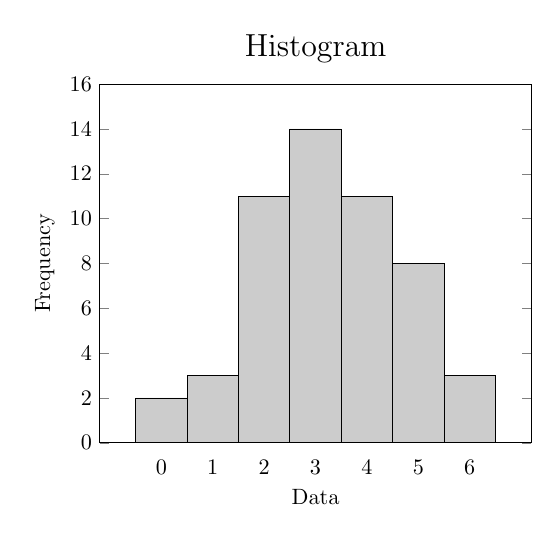
\begin{tikzpicture}[scale=0.8]
      \begin{axis}[
          title=\Large{Histogram},
          ymin=0, ymax=16,
          ytick={0, 2, ..., 16},
          xlabel=Data, ylabel=Frequency,
          ybar interval,
          grid=none,
          xtick style={draw=none},
        ]
        \addplot+[draw=black, style={fill=gray!40},mark=no] plot coordinates { (0, 2) (1, 3) (2, 11) (3, 14) (4, 11) (5, 8) (6, 3) (7, 0) };
      \end{axis}
    \end{tikzpicture}
  \end{center}

  The frequency polygon is a continuous line graph, the x-axis is the midpoint of
  each class, and the y-axis is the frequency of each class. To draw a frequency
  polygon, we plot each point, including the point before the first class and the
  point after the last class that uses $0$ as their frequency, and then connect
  the points with a continuous line.

  \begin{center}
    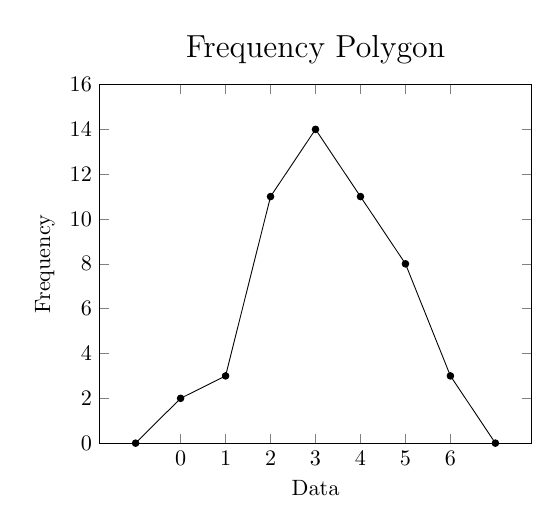
\begin{tikzpicture}[scale=0.8]
      \begin{axis}[
          title=\Large{Frequency Polygon},
          ymin=0, ymax=16,
          ytick={0, 2, ..., 16},
          xtick={0,1,...,6},
          xlabel=Data, ylabel=Frequency,
        ]
        \addplot[sharp plot, mark=*, mark size=1.5pt, mark options={solid, fill=black, draw=black}, draw=black]
        coordinates
          {(-1, 0) (0, 2) (1, 3) (2, 11) (3, 14) (4, 11) (5, 8) (6, 3) (7, 0)};
      \end{axis}
    \end{tikzpicture}
  \end{center}

  \begin{center}
    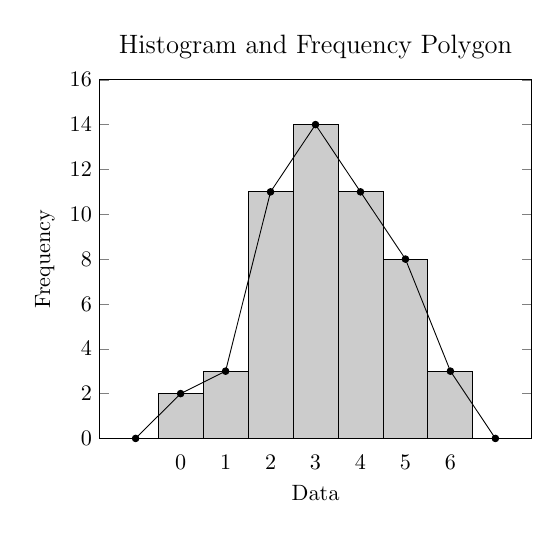
\begin{tikzpicture}[scale=0.8]
      \begin{axis}[
          title=\large{Histogram and Frequency Polygon},
          ymin=0, ymax=16,
          ytick={0, 2, ..., 16},
          xtick={0,1,...,6},
          ybar interval,
          grid=none,
          xtick style={draw=none},
          xlabel=Data, ylabel=Frequency,
        ]
        \addplot[draw=black, style={fill=gray!40},mark=no] plot coordinates { (0, 2) (1, 3) (2, 11) (3, 14) (4, 11) (5, 8) (6, 3) (7, 0) };
        \addplot[forget plot, sharp plot, mark=*, mark size=1.5pt, mark options={solid, fill=black, draw=black}, draw=black]
        coordinates
          {(-0.5, 0) (0.5, 2) (1.5, 3) (2.5, 11) (3.5, 14) (4.5, 11) (5.5, 8) (6.5, 3) (7.5, 0)};
      \end{axis}
    \end{tikzpicture}
  \end{center}

  \subsection{Practice 1}

  There are 105 students in a senior 3 art and commerce class. In a mock exam of
  UEC, their scores for Mathematics subject are as follows:
  \begin{flalign*}
    35 & \qquad 88 \qquad 67 \qquad 32 \qquad 38 \qquad 34 \qquad 45 \\
    78 & \qquad 54 \qquad 58 \qquad 69 \qquad 21 \qquad 90 \qquad 78 \\
    74 & \qquad 43 \qquad 42 \qquad 35 \qquad 57 \qquad 34 \qquad 77 \\
    89 & \qquad 66 \qquad 74 \qquad 71 \qquad 44 \qquad 56 \qquad 48 \\
    33 & \qquad 24 \qquad 73 \qquad 63 \qquad 51 \qquad 59 \qquad 49 \\
    34 & \qquad 55 \qquad 52 \qquad 75 \qquad 72 \qquad 62 \qquad 62 \\
    44 & \qquad 48 \qquad 73 \qquad 49 \qquad 57 \qquad 67 \qquad 80 \\
    70 & \qquad 66 \qquad 54 \qquad 32 \qquad 29 \qquad 35 \qquad 37 \\
    47 & \qquad 41 \qquad 51 \qquad 36 \qquad 46 \qquad 55 \qquad 53 \\
    60 & \qquad 53 \qquad 62 \qquad 39 \qquad 35 \qquad 48 \qquad 42 \\
    71 & \qquad 63 \qquad 70 \qquad 33 \qquad 45 \qquad 42 \qquad 44 \\
    61 & \qquad 59 \qquad 67 \qquad 30 \qquad 42 \qquad 43 \qquad 89 \\
    96 & \qquad 82 \qquad 47 \qquad 63 \qquad 54 \qquad 34 \qquad 45 \\
    45 & \qquad 87 \qquad 28 \qquad 34 \qquad 29 \qquad 77 \qquad 64 \\
    64 & \qquad 50 \qquad 48 \qquad 75 \qquad 33 \qquad 56 \qquad 84
  \end{flalign*}

  \begin{enumerate}[label=(\alph*)]
    \item Find the range of the data. \sol{}
          \begin{flalign*}
            \text{Max value}         & = 96      \\
            \text{Min value}         & = 21      \\
            \therefore\ \text{Range} & = 96 - 21 \\
                                     & = 75
          \end{flalign*}

    \item Group the data into 10 classes, draw a frequency distribution table, and find
          the upper and lower boundary and midpoint of each class. \sol{}
          \begin{flalign*}
            \text{Range}             & = 75            \\
            \text{Number of classes} & = 10            \\
            \text{Class width}       & = \frac{75}{10} \\
                                     & = 7.5           \\
                                     & \approx 8
          \end{flalign*}
          \begin{center}
            \begin{tabular}{|c|c|c|c|c|}
              \hline
              \text{Score} & \text{Lower} & \text{Upper} & \text{Mid} & \text{Freq.} \\
              \hline
              21 - 28      & 20.5         & 28.5         & 24.5       & 3            \\
              29 - 36      & 28.5         & 36.5         & 32.5       & 18           \\
              37 - 44      & 36.5         & 44.5         & 40.5       & 13           \\
              45 - 52      & 44.5         & 52.5         & 48.5       & 17           \\
              53 - 60      & 52.5         & 60.5         & 56.5       & 15           \\
              61 - 68      & 60.5         & 68.5         & 64.5       & 14           \\
              69 - 76      & 68.5         & 76.5         & 72.5       & 12           \\
              77 - 84      & 76.5         & 84.5         & 80.5       & 7            \\
              85 - 92      & 84.5         & 92.5         & 88.5       & 5            \\
              93 - 100     & 92.5         & 100.5        & 96.5       & 1            \\
              \hline
            \end{tabular}
          \end{center}
    \item Construct a histogram and frequency polygon. \sol{}
          \begin{center}
            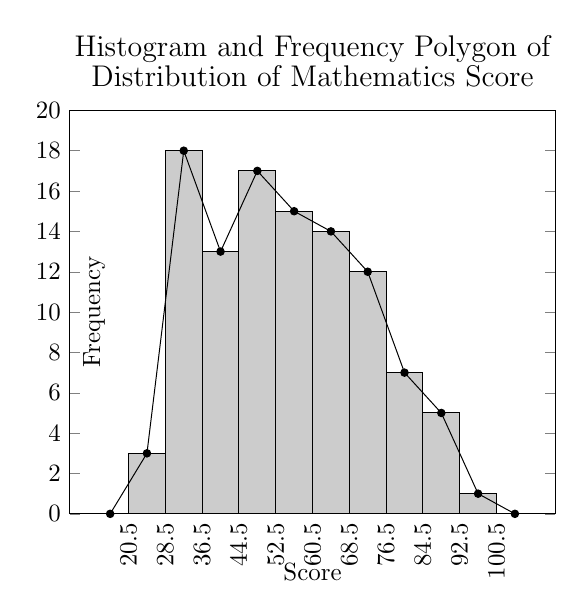
\begin{tikzpicture}[scale=0.9]
              \begin{axis}[
                  title style = {align = center},
                  title={\large{Histogram and Frequency Polygon of} \\ \large{Distribution of Mathematics Score}},
                  ymin=0, ymax=20,
                  ytick={0, 2, ..., 20},
                  xtick={20.5, 28.5, ..., 100.5},
                  grid=none,
                  xtick style={draw=none, fill=none, font=\footnotesize},
                  x tick label style = {rotate=90,anchor=east},
                  xlabel=Score, ylabel=Frequency,
                  xlabel style={at={(axis description cs:0.5, -0.1)}, anchor=north},
                  ylabel style={at={(axis description cs:0.05, 0.5)}, anchor=center},
                ]
                \addplot[ybar interval, draw=black, style={fill=gray!40},mark=no] plot coordinates { (20.5, 3) (28.5, 18) (36.5, 13) (44.5, 17) (52.5, 15) (60.5, 14) (68.5, 12) (76.5, 7) (84.5, 5) (92.5, 1) (100.5, 0) };
                \addplot[forget plot, sharp plot, mark=*, mark size=1.5pt, mark options={solid, fill=black, draw=black}, draw=black]
                coordinates
                  { (16.5, 0) (24.5, 3) (32.5, 18) (40.5, 13) (48.5, 17) (56.5, 15) (64.5, 14) (72.5, 12) (80.5, 7) (88.5, 5) (96.5, 1) (104.5, 0) };
              \end{axis}
            \end{tikzpicture}
          \end{center}
  \end{enumerate}

  \subsection*{Cumulative Frequency Distribution}

  Summing up the frequency of each class, we obtain the cumulative frequency
  distribution. Use the upper boundary of each class as the x-axis, and the
  cumulative frequency as the y-axis, we can draw the cumulative frequency
  distribution by plotting each point including the point before the first class
  that uses 0 as its frequency and connect them together. If we split the x-axis
  and the higest point of the curve into 100 equal parts, we get the percentage
  of the cumulative frequency distribution.

  \subsection{Practice 2}

  There are 155 students in a senior 3 art and commerce class, and the frequency
  distribution table of their average marks is shown below:

  \begin{center}
    \begin{tabular}{|c|c|}
      \hline
      \text{Average Mark} & \text{Frequency} \\
      \hline
      50 - 55             & 3                \\
      55 - 60             & 8                \\
      60 - 65             & 25               \\
      65 - 70             & 38               \\
      70 - 75             & 46               \\
      75 - 80             & 19               \\
      80 - 85             & 12               \\
      85 - 90             & 4                \\
      \hline
    \end{tabular}
  \end{center}

  \begin{enumerate}[label=(\alph*)]
    \item Make a cumulative frequency distribution table and draw a cumulative frequency
          polygon.

          \sol{}
          \begin{center}
            \begin{tabular}{|c|c|c|c|}
              \hline
              \text{Avg} & \text{Freq.} & \text{Lower Than} & \text{Cumm. Freq.} \\
              \hline
              50 - 55    & 3            & 55                & 3                  \\
              55 - 60    & 8            & 60                & 11                 \\
              60 - 65    & 25           & 65                & 36                 \\
              65 - 70    & 38           & 70                & 74                 \\
              70 - 75    & 46           & 75                & 120                \\
              75 - 80    & 19           & 80                & 139                \\
              80 - 85    & 12           & 85                & 151                \\
              85 - 90    & 4            & 90                & 155                \\
              \hline
            \end{tabular}
          \end{center}

          \begin{center}
            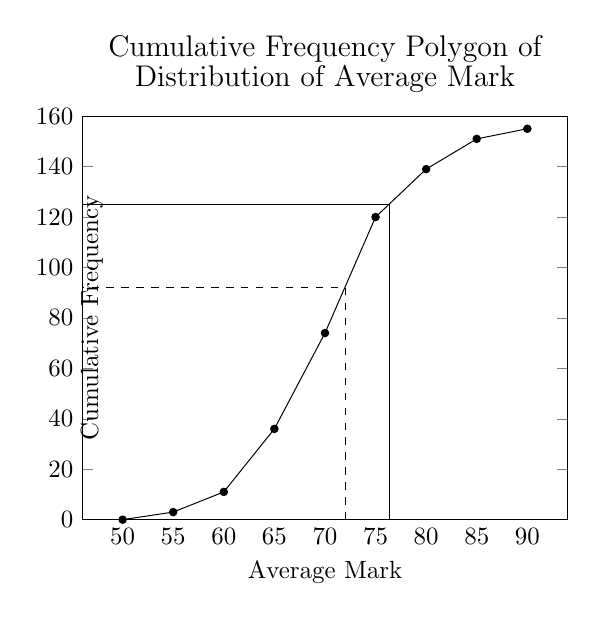
\begin{tikzpicture}[scale=0.9]
              \begin{axis}[
                  title style = {align = center},
                  title={\large{Cumulative Frequency Polygon of} \\ \large{Distribution of Average Mark}},
                  ymin=0, ymax=160,
                  ytick={0, 20, ..., 160},
                  xtick={50, 55, 60, ..., 90},
                  xtick style={draw=none, fill=none, font=\footnotesize},
                  xlabel=Average Mark, ylabel=Cumulative Frequency,
                  ylabel style={at={(axis description cs:0.02, 0.5)}, anchor=center},
                ]
                \addplot[forget plot, sharp plot, mark=*, mark size=1.5pt, mark options={solid, fill=black, draw=black}, draw=black]
                coordinates
                  { (50, 0) (55, 3) (60, 11) (65, 36) (70, 74) (75, 120) (80, 139) (85, 151) (90, 155) };
                \draw[dashed] (axis cs:72, 0) -- (axis cs:72, 92) -- (axis cs:0, 92);
                \draw (axis cs:0, 125) -- (axis cs:76.4, 125) -- (axis cs:76.4, 0);
              \end{axis}
            \end{tikzpicture}
          \end{center}

    \item If the average mark of a student is 72, find his rank in the class. \sol{}

          In the graph above, we can see that there are approximately 92 students who
          have an average mark lower than 72. Therefore, the rank of the student is $155
            - 92 = 63$.

    \item If the top $20\%$ of the class are to be awarded a certificate, find the
          minimum average mark required for the certificate. \sol{}
          \begin{flalign*}
            \text{Top $20\%$} & = 20\% \cdot 155 \\
                              & = 31
          \end{flalign*}
          Therefore, students with an average mark corresponding to cumulative frequency higher than 124 will be awarded a certificate.

          In the graph above, The minimum average mark required for the certificate is
          76.
  \end{enumerate}

  \subsection{Exercise 18.2}

  \begin{enumerate}
    \item A company performed an ability test on 100 job seekers and the results are
          shown in the following table:
          \begin{center}
            \begin{tabular}{|c|c|c|c|c|c|c|}
              \hline
              \text{Score}     & 8 & 7  & 6  & 5  & 4  & 3 \\
              \hline
              \text{Frequency} & 5 & 12 & 24 & 33 & 19 & 7 \\
              \hline
            \end{tabular}
          \end{center}
          Construct a hustogram and a frequency polygon for the data above.
          \sol{}
          \begin{center}
            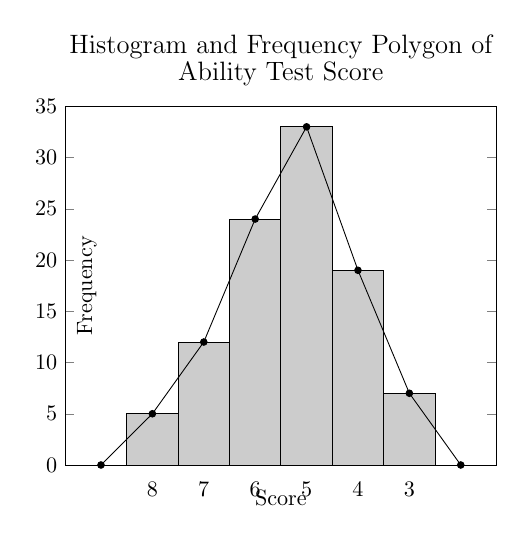
\begin{tikzpicture}[scale=0.8]
              \begin{axis}[
                  title style = {align = center},
                  title={\large{Histogram and Frequency Polygon of} \\ \large{Ability Test Score}},
                  ymin=0, ymax=35,
                  ytick={0, 5, ..., 35},
                  x dir=reverse,
                  ybar interval,
                  grid=none,
                  xtick style={draw=none},
                  xlabel=Score, ylabel=Frequency,
                  xlabel style={at={(axis description cs:0.5, -0.05)}, anchor=north},
                  ylabel style={at={(axis description cs:0.05, 0.5)}, anchor=center},
                ]
                \addplot[draw=black, style={fill=gray!40},mark=no] plot coordinates { (8, 5) (7, 12) (6, 24) (5, 33) (4, 19) (3, 7) (2, 0) };
                \addplot[forget plot, sharp plot, mark=*, mark size=1.5pt, mark options={solid, fill=black, draw=black}, draw=black]
                coordinates
                  {(8.5, 0) (7.5, 5) (6.5, 12) (5.5, 24) (4.5, 33) (3.5, 19) (2.5, 7) (1.5, 0)};
              \end{axis}
            \end{tikzpicture}
          \end{center}

    \item Take 120 ears of rice from a rice field, the length of each ear is measured (in
          $cm$) and the results are as following:
          \begin{flalign*}
            6.5 & \qquad 6.4 \qquad 6.7 \qquad 5.8 \qquad 5.9 \qquad 5.9 \\
            5.2 & \qquad 4.0 \qquad 5.4 \qquad 4.6 \qquad 5.8 \qquad 5.5 \\
            6.0 & \qquad 6.5 \qquad 5.1 \qquad 6.2 \qquad 5.4 \qquad 5.0 \\
            5.0 & \qquad 6.8 \qquad 6.0 \qquad 5.0 \qquad 5.7 \qquad 6.0 \\
            5.5 & \qquad 6.8 \qquad 6.0 \qquad 6.3 \qquad 5.5 \qquad 5.0 \\
            6.4 & \qquad 5.8 \qquad 5.9 \qquad 5.7 \qquad 6.8 \qquad 6.6 \\
            6.0 & \qquad 6.4 \qquad 5.7 \qquad 7.4 \qquad 6.0 \qquad 5.4 \\
            6.5 & \qquad 6.0 \qquad 6.8 \qquad 5.3 \qquad 6.4 \qquad 5.7 \\
            6.7 & \qquad 6.2 \qquad 5.6 \qquad 6.0 \qquad 6.7 \qquad 6.7 \\
            6.0 & \qquad 5.5 \qquad 6.2 \qquad 6.1 \qquad 5.3 \qquad 6.2 \\
            5.8 & \qquad 5.3 \qquad 7.0 \qquad 6.0 \qquad 6.0 \qquad 5.9 \\
            5.4 & \qquad 6.0 \qquad 5.2 \qquad 6.0 \qquad 6.3 \qquad 5.7 \\
            6.8 & \qquad 6.1 \qquad 4.5 \qquad 5.4 \qquad 6.3 \qquad 6.9 \\
            4.9 & \qquad 5.1 \qquad 5.6 \qquad 5.9 \qquad 6.1 \qquad 6.5 \\
            6.6 & \qquad 5.7 \qquad 5.8 \qquad 5.8 \qquad 6.2 \qquad 6.3 \\
            6.5 & \qquad 5.3 \qquad 5.9 \qquad 5.5 \qquad 5.8 \qquad 6.3 \\
            5.2 & \qquad 6.0 \qquad 7.0 \qquad 6.4 \qquad 5.8 \qquad 6.3 \\
            6.0 & \qquad 6.3 \qquad 5.6 \qquad 6.8 \qquad 6.6 \qquad 4.7 \\
            5.7 & \qquad 5.7 \qquad 5.6 \qquad 6.3 \qquad 6.0 \qquad 5.8 \\
            6.3 & \qquad 7.5 \qquad 6.2 \qquad 6.4 \qquad 7.0 \qquad 6.5
          \end{flalign*}

          \begin{enumerate}
            \item Find the range of the dataset. \sol{}
                  \begin{flalign*}
                    \text{Min value}         & = 4.0       \\
                    \text{Max value}         & = 7.5       \\
                    \therefore\ \text{Range} & = 7.5 - 4.0 \\
                                             & = 3.5
                  \end{flalign*}
            \item Group the data into 12 classes, make a frequency distribution table, find the
                  upper and lower boundaries and midpoint of each class, and calculate the
                  cumulative frequency. \sol{}
                  \begin{flalign*}
                    \text{Range}                   & = 3.5            \\
                    \text{Number of classes}       & = 12             \\
                    \therefore\ \text{Class width} & = \frac{3.5}{12} \\
                                                   & = \frac{3.5}{12} \\
                                                   & \approx 0.3
                  \end{flalign*}
                  \begin{center}
                    \begin{tabular}{|c|c|c|c|c|}
                      \hline
                      Weight    & Lower & Upper & Mid  & Freq. \\
                      \hline
                      4.0 - 4.2 & 3.95  & 4.25  & 4.10 & 1     \\
                      4.3 - 4.5 & 4.25  & 4.55  & 4.40 & 1     \\
                      4.6 - 4.8 & 4.55  & 4.85  & 4.70 & 2     \\
                      4.9 - 5.1 & 4.85  & 5.15  & 5.00 & 7     \\
                      5.2 - 5.4 & 5.15  & 5.45  & 5.30 & 12    \\
                      5.5 - 5.7 & 5.45  & 5.75  & 5.60 & 17    \\
                      5.8 - 6.0 & 5.75  & 6.05  & 5.90 & 31    \\
                      6.1 - 6.3 & 6.05  & 6.35  & 6.20 & 18    \\
                      6.4 - 6.6 & 6.35  & 6.65  & 6.50 & 15    \\
                      6.7 - 6.9 & 6.65  & 6.95  & 6.80 & 11    \\
                      7.0 - 7.2 & 6.95  & 7.25  & 7.10 & 3     \\
                      7.3 - 7.5 & 7.25  & 7.55  & 7.40 & 2     \\
                      \hline
                    \end{tabular}
                  \end{center}
                  \begin{center}
                    \begin{tabular}{|c|c|c|c|}
                      \hline
                      Weight    & Freq. & Lower Than & Cum. Freq. \\
                      \hline
                      4.0 - 4.3 & 1     & 4.3        & 1          \\
                      4.3 - 4.6 & 1     & 4.6        & 2          \\
                      4.6 - 4.9 & 2     & 4.9        & 4          \\
                      4.9 - 5.2 & 7     & 5.2        & 11         \\
                      5.2 - 5.5 & 12    & 5.5        & 23         \\
                      5.5 - 5.8 & 17    & 5.8        & 40         \\
                      5.8 - 6.1 & 31    & 6.1        & 71         \\
                      6.1 - 6.4 & 18    & 6.4        & 89         \\
                      6.4 - 6.7 & 15    & 6.7        & 104        \\
                      6.7 - 7.0 & 11    & 7.0        & 115        \\
                      7.0 - 7.3 & 3     & 7.3        & 118        \\
                      7.3 - 7.6 & 2     & 7.6        & 120        \\
                      \hline
                    \end{tabular}
                  \end{center}

            \item Construct a frequency polygon. \sol{}
                  \begin{center}
                    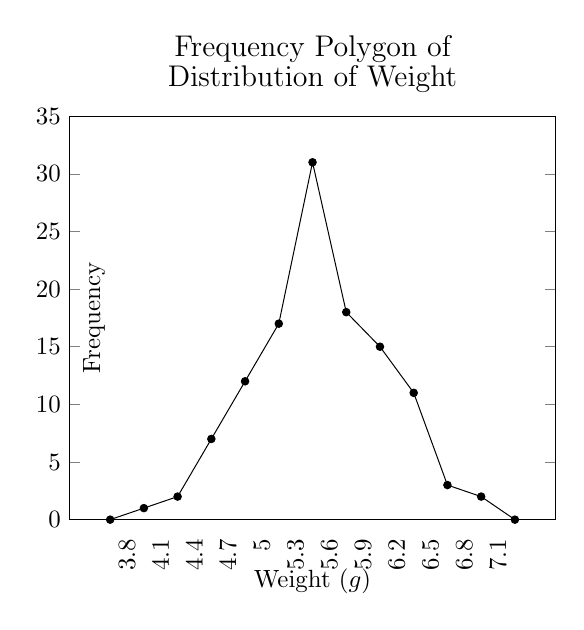
\begin{tikzpicture}[scale=0.9]
                      \begin{axis}[
                          title style = {align = center},
                          title={\large{Frequency Polygon of} \\ \large{Distribution of Weight}},
                          ymin=0, ymax=35,
                          ytick={0, 5, ..., 35},
                          ybar interval,
                          grid=none,
                          xtick style={draw=none, fill=none, font=\footnotesize},
                          x tick label style = {rotate=90,anchor=east},
                          xlabel=Weight ($g$), ylabel=Frequency,
                          xlabel style={at={(axis description cs:0.5, -0.1)}, anchor=north},
                          ylabel style={at={(axis description cs:0.05, 0.5)}, anchor=center},
                        ]
                        \addplot[forget plot, sharp plot, mark=*, mark size=1.5pt, mark options={solid, fill=black, draw=black}, draw=black]
                        coordinates
                          { (3.8, 0) (4.1, 1) (4.4, 2) (4.7, 7) (5.0, 12) (5.3, 17) (5.6, 31) (5.9, 18) (6.2, 15) (6.5, 11) (6.8, 3) (7.1, 2) (7.4, 0) };
                      \end{axis}
                    \end{tikzpicture}
                  \end{center}

            \item Construct a cumulative frequency polygon. \sol{}
                  \begin{center}
                    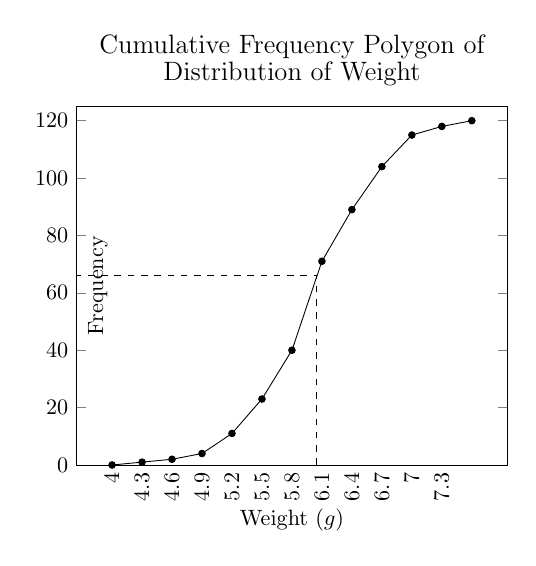
\begin{tikzpicture}[scale=0.8]
                      \begin{axis}[
                        title style = {align = center},
                        title={\large{Cumulative Frequency Polygon of} \\ \large{Distribution of Weight}},
                        ymin=0, ymax=125,
                        ytick={0, 20, ..., 120},
                        xtick={4.0, 4.3, 4.6, ..., 7.4},
                        xtick style={draw=none, fill=none, font=\footnotesize}, x tick label style =
                          {rotate=90,anchor=east}, xlabel=Weight ($g$), ylabel=Frequency, xlabel
                        style={at={(axis description cs:0.5, -0.1)}, anchor=north}, ylabel
                        style={at={(axis description cs:0.05, 0.5)}, anchor=center}, ] \addplot[forget
                          plot, sharp plot, mark=*, mark size=1.5pt, mark options={solid, fill=black,
                              draw=black}, draw=black] coordinates { (4.0, 0) (4.3, 1) (4.6, 2) (4.9, 4)
                            (5.2, 11) (5.5, 23) (5.8, 40) (6.1, 71) (6.4, 89) (6.7, 104) (7.0, 115) (7.3,
                            118) (7.6, 120) };
                        \draw [dashed] (axis cs: 6.05, 0) -- (axis cs: 6.05, 66) -- (axis cs: 0, 66);
                      \end{axis}
                    \end{tikzpicture}
                  \end{center}

            \item Find the percentage of the ears of rice whose length is greater than $6cm$.
                  \sol{}

                  In the diagram above, there are approximately $120 - 66 = 54$ ears of rice
                  whose length is greater than $6cm$, which is about $\frac{54}{120} \cdot 100\%
                    = 45\%$ of the total number of ears of rice.

          \end{enumerate}

    \item The table below shows the weight distribution of 90 babies (in $kg$):
          \begin{center}
            \begin{tabular}{|c|c|}
              \hline
              Weight    & Frequency \\
              \hline
              1.5 - 2.0 & 2         \\
              2.0 - 2.5 & 4         \\
              2.5 - 3.0 & 13        \\
              3.0 - 3.5 & 32        \\
              3.5 - 4.0 & 28        \\
              4.0 - 4.5 & 10        \\
              4.5 - 5.0 & 1         \\
              \hline
            \end{tabular}
          \end{center}
          \begin{enumerate}
            \item Make a cumulative frequency table. \sol{}
                  \begin{center}
                    \begin{tabular}{|c|c|c|c|}
                      \hline
                      Weight    & Freq. & Less than & Cum. Freq. \\
                      \hline
                      1.5 - 2.0 & 2     & 2.0       & 2          \\
                      2.0 - 2.5 & 4     & 2.5       & 6          \\
                      2.5 - 3.0 & 13    & 3.0       & 19         \\
                      3.0 - 3.5 & 32    & 3.5       & 51         \\
                      3.5 - 4.0 & 28    & 4.0       & 79         \\
                      4.0 - 4.5 & 10    & 4.5       & 89         \\
                      4.5 - 5.0 & 1     & 5.0       & 90         \\
                      \hline
                    \end{tabular}
                  \end{center}

            \item Construct a cumulative frequency polygon. \sol{}
                  \begin{center}
                    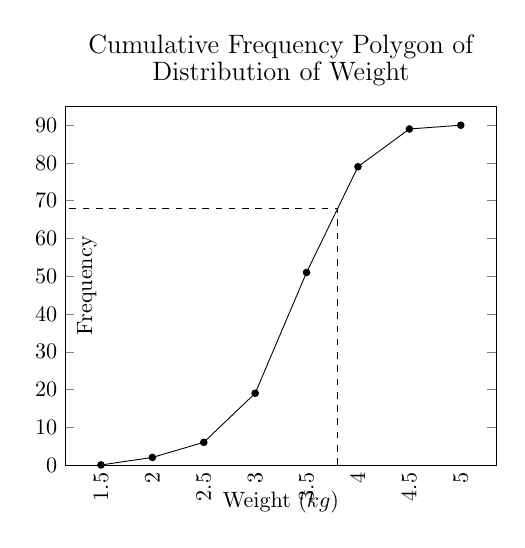
\begin{tikzpicture}[scale=0.8]
                      \begin{axis}[
                        title style = {align = center},
                        title={\large{Cumulative Frequency Polygon of} \\ \large{Distribution of Weight}},
                        ymin=0, ymax=95,
                        ytick={0, 10, ..., 90},
                        xtick={1.5, 2.0, 2.5, ..., 5.0},
                        xtick style={draw=none, fill=none, font=\footnotesize}, x tick label style =
                          {rotate=90,anchor=east}, xlabel=Weight ($kg$), ylabel=Frequency, xlabel
                        style={at={(axis description cs:0.5, -0.05)}, anchor=north}, ylabel
                        style={at={(axis description cs:0.05, 0.5)}, anchor=center}, ] \addplot[forget
                          plot, sharp plot, mark=*, mark size=1.5pt, mark options={solid, fill=black,
                              draw=black}, draw=black] coordinates { (1.5, 0) (2.0, 2) (2.5, 6) (3.0, 19)
                            (3.5, 51) (4.0, 79) (4.5, 89) (5.0, 90) };
                        \draw [dashed] (axis cs: 3.8, 0) -- (axis cs: 3.8, 68) -- (axis cs: 0, 68);
                      \end{axis}
                    \end{tikzpicture}
                  \end{center}

            \item Find the percentage of babies whose weight is greater than $3.8kg$. \sol{}

                  In the diagram above, there are approximately $90 - 68 = 22$ babies whose
                  weight is greater than $3.8kg$, which is about $\frac{22}{90} \cdot 100\% =
                    24.44\%$ of the total number of babies.
          \end{enumerate}

    \item The table below shows the average score distribution of 50 students in a class:
          \begin{center}
            \begin{tabular}{|c|c|}
              \hline
              Average Score & Frequency \\
              \hline
              50.0 - 59.9   & 4         \\
              60.0 - 69.9   & 9         \\
              70.0 - 79.9   & 23        \\
              80.0 - 89.9   & 12        \\
              90.0 - 99.9   & 2         \\
              \hline
            \end{tabular}
          \end{center}
          \begin{enumerate}
            \item Make a cumulative frequency table and draw a cumulative frequency polygon.
                  \sol{}
                  \begin{center}
                    \begin{tabular}{|c|c|c|c|}
                      \hline
                      Average Score & Freq. & Less than & Cum. Freq. \\
                      \hline
                      50.0 - 59.9   & 4     & 60        & 4          \\
                      60.0 - 69.9   & 9     & 70        & 13         \\
                      70.0 - 79.9   & 23    & 80        & 36         \\
                      80.0 - 89.9   & 12    & 90        & 48         \\
                      90.0 - 99.9   & 2     & 100       & 50         \\
                      \hline
                    \end{tabular}
                  \end{center}
                  \begin{center}
                    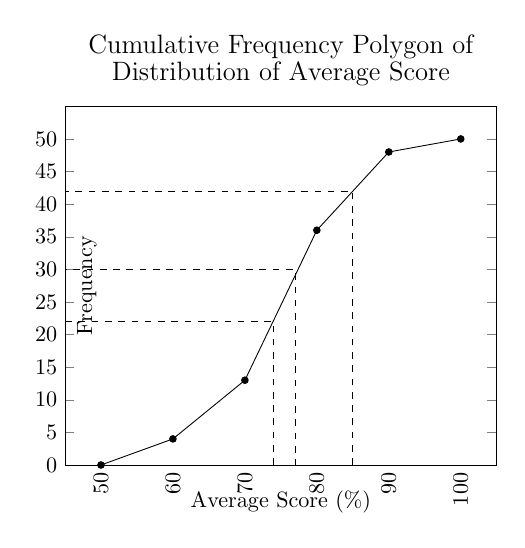
\begin{tikzpicture}[scale=0.8]
                      \begin{axis}[
                        title style = {align = center},
                        title={\large{Cumulative Frequency Polygon of} \\ \large{Distribution of Average Score}},
                        ymin=0, ymax=55,
                        ytick={0, 5, ..., 50},
                        xtick={50, 60, 70, 80, 90, 100},
                        xtick style={draw=none, fill=none, font=\footnotesize}, x tick label style =
                          {rotate=90,anchor=east}, xlabel=Average Score ($\%$), ylabel=Frequency, xlabel
                        style={at={(axis description cs:0.5, -0.05)}, anchor=north}, ylabel
                        style={at={(axis description cs:0.05, 0.5)}, anchor=center}, ] \addplot[forget
                          plot, sharp plot, mark=*, mark size=1.5pt, mark options={solid, fill=black,
                              draw=black}, draw=black] coordinates { (50, 0) (60, 4) (70, 13) (80, 36)
                            (90, 48) (100, 50) };
                        \draw [dashed] (axis cs: 74, 0) -- (axis cs: 74, 22) -- (axis cs: 0, 22);
                        \draw [dashed] (axis cs: 0, 30) -- (axis cs: 77, 30) -- (axis cs: 77, 0);
                        \draw [dashed] (axis cs: 85, 0) -- (axis cs: 85, 42) -- (axis cs: 0, 42);
                      \end{axis}
                    \end{tikzpicture}
                  \end{center}

            \item A student get an average score of $74$, find his rank in the class. \sol{}

                  In the diagram above, there are approximately $22$ students whose average score
                  is less than $74$, which means that the student is ranked $50 - 22 = 28$.

            \item Find the average score of the student who is ranked $20$. \sol{}

                  In the diagram above, the student who is ranked $20$ has an average score of
                  about $77$.

            \item Find the percentage of students whose average score is greater than $85$.
                  \sol{}

                  In the diagram above, there are approximately $50 - 42 = 8$ students whose
                  average score is greater than $85$, which is about $\frac{8}{50} \cdot 100\% =
                    16\%$ of the total number of students.
          \end{enumerate}

    \item The table below shows the score distribution of 1200 students in UEC accounting
          exam:
          \begin{center}
            \begin{tabular}{|c|c|}
              \hline
              Score   & Number of Students \\
              \hline
              10 - 19 & 20                 \\
              20 - 29 & 60                 \\
              30 - 39 & 95                 \\
              40 - 49 & 130                \\
              50 - 59 & 340                \\
              60 - 69 & 310                \\
              70 - 79 & 135                \\
              80 - 89 & 80                 \\
              90 - 99 & 30                 \\
              \hline
            \end{tabular}
          \end{center}
          Examinees are categorised into 4 groups based on their score: \textit{Excellent}, \textit{Good}, \textit{Pass}, and \textit{Fail}.
          \begin{enumerate}
            \item Make a cumulative frequency table and draw a cumulative frequency polygon.
                  \sol{}
                  \begin{center}
                    \begin{tabular}{|c|c|c|c|}
                      \hline
                      Score   & Freq. & Less than & Cum. Freq. \\
                      \hline
                      10 - 19 & 20    & 20        & 20         \\
                      20 - 29 & 60    & 80        & 80         \\
                      30 - 39 & 95    & 175       & 175        \\
                      40 - 49 & 130   & 305       & 305        \\
                      50 - 59 & 340   & 645       & 645        \\
                      60 - 69 & 310   & 955       & 955        \\
                      70 - 79 & 135   & 1090      & 1090       \\
                      80 - 89 & 80    & 1170      & 1170       \\
                      90 - 99 & 30    & 1200      & 1200       \\
                      \hline
                    \end{tabular}
                  \end{center}
                  \begin{center}
                    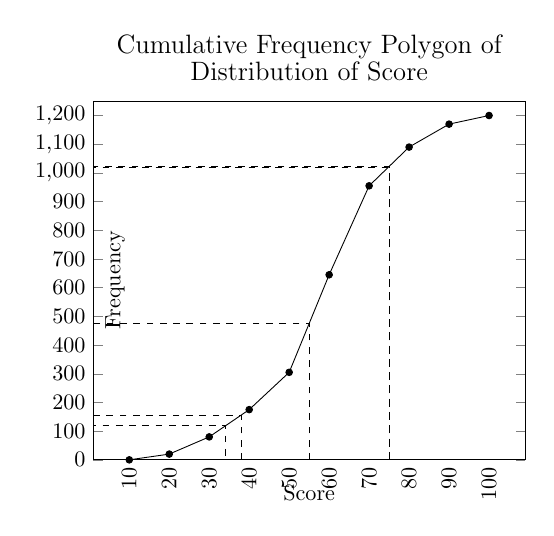
\begin{tikzpicture}[scale=0.8]
                      \begin{axis}[
                          title style = {align = center},
                          title={\large{Cumulative Frequency Polygon of} \\ \large{Distribution of Score}},
                          ymin=0, ymax=1250,
                          ytick={0, 100, ..., 1200},
                          xtick={10, 20, 30, 40, 50, 60, 70, 80, 90, 100},
                          xtick style={draw=none, fill=none, font=\footnotesize}, x tick label style =
                            {rotate=90,anchor=east}, xlabel=Score, ylabel=Frequency, xlabel style={at={(axis
                                  description cs:0.5, -0.05)}, anchor=north}, ylabel style={at={(axis
                                  description cs:0.05, 0.5)}, anchor=center}, ] \addplot[forget plot, sharp
                          plot, mark=*, mark size=1.5pt, mark options={solid, fill=black, draw=black},
                          draw=black] coordinates { (10, 0) (20, 20) (30, 80) (40, 175) (50, 305) (60,
                            645) (70, 955) (80, 1090) (90, 1170) (100, 1200) };
                        \draw [dashed] (axis cs: 38, 0) -- (axis cs: 38, 155) -- (axis cs: 0, 155);
                        \draw [dashed] (axis cs: 75, 0) -- (axis cs: 75, 1024) -- (axis cs: 0, 1024);
                        \draw [dashed] (axis cs: 55, 0) -- (axis cs: 55, 475) -- (axis cs: 0, 475);
                        \draw [dashed] (axis cs: 0, 120) -- (axis cs: 34, 120) -- (axis cs: 34, 0);
                        \draw [dashed] (axis cs: 0, 1020) -- (axis cs: 75, 1020) -- (axis cs: 75, 0);
                      \end{axis}
                    \end{tikzpicture}
                  \end{center}

            \item If the passing score is $38$, find the percentage of students who pass the
                  exam. \sol{}

                  In the diagram above, there are approximately $1200 - 155 = 1045$ students
                  whose score is greater or equal to $38$, which is about $\frac{1045}{1200}
                    \cdot 100\% = 86.67\%$ of the total number of students.

            \item Assume that the minimum score to be categorised as \textit{Excellent} and
                  \textit{Good} is $75$ and $55$ respectively, find the percentage of students
                  who are categorised as \textit{Excellent} and \textit{Good} respectively.
                  \sol{}

                  In the diagram above, there are approximately $1200 - 1024 = 176$ students
                  whose score is greater or equal to $75$, which is about $\frac{176}{1200} \cdot
                    100\% = 14.67\%$ of the total number of students who are categorised as
                  \textit{Excellent}.

                  Also, there are approximately $1024 - 475 = 549$ students whose score is
                  greater or equal to $55$, which is about $\frac{549}{1200} \cdot 100\% =
                    45.75\%$ of the total number of students who are categorised as \textit{Good}.

            \item Find the passing mark if the percentage of students who pass the exam is
                  $90\%$. \sol{}

                  If the percentage of students who pass the exam is $90\%$, then the number of
                  students who pass the exam is $90\%$ of $1200$ students, which is $1080$
                  students. That means, there are $1200 - 1080 = 120$ students who fail the exam.

                  In the diagram above, the passing mark is about $34$ given that there are $120$
                  students who fail the exam.

            \item Find the minimum mark of a student who is categorised as \textit{Excellent} if
                  the percentage of students who are categorised as \textit{Excellent} is $15\%$.
                  \sol{}

                  If the percentage of students who are categorised as \textit{Excellent} is
                  $15\%$, then the number of students who are categorised as \textit{Excellent}
                  is $15\%$ of $1200$ students, which is $180$ students. That means, there are
                  $1200 - 180 = 1020$ students who are not categorised as \textit{Excellent}.

                  In the diagram above, the minimum mark of a student who is categorised as
                  \textit{Excellent} is about $75$ given that there are $1020$ students who are
                  not categorised as \textit{Excellent}.
          \end{enumerate}

  \end{enumerate}

  \section{Central Tendency}

  Central tendency is a measure of the central position of a distribution, or a
  single value that attempts to describe a set of data. The most common measures
  of central tendency are the mean, median, and mode.

  \subsection*{Mean}

  Mean is also known as arithmetic mean. For $n$ values $x_1, x_2, \ldots, x_n$,
  the mean is defined as \makeatletter \setbool{@fleqn}{false} \makeatother
  \begin{flalign*}
    \bar{x} & = \frac{x_1 + x_2 + \cdots + x_n}{n} \\
            & = \frac{\sum x_i}{n}
  \end{flalign*}
  \makeatletter
  \setbool{@fleqn}{true}
  \makeatother

  For data whose possible values are $x_1, x_2, \ldots, x_n$, and their
  respective frequencies are $f_1, f_2, \ldots, f_n$, the mean is defined as
  \makeatletter \setbool{@fleqn}{false} \makeatother
  \begin{flalign*}
    \bar{x} & = \frac{x_1f_1 + x_2f_2 + \cdots + x_nf_n}{f_1 + f_2 + \cdots + f_n} \\
            & = \frac{\sum f_i x_i}{\sum f_i}
  \end{flalign*}
  \makeatletter
  \setbool{@fleqn}{true}
  \makeatother

  For grouped data, we take the mean of each class as the representative value
  $x_i$ of the class.

  \subsubsection*{Weighted Mean}

  In some scenario, weighted mean is better than the mean to describe the data.

  When calculating the arithmetic mean, each value is given equal weight.
  However, in some cases, each value in a dataset may not be equally important.
  For example, the importance of the mark of a student for each subject is
  weighted according to the number of classes of the subject in a week. Hence,
  when calculating the average mark of the student, each mark must be multiplied
  by a value that represents the importance of the subject, and that value is
  called the weight. The weighted mean is defined as \makeatletter
  \setbool{@fleqn}{false} \makeatother
  \begin{flalign*}
    \bar{x} & = \frac{w_1x_1 + w_2x_2 + \cdots + w_n x_n}{w_1 + w_2 + \cdots + w_n} \\
            & = \frac{\sum w_i x_i}{\sum w_i}
  \end{flalign*}
  \makeatletter
  \setbool{@fleqn}{true}
  \makeatother
  where $x_i$ are the values and $w_i$ are the weights of $x_i$.

  \subsection{Practice 3}

  \begin{enumerate}
    \item Find the mean of 34, 50, 24, 32, 53, 30, 62, 27. \sol{}
          \begin{flalign*}
            \bar{x} & = \frac{30 + 50 + 24 + 32 + 53 + 30 + 62 + 27}{8} \\
                    & = \frac{312}{8}                                   \\
                    & = 39
          \end{flalign*}

    \item There are three workshop $A$, $B$, and $C$ in a factory. Workshop $A$ has 10
          workers, their wages are $\$35$ per day, workshop $B$ has 30 workers, their
          wages are $\$45$ per day, and workshop $C$ has 15 workers, their wages are
          $\$55$ per day. Find the mean of the wages of the workers in the factory.
          \sol{}

          Let the wages of workers be $x_1$, and the amount of workers be $f_1$.
          \begin{center}
            \begin{tabular}{|c|c|c|}
              \hline
              $x_1$ & $f_1$           & $x_1f_1$              \\
              \hline
              35    & 10              & 350                   \\
              45    & 30              & 1350                  \\
              55    & 15              & 825                   \\
              \hline
                    & $\sum f_i = 55$ & $\sum f_i x_i = 2525$ \\
              \hline
            \end{tabular}
          \end{center}
          $\therefore $ Average wages of workers in the factory is $\frac{2525}{55} = \$45.91$.

    \item A school appoints students to participate in a Math competition. During the
          competition, candidates must answer 25 questions within an hour. The table
          below shows the distribution of frequency of the number of questions that those
          candidates answer correctly:
          \begin{center}
            \begin{tabular}{|c|c|}
              \hline
              Answered Correctly & Frequency \\
              \hline
              1 - 5              & 3         \\
              6 - 10             & 12        \\
              11 - 15            & 7         \\
              16 - 20            & 8         \\
              21 - 25            & 5         \\
              \hline
            \end{tabular}
          \end{center}
          Complete the following table, and find the mean of the number of questions that those candidates answer correctly.
          \begin{center}
            \begin{tabular}{|c|c|c|c|}
              \hline
              Ans. Correctly & Freq. $f_i$ & Midpoint $x_i$ & $f_ix_i$ \\
              \hline
              1 - 5          &             &                &          \\
              6 - 10         &             &                &          \\
              11 - 15        &             &                &          \\
              16 - 20        &             &                &          \\
              21 - 25        &             &                &          \\
              \hline
            \end{tabular}
          \end{center}
          \sol{}
          \begin{center}
            \begin{tabular}{|c|c|c|c|}
              \hline
              Ans. Correctly & Freq. $f_i$     & Midpoint $x_i$       & $f_ix_i$ \\
              \hline
              1 - 5          & 3               & 3                    & 9        \\
              6 - 10         & 12              & 8                    & 96       \\
              11 - 15        & 7               & 13                   & 91       \\
              16 - 20        & 8               & 18                   & 144      \\
              21 - 25        & 5               & 23                   & 115      \\
              \hline
                             & $\sum f_i = 35$ & $\sum f_i x_i = 455$ &          \\
              \hline
            \end{tabular}
          \end{center}
          $\therefore $ The mean of the number of questions that those candidates answer correctly is $\frac{455}{35} = 13$.
  \end{enumerate}

  \subsection{Exercise 18.3a}

  \begin{enumerate}
    \item Take a sample of 20 from a batch of machine parts, their weight (in $g$) are as
          follows:
          \begin{flalign*}
            210 & \qquad 208 \qquad 200 \qquad 205 \qquad 202 \qquad 218 & \\
            206 & \qquad 214 \qquad 215 \qquad 207 \qquad 195 \qquad 207   \\
            218 & \qquad 192 \qquad 202 \qquad 216 \qquad 185 \qquad 227   \\
            187 & \qquad 215
          \end{flalign*}
          Find the mean weight of these machine parts.
          \sol{}
          \begin{flalign*}
            \bar{x} & = \frac{210 + 208 + 200 + \cdots + 215}{20} \\
                    & = \frac{4129}{20}                           \\
                    & = 206.45
          \end{flalign*}

    \item Given that the mean of a dataset 4, -3, 2, $k$, 5, 8 is 10, find the value of
          $k$. \sol{}
          \begin{flalign*}
            \frac{4 + (-3) + 2 + k + 5 + 8}{6} & = 10 \\
            16 + k                             & = 60 \\
            k                                  & = 44
          \end{flalign*}

    \item Given that the mean of $x_1$, $x_2$, $x_3$, $x_4$, $x_5$ is 40, and the mean of
          $y_1$, $y_2$, $y_3$ is 15. Find the mean after combining these two datasets.
          \sol{}
          \begin{flalign*}
            \frac{x_1 + \cdots + x_5}{5} & = 40                                 \\
            x_1 + \cdots + x_5           & = 200                                \\
            \\
            \frac{y_1 + y_2 + y_3}{3}    & = 15                                 \\
            y_1 + y_2 + y_3              & = 45                                 \\
            \\
            \bar{xy}                     & = \frac{x_1 + x_2 + \cdots + y_3}{8} \\
                                         & = \frac{245}{8}                      \\
                                         & = 30.63
          \end{flalign*}

    \item A school have 2 senior 3 classes: $A$ and $B$. In a Chinese language test, the
          average mark of 49 students in $A$ class in 72, while the average mark for 45
          students in class $B$ is 68. Find the average mark of all students in these two
          class combined. \sol{}
          \begin{flalign*}
            \bar{x} & = \frac{72 \cdot 49 + 68 \cdot 45}{49 + 45} \\
                    & = \frac{3528 + 3060}{94}                    \\
                    & = \frac{6588}{94}                           \\
                    & = 70.09
          \end{flalign*}

    \item Given that the mean for 8 values are 5. The mean increased by 1.4 after adding
          two values: $x$ and $3x$. Find the value of $x$. \sol{}
          \begin{flalign*}
            \frac{8 \cdot 5 + x + 3x}{8 + 2} & = 5 + 1.4 \\
            \frac{40 + 4x}{10}               & = 6.4     \\
            40 + 4x                          & = 64      \\
            4x                               & = 24      \\
            x                                & = 6
          \end{flalign*}
    \item Throwing 6 coin at the same time and record the number of heads. After throwing
          100 times, we get the following frequency distribution table:
          \begin{center}
            \begin{tabular}{|c|c|}
              \hline
              Number of Heads & Frequency \\
              \hline
              0               & 2         \\
              1               & 10        \\
              2               & 24        \\
              3               & 35        \\
              4               & 22        \\
              5               & 6         \\
              6               & 1         \\
              \hline
            \end{tabular}
          \end{center}
          Find the mean of the number of heads for each throw.
          \sol{}

          Let the number of heads be $x_i$ and the frequency be $f_i$.
          \begin{center}
            \begin{tabular}{|c|c|c|}
              \hline
              $x_i$ & $f_i$            & $x_i f_i$           \\
              \hline
              0     & 2                & 0                   \\
              1     & 10               & 10                  \\
              2     & 24               & 48                  \\
              3     & 35               & 105                 \\
              4     & 22               & 88                  \\
              5     & 6                & 30                  \\
              6     & 1                & 6                   \\
              \hline
                    & $\sum f_i = 100$ & $\sum x_i f_i= 287$ \\
              \hline
            \end{tabular}
          \end{center}
          $\therefore$ The mean of the number of heads for each throw is $\frac{287}{100} = 2.87$.

    \item The table below shows the score distribution of 66 students in a Chinese
          language test:
          \begin{center}
            \begin{tabular}{|c|c|}
              \hline
              Score    & Frequency \\
              \hline
              31 - 40  & 6         \\
              41 - 50  & 12        \\
              51 - 60  & 15        \\
              61 - 70  & 15        \\
              71 - 80  & 8         \\
              81 - 90  & 6         \\
              91 - 100 & 4         \\
              \hline
            \end{tabular}
          \end{center}
          Find their mark in average.
          \begin{center}
            \begin{tabular}{|c|c|c|c|}
              \hline
              Score    & Mid $x_1$ & Freq. $f_1$     & $x_1f_1$             \\
              \hline
              31 - 40  & 35.5      & 6               & 213                  \\
              41 - 50  & 45.5      & 12              & 546                  \\
              51 - 60  & 55.5      & 15              & 832.5                \\
              61 - 70  & 65.5      & 15              & 982.5                \\
              71 - 80  & 75.5      & 8               & 604                  \\
              81 - 90  & 85.5      & 6               & 513                  \\
              91 - 100 & 95.5      & 4               & 382                  \\
              \hline
                       &           & $\sum f_1 = 66$ & $\sum x_1f_1 = 4073$ \\
              \hline
            \end{tabular}
          \end{center}
          $\therefore$ The mark in average is $\frac{4073}{66} = 61.71$.

    \item Below are the number of classes and marks for each subject of a junior student:
          \begin{center}
            \begin{tabular}{|c|c|c|}
              \hline
              Subject     & Number of Classes & Average Mark \\
              \hline
              Chinese     & 7                 & 75           \\
              Malay       & 7                 & 73           \\
              English     & 7                 & 65           \\
              Mathematics & 7                 & 82           \\
              Science     & 5                 & 86           \\
              History     & 3                 & 73           \\
              Geography   & 3                 & 87           \\
              \hline
            \end{tabular}
          \end{center}
          \begin{enumerate}
            \item Find his mark in average. \sol{}
                  \begin{flalign*}
                    \bar{x} & = \frac{75 + 73 + 65 + 82 + 86 + 73 + 87}{7} \\
                            & = \frac{541}{7}                              \\
                            & = 77.29
                  \end{flalign*}

            \item Use the number of classes as the weight to find his average mark. \sol{}
                  \begin{flalign*}
                    \bar{x} & = \frac{75 \cdot 7 + 73 \cdot 7 + \cdots + 87 \cdot 3}{7 + 7 + 7 + 7 + 5 + 3 + 3} & \\
                            & = \frac{525 + 511 + 455 + 574 + 430 + 219 + 261}{39}                                \\
                            & = \frac{2975}{39}                                                                   \\
                            & = 76.28
                  \end{flalign*}
          \end{enumerate}
    \item The weight of 60 junior 2 students in a school are as follows:
          \begin{center}
            \begin{tabular}{|c|c|}
              \hline
              Weight (kg) & Frequency \\
              \hline
              54 - 56     & 10        \\
              57 - 59     & 20        \\
              60 - 62     & $x$       \\
              63 - 65     & 8         \\
              66 - 68     & 4         \\
              69 - 71     & $y$       \\
              \hline
            \end{tabular}
          \end{center}
          Given that the mean weight of these students is 60.1 kg, find the value of $x$ and $y$.
          \sol{}
          \begin{flalign*}
            \text{Total weight} & = 60.1 \cdot 60 = 3606
          \end{flalign*}
          \begin{center}
            \begin{tabular}{|c|c|c|c|}
              \hline
              Wght (kg) & M. $x_1$ & Freq. $f_1$     & $x_1f_1$             \\
              \hline
              54 - 56   & 55       & 10              & 550                  \\
              57 - 59   & 58       & 20              & 1160                 \\
              60 - 62   & 61       & $x$             & $61x$                \\
              63 - 65   & 64       & 8               & 512                  \\
              66 - 68   & 67       & 4               & 268                  \\
              69 - 71   & 70       & $y$             & $70y$                \\
              \hline
                        &          & $\sum f_1 = 60$ & $\sum x_1f_1 = 3606$ \\
              \hline
            \end{tabular}
          \end{center}
          \begin{numcases}{}
            10 + 20 + x + 8 + 4 + y = 60 \\
            550 + 1160 + 61x + 512 + 268 + 70y = 3606
          \end{numcases}
          \begin{flalign*}
            (1):             & \ 42 + x + y = 60  \\
                             & x + y = 18         \\
            (2):             & \ 61x + 70y = 1116 \\
            (1) \cdot 61:    & \ 61x + 61y = 1098 \\
            (2) - (1):       & \ 9y = 18          \\
                             & \ y = 2            \\
            \text{From }(1): & \ x = 16
          \end{flalign*}
  \end{enumerate}

  \subsection*{Median}

  The median is the middle value of a sorted dataset. The number of values must
  be equal for both side of the median.

  If the number of values is $n$, when $n$ is odd, the median is the number in
  $\frac{n+1}{2}$ position.\\ When $n$ is even, the median is the mean of the
  number in $\frac{n}{2}$ and $\frac{n}{2}+1$ position.

  For grouped data, we can make a cumulative frequency polygon, and the median is
  the value corresponding to $50\%$ of the percentage of the cumulative
  frequency.
  \begin{flalign*}
    \text{Let } & n \text{ be the number of values in the dataset, aka }\sum f_1, & \\
                & L_m \text{ be the lower boundaries of the group of the median,}   \\
                & C_m \text{ be the range of the group of the median,}              \\
                & f_m \text{ be the frequency of the group of the median,}          \\
                & F_m \text{ be the cum. frequency of the group of the median,}
  \end{flalign*}
  \begin{center}
    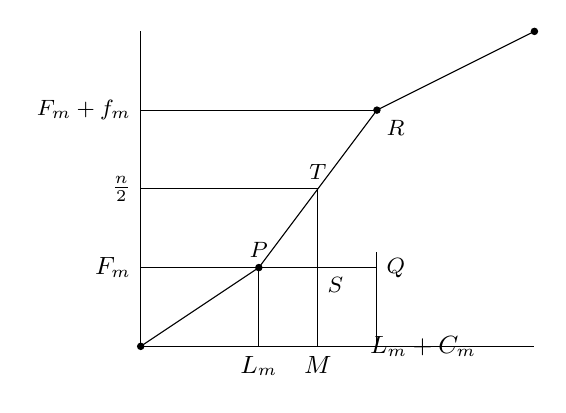
\begin{tikzpicture}
      \draw (0,0) -- (5,0);
      \draw (0,0) -- (0,4);
      \draw (0,0) -- (1.5, 1) -- (3, 3) -- (5, 4);
      \filldraw (0, 0) circle (0.04);
      \filldraw (1.5, 1) circle (0.04);
      \filldraw (3, 3) circle (0.04);
      \filldraw (5, 4) circle (0.04);
      \draw (0, 3) -- (3, 3);
      \draw (0, 2) -- (2.25, 2) -- (2.25, 0);
      \draw (1.5, 0) -- (1.5, 1) -- (0, 1);
      \draw (1.5, 1) -- (3, 1);
      \draw (3, 0) -- (3, 1.2);
      \draw (3, 1) node [right] {\footnotesize{${Q}$}};
      \draw (2.25, 1) node [below right] {\footnotesize{${S}$}};
      \draw (1.5, 1) node [above] {\footnotesize{${P}$}};
      \draw (2.25, 2) node [above] {\footnotesize{${T}$}};
      \draw (3, 3) node [below right] {\footnotesize{${R}$}};
      \draw (0, 3) node [left] {\footnotesize{$F_m + f_m$}};
      \draw (0, 2) node [left] {\small{$\frac{n}{2}$}};
      \draw (0, 1) node [left] {\small{$F_m$}};
      \draw (1.5, 0) node [below] {\small{$L_m$}};
      \draw (2.25, 0) node [below] {\small{$M$}};
      \draw (3, 0) node [below=8pt, right=-6pt] {\small{$L_m + C_m$}};
    \end{tikzpicture}
  \end{center}

  Diagram above shows a part of a cumulative frequency polygon, where $R$ is the
  point corresponding to the group containing the median, $P$ is the point
  corresponding to the group before the group containing the median, and $M$ is
  the median. Since $\Delta PQR \sim \Delta PST$,
  \begin{flalign*}
    \therefore \frac{PS}{PQ}             & = \frac{ST}{QR}                 \\
    \text{That is, } \frac{M - L_m}{C_m} & = \frac{\frac{n}{2} - F_m}{f_m}
  \end{flalign*}
  We get the following after simplifying the equation:
  \begin{cequation}
    M = L_m + \left(\frac{\frac{n}{2} - F_m}{f_m}\right)C_m
  \end{cequation}

  \subsection{Practice 4}

  \begin{enumerate}
    \item 10 workers in a factory made the same type of product in a day, the number of products made are as follows:
          \begin{flalign*}
            15 & \qquad 17 \qquad 14 \qquad 10 \qquad 15 \\
            19 & \qquad 17 \qquad 16 \qquad 14 \qquad 12
          \end{flalign*}
          Find the median of the number of products made by these 10 workers.
          \sol{}

          Sort the dataset:
          \begin{cequation}
            10 \quad 12 \quad 14 \quad 14 \quad 15 \quad 15 \quad 16 \quad 17 \quad 17 \quad 19
          \end{cequation}

          The median is the mean of the number in $\frac{10}{2} = 5$ and $\frac{10}{2}+1
            = 6$ position, which is $\frac{15 + 15}{2} = 15$.

    \item The table below shows the result of a right eye vision test for 49 students in
          a class:
          \begin{center}
            \begin{tabular}{|c|c|}
              \hline
              Vision & Number of Students \\
              \hline
              0.2    & 2                  \\
              0.3    & 3                  \\
              0.4    & 4                  \\
              0.5    & 3                  \\
              0.6    & 4                  \\
              0.8    & 9                  \\
              1.0    & 9                  \\
              1.2    & 10                 \\
              1.5    & 5                  \\
              \hline
            \end{tabular}
          \end{center}
          Find the median of the right eye vision of these students.
          \sol{}
          \begin{center}
            \begin{tabular}{|c|c|c|}
              \hline
              Vision & Number of Students & Cum. Frequency \\
              \hline
              0.2    & 2                  & 2              \\
              0.3    & 3                  & 5              \\
              0.4    & 4                  & 9              \\
              0.5    & 3                  & 12             \\
              0.6    & 4                  & 16             \\
              0.8    & 9                  & 25             \\\

              1.0    & 9                  & 34             \\
              1.2    & 10                 & 44             \\
              1.5    & 5                  & 49             \\
              \hline
            \end{tabular}
          \end{center}
          Since $n = 49$ is odd, the median is the number in the $\frac{49 + 1}{2} = 25$ position, which is $0.8$.

    \item The table below shows time distribution of 21 students browsing the Internet:
          \begin{center}
            \begin{tabular}{|c|c|}
              \hline
              Time (hours) & Number of Students \\
              \hline
              1.1 - 1.3    & 4                  \\
              1.4 - 1.6    & 3                  \\
              1.7 - 1.9    & 5                  \\
              2.0 - 2.2    & 4                  \\
              2.3 - 2.5    & 5                  \\
              \hline
            \end{tabular}
          \end{center}
          Find the median of the time distribution of these students.
          \sol{}
          \begin{center}
            \begin{tabular}{|c|c|c|}
              \hline
              Time      & Freq. & Cum. Freq. \\
              \hline
              1.1 - 1.3 & 4     & 4          \\
              1.4 - 1.6 & 3     & 7          \\
              1.7 - 1.9 & 5     & 12         \\
              2.0 - 2.2 & 4     & 16         \\
              2.3 - 2.5 & 5     & 21         \\
              \hline
            \end{tabular}
          \end{center}
          The median is the number in the $\frac{21}{2} = 10.5$ position, which is $1.7 - 1.9$.
          $C_m = 0.3$, $L_m = 1.65$, and $f_m = 5$, $F_m = 7$.
          \begin{flalign*}
            \therefore\ \textit{Mean} = 1.65 + \frac{10.5 - 7}{5} \cdot 0.3 = 1.86
          \end{flalign*}
  \end{enumerate}

  \subsection{Exercise 18.3b}

  \begin{enumerate}
    \item During a gymnastic competition, there are four judges scoring the performance
          of each contestant, and the median of these four scores are taken as the final
          score of the contestant. Given that the scores given by four judges are $9.5$,
          $9.4$, $9.8$, and $9.4$ respectively, find the final score of the contestant.
          \sol{}

          Sort the scores:
          \begin{cequation}
            9.4 \quad 9.4 \quad 9.5 \quad 9.8
          \end{cequation}
          The median is the mean of the number in $\frac{4}{2} = 2$ and $\frac{4}{2}+1 = 3$ position, which is $\frac{9.4 + 9.5}{2} = 9.45$.

    \item Following are the weight of 15 boys with same age:
          \begin{flalign*}
            36 & \qquad 35 \qquad 33 \qquad 37 \qquad 35 \\
            42 & \qquad 40 \qquad 38 \qquad 38 \qquad 39 \\
            40 & \qquad 41 \qquad 36 \qquad 38 \qquad 37
          \end{flalign*}
          \begin{enumerate}
            \item Find the median of these 15 boys. \sol{}

                  Sort the data:
                  \begin{flalign*}
                    33 & \quad 35 \quad 35 \quad 36 \quad 36 \quad 37 \quad 37 \quad 38 \quad 38 \quad 38 & \\
                    39 & \quad 40 \quad 41 \quad 42 \quad 43
                  \end{flalign*}
                  The median is the mean of the number in $\frac{15+1}{2} = 8$ position, which is $38$.

            \item Group the data using pattern $33 - 35$, $35 - 37$, $\ldots$, $41 - 43$. Then,
                  find the median. \sol{}
                  \begin{center}
                    \begin{tabular}{|c|c|c|}
                      \hline
                      Weight ($kg$) & Frequency & Cum. Frequency \\
                      \hline
                      33 - 35       & 1         & 1              \\
                      35 - 37       & 4         & 5              \\
                      37 - 39       & 5         & 10             \\
                      39 - 41       & 2         & 12             \\
                      41 - 43       & 2         & 14             \\
                      43 - 45       & 1         & 15             \\
                      \hline
                    \end{tabular}
                  \end{center}
                  The median is the number in the $\frac{15}{2} = 7.5$ position.
                  $C_m = 2$, $L_m = 37$, $f_m = 5$, and $F_m = 5$.
                  \begin{flalign*}
                    \therefore\ \textit{Median} = 37 + \frac{7.5 - 5}{5} \cdot 2 = 38
                  \end{flalign*}
          \end{enumerate}
    \item The table below shows the score distribution of a group of pupils in a minor
          test:
          \begin{center}
            \begin{tabular}{|c|c|}
              \hline
              Score & Number of Pupils \\
              \hline
              5     & 4                \\
              10    & 2                \\
              15    & 3                \\
              20    & $x$              \\
              25    & 4                \\
              \hline
            \end{tabular}
          \end{center}
          Assume that the median is 15, find the possibility value of $x$.
          \sol{}
          \begin{center}
            \begin{tabular}{|c|c|c|}
              \hline
              Score & Freq. & Cum. Freq. \\
              \hline
              5     & 4     & 4          \\
              10    & 2     & 6          \\
              15    & 3     & 9          \\
              20    & $x$   & 9 + x      \\
              25    & 4     & 13 + x     \\
              \hline
            \end{tabular}
          \end{center}
          \begin{flalign*}
            \frac{13 + x + 1}{2} & \leq 9     \\
            14 + x               & \leq 18    \\
            x                    & \leq 4     \\
            \therefore\ 0 \leq   & \ x \leq 4
          \end{flalign*}
          Therefore, the possibility values of $x$ are 0, 1, 2, 3, and 4.

    \item The following table shows the income of employees in a company:
          \begin{center}
            \begin{tabular}{|c|c|}
              \hline
              Income ($\$$) & Number of Employees \\
              \hline
              1000 - 2000   & 11                  \\
              2000 - 3000   & 17                  \\
              3000 - 4000   & 20                  \\
              4000 - 5000   & 10                  \\
              5000 - 6000   & 2                   \\
              \hline
            \end{tabular}
          \end{center}
          \begin{enumerate}
            \item Find the median of their income using cumulative frequency polygon. \sol{}
                  \begin{center}
                    \begin{tabular}{|c|c|c|}
                      \hline
                      Income ($\$$) & Freq. & Cum. Freq. \\
                      \hline
                      1000 - 2000   & 11    & 11         \\
                      2000 - 3000   & 17    & 28         \\
                      3000 - 4000   & 20    & 48         \\
                      4000 - 5000   & 10    & 58         \\
                      5000 - 6000   & 2     & 60         \\
                      \hline
                    \end{tabular}
                  \end{center}
                  The median is the number in $\frac{60}{2} = 30$ position.
                  \begin{center}
                    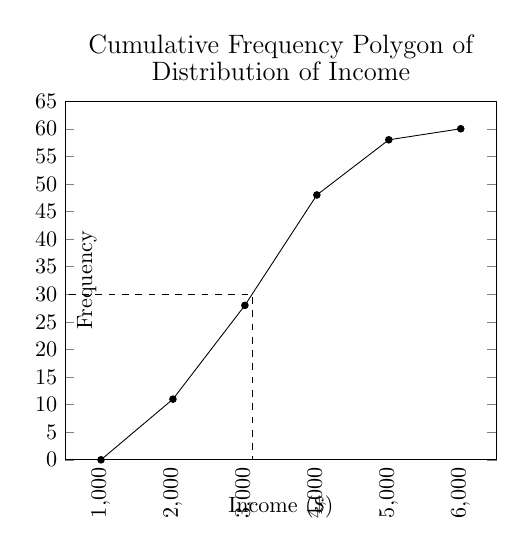
\begin{tikzpicture}[scale=0.8]
                      \begin{axis}[
                        title style = {align = center},
                        title={\large{Cumulative Frequency Polygon of} \\ \large{Distribution of Income}},
                        ymin=0, ymax=65,
                        ytick={0, 5, ..., 65},
                        xtick style={draw=none, fill=none, font=\footnotesize}, x tick label style =
                          {rotate=90,anchor=east}, xlabel=Income ($\$$), ylabel=Frequency, xlabel
                        style={at={(axis description cs:0.5, -0.08)}, anchor=north}, ylabel
                        style={at={(axis description cs:0.05, 0.5)}, anchor=center}, ] \addplot[forget
                          plot, sharp plot, mark=*, mark size=1.5pt, mark options={solid, fill=black,
                              draw=black}, draw=black] coordinates { (1000, 0) (2000, 11) (3000, 28) (4000, 48) (5000, 58) (6000, 60) };
                        \draw [dashed] (axis cs:0, 30) -- (axis cs:3100, 30) -- (axis cs:3100, 0);
                      \end{axis}
                    \end{tikzpicture}
                  \end{center}
                  Therefore, the median of their income is $\$3100$.

            \item Find the median of their income using formula and compare the result with (a).
                  \sol{}

                  The median is the number in the $\frac{60}{2} = 30$ position, which is $3000 -
                    4000$. $C_m = 1000$, $L_m = 3000$, and $f_m = 20$, $F_m = 28$.
                  \begin{cequation}
                    \therefore\ \textit{Median} = 3000 + \frac{30 - 28}{20} \cdot 1000 = 3100
                  \end{cequation}
                  Therefore, the median of their income is $\$3100$, which is the same as (a).
          \end{enumerate}

    \item The table below shows the distribution of height of 20 students:
          \begin{center}
            \begin{tabular}{|c|c|}
              \hline
              Height (cm) & Number of Students \\
              \hline
              120 - 130   & 3                  \\
              130 - 140   & 4                  \\
              140 - 150   & $x$                \\
              150 - 160   & 5                  \\
              160 - 170   & 6                  \\
              \hline
            \end{tabular}
          \end{center}
          Find:
          \begin{enumerate}
            \item The value of $x$. \sol{}
                  \begin{flalign*}
                    x + 3 + 4 + 5 + 6 & = 20      \\
                    x                 & = 20 - 18 \\
                                      & = 2
                  \end{flalign*}

            \item The median of their height. \sol{}
                  \begin{center}
                    \begin{tabular}{|c|c|c|}
                      \hline
                      Height $(cm)$ & Freq. & Cum. Freq. \\
                      \hline
                      120 - 130     & 3     & 3          \\
                      130 - 140     & 4     & 7          \\
                      140 - 150     & 2     & 9          \\
                      150 - 160     & 5     & 14         \\
                      160 - 170     & 6     & 20         \\
                      \hline
                    \end{tabular}
                  \end{center}
                  The median is the number in $\frac{20}{2} = 10$ position, which is $150 - 160$.
                  $C_m = 10$, $L_m = 150$, $f_m = 5$, and $F_m = 9$.
                  \begin{cequation}
                    \therefore\ \textit{Median} = 150 + \frac{10 - 9}{5} \cdot 10 = 152
                  \end{cequation}
                  Therefore, the median of their height is $152cm$.
          \end{enumerate}

    \item The table below shows the distribution of wages of workers in a factory:
          \begin{center}
            \begin{tabular}{|c|c|}
              \hline
              Wages $\$$ & Number of Workers \\
              \hline
              40 - 49    & 4                 \\
              50 - 59    & 14                \\
              60 - 69    & 5                 \\
              70 - 79    & $x$               \\
              80 - 89    & 2                 \\
              \hline
            \end{tabular}
          \end{center}
          Given that the median is $63.5$, find the value of $x$.
          \sol{}
          \begin{center}
            \begin{tabular}{|c|c|c|}
              \hline
              Wages $\$$ & Freq. & Cum. Freq. \\
              \hline
              40 - 49    & 4     & 4          \\
              50 - 59    & 14    & 18         \\
              60 - 69    & 5     & 23         \\
              70 - 79    & x     & 23 + x     \\
              80 - 89    & 2     & 25 + x     \\
              \hline
            \end{tabular}
          \end{center}

          $63.5$ is in between $60 - 69$, which is in the $\frac{25 + x}{2}$ position. $C_m = 10$, $L_m = 59.5$, $f_m = 5$, $F_m = 18$.
          \begin{flalign*}
            59.5 + \frac{\frac{25 + x}{2} - 18}{5} \cdot 10 & = 63.5 \\
            \frac{\frac{25 + x}{2} - 18}{5} \cdot 10        & = 4    \\
            \frac{\frac{25 + x}{2} - 18}{5}                 & = 0.4  \\
            \frac{25 + x}{2} - 18                           & = 2    \\
            \frac{25 + x}{2}                                & = 20   \\
            25 + x                                          & = 40   \\
            x                                               & = 15
          \end{flalign*}
  \end{enumerate}

  \subsection*{Mode}

  In a set of data, the mode is the value that occurs most frequently. There can
  be more than one mode in a set of data. If all the values in a dataset occur
  with the same frequency, then there is no mode for the data.

  For grouped data, the mode is the class that has the highest frequency, and
  there can be more than one mode. Besides that, the mode can also be estimated
  using histogram. The method is as follows:

  \begin{center}
    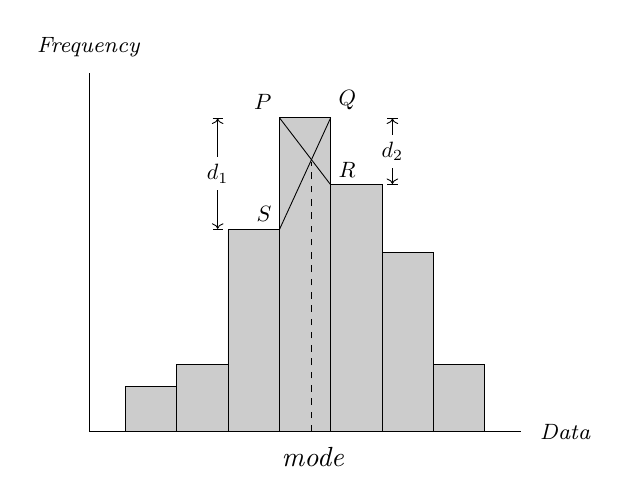
\begin{tikzpicture}[scale=0.8]
      \begin{axis}[
          ymin=0, ymax=16,
          ticks=none,
          ybar interval,
          grid=none,
          xtick style={draw=none},
          axis x line*=bottom,
          axis y line*=left,
        ]
        \addplot[draw=black, style={fill=gray!40},mark=no] plot coordinates { (0, 2) (1, 3) (2, 9) (3, 14) (4, 11) (5, 8) (6, 3) (7, 0) };
        \draw (axis cs:3, 9) -- (axis cs:4, 14);
        \draw (axis cs:3, 14) -- (axis cs:4, 11);
        \draw [dashed] (axis cs:3.63, 0) -- (axis cs: 3.63, 12);
        \node at (axis cs:3, 9) [above left] {$S$};
        \node at (axis cs:4, 14) [above right] {$Q$};
        \node at (axis cs:3, 14) [above left] {$P$};
        \node at (axis cs:4, 11) [above right] {$R$};
        \draw [|<->|] (axis cs:1.8, 9) -- (axis cs: 1.8, 14) node [midway, fill=white] {$d_1$};
        \draw [|<->|] (axis cs:5.2, 11) -- (axis cs: 5.2, 14) node [midway, fill=white] {$d_2$};
      \end{axis}
      \node at (3.55, -0.4) {$\textit{mode}$};
      \node at (7, 0) [right] {\footnotesize{\textit{Data}}};
      \node at (0, 5.8) [above] {\footnotesize{\textit{Frequency}}};
    \end{tikzpicture}
  \end{center}

  The diagram above shows a histogram of a set of data. The class corresponding
  to the highest rectangle is the mode of the data, and the mode is the x-value
  of the intersection point of $PR$ and $QS$.

  Unlike median, the formula of mode can be derived from similar triangles. Let:
  \begin{flalign*}
    L   & \text{ be the lower boundaries of the modal class}      \\
    C   & \text{ be the range of the modal class}                 \\
    d_1 & \text{ be the difference between the lower boundary of} \\
        & \text{ the modal class and the lower boundary of the}   \\
        & \text{ class immediately before the modal class}        \\
    d_2 & \text{ be the difference between the lower boundary of} \\
        & \text{ the modal class and the lower boundary of the}   \\
        & \text{ class immediately after the modal class}
  \end{flalign*}
  then
  \begin{cequation}
    \textit{mode} = L + \left(\frac{d_1}{d_1 + d_2}\right)C
  \end{cequation}

  \subsection{Practice 5}

  The following table shows the distribution of the score of 36 students in a
  Mathematics exam:
  \begin{center}
    \begin{tabular}{|c|c|}
      \hline
      Score   & Number of Students \\
      \hline
      20 - 29 & 2                  \\
      30 - 39 & 6                  \\
      40 - 49 & 10                 \\
      50 - 59 & 12                 \\
      60 - 69 & 3                  \\
      70 - 79 & 2                  \\
      80 - 89 & 1                  \\
      \hline
    \end{tabular}
  \end{center}
  \begin{enumerate}[label=(\alph*)]
    \item Find the modal class. \sol{}

          The modal class is $50 - 59$, which has the highest frequency of 12.

    \item Find the mode of score of the students using histogram. \sol{}
          \begin{center}
            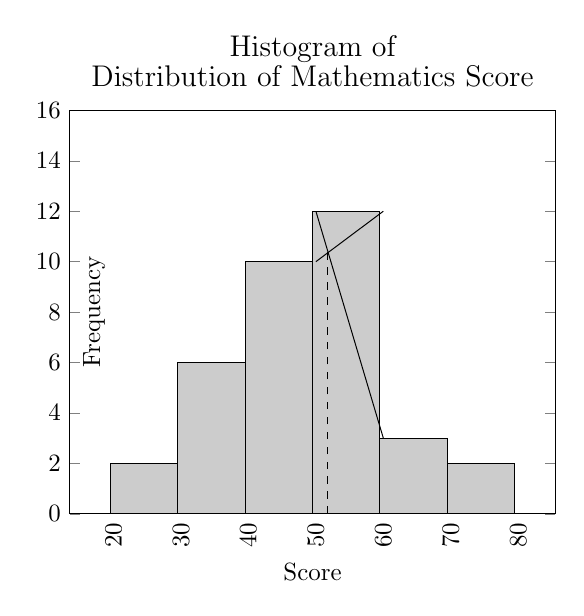
\begin{tikzpicture}[scale=0.9]
              \begin{axis}[
                  title style = {align = center},
                  title={\large{Histogram of} \\ \large{Distribution of Mathematics Score}},
                  ymin=0, ymax=16,
                  ytick={0, 2, ..., 16},
                  grid=none,
                  xtick style={draw=none, fill=none, font=\footnotesize},
                  x tick label style = {rotate=90,anchor=east},
                  xlabel=Score, ylabel=Frequency,
                  xlabel style={at={(axis description cs:0.5, -0.1)}, anchor=north},
                  ylabel style={at={(axis description cs:0.05, 0.5)}, anchor=center},
                ]
                \addplot[ybar interval, draw=black, style={fill=gray!40},mark=no] plot coordinates { (19.5, 2) (29.5, 6) (39.5, 10) (49.5, 12) (59.5, 3) (69.5, 2) (79.5, 1) };
                \draw (axis cs:50, 10) -- (axis cs:60, 12);
                \draw (axis cs:50, 12) -- (axis cs:60, 3);
                \draw [dashed] (axis cs:51.7, 0) -- (axis cs: 51.7, 10.5);
              \end{axis}
            \end{tikzpicture}
          \end{center}

          The mode of score of the students is approximately $51.5$.

    \item Find the mode of score of the students using formula. \sol{}

          $L = 49.5$, $C = 10$, $d_1 = 12 - 10 = 2$, $d_2 = 12 - 3 = 9$.
          \begin{flalign*}
            \therefore\ \textit{Mode} = 49.5 + \left(\frac{2}{2 + 9}\right)10 = 51.32
          \end{flalign*}

  \end{enumerate}

  \subsection*{Comparing mean, median and mode}

  Generally, the mean, median and mode of a set of data are all dirrent, and they
  are used to describe the data in different ways.

  \subsection{Exercise 18.3c}

  \begin{enumerate}
    \item Find the mode of the following data:
          \begin{enumerate}
            \item $3 \quad 4 \quad 3 \quad 2 \quad 4 \quad 5 \quad 5 \quad 5 \quad 4 \quad 4$
                  \sol{}

                  The mode is $4$, which has the highest frequency of 4.

            \item $7 \quad 6 \quad 8 \quad 8 \quad 5 \quad 6 \quad 6 \quad 9 \quad 8 \quad 5$
                  \sol{}

                  The mode is $6$ and $8$, which has the highest frequency of 3.

            \item $1.0 \quad 1.1 \quad 1.0 \quad 0.9 \quad 0.8 \quad 1.2 \quad 1.0 \quad 0.9 \quad 1.1 \quad$\\
                  $1.0$
                  \sol{}

                  The mode is $1.0$, which has the highest frequency of 4.
          \end{enumerate}
    \item In the sport competition of a high school, the scores of 17 athletes
          participating in men's high jump are as follows:
          \begin{center}
            \begin{tabular}{|c|c|}
              \hline
              Scores ($m$) & Number of Athletes \\ \hline
              1.50         & 2                  \\
              1.60         & 3                  \\
              1.65         & 2                  \\
              1.70         & 3                  \\
              1.75         & 4                  \\
              1.80         & 1                  \\
              1.85         & 1                  \\
              1.90         & 1                  \\
              \hline
            \end{tabular}
          \end{center}
          Find the mean, median and mode of their scores.
          \sol{}
          \begin{flalign*}
            \textit{Mean} & = \frac{1.50 \cdot 2 + 1.60 \cdot 3 + \cdots + 1.90 \cdot 1}{17} & \\
                          & = \frac{3 + 4.8 + 3.3 + 5.1 + 7 + 1.8 + 1.85 + 1.9}{17}            \\
                          & = \frac{28.75}{17}                                                 \\
                          & = 1.69m
          \end{flalign*}
          \begin{center}
            \begin{tabular}{|c|c|c|}
              \hline
              Scores ($m$) & No. of Athletes & Cum. Frequency \\ \hline
              1.50         & 2               & 2              \\
              1.60         & 3               & 5              \\
              1.65         & 2               & 7              \\
              1.70         & 3               & 10             \\
              1.75         & 4               & 14             \\
              1.80         & 1               & 15             \\
              1.85         & 1               & 16             \\
              1.90         & 1               & 17             \\
              \hline
            \end{tabular}
          \end{center}
          The median is the number at $\frac{17 + 1}{2} = 9$th position, which is $1.70m$.

          The mode is $1.75m$, which has the highest frequency of 4.

    \item In a Mathematics competition, the scores and the number of students who
          obtained the scores are as follows:
          \begin{center}
            \begin{tabular}{|c|c|}
              \hline
              Scores ($\%$) & Number of Students \\ \hline
              10 - 19       & 20                 \\
              20 - 29       & 60                 \\
              30 - 39       & 80                 \\
              40 - 49       & 40                 \\
              50 - 59       & 10                 \\
              \hline
            \end{tabular}
          \end{center}
          Find the modal class and the mode.
          \sol{}

          The modal clsas is $30 - 39$, which has the highest frequency of 80.

          $L = 29.5$, $C = 10$, $d_1 = 80 - 60 = 20$, $d_2 = 80 - 40 = 40$.
          \begin{flalign*}
            \therefore\ \textit{Mode} = 29.5 + \left(\frac{20}{20 + 40}\right)10 = 32.83
          \end{flalign*}

    \item Given that the mean of a dataset 3, 5, 8, 6, 8, 10, 5, 3, $x$, $y$ is 6,
          \begin{enumerate}
            \item Prove that $x+y = 12$ \prooff{}
                  \begin{flalign*}
                    \frac{3 + 5 + 8 + 6 + 8 + 10 + 5 + 3 + x + y}{10} & = 6  & \\
                    48 + x + y                                        & = 60   \\
                    x + y                                             & = 12
                  \end{flalign*}
            \item With that, if the following conditions are satisfied, find the mode of the
                  dataset.
                  \begin{enumerate}
                    \item $x = y$
                          \sol{}
                          \begin{flalign*}
                            x   & = y  \\
                            x+y & = 12 \\
                            2x  & = 12 \\
                            x   & = 6  \\
                            y   & = 6
                          \end{flalign*}
                          $\therefore$ The dataset becomes $3, 5, 8, 6, 8, 10, 5, 3, 6, 6$.
                          $\therefore$ The mode is $6$, which has the highest frequency of 3.
                    \item $x < y$
                          \sol{}
                          \begin{flalign*}
                            x   & < y  \\
                            x+y & = 12 \\
                            2x  & < 12 \\
                            x   & < 6  \\
                            y   & > 6
                          \end{flalign*}
                          When $x = 1$, $y = 11$, the dataset becomes $3, 5, 8, 6, 8, 10, 5, 3, 1, 11$.

                          $\therefore$ The mode are 3, 5, 8, which has the highest frequency of 2.

                          When $x = 2$, $y = 10$, the dataset becomes $3, 5, 8, 6, 8, 10, 5, 3, 2, 10$.

                          $\therefore$ The mode are 3, 5, 8, 10, which has the highest frequency of 2.

                          When $x = 3$, $y = 9$, the dataset becomes $3, 5, 8, 6, 8, 10, 5, 3, 3, 9$.

                          $\therefore$ The mode is 3, which has the highest frequency of 3.

                          When $x = 4$, $y = 8$, the dataset becomes $3, 5, 8, 6, 8, 10, 5, 3, 4, 8$.

                          $\therefore$ The mode is 8, which has the highest frequency of 3.

                          When $x = 5$, $y = 7$, the dataset becomes $3, 5, 8, 6, 8, 10, 5, 3, 5, 7$.

                          $\therefore$ The mode is 5, which has the highest frequency of 3.
                  \end{enumerate}

          \end{enumerate}

    \item The mean of a set of data 13, 5, 5, $n$, 5, 10, 10, 11, 9, $n^2$ is $7.4$,
          \begin{enumerate}
            \item Find the possible values of $n$. \sol{}
                  \begin{flalign*}
                    \frac{13 + 5 + 5 + n + \cdots + n^2}{10} & = 7.4 & \\
                    68 + n + n^2                             & = 74    \\
                    n^2 + n - 6                              & = 0     \\
                    (n + 3)(n - 2)                           & = 0     \\
                    n = -3 \text{ or } n                     & = 2
                  \end{flalign*}

            \item With that, if the following conditions are satisfied, find the median of the
                  dataset.
                  \begin{enumerate}
                    \item $n > 0$
                          \sol{}

                          If $n > 0$, $n = 2$, the dataset becomes 13, 5, 5, 2, 5, 10, 10, 11, 9, 4.
                          Rearranging the dataset, we get 2, 4, 5, 5, 5, 9, 10, 10, 11, 13. There are a
                          total of 10 elements in the dataset, so the median is the average of the
                          $\frac{10}{2} = 5$th and $\frac{10}{2} + 1 = 6$th elements, which is
                          $\frac{5+9}{2} = 7$.

                    \item $n < 0$
                          \sol{}

                          If $n < 0$, $n = -3$, the dataset becomes 13, 5, 5, -3, 5, 10, 10, 11, 9, 9.
                          Rearranging the dataset, we get -3, 5, 5, 5, 9, 9, 10, 10, 11, 13. There are a
                          total of 10 elements in the dataset, so the median is the average of the
                          $\frac{10}{2} = 5$th and $\frac{10}{2} + 1 = 6$th elements, which is
                          $\frac{9+9}{2} = 9$.
                  \end{enumerate}
          \end{enumerate}

    \item The following table shows the distribution of scores of a group of students in
          a competition:
          \begin{center}
            \begin{tabular}{|c|c|}
              \hline
              Scores & Number of Students \\ \hline
              0      & 3                  \\
              1      & x                  \\
              2      & 4                  \\
              3      & 6                  \\
              4      & 2                  \\
              \hline
            \end{tabular}
          \end{center}
          \begin{enumerate}
            \item Assume that the mode is 1, find the minimum value of $x$. \sol{}

                  Given that the \textbf{only} mode is 1, $x > 6$. Therefore, the minimum value
                  of $x$ is 7.

            \item Assume that the median is 2, find the maximum value of $x$. \sol{}

                  Construct a cumulative frequency table:
                  \begin{center}
                    \begin{tabular}{|c|c|c|}
                      \hline
                      Scores & Number of Students & Cum. Freq. \\ \hline
                      0      & 3                  & 3          \\
                      1      & $x$                & $3 + x$    \\
                      2      & 4                  & $7 + x$    \\
                      3      & 6                  & $13 + x$   \\
                      4      & 2                  & $15 + x$   \\
                      \hline
                    \end{tabular}
                  \end{center}
                  \begin{flalign*}
                    \frac{15 + x}{2} & > 3 + x  \\
                    15 + x           & > 6 + 2x \\
                    x                & < 9      \\
                    x                & = 8
                  \end{flalign*}

            \item Assume that the mean is $1.95$, find the value of $x$. \sol{}

                  \begin{center}
                    \begin{tabular}{|c|c|c|}
                      \hline
                      $x_i$ & $f_i$               & $f_i x_i$              \\
                      \hline
                      0     & 3                   & 0                      \\
                      1     & $x$                 & $x$                    \\
                      2     & 4                   & 8                      \\
                      3     & 6                   & 18                     \\
                      4     & 2                   & 8                      \\
                      \hline
                            & $\sum f_i = 15 + x$ & $\sum = f_i x_i34 + x$ \\
                      \hline
                    \end{tabular}
                  \end{center}
                  \begin{flalign*}
                    \frac{34 + x}{15 + x} & = 1.95          \\
                    34 + x                & = 29.25 + 1.95x \\
                    0.95x                 & = 4.75          \\
                    x                     & = 5
                  \end{flalign*}

          \end{enumerate}
    \item Given thet the mode, median and mean of 5 positive integers are 9, 8, and $7.6$
          respectively, find these 5 numbers. \sol{}

          Let the 5 numbers be $a, b, c, d, e$, arranged in ascending order.

          Since the median is 8, and $c$ is the middle of these 5 numbers, $c = 8$.

          Since the mode is 9, there must be more than 1 number that is 9. Since $9 > 8$,
          $d = e = 9$.

          Since the mean is $7.6$,
          \begin{flalign*}
            \frac{a + b + c + d + e}{5} & = 7.6 \\
            \frac{a + b + 8 + 9 + 9}{5} & = 7.6 \\
            a + b + 26                  & = 38  \\
            a + b                       & = 12
          \end{flalign*}
          Since the numbers are arranged in ascending order, and there is only one mode, $a < b < c$, that is, $a < b < 8$.
          \begin{flalign*}
            a + b         & = 12             \\
            a             & = 12 - b         \\
            \\
            a             & < b          < 8 \\
            12 - b        & < b     < 8      \\
            \\
            12            & < 2b             \\
            b             & < 8              \\
            \\
            b             & > 6              \\
            b             & < 8              \\
            6             & < b         < 8  \\
            \\
            \therefore\ b & = 7              \\
            a             & = 12 - 7 = 5
          \end{flalign*}
          Therefore, the 5 numbers are 5, 7, 8, 9, 9.

    \item The following table shows the amount of sales of a brand of shoes in a month:
          \begin{center}
            \begin{tabular}{|c|c|}
              \hline
              Shoes Number & Amount of Sales \\ \hline
              5            & 4               \\
              6            & 10              \\
              7            & 11              \\
              8            & 18              \\
              9            & 2               \\
              \hline
            \end{tabular}
          \end{center}
          \begin{enumerate}
            \item Find the mean, median, and mode. \sol{}

                  \begin{center}
                    \begin{tabular}{|c|c|c|}
                      \hline
                      $x_i$ & $f_i$           & $f_i x_i$            \\ \hline
                      5     & 4               & 20                   \\
                      6     & 10              & 60                   \\
                      7     & 11              & 77                   \\
                      8     & 18              & 144                  \\
                      9     & 2               & 18                   \\
                      \hline
                            & $\sum f_i = 45$ & $\sum f_i x_i = 319$ \\
                      \hline
                    \end{tabular}
                  \end{center}
                  \begin{flalign*}
                    \text{Mean} & = \frac{319}{45} = 7.09
                  \end{flalign*}
                  \begin{center}
                    \begin{tabular}{|c|c|c|}
                      \hline
                      Shoes Number & Sales & Cum. Freq. \\ \hline
                      5            & 4     & 4          \\
                      6            & 10    & 14         \\
                      7            & 11    & 25         \\
                      8            & 18    & 43         \\
                      9            & 2     & 45         \\
                      \hline
                    \end{tabular}
                  \end{center}
                  Since $n = 45$, the median is the number at the $23^{rd}$ position.
                  \begin{flalign*}
                    \text{Median} & = 7
                  \end{flalign*}
                  Since the number with the highest frequency of 18 is 8,
                  \begin{flalign*}
                    \text{Mode} & = 8
                  \end{flalign*}

                  $\therefore$ mean $= 7.09$, median $= 7$, mode $= 8$.

            \item Which of the following central tendency represents the data best? Why? \sol{}

                  The \textbf{mode} is the best central tendency to represent the data because it
                  is the number with the highest frequency, which is 18, and it is the shoes
                  number that most of the shoes are sold.
          \end{enumerate}
    \item In between 54 examinees in an exam, 15 of them come from cities, 39 of them
          come from suburbs. Below are the frequency distribution table of their scores:
          \begin{center}
            \begin{tabular}{|c|c|c|}
              \hline
              Scores   & City & Suburb \\ \hline
              12 - 23  & 0    & 1      \\
              23 - 34  & 0    & 0      \\
              34 - 45  & 0    & 5      \\
              45 - 56  & 1    & 6      \\
              56 - 67  & 3    & 5      \\
              67 - 78  & 4    & 13     \\
              78 - 89  & 6    & 4      \\
              89 - 100 & 1    & 5      \\
              \hline
            \end{tabular}
          \end{center}
          \begin{enumerate}
            \item Find the mean, median, and mode of the scores of the examinees from cities and
                  suburbs respectively. \sol{}

                  For the scores of the examinees from cities:
                  \begin{center}
                    \begin{tabular}{|c|c|c|c|}
                      \hline
                      Score    & Mid. $x_i$ & Freq. $f_i$     & $f_i x_i$ \\ \hline
                      12 - 23  & 17.5       & 0               & 0         \\
                      23 - 34  & 28.5       & 0               & 0         \\
                      34 - 45  & 39.5       & 0               & 0         \\
                      45 - 56  & 50.5       & 1               & 50.5      \\
                      56 - 67  & 61.5       & 3               & 184.5     \\
                      67 - 78  & 72.5       & 4               & 290       \\
                      78 - 89  & 83.5       & 6               & 501       \\
                      89 - 100 & 94.5       & 1               & 94.5      \\
                      \hline
                               &            & $\sum f_i = 15$ & $ 1120.5$ \\
                      \hline
                    \end{tabular}
                  \end{center}
                  \begin{flalign*}
                    \text{Mean} & = \frac{1120.5}{15} = 74.7
                  \end{flalign*}
                  \begin{center}
                    \begin{tabular}{|c|c|c|c|}
                      \hline
                      Score    & Feq. & Lower Than & Cum. Freq. \\ \hline
                      12 - 23  & 0    & 23         & 0          \\
                      23 - 34  & 0    & 34         & 0          \\
                      34 - 45  & 0    & 45         & 0          \\
                      45 - 56  & 1    & 56         & 1          \\
                      56 - 67  & 3    & 67         & 4          \\
                      67 - 78  & 4    & 78         & 8          \\
                      78 - 89  & 6    & 89         & 14         \\
                      89 - 100 & 1    & 100        & 15         \\
                      \hline
                    \end{tabular}
                  \end{center}
                  $n$ = 15, $\frac{n}{2} = 7.5$, the group of scores that contains the median is $67 - 78$, $C_m = 11$, $L_m = 67$, $f_m = 3$, $F_m = 4$,
                  \begin{flalign*}
                    \text{Median} & = 67 + \frac{7.5 - 4}{4} \cdot 11 = 76.63
                  \end{flalign*}
                  Since the modal class is $78 - 89$ with the highest frequency of 6, $C = 11$, $d_1 = 6 - 4 = 2$, $d_2 = 6 - 1 = 5$, $L_m = 78$,
                  \begin{flalign*}
                    \text{Mode} & = 78 + \frac{2}{2 + 5} \cdot 11 = 81.14
                  \end{flalign*}

                  $\therefore$ mean $= 74.7$, median $= 76.63$, mode $= 81.14$.

                  For the scores of the examinees from suburbs:
                  \begin{center}
                    \begin{tabular}{|c|c|c|c|}
                      \hline
                      Score    & Mid. $x_i$ & Freq. $f_i$     & $f_i x_i$ \\ \hline
                      12 - 23  & 17.5       & 1               & 17.5      \\
                      23 - 34  & 28.5       & 0               & 0         \\
                      34 - 45  & 39.5       & 5               & 197.5     \\
                      45 - 56  & 50.5       & 6               & 303       \\
                      56 - 67  & 61.5       & 5               & 307.5     \\
                      67 - 78  & 72.5       & 13              & 942.5     \\
                      78 - 89  & 83.5       & 4               & 334       \\
                      89 - 100 & 94.5       & 5               & 472.5     \\
                      \hline
                               &            & $\sum f_i = 39$ & $ 2574.5$ \\
                      \hline
                    \end{tabular}
                  \end{center}
                  \begin{flalign*}
                    \text{Mean} & = \frac{2574.5}{39} = 66.01
                  \end{flalign*}
                  \begin{center}
                    \begin{tabular}{|c|c|c|c|}
                      \hline
                      Score    & Feq. & Lower Than & Cum. Freq. \\ \hline
                      12 - 23  & 1    & 23         & 1          \\
                      23 - 34  & 0    & 34         & 1          \\
                      34 - 45  & 5    & 45         & 6          \\
                      45 - 56  & 6    & 56         & 12         \\
                      56 - 67  & 5    & 67         & 17         \\
                      67 - 78  & 13   & 78         & 30         \\
                      78 - 89  & 4    & 89         & 34         \\
                      89 - 100 & 5    & 100        & 39         \\
                      \hline
                    \end{tabular}
                  \end{center}
                  $n$ = 39, $\frac{n}{2} = 19.5$, the group of scores that contains the median is $67 - 78$, $C_m = 11$, $L_m = 67$, $f_m = 13$, $F_m = 17$,
                  \begin{flalign*}
                    \text{Median} & = 67 + \frac{19.5 - 17}{13} \cdot 11 = 69.12
                  \end{flalign*}
                  Since the modal class is $67 - 78$ with the highest frequency of 13, $C= 11$, $d_1 = 13 - 5 = 8$, $d_2 = 13 - 4 = 9$, $L = 67$,
                  \begin{flalign*}
                    \text{Mode} & = 67 + \frac{8}{8 + 9} \cdot 11 = 72.18
                  \end{flalign*}
                  $\therefore$ mean $= 66.01$, median $= 69.12$, mode $= 72.18$.

                  Therefore, the mean, median and mode of the scores are:
                  \begin{center}
                    \begin{tabular}{|c|c|c|}
                      \hline
                                    & City  & Suburbs \\ \hline
                      \text{Mean}   & 74.7  & 66.01   \\
                      \text{Median} & 76.63 & 69.12   \\
                      \text{Mode}   & 81.14 & 72.18   \\
                      \hline
                    \end{tabular}
                  \end{center}

            \item Find the mean, median and mode of the scores of all the examinees. \sol{}

                  \begin{center}
                    \begin{tabular}{|c|c|c|c|}
                      \hline
                      Score    & Mid. $x_i$ & Freq. $f_i$     & $f_i x_i$ \\ \hline
                      12 - 23  & 17.5       & 1               & 17.5      \\
                      23 - 34  & 28.5       & 0               & 0         \\
                      34 - 45  & 39.5       & 5               & 197.5     \\
                      45 - 56  & 50.5       & 7               & 353.5     \\
                      56 - 67  & 61.5       & 8               & 492       \\
                      67 - 78  & 72.5       & 17              & 1232.5    \\
                      78 - 89  & 83.5       & 10              & 835       \\
                      89 - 100 & 94.5       & 6               & 567       \\
                      \hline
                               &            & $\sum f_i = 54$ & $ 3695$   \\
                      \hline
                    \end{tabular}
                  \end{center}
                  \begin{flalign*}
                    \text{Mean} & = \frac{3695}{54} = 68.43
                  \end{flalign*}
                  \begin{center}
                    \begin{tabular}{|c|c|c|c|}
                      \hline
                      Score    & Feq. & Lower Than & Cum. Freq. \\ \hline
                      12 - 23  & 1    & 23         & 1          \\
                      23 - 34  & 0    & 34         & 1          \\
                      34 - 45  & 5    & 45         & 6          \\
                      45 - 56  & 7    & 56         & 13         \\
                      56 - 67  & 8    & 67         & 21         \\
                      67 - 78  & 17   & 78         & 38         \\
                      78 - 89  & 10   & 89         & 48         \\
                      89 - 100 & 6    & 100        & 54         \\
                      \hline
                    \end{tabular}
                  \end{center}
                  $n$ = 54, $\frac{n}{2} = 27$, the group of scores that contains the median is $67 - 78$, $C_m = 11$, $L_m = 67$, $f_m = 17$, $F_m = 21$,
                  \begin{flalign*}
                    \text{Median} & = 67 + \frac{27 - 21}{17} \cdot 11 = 70.88
                  \end{flalign*}
                  Since the modal class is $67 - 78$ with the highest frequency of 17, $C = 11$, $d_1 = 17 - 8 = 9$, $d_2 = 17 - 10 = 7$, $L = 67$,
                  \begin{flalign*}
                    \text{Mode} & = 67 + \frac{9}{9 + 7} \cdot 11 = 73.19
                  \end{flalign*}
          \end{enumerate}

    \item The following table shows the distribution of scores of a group of students in
          a Chinese language test:
          \begin{center}
            \begin{tabular}{|c|c|}
              \hline
              Scores $x$       & Number of Students \\ \hline
              $40 < x \leq 50$ & 12                 \\
              $50 < x \leq 60$ & 30                 \\
              $60 < x \leq 70$ & 35                 \\
              $70 < x \leq 80$ & 25                 \\
              $80 < x \leq 90$ & 10                 \\
              $9 < x \leq 100$ & 3                  \\
              \hline
            \end{tabular}
          \end{center}
          Find:
          \begin{enumerate}
            \item Mean. \sol{}
                  \begin{center}
                    \begin{tabular}{|c|c|c|c|}
                      \hline
                      Scores $x$        & Mid. $x_i$ & Freq. $f_i$      & $f_i x_i$ \\ \hline
                      $40 < x \leq 50$  & 45         & 12               & 540       \\
                      $50 < x \leq 60$  & 55         & 30               & 1650      \\
                      $60 < x \leq 70$  & 65         & 35               & 2275      \\
                      $70 < x \leq 80$  & 75         & 25               & 1875      \\
                      $80 < x \leq 90$  & 85         & 10               & 850       \\
                      $90 < x \leq 100$ & 95         & 3                & 285       \\
                      \hline
                                        &            & $\sum f_i = 115$ & $ 7475$   \\
                      \hline
                    \end{tabular}
                    \begin{flalign*}
                      \text{Mean} & = \frac{7475}{115} = 65
                    \end{flalign*}
                  \end{center}

            \item Modal class and mode. \sol{}

                  The modal class is $60 < x \leq 70$ with the highest frequency of 35, $C = 10$,
                  $d_1 = 35 - 30 = 5$, $d_2 = 35 - 25 = 10$, $L = 60$,
                  \begin{flalign*}
                    \text{Mode} & = 60 + \frac{5}{5 + 10} \cdot 10 = 63.33
                  \end{flalign*}

            \item Median. \sol{}
                  \begin{center}
                    \begin{tabular}{|c|c|c|c|}
                      \hline
                      Score             & Freq. & Lower Than & Cum. Freq. \\ \hline
                      $40 < x \leq 50$  & 12    & 50         & 12         \\
                      $50 < x \leq 60$  & 30    & 60         & 42         \\
                      $60 < x \leq 70$  & 35    & 70         & 77         \\
                      $70 < x \leq 80$  & 25    & 80         & 102        \\
                      $80 < x \leq 90$  & 10    & 90         & 112        \\
                      $90 < x \leq 100$ & 3     & 100        & 115        \\
                      \hline
                    \end{tabular}
                  \end{center}
                  $n$ = 115, $\frac{n}{2} = 57.5$, the group of scores that contains the median is $60 < x \leq 70$, $C_m = 10$, $L_m = 60$, $f_m = 35$, $F_m = 42$,
                  \begin{flalign*}
                    \text{Median} & = 60 + \frac{57.5 - 42}{35} \cdot 10 = 64.43
                  \end{flalign*}
          \end{enumerate}
  \end{enumerate}

  \section{Measures of Dispersion}

  The measures of dispersion can be used to describe the spread of the data.

  When we're describing a set of data, if we only use the mean, the information
  provided by the dataset is not enough. For example, given the mean, median, and
  mode of the average marks of four students in a Mathematics test are all 70
  marks, we can't tell the difference between the four students. Their marks
  might be similar (e.g. 68, 72, 70, 70) or they might be very different (e.g.
  100, 40, 70, 70). The latter case is obviously more spread out than the former
  case.

  The most common measures of dispersion are range, interquartile range, quartile
  deviation, standard deviation, mean deviation, variance, and standard
  deviation.

  \subsection*{Range}

  The range of a set of data is the difference between the largest and the
  smallest value in the dataset.

  For grouped data, the range is the difference between the upper limit of the
  highest class and the lower limit of the lowest class.

  \subsection*{Quartile, Interquartile Range, and Quartile Deviation}

  Quartiles are three value $Q_1$, $Q_2$, and $Q_3$ that divide a dataset into
  four equal parts. $Q_2$ is the median of the dataset. $Q_1$ and $Q_3$ are the
  medians of the two halves of the dataset, called the lower quartile and the
  upper quartile respectively.

  Assume that the number of data in a sorted dataset is $n$. If $n$ is odd, then

  When $n$ is even, split the dataset into two halves, with $n/2$ data in each
  half.

  When $n$ is odd, split the data into two halves after removing the median, with
  $(n-1)/2$ data in each half.

  The median of the lower half is $Q_1$ and the median of the upper half is
  $Q_3$.

  For grouped data, we can make a cumulative frequency polygon. In the percentage
  of the polygon,

  $25\%$ of the data is below $Q_1$.

  $50\%$ of the data is below $Q_2$.

  $75\%$ of the data is below $Q_3$.

  Using the same method of deriving the formula for median, we can derive the
  formula for upper and lower quartiles. Let
  \begin{flalign*}
    n   & \text{ be the number of data in the dataset, aka } \sum f_i \\
    L_k & \text{ be the lower boundaries of the class of } Q_k        \\
    C_k & \text{ be the class range of the class of } Q_k             \\
    f_k & \text{ be the frequency of the class of } Q_k               \\
    F_k & \text{ be the cumulative frequency of the class of } Q_k    \\
  \end{flalign*}
  then
  \begin{cequation}
    Q_1 = L_1 + \left(\frac{\frac{n}{4} - F_1}{f_1}\right)C_1
  \end{cequation}
  \begin{cequation}
    Q_2 = L_2 + \left(\frac{\frac{3n}{4} - F_2}{f_2}\right)C_2
  \end{cequation}

  The difference between the upper and lower quartiles is called the
  interquartile range. That is,
  \begin{cequation}
    \textit{Interquartile range} = Q_3 - Q_1
  \end{cequation}

  The quartile deviation is the interquartile range divided by 2, written as
  $Q.D.$, that is,
  \begin{cequation}
    \textit{Q.D.} = \frac{Q_3 - Q_1}{2}
  \end{cequation}

  Since the interquartile range and the quartile deviation are not affected by
  the outliers, they are more robust than the range, and are more suitable for
  representing the spread of the data.

  \subsection{Practice 6}

  \begin{enumerate}
    \item Find the range, quartiles and interquartile range of the following data:
          \begin{enumerate}
            \item 4 \quad 8 \quad 7 \quad 3 \quad 3 \quad 9 \quad 6 \quad 5 \quad 1 \quad 1 \quad 2
                  \sol{}

                  Sorting the data, we get
                  \[1 \quad 1 \quad \typel{2}{$Q_1 = 2$} \quad 3 \quad 3 \quad \typel{4}{$Q_2 = 4$} \quad 5 \quad 6 \quad \typel{7}{$Q_3 = 7$} \quad 8 \quad 9\]

                  The range is $9 - 1 = 8$.

                  The interquartile range is $Q.D. = 7 - 2 = 5$.

            \item 7 \quad 6 \quad 8 \quad 8 \quad 5 \quad 6 \quad 1 \quad 9 \quad 8
                  \sol{}

                  Sorting the data, we get
                  \[1 \typel{\quad 5 \quad 6 \quad}{$Q_1 = \frac{5 + 6}{2} = 5.5$} 6 \typem{\quad 7 \quad}{$Q_2 = 7$} 8 \typel{\quad 8 \quad 8 \quad}{$Q_3 = \frac{8 + 8}{2} = 8$} 9\]

                  The range is $9 - 1 = 8$.

                  The interquartile range is $8 - 5.5 = 2.5$.

            \item 1.0 \quad 1.1 \quad 1.5 \quad 0.7 \quad 0.8 \quad 1.2 \quad 1.4\ \quad 0.9 \quad 1.6 \quad 1.3
                  \sol{}

                  Sorting the data, we get
                  \[0.7 \quad 0.8 \quad \typel{0.9}{$Q_1 = 0.9$} \quad 1.0 \typem{ \quad 1.1 \quad 1.2 \quad }{$Q_2 = \frac{1.1 + 1.2}{2} = 1.15$} 1.3 \quad \typel{1.4}{$Q_3 = 1.4$} \quad 1.5 \quad 1.6\]

                  The range is $1.6 - 0.7 = 0.9$.

                  The interquartile range is $1.4 - 0.9 = 0.5$.

            \item 3 \quad 4 \quad 7 \quad 2 \quad 4 \quad 6 \quad 5 \quad 8
                  \sol{}

                  Sorting the data, we get
                  \[2 \qquad \typel{3 \qquad 4}{$Q_1 = \frac{3 + 4}{2} = 3.5$} \qquad \typem{ 4 \qquad 5}{$Q_2 = \frac{4 +5}{2} = 4.5$} \qquad \typel{6 \qquad 7}{$Q_2 = \frac{6 + 7}{2} = 6.5$} \qquad 8\]

                  The range is $8 - 2 = 6$.

                  The interquartile range is $6.5 - 3.5 = 3$.
          \end{enumerate}

    \item The table below shows the cumulative frequency distribution table of the
          heights of 60 students:
          \begin{center}
            \begin{tabular}{|c|c|}
              \hline
              Height ($cm$) & Cumulative Frequency \\
              \hline
              150-155       & 3                    \\
              155-160       & 10                   \\
              160-165       & 22                   \\
              165-170       & 37                   \\
              170-175       & 51                   \\
              175-180       & 58                   \\
              180-185       & 60                   \\
              \hline
            \end{tabular}
          \end{center}
          \begin{enumerate}
            \item Find the interquartile range of the heights of the students from the cumulative
                  frequency polygon. \sol{}
                  \begin{center}
                    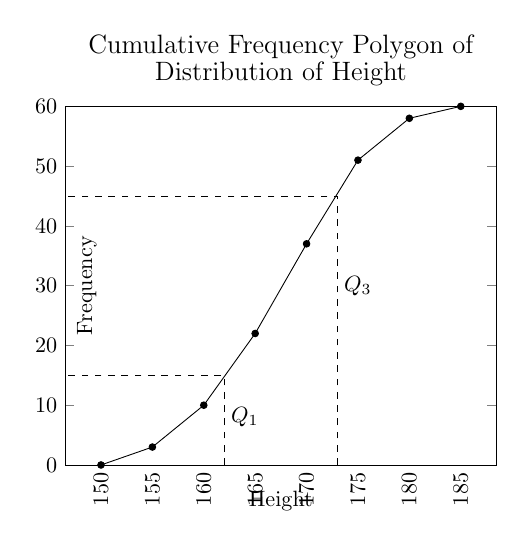
\begin{tikzpicture}[scale=0.8]
                      \begin{axis}[
                          title style = {align = center},
                          title={\large{Cumulative Frequency Polygon of} \\ \large{Distribution of Height}},
                          ymin=0, ymax=60,
                          ytick={0, 10, ..., 60},
                          xtick={150, 155, ..., 185},
                          xtick style={draw=none, fill=none, font=\footnotesize}, x tick label style =
                            {rotate=90,anchor=east}, xlabel=Height, ylabel=Frequency, xlabel style={at={(axis
                                  description cs:0.5, -0.05)}, anchor=north}, ylabel style={at={(axis
                                  description cs:0.05, 0.5)}, anchor=center}, ] \addplot[forget plot, sharp
                          plot, mark=*, mark size=1.5pt, mark options={solid, fill=black, draw=black},
                          draw=black] coordinates { (150, 0) (155, 3) (160, 10) (165, 22) (170, 37) (175, 51)
                            (180, 58) (185, 60) };
                        \draw [dashed] (axis cs: 162, 0) -- (axis cs: 162, 15) -- (axis cs: 0, 15);
                        \draw [dashed] (axis cs: 173, 0) -- (axis cs: 173, 45) -- (axis cs: 0, 45);
                        \node at (axis cs: 175, 30) {$Q_3$};
                        \node at (axis cs: 164, 8) {$Q_1$};
                      \end{axis}
                    \end{tikzpicture}
                  \end{center}
                  From the graph, $Q_1$ is approximately $162cm$ and $Q_3$ is approximately $173cm$. Hence,
                  \begin{flalign*}
                    Q.D. = \frac{173 - 162}{2} = 5.5
                  \end{flalign*}

            \item Find the interquartile range of the heights of the students using formula.
                  \sol{}

                  $n = 60$, $\frac{n}{4} = 15$, the class that contains $Q_1$ is $160-165$, $C_1 = 5$, $L_1 = 160$, $f_1 = 11$, $F_1 = 10$,
                  \begin{flalign*}
                    Q_1 = 160 + \frac{15 - 10}{12} \cdot 5 = 162.083
                  \end{flalign*}
                  $n = 60$, $\frac{3n}{4} = 45$, the class that contains $Q_3$ is $170-175$, $C_3 = 5$, $L_3 = 170$, $f_3 = 14$, $F_3 = 37$,
                  \begin{flalign*}
                    Q_3 = 170 + \frac{45 - 37}{14} \cdot 5 = 172.857
                  \end{flalign*}
                  Hence,
                  \begin{flalign*}
                    Q.D. = \frac{172.857 - 162.083}{2} = 5.39
                  \end{flalign*}
          \end{enumerate}
  \end{enumerate}

  \subsection{Exercise 18.4a}

  \begin{enumerate}
    \item Following are the sales of televisions of a shop in 11 days:
          \begin{flalign*}
            4 \quad 9 \quad 0 \quad 1 \quad 3 \quad 4 \quad 2 \quad 5 \quad 7 \quad 2 \quad 3
          \end{flalign*}
          Find:
          \begin{enumerate}
            \item The range. \sol{}

                  Rearranging the data,

                  \begin{flalign*}
                     & 0 \quad 1 \quad 2 \quad 2 \quad 3 \quad 3 \quad 4 \quad 4 \quad 5 \quad 7 \quad 9 &
                  \end{flalign*}
                  Hence, the range is $9 - 0 = 9$.

            \item The quartiles and interquartile range. \sol{}

                  Rearranging the data,
                  \begin{flalign*}
                     & 0 \quad 1 \quad \typel{2}{$Q_1 = 2$} \quad 2 \quad 3 \quad \typel{3}{$Q_2 = 3$} \quad 4 \quad 4 \quad \typel{5}{$Q_3 = 5$} \quad 7 \quad 9 &
                  \end{flalign*}
                  Hence, the interquartile range is $5 - 2 = 3$.
          \end{enumerate}

    \item Given a set of data: 1.2, 1.0, 1.1, 1.3, 1.5, 1.7, 1.2, 1.0. Find:
          \begin{enumerate}
            \item The range. \sol{}

                  Rearranging the data,
                  \begin{flalign*}
                     & 1.0 \quad 1.0 \quad 1.1 \quad 1.2 \quad 1.2 \quad 1.3 \quad 1.5 \quad 1.7 &
                  \end{flalign*}
                  Hence, the range is $1.7 - 1.0 = 0.7$.

            \item The quartiles and interquartile deviation. \sol{}

                  Rearranging the data,
                  \begin{flalign*}
                     & 1.0 \quad \typel{1.0 \quad 1.1}{$Q_1 = \frac{1.0}{1.1} = 1.05$} \quad \typem{1.2 \quad 1.2}{$Q_2 = \frac{1.2+1.2}{2} = 1.2$} \quad \typel{1.3 \quad 1.5}{$Q_3 = \frac{1.3 + 1.5}{2} = 1.4$} \quad 1.7 &
                  \end{flalign*}
                  Hence, the interquartile deviation is $\frac{1.4 - 1.05}{2} = 0.18$.
          \end{enumerate}

    \item The distribution of scores of Mathematics test of 100 senior 1 students from a
          high school are as follows:
          \begin{center}
            \begin{tabular}{|c|c|}
              \hline
              Scores   & Number of Students \\
              \hline
              30 - 40  & 3                  \\
              40 - 50  & 4                  \\
              50 - 60  & 13                 \\
              60 - 70  & 22                 \\
              70 - 80  & 30                 \\
              80 - 90  & 23                 \\
              90 - 100 & 5                  \\
              \hline
            \end{tabular}
          \end{center}
          Find the interquartile deviation of the scores.
          \sol{}
          \begin{center}
            \begin{tabular}{|c|c|c|c|}
              \hline
              Scores   & Freq. & Lower Than & Cumulative Freq. \\
              \hline
              30 - 40  & 3     & 40.5       & 3                \\
              40 - 50  & 4     & 50.5       & 7                \\
              50 - 60  & 13    & 60.5       & 20               \\
              60 - 70  & 22    & 70.5       & 42               \\
              70 - 80  & 30    & 80.5       & 72               \\
              80 - 90  & 23    & 90.5       & 95               \\
              90 - 100 & 5     & 100.5      & 100              \\
              \hline
            \end{tabular}
          \end{center}

          $n = 100$, $\frac{n}{4} = 25$, The class that contains the lower quartile is $60 - 70$, $C_1 = 10$, $L_1 = 60.5$, $f_1 = 22$, $F_1 = 20$,
          \begin{flalign*}
            Q_1 = 60.5 + \frac{25 - 20}{22} \cdot 10 = 62.773
          \end{flalign*}
          $n = 100$, $\frac{3n}{4} = 75$, The class that contains the upper quartile is $80 - 90$, $C_2 = 10$, $L_2 = 80.5$, $f_2 = 23$, $F_2 = 72$,
          \begin{flalign*}
            Q_3 = 80.5 + \frac{75 - 72}{23} \cdot 10 = 81.804
          \end{flalign*}
          Hence,
          \begin{flalign*}
            Q.D. = \frac{81.804 - 62.773}{2} = 9.52
          \end{flalign*}
  \end{enumerate}

  \subsubsection*{Mean Deviation}

  Let the mean of a set of data $x_1$, $x_2$, $\ldots$, $x_n$ be $\bar{x}$, $|x_i
    - \bar{x}|$ is the difference between the $i$th data and the mean, the mean of
  these $n$ differences are called the mean deviation, and can be used to
  calculate the measure of dispersion of the data. That is,
  \begin{cequation}
    \textit{Mean Deviation} = \frac{\sum |x_i - \bar{x}|}{n}
  \end{cequation}

  If the possible value given data are $x_1$, $x_2$, $\ldots$, $x_n$, their
  frequencies are $f_1$, $f_2$, $\ldots$, $f_n$, respectively, then the mean
  deviation can be calculated as follows:
  \begin{cequation}
    \textit{Mean Deviation} = \frac{\sum |x_i - \bar{x}|f_i}{\sum f_i}
  \end{cequation}

  For grouped data, we take the midpoints of the classes as the representative
  value $x_i$.

  \subsection{Practice 7}

  Complete the following table, and find the mean and mean deviation of the data.
  \begin{center}
    \begin{tabular}{|c|c|c|c|c|c|}
      \hline
      Lim.    & $f_i$ & Mid. $x_i$ & $f_ix_i$ & $|x_i - \bar{x}|$ & $|x_i - \bar{x}|f_i$ \\
      \hline
      50 - 54 & 2     &            &          &                   &                      \\
      55 - 59 & 3     &            &          &                   &                      \\
      60 - 64 & 6     &            &          &                   &                      \\
      65 - 69 & 9     &            &          &                   &                      \\
      \hline
    \end{tabular}
  \end{center}
  \sol{}
  \begin{center}
    \begin{tabular}{|c|c|c|c|c|c|}
      \hline
      Lim.    & $f_i$ & Mid. $x_i$ & $f_ix_i$ & $|x_i - \bar{x}|$ & $|x_i - \bar{x}|f_i$ \\
      \hline
      50 - 54 & 2     & 52         & 104      & 10.5              & 21                   \\
      55 - 59 & 3     & 57         & 171      & 5.5               & 16.5                 \\
      60 - 64 & 6     & 62         & 372      & 0.5               & 3                    \\
      65 - 69 & 9     & 67         & 603      & 4.5               & 40.5                 \\
      \hline
              & 20    &            & 1250     &                   & 81                   \\
      \hline
    \end{tabular}
  \end{center}
  \begin{flalign*}
    \bar{x}                 & = \frac{1250}{20} = 62.5 \\
    \textit{Mean Deviation} & = \frac{81}{20} = 4.05
  \end{flalign*}

  \subsection{Exercise 18.4b}

  \begin{enumerate}
    \item Find the mean deviation of the following dataset:
          \begin{enumerate}
            \item 7 \quad 10 \quad 9 \quad 12 \quad 4 \quad 11 \quad 3
                  \sol{}
                  \begin{flalign*}
                    \bar{x}            & = \frac{7 + 10 + 9 + 12 + 4 + 11 + 3}{7} = 8 & \\
                    \textit{Mean Dev.} & = \frac{1}{7}(|7 - 8| + \cdots + |3 - 8|)      \\
                                       & = 2.86
                  \end{flalign*}

            \item 58 \quad 65 \quad 38 \quad 76 \quad 43
                  \sol{}
                  \begin{flalign*}
                    \bar{x}            & = \frac{58 + 65 + 38 + 76 + 43}{5} = 56       & \\
                    \textit{Mean Dev.} & = \frac{1}{5}(|58 - 56| + \cdots + |43 - 56|)   \\
                                       & = 12.4
                  \end{flalign*}

            \item 45.0 \quad 46.5 \quad 47.0 \quad 48.0 \quad 48.7 \quad 48.9 \quad 49.5 \quad 50.4
                  \sol{}
                  \begin{flalign*}
                    \bar{x}         & = \frac{45.0 + 46.5 + \cdots + 50.4}{8} = 48          & \\
                    \textit{M Dev.} & = \frac{1}{8}(|45.0 - 48.3| + \cdots + |50.4 - 48.3|)   \\
                                    & = 1.38
                  \end{flalign*}
          \end{enumerate}

    \item The table below shows the frequency of the number of questions answered
          correctly by 26 students in a Mathematics minor test:
          \begin{center}
            \begin{tabular}{|c|c|}
              \hline
              Num. of Corr. Ans. Ques. & Num. of Stud. \\
              \hline
              1                        & 0             \\
              2                        & 1             \\
              3                        & 1             \\
              4                        & 1             \\
              5                        & 6             \\
              6                        & 8             \\
              7                        & 6             \\
              8                        & 1             \\
              9                        & 1             \\
              10                       & 1             \\
              \hline
            \end{tabular}
          \end{center}
          Find the mean deviation fo the number of questions answered correctly.
          \sol{}
          \begin{center}
            \begin{tabular}{|c|c|c|c|c|}
              \hline
              $x_i$ & $f_i$ & $f_ix_i$ & $|x_i - \bar{x}|$ & $|x_i - \bar{x}|f_i$ \\
              \hline
              1     & 0     & 0        & 5                 & 0                    \\
              2     & 1     & 2        & 4                 & 4                    \\
              3     & 1     & 3        & 3                 & 3                    \\
              4     & 1     & 4        & 2                 & 2                    \\
              5     & 6     & 30       & 1                 & 6                    \\
              6     & 8     & 48       & 0                 & 0                    \\
              7     & 6     & 42       & 1                 & 6                    \\
              8     & 1     & 8        & 2                 & 2                    \\
              9     & 1     & 9        & 3                 & 3                    \\
              10    & 1     & 10       & 4                 & 4                    \\
              \hline
                    & 26    &          &                   & 30                   \\
              \hline
            \end{tabular}
          \end{center}
          \begin{flalign*}
            \bar{x}                 & = \frac{156}{26} = 6   \\
            \textit{Mean Deviation} & = \frac{30}{26} = 1.15
          \end{flalign*}

    \item Following are the test scores of 36 students:
          \begin{flalign*}
            77 & \quad 60 \quad 52 \quad 73 \quad 60 \quad 50 \quad 70 \quad 60 \quad 52 & \\
            68 & \quad 59 \quad 50 \quad 72 \quad 59 \quad 48 \quad 66 \quad 58 \quad 46   \\
            60 & \quad 48 \quad 34 \quad 61 \quad 55 \quad 40 \quad 62 \quad 55 \quad 42   \\
            63 & \quad 55 \quad 43 \quad 65 \quad 56 \quad 45 \quad 65 \quad 57 \quad 46
          \end{flalign*}
          \begin{enumerate}
            \item Group the dataset above according to the pattern $[34 - 38)$, $[38 - 42)$, $[42
                    - 46)$, \ldots, then make a frequency distribution table. \sol{}
                  \begin{center}
                    \begin{tabular}{|c|c|}
                      \hline
                      Range            & Frequency \\
                      \hline
                      $34 \leq x < 38$ & 1         \\
                      $38 \leq x < 42$ & 1         \\
                      $42 \leq x < 46$ & 3         \\
                      $46 \leq x < 50$ & 4         \\
                      $50 \leq x < 54$ & 4         \\
                      $54 \leq x < 58$ & 5         \\
                      $58 \leq x < 62$ & 8         \\
                      $62 \leq x < 66$ & 4         \\
                      $66 \leq x < 70$ & 2         \\
                      $70 \leq x < 74$ & 3         \\
                      $74 \leq x < 78$ & 1         \\
                      \hline
                    \end{tabular}
                  \end{center}

            \item Find the mean from the frequency distribution table. \sol{}
                  \begin{center}
                    \begin{tabular}{|c|c|c|c|}
                      \hline
                      Range            & Mid $x_i$ & Freq. $f_i$ & $f_ix_i$ \\
                      \hline
                      $34 \leq x < 38$ & 36        & 1           & 36       \\
                      $38 \leq x < 42$ & 40        & 1           & 40       \\
                      $42 \leq x < 46$ & 44        & 3           & 132      \\
                      $46 \leq x < 50$ & 48        & 4           & 192      \\
                      $50 \leq x < 54$ & 52        & 4           & 208      \\
                      $54 \leq x < 58$ & 56        & 5           & 280      \\
                      $58 \leq x < 62$ & 60        & 8           & 480      \\
                      $62 \leq x < 66$ & 64        & 4           & 256      \\
                      $66 \leq x < 70$ & 68        & 2           & 136      \\
                      $70 \leq x < 74$ & 72        & 3           & 216      \\
                      $74 \leq x < 78$ & 76        & 1           & 76       \\
                      \hline
                                       &           & 36          & 2052     \\
                      \hline
                    \end{tabular}
                  \end{center}
                  \begin{flalign*}
                    \bar{x} = \frac{2052}{36} = 57
                  \end{flalign*}

            \item Find the mean deviation from the frequency distribution table. \sol{}
                  \begin{center}
                    \begin{tabular}{|c|c|c|c|}
                      \hline
                      $x_i$ & $f_i$ & $|x_i - \bar{x}|$ & $f_i|x_i - \bar{x}|$ \\
                      \hline
                      36    & 1     & 21                & 21                   \\
                      40    & 1     & 17                & 17                   \\
                      44    & 3     & 13                & 39                   \\
                      48    & 4     & 9                 & 36                   \\
                      52    & 4     & 5                 & 20                   \\
                      56    & 5     & 1                 & 5                    \\
                      60    & 8     & 3                 & 24                   \\
                      64    & 4     & 7                 & 28                   \\
                      68    & 2     & 11                & 22                   \\
                      72    & 3     & 15                & 45                   \\
                      76    & 1     & 19                & 19                   \\
                      \hline
                            & 36    & 107               & 276                  \\
                      \hline
                    \end{tabular}
                  \end{center}
                  \begin{flalign*}
                    \textit{Mean Deviation} = \frac{276}{36} = 7.67
                  \end{flalign*}
          \end{enumerate}
  \end{enumerate}

  \subsubsection*{Variance and Standard Deviation}

  Let the mean of a set of data $x_1$, $x_2$, $\ldots$, $x_n$ be $\bar{x}$,
  ${(x_1 - \bar{x})}^2$ be the square of the difference between the $i^{th}$ data
  and the mean, the square of the mean of these $n$ differences are called the
  variance, written as $\sigma^2$, that is,
  \begin{cequation}
    \sigma^2 = \frac{\sum (x_i - \bar{x})^2}{n}
  \end{cequation}

  The square root of the variance is called the standard deviation, written as
  $\sigma$, that is,
  \begin{cequation}
    \sigma = \sqrt{\frac{\sum (x_i - \bar{x})^2}{n}}
  \end{cequation}

  If the possible values of given data are $x_1$, $x_2$, $\ldots$, $x_n$, their
  frequencies are $f_1$, $f_2$, $\ldots$, $f_n$, respectively, then
  \begin{cequation}
    \sigma^2 = \frac{\sum (x_i - \bar{x})^2f_i}{\sum f_i}
  \end{cequation}
  \begin{cequation}
    \sigma = \sqrt{\frac{\sum (x_i - \bar{x})^2f_i}{\sum f_i}}
  \end{cequation}

  For grouped data, we take the midpoints of the classes as the representative
  value $x_i$.

  The above formula are a bit complicated, so we can simplify the formula:
  \begin{flalign*}
    \sigma^2 & = \frac{\sum (x_i - \bar{x})^2f_i}{\sum f_i}                                  \\
             & = \frac{\sum x_i^2 f_i - 2\bar{x}\sum x_i f_i + \sum \bar{x}^2 f_i}{\sum f_i} \\
             & = \frac{\sum x_i^2 f_i}{\sum f_i} - 2\bar{x}^2 + \bar{x}^2                    \\
             & = \frac{\sum x_i^2 f_i}{\sum f_i} - \bar{x}^2
  \end{flalign*}

  Hence, when the frequency of value $x_i$ is $f_i$, Then
  \begin{cequation}
    \sigma^2 = \frac{\sum x_i^2 f_i}{\sum f_i} - \bar{x}^2
  \end{cequation}
  \begin{cequation}
    \sigma = \sqrt{\frac{\sum x_i^2 f_i}{\sum f_i} - \bar{x}^2}
  \end{cequation}

  When all the frequencies $f_i$ are equal to $1$, then
  \begin{cequation}
    \sigma^2 = \frac{\sum x_i^2}{n} - \bar{x}^2
  \end{cequation}
  \begin{cequation}
    \sigma = \sqrt{\frac{\sum x_i^2}{n} - \bar{x}^2}
  \end{cequation}

  Compared to mean deviation, the variance and standard deviation do not contain
  absolute value, so it is more convenient to use them. Furthermore, the variance
  and standard deviation are more sensitive to the difference between the data
  and the mean, so they are more commonly used in daily life.

  \subsection{Practice 8}

  \begin{enumerate}
    \item Measuring the height of 10 plant seedlings (in $cm$) in a lab, we get the
          following data:
          \begin{flalign*}
            12 & \quad 6 \quad 15 \quad 3 \quad 12 \quad 6 \quad 21 \quad 15 \quad 18 \quad 12 &
          \end{flalign*}
          Find the standard deviation of the height of the plant seedlings.
          \sol{}
          \begin{flalign*}
            \bar{x}  & = \frac{12 + 6 + \cdots + 12}{10} = 12         \\
            \sigma^2 & = \frac{12^2 + 6^2 + \cdots + 12^2}{10} - 12^2 \\
                     & = \frac{1728}{10} - 144                        \\
                     & = 28.8                                         \\
            \sigma   & = \sqrt{28.8} = 5.37
          \end{flalign*}

    \item Complete the following table, then find the standard deviation.
          \begin{enumerate}
            \item \begin{tabular}{|c|c|c|c|}
                    \hline
                    $x_i$ & $f_i$ & $x_i f_i$ & $x_i^2 f_i$ \\
                    \hline
                    3     & 30    &           &             \\
                    5     & 35    &           &             \\
                    7     & 28    &           &             \\
                    \hline
                  \end{tabular}
                  \sol{}
                  \begin{center}
                    \resizebox{\columnwidth-5em}{!}{
                      \begin{tabular}{|c|c|c|c|}
                        \hline
                        $x_i$ & $f_i$           & $x_i f_i$            & $x_i^2 f_i$             \\
                        \hline
                        3     & 30              & 90                   & 270                     \\
                        5     & 35              & 175                  & 875                     \\
                        7     & 28              & 196                  & 1372                    \\
                        \hline
                              & $\sum f_i = 93$ & $\sum x_i f_i = 461$ & $\sum x_i^2 f_i = 2517$ \\
                        \hline
                      \end{tabular}
                    }
                  \end{center}
                  \begin{flalign*}
                    \bar{x}  & = \frac{461}{93} = 4.96    \\
                    \sigma^2 & = \frac{2517}{93} - 4.96^2 \\
                             & = 27.06 - 24.60            \\
                             & = 2.46                     \\
                    \sigma   & = \sqrt{2.46} = 1.57
                  \end{flalign*}

            \item \begin{tabular}{|c|c|c|c|c|}
                    \hline
                    Limit     & $f_i$ & $Mid. x_i$ & $x_i f_i$ & $x_i^2 f_i$ \\
                    \hline
                    150 - 154 & 5     &            &           &             \\
                    155 - 159 & 8     &            &           &             \\
                    160 - 164 & 10    &            &           &             \\
                    165 - 169 & 7     &            &           &             \\
                    170 - 174 & 6     &            &           &             \\
                    175 - 179 & 4     &            &           &             \\
                    \hline
                  \end{tabular}
                  \sol{}
                  \begin{center}
                    \resizebox{\columnwidth-4.4em}{!}{
                      \begin{tabular}{|c|c|c|c|c|}
                        \hline
                        Limit     & $f_i$           & $Mid. x_i$ & $x_i f_i$             & $x_i^2 f_i$                \\
                        \hline
                        150 - 154 & 5               & 152        & 760                   & 115520                     \\
                        155 - 159 & 8               & 157        & 1256                  & 197192                     \\
                        160 - 164 & 10              & 162        & 1620                  & 262440                     \\
                        165 - 169 & 7               & 167        & 1169                  & 195223                     \\
                        170 - 174 & 6               & 172        & 1032                  & 177504                     \\
                        175 - 179 & 4               & 177        & 708                   & 125316                     \\
                        \hline
                                  & $\sum f_i = 40$ &            & $\sum x_i f_i = 6545$ & $\sum x_i^2 f_i = 1073195$ \\
                        \hline
                      \end{tabular}
                    }
                  \end{center}
                  \begin{flalign*}
                    \bar{x}  & = \frac{6545}{40} = 163.625     \\
                    \sigma^2 & = \frac{1073195}{40} - 163.88^2 \\
                             & = 26829.88 - 26773.14           \\
                             & = 56.74                         \\
                    \sigma   & = \sqrt{55.74} = 7.53
                  \end{flalign*}
          \end{enumerate}
  \end{enumerate}

  \subsection{Exercise 18.4c}

  \begin{enumerate}
    \item Find the variance and standard deviation of the following dataset:
          \begin{enumerate}
            \item 3 \quad 6 \quad 3 \quad 8
                  \sol{}
                  \begin{flalign*}
                    \bar{x}  & = \frac{3 + 6 + 3 + 8}{4} = 5           \\
                    \sigma^2 & = \frac{3^2 + 6^2 + 3^2 + 8^2}{4} - 5^2 \\
                             & = 29.5 - 25                             \\
                             & = 4.5                                   \\
                    \sigma   & = \sqrt{4.5} = 2.12
                  \end{flalign*}

            \item 3 \quad 3 \quad 4 \quad 5 \quad 10
                  \sol{}
                  \begin{flalign*}
                    \bar{x}  & = \frac{3 + 3 + 4 + 5 + 10}{5} = 5             \\
                    \sigma^2 & = \frac{3^2 + 3^2 + 4^2 + 5^2 + 10^2}{5} - 5^2 \\
                             & = 31.8 - 25                                    \\
                             & = 6.8                                          \\
                    \sigma   & = \sqrt{6.8} = 2.61
                  \end{flalign*}

            \item 2 \quad 9 \quad 10 \quad 10 \quad 12 \quad 2 \quad 10 \quad 9
                  \sol{}
                  \begin{flalign*}
                    \bar{x}  & = \frac{2 + 9 + \cdots + 10 + 9}{8} = 8   \\
                    \sigma^2 & = \frac{2^2 + 9^2 + \dots + 9^2}{8} - 8^2 \\
                             & = 76.75 - 64                              \\
                             & = 12.75                                   \\
                    \sigma   & = \sqrt{12.75} = 3.57
                  \end{flalign*}
          \end{enumerate}

    \item Find the variance and standard deviation of the data:
          \begin{enumerate}
            \item \begin{tabular}{|c|c|}
                    \hline
                    Values & Frequency \\
                    \hline
                    6      & 35        \\
                    5      & 36        \\
                    4      & 30        \\
                    \hline
                  \end{tabular}
                  \sol{}
                  \begin{center}
                    \resizebox{\columnwidth-5em}{!}{
                      \begin{tabular}{|c|c|c|c|}
                        \hline
                        $x_i$ & $f_i$            & $x_i f_i$            & $x_i^2 f_i$             \\
                        \hline
                        6     & 35               & 210                  & 1260                    \\
                        5     & 36               & 180                  & 900                     \\
                        4     & 30               & 120                  & 480                     \\
                        \hline
                              & $\sum f_i = 101$ & $\sum x_i f_i = 510$ & $\sum x_i^2 f_i = 2640$ \\
                        \hline
                      \end{tabular}
                    }
                  \end{center}
                  \begin{flalign*}
                    \bar{x}  & = \frac{510}{101} = 5.05    \\
                    \sigma^2 & = \frac{2640}{101} - 5.05^2 \\
                             & = 26.14 - 25.5              \\
                             & = 0.64                      \\
                    \sigma   & = \sqrt{0.64} = 0.80
                  \end{flalign*}

            \item \begin{tabular}{|c|c|}
                    \hline
                    Values & Frequency \\
                    \hline
                    60     & 4         \\
                    70     & 6         \\
                    80     & 2         \\
                    90     & 5         \\
                    100    & 1         \\
                    \hline
                  \end{tabular}
                  \sol{}
                  \begin{center}
                    \resizebox{\columnwidth-4.6em}{!}{
                      \begin{tabular}{|c|c|c|c|}
                        \hline
                        $x_i$ & $f_i$           & $x_i f_i$             & $x_i^2 f_i$              \\
                        \hline
                        60    & 4               & 240                   & 14400                    \\
                        70    & 6               & 420                   & 29400                    \\
                        80    & 2               & 160                   & 12800                    \\
                        90    & 5               & 450                   & 40500                    \\
                        100   & 1               & 100                   & 10000                    \\
                        \hline
                              & $\sum f_i = 18$ & $\sum x_i f_i = 1370$ & $\sum x_i^2f_i = 107100$ \\
                        \hline
                      \end{tabular}
                    }
                  \end{center}
                  \begin{flalign*}
                    \bar{x}  & = \frac{1370}{18} = 76.11     \\
                    \sigma^2 & = \frac{107100}{18} - 76.11^2 \\
                             & = 5950 - 5792.90              \\
                             & = 157.10                      \\
                    \sigma   & = \sqrt{157.10} = 12.53
                  \end{flalign*}
          \end{enumerate}

    \item Given two sets of data:
          \begin{center}
            \begin{tabular}{|c|c|}
              \hline
              A    & B    \\
              \hline
              9.9  & 10.3 \\
              10.3 & 10   \\
              9.8  & 9.5  \\
              10.1 & 10.4 \\
              10.4 & 10.5 \\
              10   & 9.4  \\
              9.8  & 9.8  \\
              9.7  & 10.1 \\
              \hline
            \end{tabular}
          \end{center}
          Find the mean and variance of these two sets of data respectively, and state which set of data is more spread out.
          \sol{}

          For data $A$,
          \begin{flalign*}
            \bar{x}  & = \frac{9.9 + 10.3 + \cdots + 9.7}{8} = 10         \\
            \sigma^2 & = \frac{9.9^2 + 10.3^2 + \cdots + 9.7^2}{8} - 10^2 \\
                     & = 100.055 - 100                                    \\
                     & = 0.06
          \end{flalign*}
          For data $B$,
          \begin{flalign*}
            \bar{x}  & = \frac{10.3 + 10 + \cdots + 10.1}{8} = 10.0          \\
            \sigma^2 & = \frac{10.3^2 + 10^2 + \cdots + 10.1^2}{8} - 10.05^2 \\
                     & = 100.145 - 100                                       \\
                     & = 0.15
          \end{flalign*}
          Since $\sigma^2$ of data $B$ is larger than that of data $A$, data $B$ is more spread out.

    \item Given the Chinese language test scores of two groups of students are as
          follows:
          \begin{center}
            \begin{tabular}{|c|c|}
              \hline
              Group A & Group B \\
              \hline
              76      & 82      \\
              90      & 84      \\
              84      & 85      \\
              86      & 89      \\
              81      & 79      \\
              87      & 80      \\
              86      & 91      \\
              82      & 89      \\
              85      & 79      \\
              83      & 74      \\
              \hline
            \end{tabular}
          \end{center}
          Find the mean and standard deviation of these two sets of data respectively, and state which set of data is more centered.
          \sol{}

          For Group $A$,
          \begin{flalign*}
            \bar{x}  & = \frac{76 + 90 + \cdots + 83}{10} = 84         \\
            \sigma^2 & = \frac{76^2 + 90^2 + \cdots + 83^2}{10} - 84^2 \\
                     & = 7069.2 - 7056                                 \\
                     & = 13.2                                          \\
            \sigma   & = \sqrt{13.2} = 3.63
          \end{flalign*}
          For Group $B$,
          \begin{flalign*}
            \bar{x}  & = \frac{82 + 84 + \cdots + 74}{10} = 83.2         \\
            \sigma^2 & = \frac{82^2 + 84^2 + \cdots + 74^2}{10} - 83.2^2 \\
                     & = 6948.6 - 6922.24                                \\
                     & = 26.36                                           \\
            \sigma   & = \sqrt{26.36} = 5.13
          \end{flalign*}
          Since $\sigma$ of Group $A$ is smaller than that of Group $B$, Group $A$ is more centered.

    \item The table below shows the height distribution of all students of the same
          grade:
          \begin{center}
            \begin{tabular}{|c|c|}
              \hline
              Height ($cm$) & Frequency \\
              \hline
              145 - 149     & 10        \\
              150 - 154     & 36        \\
              155 - 159     & 193       \\
              160 - 164     & 205       \\
              165 - 169     & 240       \\
              170 - 174     & 83        \\
              175 - 179     & 33        \\
              \hline
            \end{tabular}
          \end{center}
          Find the mean and standard deviation of the height of all students of the same grade.
          \sol{}
          \begin{center}
            \resizebox{\columnwidth-3em}{!}{
              \begin{tabular}{|c|c|c|c|c|}
                \hline
                Range     & $x_i$ & $f_i$            & $x_if_i$                & $x_i^2f_i$                  \\
                \hline
                145 - 149 & 147   & 10               & 1470                    & 216090                      \\
                150 - 154 & 152   & 36               & 5472                    & 831744                      \\
                155 - 159 & 157   & 193              & 30301                   & 4757257                     \\
                160 - 164 & 162   & 205              & 33210                   & 5380020                     \\
                165 - 169 & 167   & 240              & 40080                   & 6693360                     \\
                170 - 174 & 172   & 83               & 14276                   & 2455472                     \\
                175 - 179 & 177   & 33               & 5841                    & 1033857                     \\
                \hline
                          &       & $\sum f_i = 800$ & $\sum f_i x_i = 130650$ & $\sum f_i x_i^2 = 21367800$ \\
                \hline
              \end{tabular}
            }
          \end{center}
          \begin{flalign*}
            \bar{x}  & = \frac{130650}{800} = 163.31cm   \\
            \sigma^2 & = \frac{21367800}{800} - 163.31^2 \\
                     & = 26709.75 - 26670.16             \\
                     & = 38.78cm                         \\
            \sigma   & = \sqrt{38.78} = 6.23cm
          \end{flalign*}

    \item Following are teh weight distribution of 100 students in a school:
          \begin{center}
            \begin{tabular}{|c|c|}
              \hline
              Weight ($kg$) & Number of Students \\
              \hline
              45 - 47       & 3                  \\
              48 - 50       & 16                 \\
              51 - 53       & 20                 \\
              54 - 56       & 32                 \\
              57 - 59       & 15                 \\
              60 - 62       & 10                 \\
              63 - 65       & 4                  \\
              \hline
            \end{tabular}
          \end{center}
          Find the variance and standard deviation.
          \sol{}
          \begin{center}
            \resizebox{\columnwidth-3em}{!}{
              \begin{tabular}{|c|c|c|c|c|}
                \hline
                Range   & $x_i$ & $f_i$            & $x_if_i$              & $x_i^2f_i$                \\
                \hline
                45 - 47 & 46    & 3                & 138                   & 6348                      \\
                48 - 50 & 49    & 16               & 784                   & 38416                     \\
                51 - 53 & 52    & 20               & 1040                  & 54080                     \\
                54 - 56 & 55    & 32               & 1760                  & 96800                     \\
                57 - 59 & 58    & 15               & 870                   & 50460                     \\
                60 - 62 & 61    & 10               & 610                   & 37210                     \\
                63 - 65 & 64    & 4                & 256                   & 16384                     \\
                \hline
                        &       & $\sum f_i = 100$ & $\sum f_i x_i = 5458$ & $\sum f_i x_i^2 = 299698$ \\
                \hline
              \end{tabular}
            }
          \end{center}
          \begin{flalign*}
            \bar{x}  & = \frac{5458}{100} = 54.58kg   \\
            \sigma^2 & = \frac{299698}{100} - 54.58^2 \\
                     & = 2996.98 - 2978.98            \\
                     & = 18.00kg                      \\
            \sigma   & = \sqrt{18.00} = 4.24kg
          \end{flalign*}

    \item Given the sum of 10 values is 400, and the sum of their square is 16400. Find
          the mean and variance of these 10 values. \sol{}
          \begin{flalign*}
            \bar{x}  & = \frac{400}{10} = 40     \\
            \sigma^2 & = \frac{16400}{10} - 40^2 \\
                     & = 1640 - 1600             \\
                     & = 40
          \end{flalign*}

    \item Given 30 values $x_1$, $x_2$, $\cdots$, $x_{30}$, the mean of these values is
          5, and the standard deviation is 2. Find $\sum\limits_{i=1}^{30} x_i$ and
          $\sum\limits_{i=1}^{30} x_i^2$. \sol{}
          \begin{flalign*}
            \bar{x}                               & = 5   \\
            \frac{\sum\limits_{i=1}^{30} x_i}{30} & = 5   \\
            \sum\limits_{i=1}^{30} x_i            & = 150 \\
          \end{flalign*}
          \begin{flalign*}
            \sigma                                        & = 2   \\
            \sigma^2                                      & = 4   \\
            \frac{\sum\limits_{i=1}^{30} x_i^2}{30} - 5^2 & = 4   \\
            \frac{\sum\limits_{i=1}^{30} x_i^2}{30}       & = 29  \\
            \sum\limits_{i=1}^{30} x_i^2                  & = 870
          \end{flalign*}

    \item The mean of 5 values is 10, and it remains the same after adding $p$ to
          dataset.
          \begin{enumerate}
            \item Find the value of $p$. \sol{}

                  Let the dataset be $x$.
                  \begin{flalign*}
                    \bar{x} = 10                                 \\
                    \frac{\sum\limits_{i=1}^{5} x_i}{5} = 10     \\
                    \sum\limits_{i=1}^{5} x_i = 50               \\
                    \frac{\sum\limits_{i=1}^{5} x_i + p}{6} = 10 \\
                    50 + p & = 60                                \\
                    p      & = 10
                  \end{flalign*}

            \item If the sum of square of 5 original values is 558, find the variance of the 6
                  values after adding $p$. \sol{}
                  \begin{flalign*}
                    \sigma^2 = \frac{\sum\limits_{i=1}^{5} x_i^2 + p^2}{6} - 10^2 \\
                    = \frac{558 + 100}{6} - 100                                   \\
                    = 109.67 - 100                                                \\
                    = 9.67
                  \end{flalign*}
          \end{enumerate}

    \item Given that the mean of 3, 6, 7, 8, 9, 12, 14, 15, $x$, $y$ is 13, standard
          deviation is $\sqrt{102}$, find the value of $x$ and $y$. \sol{}
          \begin{flalign*}
            \bar{x} = \frac{3+6+\cdots+15+x+y}{10} & = 13  \\
            \frac{74 + x + y}{10}                  & = 13  \\
            74 + x + y                             & = 130 \\
            x + y                                  & = 56
          \end{flalign*}
          \begin{flalign*}
            \sigma                                                  & = \sqrt{102} \\
            \sigma^2                                                & = 102        \\
            \frac{3^2 + 6^2 + \cdots + 15^2 + x^2 + y^2}{10} - 13^2 & = 102        \\
            \frac{804 + x^2 + y^2}{10} - 169                        & = 102        \\
            \frac{804 + x^2 + y^2}{10}                              & = 271        \\
            804 + x^2 + y^2                                         & = 2710       \\
            x^2 + y^2                                               & = 1906
          \end{flalign*}
          \setcounter{equation}{0}
          \begin{numcases}{}
            x + y = 56 \\
            x^2 + y^2 = 1906
          \end{numcases}
          \begin{flalign*}
            (1)                               \Rightarrow y                                   & = 56 - x & (1) \\
            \text{Sub } (1) \text{ into } (2)  \Rightarrow x^2 + (56-x)^2                     & = 1906         \\
            x^2 + x^2 - 112x + 3136                                                           & = 1906         \\
            2x^2 - 112x + 1230                                                                & = 0            \\
            x^2 - 56x + 615                                                                   & = 0            \\
            (x - 15)(x - 41)                                                                  & = 0            \\
            x                                                              = 15 \text{ or } x & = 41           \\
            \text{When } x = 15, y = 56 - 15                                                  & = 41           \\
            \text{When } x = 41, y = 56 - 41                                                  & = 15           \\
            \\
            \therefore\ \begin{cases}
                          x = 15 \\
                          y = 41
                        \end{cases} \text{ or } \begin{cases}
                                                  x = 41 \\
                                                  y = 15
                                                \end{cases}
          \end{flalign*}
  \end{enumerate}

  \section{Coefficient of Variation}

  Generally speaking, when we want to compare the variability of two or more sets
  of data, only comparing the standard deviation of each group is not enough. If
  the properties or the units of the data are different, the standard deviation
  of each group must not be comparable. For example, if we want to know whether
  the deviation of the height of students in a class is larger than that of the
  weight of students in the same class, we need a relative metric as the standard
  of comparison, and the coefficient of variation is such a metric. For a
  non-negative set of value, the definition of coefficient of variation is as
  follows:
  \begin{cequation}
    v = \frac{\sigma}{\bar{x}} \cdot 100\%
  \end{cequation}

  From the definition, we can see that the coefficient of variation the standard
  deviation when the mean is 1. Thus, when the coefficient of variation is large,
  it means that the variability of the data is large, and vice versa.

  \subsection{Practice 9}

  In a minor test, the full mark of Chinese language test for senior 2 students
  is 100, its average mark is 70, and the standard deviation is 10, while the
  full mark of Mathematics test is 70, its average mark is 40, and the standard
  deviation is 8. Compare the variability of the two tests. \sol{}
  \begin{flalign*}
    v_{\text{Chinese}} & = \frac{10}{70} \cdot 100\% = 14.29\% \\
    v_{\text{Math}}    & = \frac{8}{40} \cdot 100\% = 20\%
  \end{flalign*}
  $\because\ v_{\text{Math}} > v_{\text{Chinese}}$

  \noindent $\therefore$ Mathematics test is more variable than Chinese language test.

  \subsection{Exercise 18.5}

  \begin{enumerate}
    \item The statistics of the height and weight if grade 1 students in a primary school
          are as follows:
          \begin{center}
            \begin{tabular}{|c|c|c|}
              \hline
                            & Mean   & Standard Deviation \\
              \hline
              Height ($cm$) & 115.87 & 4.86               \\
              Weight ($cm$) & 19.39  & 2.16               \\
              \hline
            \end{tabular}
          \end{center}
          Compare the variability of the height and weight of the students.
          \sol{}
          \begin{flalign*}
            v_{\text{Height}} & = \frac{4.86}{115.87} \cdot 100\% = 4.19\% \\
            v_{\text{Weight}} & = \frac{2.16}{19.39} \cdot 100\% = 11.14\%
          \end{flalign*}
          $\because\ v_{\text{Weight}} > v_{\text{Height}}$

          \noindent $\therefore$ The weight of the students is more variable than their height.

    \item The table below shows the first semester Mathematics exam average mark and
          standard deviation of five junior 1 classes in a school:
          \begin{center}
            \begin{tabular}{|c|c|c|}
              \hline
              Class & Average Mark & Standard Deviation \\
              \hline
              A     & 62           & 11                 \\
              B     & 74           & 9                  \\
              C     & 65           & 10                 \\
              D     & 70           & 7                  \\
              E     & 53           & 8                  \\
              \hline
            \end{tabular}
          \end{center}
          Which class has the smallest coefficient of variation?
          \sol{}
          \begin{flalign*}
            v_{\text{A}} & = \frac{11}{62} \cdot 100\% = 17.74\% \\
            v_{\text{B}} & = \frac{9}{74} \cdot 100\% = 12.16\%  \\
            v_{\text{C}} & = \frac{10}{65} \cdot 100\% = 15.38\% \\
            v_{\text{D}} & = \frac{7}{70} \cdot 100\% = 10\%     \\
            v_{\text{E}} & = \frac{8}{53} \cdot 100\% = 15.09\%
          \end{flalign*}
          $\because\ v_{\text{D}} < v_{\text{B}} < v_{\text{A}} < v_{\text{C}} < v_{\text{E}}$

          $\therefore\ \text{Class D}$ has the smallest coefficient of variation.

    \item The table below shows the Mathematics exam results of two groups of students
          $A$ and $B$:
          \begin{center}
            \begin{tabular}{|c|c|}
              \hline
              Group & Marks                                  \\
              \hline
              A     & 60 \quad 98 \quad 76 \quad 84 \quad 52 \\
              B     & 88 \quad 58 \quad 90 \quad 69 \quad 78 \\
              \hline
            \end{tabular}
          \end{center}
          \begin{enumerate}
            \item Find the average mark of each group. \sol{}
                  \begin{flalign*}
                    \bar{x}_A & = \frac{60 + 98 + 76 + 84 + 52}{5} = 74   \\
                    \bar{x}_B & = \frac{88 + 58 + 90 + 69 + 78}{5} = 76.6
                  \end{flalign*}

            \item Find the standard deviation of each group. \sol{}
                  \begin{flalign*}
                    \sigma^2_A & = \frac{60^2 + \cdots + 52^2}{5} - 74^2 \\
                               & = 5748 - 5476                           \\
                               & = 272                                   \\
                    \sigma_A   & = \sqrt{272} = 16.49                    \\
                  \end{flalign*}
                  \begin{flalign*}
                    \sigma^2_B & = \frac{88^2 + \cdots + 78^2}{5} - 76.6^2 \\
                               & = 6010.6 - 5867.56                        \\
                               & = 143.04                                  \\
                    \sigma_B   & = \sqrt{143.04} = 11.96
                  \end{flalign*}
            \item Find the coefficient of variation of each group. \sol{}
                  \begin{flalign*}
                    v_A & = \frac{16.49}{74} \cdot 100\% = 22.28\%   \\
                    v_B & = \frac{11.96}{76.6} \cdot 100\% = 15.61\%
                  \end{flalign*}
          \end{enumerate}

    \item The table below shows the price of of papayas and grapes per kilogram in the
          first half of the year (in $\$$):
          \begin{center}
            \begin{tabular}{|c|c|c|}
              \hline
              Month    & Papaya & Grapes \\
              \hline
              January  & 3.50   & 20.00  \\
              February & 3.00   & 22.00  \\
              March    & 2.50   & 24.00  \\
              April    & 3.20   & 23.00  \\
              May      & 3.60   & 18.00  \\
              June     & 2.80   & 21.00  \\
              \hline
            \end{tabular}
          \end{center}
          \begin{enumerate}
            \item Find the average price and standard deviation of papayas and grapes
                  respectively in the first half of the year. \sol{}
                  \begin{flalign*}
                    \bar{x}_{\text{Papaya}} & = \frac{3.50 + \cdots + 2.80}{6} = 3.10 \\
                    \bar{x}_{\text{Grapes}} & = \frac{20 + \cdots + 21}{6} = 21.33
                  \end{flalign*}
                  \begin{flalign*}
                    \sigma^2_{\text{Papaya}} & = \frac{3.50^2 + \cdots + 2.80^2}{6} - 3.10^2 \\
                                             & = 9.77 - 9.61                                 \\
                                             & = 0.15                                        \\
                    \sigma_{\text{Papaya}}   & = \sqrt{0.15} = 0.38
                  \end{flalign*}
                  \begin{flalign*}
                    \sigma^2_{\text{Grapes}} & = \frac{20^2 + \cdots + 21^2}{6} - 21.33^2 \\
                                             & = 459 - 455.11                             \\
                                             & = 3.89                                     \\
                    \sigma_{\text{Grapes}}   & = \sqrt{3.89} = 1.97
                  \end{flalign*}
            \item Which fruit has greater variability in price? $\because \
                    \sigma_{\text{Papaya}} > \sigma_{\text{Grapes}}$

                  $\therefore\ \text{Papaya}$ has greater variability in price.
          \end{enumerate}

    \item The table below shows the distribution of annual average marks of two classes
          of students $A$ and $B$:
          \begin{center}
            \begin{tabular}{|c|c|c|}
              \hline
              Marks Range & Class $A$ & Class $B$ \\
              \hline
              40 - 49     & 3         & 4         \\
              50 - 59     & 4         & 10        \\
              60 - 69     & 10        & 17        \\
              70 - 79     & 16        & 14        \\
              80 - 89     & 12        & 1         \\
              \hline
            \end{tabular}
          \end{center}
          Find the coefficient of variation of annual average marks of each class respectively.
          \sol{}

          For class $A$,
          \begin{center}
            \resizebox{\columnwidth-3em}{!}{
              \begin{tabular}{|c|c|c|c|c|}
                \hline
                Range   & $x_i$ & $f_i$           & $f_i x_i$               & $f_i x_i^2$                  \\
                \hline
                40 - 49 & 44.5  & 3               & 133.5                   & 5940.75                      \\
                50 - 59 & 54.5  & 4               & 218                     & 11881                        \\
                60 - 69 & 64.5  & 10              & 645                     & 41602.5                      \\
                70 - 79 & 74.5  & 16              & 1192                    & 88804                        \\
                80 - 89 & 84.5  & 12              & 1014                    & 85683                        \\
                \hline
                        &       & $\sum f_i = 45$ & $\sum f_i x_i = 3202.5$ & $\sum f_i x_i^2 = 233911.25$ \\
                \hline
              \end{tabular}
            }
          \end{center}
          \begin{flalign*}
            \bar{x}_A  & = \frac{3202.5}{45} = 71.17                 \\
            \sigma^2_A & = \frac{233911.25}{45} - 71.17^2            \\
                       & = 5198.03 - 5064.69                         \\
                       & = 133.34                                    \\
            \sigma_A   & = \sqrt{133.34} = 11.55
            \\
            v_A        & = \frac{11.55}{71.17} \cdot 100\% = 16.23\%
          \end{flalign*}

          For class $B$,
          \begin{center}
            \resizebox{\columnwidth-3em}{!}{
              \begin{tabular}{|c|c|c|c|c|}
                \hline
                Range   & $x_i$ & $f_i$           & $f_i x_i$             & $f_i x_i^2$                  \\
                \hline
                40 - 49 & 44.5  & 4               & 178                   & 7921                         \\
                50 - 59 & 54.5  & 10              & 545                   & 29702.5                      \\
                60 - 69 & 64.5  & 17              & 1096.5                & 70724.25                     \\
                70 - 79 & 74.5  & 14              & 1043                  & 77703.5                      \\
                80 - 89 & 84.5  & 1               & 84.5                  & 7140.25                      \\
                \hline
                        &       & $\sum f_i = 46$ & $\sum f_i x_i = 2947$ & $\sum f_i x_i^2 = 4193191.5$ \\
                \hline
              \end{tabular}
            }
          \end{center}
          \begin{flalign*}
            \bar{x}_B  & = \frac{2947}{46} = 64.07                  \\
            \sigma^2_B & = \frac{193191.5}{46} - 64.07^2            \\
                       & = 4199.82 - 4104.96                        \\
                       & = 95.46                                    \\
            \sigma_B   & = \sqrt{95.46} = 9.77
            \\
            v_B        & = \frac{9.77}{64.07} \cdot 100\% = 15.25\%
          \end{flalign*}
  \end{enumerate}

  \section{Correlation and Correlation Coefficient}

  \subsection*{Correlation}

  In statistics, correlation is a statistical measure of the degree to which two
  or more variables move in relation to each other. For example, the correlation
  between the height and weight of a person, the correlation between the price of
  a stock and the volume of the stock traded.

  \subsection*{Scatter Plot}

  A scatter plot is a type of mathematical diagram to show the relationship
  between two variables. Let two groups of data be $x_1, x_2, \cdots, x_n$ and
  $y_1, y_2, \cdots, y_n$, respectively. The scatter plot of the two groups of
  data is a graph of the points $(x_1, y_1), (x_2, y_2), \cdots, (x_n, y_n)$.

  \subsection*{Linear Correlation}

  If the scatter plot of two groups of data can be approximated by a straight
  line, then the two groups of data are said to be linearly correlated. According
  to the trend of the two groups of data, the correlation can be positive,
  negative, or zero. For example, the weight of a higher person is usually
  larger, so the correlation between the weight and height of a person is
  positive. The sales of a product are usually lower when the price of the
  product is higher, so the correlation between the price of a product and the
  volume of the product sold is negative. If there is no relationship between the
  two groups of data, then it is considered zero correlation.

  Below are the possible cases of linear correlation:

  \begin{center}
    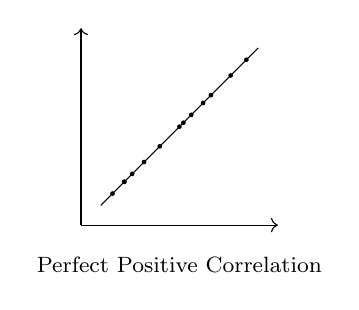
\begin{tikzpicture}[scale=0.5]
      \draw[->] (0, 0) -- (5, 0);
      \draw[->] (0, 0) -- (0, 5);
      \draw (0.5, 0.5) -- (4.5, 4.5);
      \fill (0.8, 0.8) circle (0.06);
      \fill (1.1, 1.1) circle (0.06);
      \fill (1.1, 1.1) circle (0.06);
      \fill (1.3, 1.3) circle (0.06);
      \fill (1.6, 1.6) circle (0.06);
      \fill (2.0, 2.0) circle (0.06);
      \fill (2.5, 2.5) circle (0.06);
      \fill (2.6, 2.6) circle (0.06);
      \fill (2.8, 2.8) circle (0.06);
      \fill (3.1, 3.1) circle (0.06);
      \fill (3.3, 3.3) circle (0.06);
      \fill (3.8, 3.8) circle (0.06);
      \fill (4.2, 4.2) circle (0.06);
      \node at (2.5, -1) {\footnotesize{Perfect Positive Correlation}};
    \end{tikzpicture}
    \hspace{1cm}
    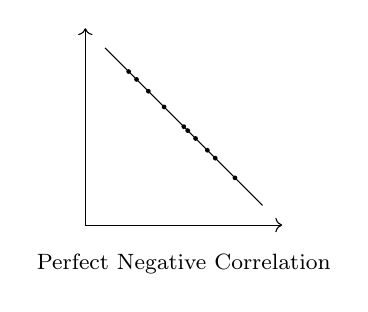
\begin{tikzpicture}[scale=0.5]
      \draw[->] (0, 0) -- (5, 0);
      \draw[->] (0, 0) -- (0, 5);
      \draw (0.5, 4.5) -- (4.5, 0.5);
      \fill (1.1, 3.9) circle (0.06);
      \fill (1.3, 3.7) circle (0.06);
      \fill (1.6, 3.4) circle (0.06);
      \fill (2.0, 3.0) circle (0.06);
      \fill (2.5, 2.5) circle (0.06);
      \fill (2.6, 2.4) circle (0.06);
      \fill (2.8, 2.2) circle (0.06);
      \fill (3.1, 1.9) circle (0.06);
      \fill (3.3, 1.7) circle (0.06);
      \fill (3.8, 1.2) circle (0.06);
      \node at (2.5, -1) {\footnotesize{Perfect Negative Correlation}};
    \end{tikzpicture}
  \end{center}
  \begin{center}
    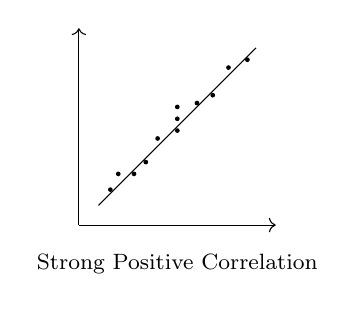
\begin{tikzpicture}[scale=0.5]
      \draw[->] (0, 0) -- (5, 0);
      \draw[->] (0, 0) -- (0, 5);
      \draw (0.5, 0.5) -- (4.5, 4.5);
      \fill (0.8, 0.9) circle (0.06);
      \fill (1.0, 1.3) circle (0.06);
      \fill (1.4, 1.3) circle (0.06);
      \fill (1.7, 1.6) circle (0.06);
      \fill (2.0, 2.2) circle (0.06);
      \fill (2.5, 2.4) circle (0.06);
      \fill (2.5, 2.7) circle (0.06);
      \fill (2.5, 3.0) circle (0.06);
      \fill (3.0, 3.1) circle (0.06);
      \fill (3.4, 3.3) circle (0.06);
      \fill (3.8, 4.0) circle (0.06);
      \fill (4.28, 4.2) circle (0.06);
      \node at (2.5, -1) {\footnotesize{Strong Positive Correlation}};
    \end{tikzpicture}
    \hspace{1cm}
    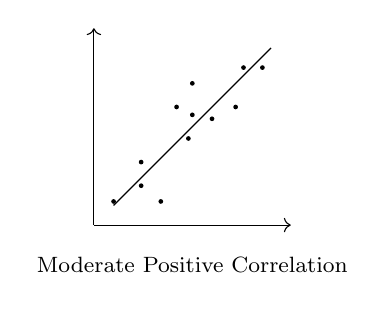
\begin{tikzpicture}[scale=0.5]
      \draw[->] (0, 0) -- (5, 0);
      \draw[->] (0, 0) -- (0, 5);
      \draw (0.5, 0.5) -- (4.5, 4.5);
      \fill (0.5, 0.6) circle (0.06);
      \fill (1.2, 1.6) circle (0.06);
      \fill (1.7, 0.6) circle (0.06);
      \fill (1.2, 1.0) circle (0.06);
      \fill (2.4, 2.2) circle (0.06);
      \fill (2.5, 2.8) circle (0.06);
      \fill (2.5, 3.6) circle (0.06);
      \fill (2.1, 3.0) circle (0.06);
      \fill (3.0, 2.7) circle (0.06);
      \fill (3.6, 3.0) circle (0.06);
      \fill (3.8, 4.0) circle (0.06);
      \fill (4.28, 4.0) circle (0.06);
      \node at (2.5, -1) {\footnotesize{Moderate Positive Correlation}};
    \end{tikzpicture}
  \end{center}
  \begin{center}
    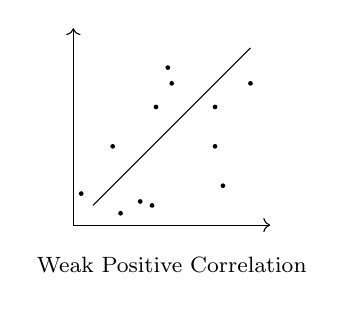
\begin{tikzpicture}[scale=0.5]
      \draw[->] (0, 0) -- (5, 0);
      \draw[->] (0, 0) -- (0, 5);
      \draw (0.5, 0.5) -- (4.5, 4.5);
      \fill (0.2, 0.8) circle (0.06);
      \fill (1.0, 2.0) circle (0.06);
      \fill (1.7, 0.6) circle (0.06);
      \fill (1.2, 0.3) circle (0.06);
      \fill (2.4, 4.0) circle (0.06);
      \fill (2.5, 3.6) circle (0.06);
      \fill (2.0, 0.5) circle (0.06);
      \fill (2.1, 3.0) circle (0.06);
      \fill (3.6, 2.0) circle (0.06);
      \fill (3.6, 3.0) circle (0.06);
      \fill (3.8, 1.0) circle (0.06);
      \fill (4.5, 3.6) circle (0.06);
      \node at (2.5, -1) {\footnotesize{Weak Positive Correlation}};
    \end{tikzpicture}
    \hspace{1cm}
    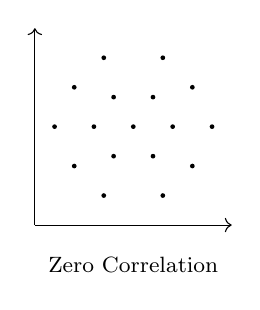
\begin{tikzpicture}[scale=0.5]
      \draw[->] (0, 0) -- (5, 0);
      \draw[->] (0, 0) -- (0, 5);
      \fill (1.75, 4.25) circle (0.06);
      \fill (3.25, 4.25) circle (0.06);
      \fill (1.0, 3.5) circle (0.06);
      \fill (4.0, 3.5) circle (0.06);
      \fill (2, 3.25) circle (0.06);
      \fill (3, 3.25) circle (0.06);
      \fill (0.5, 2.5) circle (0.06);
      \fill (1.5, 2.5) circle (0.06);
      \fill (2.5, 2.5) circle (0.06);
      \fill (3.5, 2.5) circle (0.06);
      \fill (4.5, 2.5) circle (0.06);
      \fill (1.0, 1.5) circle (0.06);
      \fill (4.0, 1.5) circle (0.06);
      \fill (2.0, 1.75) circle (0.06);
      \fill (3.0, 1.75) circle (0.06);
      \fill (1.75, 0.75) circle (0.06);
      \fill (3.25, 0.75) circle (0.06);
      \node at (2.5, -1) {\footnotesize{Zero Correlation}};
    \end{tikzpicture}
  \end{center}

  \begin{enumerate}
    \item If every single point in the scatter plot is on the line of best fit, then it's
          a perfect positive correlation. If the slope of the line of best fit is
          positive, then it's a positive correlation. If the slope of the line of best
          fit is negative, then it's a negative correlation.

    \item If the points in the scatter plot are scattered around the line of best fit
          with non-zero slope, then the closer the points are to the line of best fit,
          the stronger the correlation is.

    \item If the points in the scatter plot are scattered evenly around the whole plot
          with no obvious pattern, then there is no correlation between the two
          variables, aka zero correlation.
  \end{enumerate}

  \subsection*{Correlation Coefficient}

  Telling the correlation between two variables by looking at the scatter plot is
  not a very accurate way. To accurately measure the correlation between two sets
  of data, we need to use a coefficient that can distinguish the strength of the
  correlation.

  \begin{center}
    \begin{tikzpicture}
      \draw[->] (0, 0) -- (5, 0);
      \draw[->] (0, 0) -- (0, 5);
      \draw[dashed] (2.2, 0.0) -- (2.2, 5.0);
      \draw[dashed] (0.0, 2.2) -- (5.0, 2.2);
      \fill (0.2, 0.8) circle (0.06);
      \fill (1.0, 2.0) circle (0.06);
      \fill (1.7, 0.6) circle (0.06);
      \fill (1.2, 0.3) circle (0.06);
      \fill (2.4, 4.0) circle (0.06);
      \fill (2.5, 3.6) circle (0.06);
      \fill (2.0, 0.5) circle (0.06);
      \fill (2.1, 3.0) circle (0.06);
      \fill (3.6, 2.0) circle (0.06);
      \fill (3.6, 3.0) circle (0.06);
      \fill (3.8, 1.0) circle (0.06);
      \fill (4.5, 3.6) circle (0.06);
    \end{tikzpicture}
  \end{center}

  Let the mean value of two sets of data be $x_1, x_2, \dots, x_n$ and $y_1, y_2,
    \dots, y_n$ be $\bar{x}$ and $\bar{y}$ respectively. Draw two lines $x =
    \bar{x}$ and $y = \bar{y}$ on the scatter plot of the two sets of data,
  splitting the plot into four quadrants, as shown in the figure above. Now the
  origin of the plot is at $(\bar{x}, \bar{y})$. If a point $(x_i, y_i)$ is in
  the first or the third quadrant, then $(x_i - \bar{x})(y_i - \bar{y})$ is
  positive. As discussed in the previous section, if the correlation is positive,
  the points are scattering around the line of best fit with positive slope.
  Therefore, the points are more likely to be in the first or the third quadrant.
  That means, there are more positive value of $(x_i - \bar{x})(y_i - \bar{y})$
  than negative value, therefore the value of $\sum{(x_i - \bar{x})(y_i -
      \bar{y})}$ is positive. The higher the correlation is, the more points are in
  the first or the third quadrant, the higher the positive value of $\sum{(x_i -
      \bar{x})(y_i - \bar{y})}$ is.

  On the other hand, if a point $(x_i, y_i)$ is in the second or the fourth
  quadrant, then $(x_i - \bar{x})(y_i - \bar{y})$ is negative, which means there
  are more negative value of $(x_i - \bar{x})(y_i - \bar{y})$ than positive
  value, therefore the value of $\sum{(x_i - \bar{x})(y_i - \bar{y})}$ is
  negative. Similarly, he higher the correlation is, the lower the negative value
  of $\sum{(x_i - \bar{x})(y_i - \bar{y})}$ is.

  Hence, the value and the sign of $\sum{(x_i - \bar{x})(y_i - \bar{y})}$ can be
  used to measure the correlation between two sets of data. The value of
  $\sum{(x_i - \bar{x})(y_i - \bar{y})}$ will be affected by the measurement unit
  of the data. To make the value of $\sum{(x_i - \bar{x})(y_i - \bar{y})}$
  independent of the measurement unit, we define the correlation coefficient of
  two sets of data $x_1, x_2, \dots, x_n$ and $y_1, y_2, \dots, y_n$ as:

  \begin{cequation}
    r = \frac{\sum{(x_i - \bar{x})(y_i - \bar{y})}}{\sqrt{\sum{(x_i - \bar{x})^2}\sum{(y_i - \bar{y})^2}}}
  \end{cequation}

  The value of $r$ is always between $-1$ and $1$. If $r = 0$, then there is no
  correlation between the two sets of data. If $r > 0$, then the correlation is
  positive. If $r < 0$, then the correlation is negative. The absolute value of
  $r$ is the strength of the correlation, and is generally divided as follows:

  \begin{enumerate}
    \item $|r| = 1$: perfect correlation
    \item $0 < |r| < 0.3$: weak correlation
    \item $0.3 \leq |r| < 0.7$: moderate correlation
    \item $0.7 \leq |r| \leq 1$: strong correlation
  \end{enumerate}

  Dividing both the denominator and the numerator of the formula of $r$ by the
  number of data points $n$, then the numerator is the mean value of $(x_i -
    \bar{x})(y_i - \bar{y})$, and the denominator is the product of the standard
  deviation of $x_1, x_2, \dots, x_n$ and $y_1, y_2, \dots, y_n$. Similar to the
  standard deviation, there is an easier way to calculate the correlation
  coefficient:

  \begin{flalign*}
    r & = \frac{\sum{(x_i - \bar{x})(y_i - \bar{y})}}{\sqrt{\sum{(x_i - \bar{x})^2}\sum{(y_i - \bar{y})^2}}}                                                                                                                                                                                                                   & \\
      & = \frac{\sum{(x_iy_i - x_i\bar{y} - \bar{x}y_i + \bar{x}\bar{y})}}{\sqrt{\sum{(x_i^2 - 2x_i\bar{x} + \bar{x}^2)\sum{(y_i^2 - 2y_i\bar{y} + \bar{y}^2)}}}}                                                                                                                                                                \\
      & = \frac{\sum{x_iy_i} -\bar{y}\sum{x_i} - y_i\sum{\bar{x}} + \sum\bar{x}\bar{y}}{\sqrt{\sum{(x_i^2 - 2x_i\bar{x} + \bar{x}^2)\sum{(y_i^2 - 2y_i\bar{y} + \bar{y}^2)}}}}                                                                                                                                                   \\
      & = \frac{\frac{\sum{x_iy_i} -\bar{y}\sum{x_i} - y_i\sum{\bar{x}} + \sum\bar{x}\bar{y}}{n}}{\frac{\sqrt{\sum{(x_i^2 - 2x_i\bar{x} + \bar{x}^2)\sum{(y_i^2 - 2y_i\bar{y} + \bar{y}^2)}}}}{n}}                                                                                                                               \\
      & = \frac{\frac{\sum{x_iy_i}}{n} - \frac{\bar{y}\sum{x_i}}{n} - \frac{y_i\sum{\bar{x}}}{n} + \frac{\sum\bar{x}\bar{y}}{n}}{\sqrt{\frac{\sum{(x_i^2 - 2x_i\bar{x} + \bar{x}^2)\sum{(y_i^2 - 2y_i\bar{y} + \bar{y}^2)}}}{n \cdot n}}}                                                                                        \\
      & = \frac{\frac{\sum{x_iy_i}}{n} - \frac{\bar{y}\sum{x_i}}{n} - \frac{\bar{x}\sum{y_i}}{n} + \frac{n\bar{x}\bar{y}}{n}}{\sqrt{\left(\frac{\sum{x_i^2}}{n} - \frac{2\bar{x}\sum{x_i}}{n} + \frac{\sum{\bar{x}^2}}{n}\right)\left(\frac{\sum{y_i^2}}{n} - \frac{2\bar{y}\sum{y_i}}{n} + \frac{\sum{\bar{y}^2}}{n}\right)}}   \\
      & = \frac{\frac{\sum{x_iy_i}}{n} - \bar{x}\bar{y} - \bar{x}\bar{y} + \bar{x}\bar{y}}{\sqrt{\left(\frac{\sum{x_i^2}}{n} - 2\bar{x}^2 + \frac{n\bar{x}^2}{n}\right)\left(\frac{\sum{y_i^2}}{n} - 2\bar{y}^2 + \frac{n\bar{y}^2}{n}\right)}}                                                                                  \\
      & = \frac{\frac{\sum{x_iy_i}}{n} - \bar{x}\bar{y}}{\sqrt{\left(\frac{\sum{x_i^2}}{n} - 2\bar{x}^2 + \bar{x}^2\right)\left(\frac{\sum{y_i^2}}{n} - 2\bar{y}^2 + \bar{y}^2\right)}}                                                                                                                                          \\
      & = \frac{\frac{\sum{x_iy_i}}{n} - \bar{x}\bar{y}}{\sqrt{\left(\frac{\sum{x_i^2}}{n} - \bar{x}^2\right)\left(\frac{\sum{y_i^2}}{n} - \bar{y}^2\right)}}                                                                                                                                                                    \\
  \end{flalign*}

  \subsection{Practice 10}

  \begin{enumerate}
    \item The table below shows the height (in $cm$) and weight (in $kg$) of 15
          10-year-old children:
          \begin{center}
            \begin{tabular}{|c|c|}
              \hline
              Height & Weight \\
              \hline
              126    & 41     \\
              130    & 42     \\
              110    & 38     \\
              123    & 36     \\
              118    & 33     \\
              130    & 45     \\
              127    & 34     \\
              124    & 35     \\
              116    & 30     \\
              112    & 32     \\
              113    & 31     \\
              121    & 40     \\
              115    & 34     \\
              120    & 35     \\
              118    & 33     \\
              \hline
            \end{tabular}
          \end{center}
          Calculate the correlation coefficient of the height and the weight of the 15 children, and determine on the strength of the correlation.
          \sol{}
          \begin{center}
            \resizebox{\columnwidth-4.6em}{!}{
              \begin{tabular}{|c|c|c|c|c|}
                \hline
                $x_i$       & $y_i$       & $x_i^2$       & $y_i^2$       & $x_iy_i$       \\
                \hline
                126         & 41          & 15876         & 1681          & 5166           \\
                130         & 42          & 16900         & 1764          & 5460           \\
                110         & 38          & 12100         & 1444          & 4180           \\
                123         & 36          & 15129         & 1296          & 4428           \\
                118         & 33          & 13924         & 1089          & 3894           \\
                130         & 45          & 16900         & 2025          & 5850           \\
                127         & 34          & 16129         & 1156          & 4318           \\
                124         & 35          & 15376         & 1225          & 4340           \\
                116         & 30          & 13456         & 900           & 3480           \\
                112         & 32          & 12544         & 1024          & 3584           \\
                113         & 31          & 12769         & 961           & 3503           \\
                121         & 40          & 14641         & 1600          & 4840           \\
                115         & 34          & 13225         & 1156          & 3910           \\
                120         & 35          & 14400         & 1225          & 4200           \\
                118         & 33          & 13924         & 1089          & 3894           \\
                \hline
                \hline
                $\sum{x_i}$ & $\sum{y_i}$ & $\sum{x_i^2}$ & $\sum{y_i^2}$ & $\sum{x_iy_i}$ \\
                \hline
                1803        & 539         & 217293        & 19635         & 65047          \\
                \hline
              \end{tabular}
            }
          \end{center}
          \begin{flalign*}
            \bar{x} & = \frac{1803}{15} = 120.2                                                                                                             \\
            \bar{y} & = \frac{539}{15} = 35.93                                                                                                              \\
            r       & = \frac{\frac{65047}{15} - 120.2 \cdot 35.93}{\sqrt{\left(\frac{217293}{15} - 120.2^2\right)\left(\frac{19635}{15} - 35.93^2\right)}} \\
                    & = 0.6631
          \end{flalign*}
          According to the result of the calculation, the height and the weight of the 15 children are positively and moderetely correlated.

    \item In order to study the relationship between the systolic blood pressure (in
          $\mathit{mmHg}$) and the age (in $year$) of human, a medical school collected
          the data of 13 male patients:
          \begin{center}
            \begin{tabular}{|c|c|}
              \hline
              Age & Systolic Blood Pressure \\
              \hline
              51  & 130                     \\
              22  & 141                     \\
              23  & 124                     \\
              31  & 126                     \\
              33  & 117                     \\
              49  & 135                     \\
              58  & 143                     \\
              53  & 138                     \\
              44  & 132                     \\
              55  & 143                     \\
              42  & 133                     \\
              45  & 115                     \\
              25  & 147                     \\
              \hline
            \end{tabular}
          \end{center}
          \begin{enumerate}
            \item Construct a scatter diagram of the data. \sol{}
                  \begin{center}
                    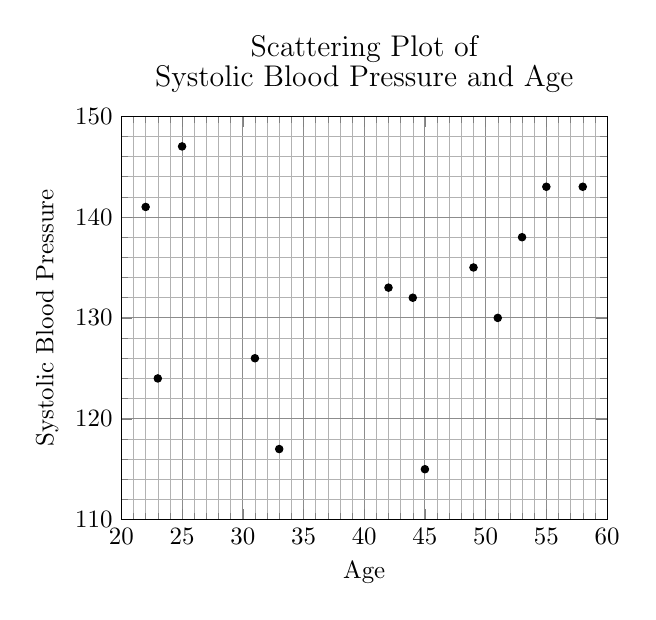
\begin{tikzpicture}[scale=0.9]
                      \begin{axis}[
                          title style = {align = center},
                          title={\large{Scattering Plot of} \\ \large{Systolic Blood Pressure and Age}},
                          xlabel={Age},
                          ylabel={Systolic Blood Pressure},
                          xmin=20, xmax=60,
                          ymin=110, ymax=150,
                          xtick={20, 25, ..., 60},
                          ytick={110, 120, 130, 140, 150},
                          grid=both,
                          grid style={line width=.2pt, draw=gray!60},
                          major grid style={line width=.4pt,draw=gray!90},
                          minor tick num=4,
                        ]
                        \addplot[mark=*, mark size=1.5, mark options={solid, fill=black}, only marks] coordinates {(51, 130) (22, 141) (23, 124) (31, 126) (33, 117) (49, 135) (58, 143) (53, 138) (44, 132) (55, 143) (42, 133) (45, 115) (25, 147)};
                      \end{axis}
                    \end{tikzpicture}
                  \end{center}
            \item Calculate the correlation coefficient of the age and the systolic blood
                  pressure of the 13 patients, and determine on the strength of the correlation.
                  \sol{}
                  \begin{center}
                    \resizebox{\columnwidth-4.6em}{!}{
                      \begin{tabular}{|c|c|c|c|c|}
                        \hline
                        $x_i$       & $y_i$       & $x_i^2$       & $y_i^2$       & $x_iy_i$       \\
                        \hline
                        51          & 130         & 2601          & 16900         & 6630           \\
                        22          & 141         & 484           & 19881         & 3102           \\
                        23          & 124         & 529           & 15376         & 2852           \\
                        31          & 126         & 961           & 15876         & 3906           \\
                        33          & 117         & 1089          & 13689         & 3861           \\
                        49          & 135         & 2401          & 18225         & 6615           \\
                        58          & 143         & 3364          & 20449         & 8294           \\
                        53          & 138         & 2809          & 19044         & 7314           \\
                        44          & 132         & 1936          & 17424         & 5808           \\
                        55          & 143         & 3025          & 20449         & 7865           \\
                        42          & 133         & 1764          & 17689         & 5586           \\
                        45          & 155         & 2025          & 24025         & 6975           \\
                        25          & 147         & 625           & 21609         & 3675           \\
                        \hline
                        \hline
                        $\sum{x_i}$ & $\sum{y_i}$ & $\sum{x_i^2}$ & $\sum{y_i^2}$ & $\sum{x_iy_i}$ \\
                        \hline
                        531         & 1764        & 23613         & 240636        & 72483          \\
                        \hline
                      \end{tabular}
                    }
                  \end{center}
                  \begin{flalign*}
                    \bar{x} & = \frac{531}{13} = 40.85                                                                                                                & \\
                    \bar{y} & = \frac{1764}{13} = 135.69                                                                                                                \\
                    r       & = \frac{\frac{72483}{13} - 40.85 \cdot 135.69}{\sqrt{\left(\frac{23613}{13} - 40.85^2\right)\left(\frac{240636}{13} - 135.69^2\right)}}   \\
                            & = 0.2748
                  \end{flalign*}
                  According to the result of the calculation, the height and the weight of the 15 children are positively and weakly correlated.
          \end{enumerate}
  \end{enumerate}

  \subsection{Exercise 18.6}

  \begin{enumerate}
    \item The table below shows the value of fixed assets and total assets (in 10
          thousand dollar) of 10 enterprises of the same industry:
          \begin{center}
            \begin{tabular}{|c|c|c|}
              \hline
              No. of Enterprise & Fixed Assets & Total Assets \\
              \hline
              1                 & 200          & 638          \\
              2                 & 314          & 605          \\
              3                 & 318          & 524          \\
              4                 & 409          & 815          \\
              5                 & 415          & 913          \\
              6                 & 502          & 928          \\
              7                 & 910          & 1019         \\
              8                 & 1022         & 1219         \\
              9                 & 1210         & 1516         \\
              10                & 1225         & 1624         \\
              \hline
            \end{tabular}
          \end{center}
          \begin{enumerate}
            \item Construct a scatter diagram of the data. \sol{}
                  \begin{center}
                    \resizebox{\columnwidth-4.6em}{!}{
                      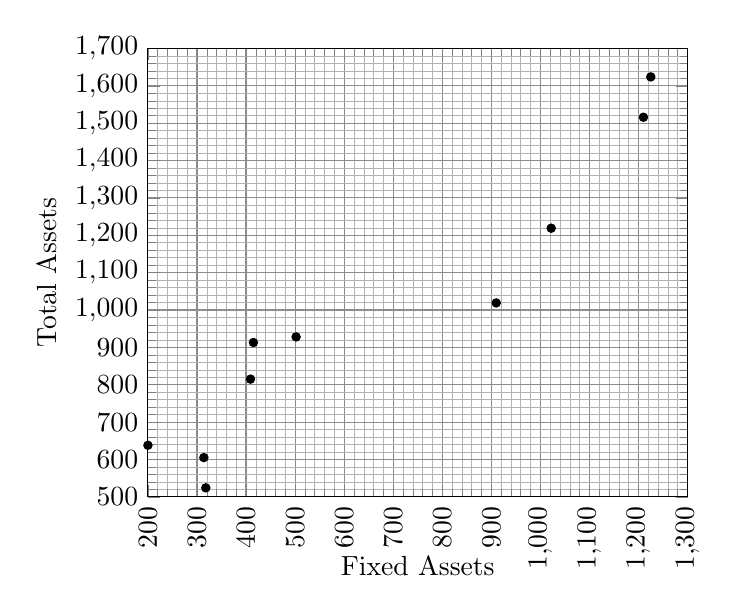
\begin{tikzpicture}
                        \begin{axis}[
                            xlabel={Fixed Assets},
                            ylabel={Total Assets},
                            xmin=200, xmax=1300,
                            ymin=500, ymax=1700,
                            xtick={200, 300, ..., 1300},
                            ytick={500, 600, ..., 1700},
                            grid=both,
                            grid style={line width=.2pt, draw=gray!60},
                            major grid style={line width=.4pt,draw=gray!90},
                            minor tick num=4,
                            xticklabel style={rotate=90},
                            x label style={at={(axis description cs:0.5,-0.11)},anchor=north},
                          ]
                          \addplot[mark=*, mark size=1.5, mark options={solid, fill=black}, only marks] coordinates {(200, 638) (314, 605) (318, 524) (409, 815) (415, 913) (502, 928) (910, 1019) (1022, 1219) (1210, 1516) (1225, 1624)};
                        \end{axis}
                      \end{tikzpicture}
                    }
                  \end{center}

            \item Calculate the mean value of fixed assets and total assets respectively. \sol{}
                  \begin{flalign*}
                    \text{Mean of fixed assets } \bar{x} & = \frac{200 + 314 + \cdots + 1225}{10} & \\
                                                         & = \frac{6525}{10}                        \\
                                                         & = 652.5                                  \\
                                                         & = \$652,500,000                          \\
                    \\
                    \text{Mean of total assets } \bar{y} & = \frac{638 + 605 + \cdots + 1624}{10}   \\
                                                         & = \frac{9801}{10}                        \\
                                                         & = 980.1                                  \\
                                                         & = \$980,100,000
                  \end{flalign*}

            \item Find the correlation coefficient of the fixed assets and the total assets, and
                  determine on the strength of the correlation. \sol{}
                  \begin{center}
                    \resizebox{\columnwidth-4.6em}{!}{
                      \begin{tabular}{|c|c|c|c|c|}
                        \hline
                        $x_i$       & $y_i$       & $x_i^2$       & $y_i^2$       & $x_iy_i$       \\
                        \hline
                        200         & 638         & 40000         & 407044        & 127600         \\
                        314         & 605         & 98596         & 366025        & 189970         \\
                        318         & 524         & 101124        & 274576        & 166632         \\
                        409         & 815         & 167281        & 664225        & 333335         \\
                        415         & 913         & 172225        & 833569        & 378895         \\
                        502         & 928         & 252004        & 861184        & 465856         \\
                        910         & 1019        & 828100        & 1038361       & 927290         \\
                        1022        & 1219        & 1044484       & 1485961       & 1245818        \\
                        1210        & 1516        & 1464100       & 2298256       & 1834360        \\
                        1225        & 1624        & 1500625       & 2637376       & 1989400        \\
                        \hline
                        \hline
                        $\sum{x_i}$ & $\sum{y_i}$ & $\sum{x_i^2}$ & $\sum{y_i^2}$ & $\sum{x_iy_i}$ \\
                        \hline
                        6525        & 9801        & 5668539       & 10866577      & 7659156        \\
                        \hline
                      \end{tabular}
                    }
                  \end{center}
                  \begin{flalign*}
                    r & = \frac{\frac{7659156}{13} - 652.5 \cdot 980.1}{\sqrt{\left(\frac{5668539}{13} - 652.5^2\right)\left(\frac{10866577}{13} - 980.1^2\right)}} & \\
                      & = 0.9478
                  \end{flalign*}
                  According to the result of the calculation, According to the result of the calculation, the value of fixed assets and total assets of theese 10 enterprises are positively and strongly correlated.
          \end{enumerate}

    \item The table shows the marks of Mathematics and Ecomoics of 15 students:
          \begin{center}
            \begin{tabular}{|c|c|}
              \hline
              Mathematics & Economics \\
              \hline
              83          & 79        \\
              50          & 61        \\
              62          & 70        \\
              90          & 86        \\
              68          & 69        \\
              61          & 68        \\
              58          & 62        \\
              62          & 80        \\
              71          & 70        \\
              63          & 74        \\
              72          & 77        \\
              54          & 54        \\
              64          & 77        \\
              48          & 50        \\
              81          & 92        \\
              \hline
            \end{tabular}
          \end{center}
          \begin{enumerate}
            \item Construct a scatter diagram of the data. \sol{}
                  \begin{center}
                    \resizebox{\columnwidth-4.6em}{!}{
                      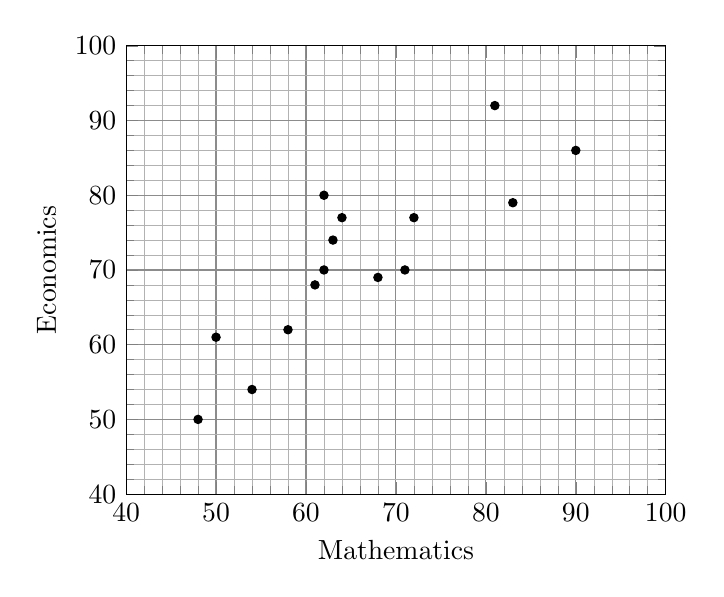
\begin{tikzpicture}
                        \begin{axis}[
                            xlabel={Mathematics},
                            ylabel={Economics},
                            xmin=40, xmax=100,
                            ymin=40, ymax=100,
                            xtick={40, 50, ..., 100},
                            ytick={40, 50, ..., 100},
                            grid=both,
                            grid style={line width=.2pt, draw=gray!60},
                            major grid style={line width=.4pt,draw=gray!90},
                            minor tick num=4,
                          ]
                          \addplot[mark=*, mark size=1.5, mark options={solid, fill=black}, only marks] coordinates {(83, 79) (50, 61) (62, 70) (90, 86) (68, 69) (61, 68) (58, 62) (62, 80) (71, 70) (63, 74) (72, 77) (54, 54) (64, 77) (48, 50) (81, 92)};
                        \end{axis}
                      \end{tikzpicture}
                    }
                  \end{center}

            \item Find the correlation coefficient of the marks of Mathematics and the Economics,
                  and determine on the strength of the correlation. \sol{}
                  \begin{center}
                    \resizebox{\columnwidth-4.6em}{!}{
                      \begin{tabular}{|c|c|c|c|c|}
                        \hline
                        $x_i$       & $y_i$       & $x_i^2$       & $y_i^2$       & $x_iy_i$       \\
                        \hline
                        83          & 79          & 6889          & 6241          & 6557           \\
                        50          & 61          & 2500          & 3721          & 3050           \\
                        62          & 70          & 3844          & 4900          & 4340           \\
                        90          & 86          & 8100          & 7396          & 7740           \\
                        68          & 69          & 4624          & 4761          & 4692           \\
                        61          & 68          & 3721          & 4624          & 4148           \\
                        58          & 62          & 3364          & 3844          & 3596           \\
                        62          & 80          & 3844          & 6400          & 4960           \\
                        71          & 70          & 5041          & 4900          & 4970           \\
                        63          & 74          & 3969          & 5476          & 4662           \\
                        72          & 77          & 5184          & 5929          & 5544           \\
                        54          & 54          & 2916          & 2916          & 2916           \\
                        64          & 77          & 4096          & 5929          & 4928           \\
                        48          & 50          & 2304          & 2500          & 2400           \\
                        81          & 92          & 6561          & 8464          & 7452           \\
                        \hline
                        \hline
                        $\sum{x_i}$ & $\sum{y_i}$ & $\sum{x_i^2}$ & $\sum{y_i^2}$ & $\sum{x_iy_i}$ \\
                        \hline
                        987         & 1069        & 66957         & 78001         & 71955          \\
                        \hline
                      \end{tabular}
                    }
                  \end{center}
                  \begin{flalign*}
                    \bar{x} & = \frac{987}{15} = 65.8                                                                                                              \\
                    \bar{y} & = \frac{1069}{15} = 71.27                                                                                                            \\
                    r       & = \frac{\frac{71955}{15} - 65.8 \cdot 71.27}{\sqrt{\left(\frac{66957}{15} - 65.8^2\right)\left(\frac{78001}{15} - 71.27^2\right)}} & \\
                            & = 0.8445
                  \end{flalign*}
                  According to the result of the calculation, the marks of Mathematics and the Economics are positively and strongly correlated.

          \end{enumerate}

    \item The table below shows the marks of 16 students in the Chinese language minor
          test. The paper was split into two sections: Vernacular and Classical Chinese
          and their full marks were 60 and 40 respectively.
          \begin{center}
            \begin{tabular}{|c|c|}
              \hline
              Vernacular Chinese & Classical Chinese \\
              \hline
              43                 & 30                \\
              50                 & 21                \\
              38                 & 20                \\
              45                 & 19                \\
              58                 & 15                \\
              47                 & 18                \\
              32                 & 30                \\
              36                 & 28                \\
              38                 & 26                \\
              51                 & 30                \\
              44                 & 29                \\
              28                 & 29                \\
              49                 & 22                \\
              42                 & 32                \\
              46                 & 33                \\
              35                 & 25                \\
              \hline
            \end{tabular}
          \end{center}
          \begin{enumerate}
            \item Construct a scatter diagram of the data. \sol{}
                  \begin{center}
                    \resizebox{\columnwidth-4.6em}{!}{
                      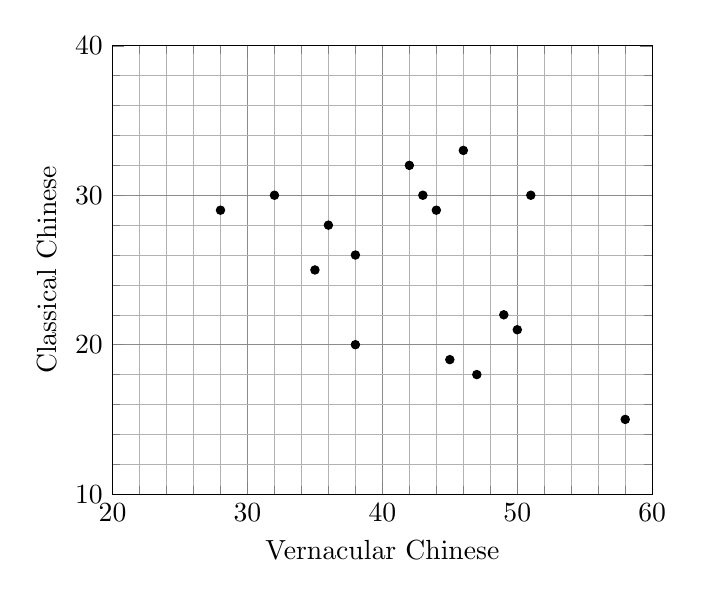
\begin{tikzpicture}
                        \begin{axis}[
                            xlabel=Vernacular Chinese,
                            ylabel=Classical Chinese,
                            xmin=20, xmax=60,
                            ymin=10, ymax=40,
                            xtick={20, 30, ..., 60},
                            ytick={10, 20, ..., 40},
                            grid=both,
                            grid style={line width=.2pt, draw=gray!60},
                            major grid style={line width=.4pt,draw=gray!90},
                            minor tick num=4,
                          ]
                          \addplot[mark=*, mark size=1.5, mark options={solid, fill=black}, only marks] coordinates {(43, 30) (50, 21) (38, 20) (45, 19) (58, 15) (47, 18) (32, 30) (36, 28) (38, 26) (51, 30) (44, 29) (28, 29) (49, 22) (42, 32) (46, 33) (35, 25)};
                        \end{axis}
                      \end{tikzpicture}
                    }
                  \end{center}

            \item Find the correlation coefficient of the marks of Vernacular Chinese and the
                  Classical Chinese, and determine on the strength of the correlation. \sol{}
                  \begin{center}
                    \resizebox{\columnwidth-4.6em}{!}{
                      \begin{tabular}{|c|c|c|c|c|}
                        \hline
                        $x_i$       & $y_i$       & $x_i^2$       & $y_i^2$       & $x_iy_i$       \\
                        \hline
                        43          & 30          & 1849          & 900           & 1290           \\
                        50          & 21          & 2500          & 441           & 1050           \\
                        38          & 20          & 1444          & 400           & 760            \\
                        45          & 19          & 2025          & 361           & 855            \\
                        58          & 15          & 3364          & 225           & 870            \\
                        47          & 18          & 2209          & 324           & 846            \\
                        32          & 30          & 1024          & 900           & 960            \\
                        36          & 28          & 1296          & 784           & 1008           \\
                        38          & 26          & 1444          & 676           & 988            \\
                        51          & 30          & 2601          & 900           & 1530           \\
                        44          & 29          & 1936          & 841           & 1276           \\
                        28          & 29          & 784           & 841           & 812            \\
                        49          & 22          & 2401          & 484           & 1078           \\
                        42          & 32          & 1764          & 1024          & 1344           \\
                        46          & 33          & 2116          & 1089          & 1518           \\
                        35          & 25          & 1225          & 625           & 875            \\
                        \hline
                        \hline
                        $\sum{x_i}$ & $\sum{y_i}$ & $\sum{x_i^2}$ & $\sum{y_i^2}$ & $\sum{x_iy_i}$ \\
                        \hline
                        682         & 407         & 29982         & 10815         & 17060          \\
                        \hline
                      \end{tabular}
                    }
                  \end{center}
                  \begin{flalign*}
                    \bar{x} & = \frac{682}{16} = 42.62                                                                                                               \\
                    \bar{y} & = \frac{407}{16} = 25.44                                                                                                               \\
                    r       & = \frac{\frac{17060}{16} - 42.62 \cdot 25.44}{\sqrt{\left(\frac{29982}{16} - 42.62^2\right)\left(\frac{10815}{16} - 25.44^2\right)}} & \\
                            & = -0.4444
                  \end{flalign*}
                  According to the result of the calculation, the marks of Vernacular Chinese and Classical Chinese are negatively and moderately correlated.
          \end{enumerate}

    \item Below shows the the service costs and values of properties sold by a property
          broker in 5 trades:
          \begin{center}
            \begin{tabular}{|c|c|}
              \hline
              Service Costs (in \$100) & Value of Prop. (in \$10k) \\
              \hline
              16.5                     & 3.9                       \\
              17.4                     & 4.2                       \\
              16.8                     & 4.1                       \\
              17.9                     & 4.5                       \\
              18.4                     & 4.8                       \\
              \hline
            \end{tabular}
          \end{center}
          Find the correlation coefficient of the service costs and the values of properties in these 5 trades, and determine on the strength of the correlation.
          \sol{}
          \begin{center}
            \resizebox{\columnwidth-4.6em}{!}{
              \begin{tabular}{|c|c|c|c|c|}
                \hline
                $x_i$       & $y_i$       & $x_i^2$       & $y_i^2$       & $x_iy_i$       \\
                \hline
                16.5        & 3.9         & 272.25        & 15.21         & 64.35          \\
                17.4        & 4.2         & 302.76        & 17.64         & 73.08          \\
                16.8        & 4.1         & 282.24        & 16.81         & 68.88          \\
                17.9        & 4.5         & 320.41        & 20.25         & 80.55          \\
                18.4        & 4.8         & 338.56        & 23.04         & 88.32          \\
                \hline
                \hline
                $\sum{x_i}$ & $\sum{y_i}$ & $\sum{x_i^2}$ & $\sum{y_i^2}$ & $\sum{x_iy_i}$ \\
                \hline
                87.0        & 21.5        & 1516.22       & 92.95         & 375.18         \\
                \hline
              \end{tabular}
            }
          \end{center}
          \begin{flalign*}
            \bar{x} & = \frac{87.0}{5} = 17.4                                                                                                          \\
            \bar{y} & = \frac{21.5}{5} = 4.3                                                                                                           \\
            r       & = \frac{\frac{375.18}{5} - 17.4 \cdot 4.3}{\sqrt{\left(\frac{1516.22}{5} - 17.4^2\right)\left(\frac{92.95}{5} - 4.3^2\right)}} & \\
                    & = 0.9818
          \end{flalign*}
          According to the result of the calculation, the service costs and the values of properties are positively and strongly correlated.

    \item The table below shows the degree of labor mechanization and labor productivity:
          \begin{center}
            \begin{tabular}{|c|c|}
              \hline
              Mechanization Degree (\%) & Productivity (\$/pax) \\
              \hline
              40                        & 800                   \\
              45                        & 880                   \\
              50                        & 1010                  \\
              55                        & 1034                  \\
              60                        & 980                   \\
              65                        & 1030                  \\
              70                        & 1077                  \\
              75                        & 1344                  \\
              80                        & 1460                  \\
              \hline
            \end{tabular}
          \end{center}
          \begin{enumerate}
            \item Construct a scatter diagram of the data. \sol{}
                  \begin{center}
                    \resizebox{\columnwidth-4.6em}{!}{
                      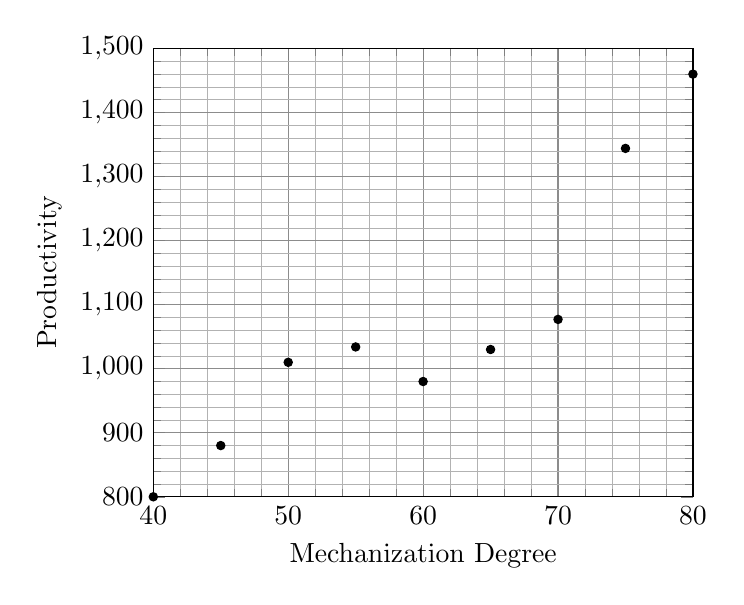
\begin{tikzpicture}
                        \begin{axis}[
                            xlabel=Mechanization Degree,
                            ylabel=Productivity,
                            xmin=40, xmax=80,
                            ymin=800, ymax=1500,
                            xtick={40, 50, ..., 80},
                            ytick={800, 900, ..., 1500},
                            grid=both,
                            grid style={line width=.2pt, draw=gray!60},
                            major grid style={line width=.4pt,draw=gray!90},
                            minor tick num=4,
                          ]
                          \addplot[mark=*, mark size=1.5, mark options={solid, fill=black}, only marks] coordinates {(40, 800) (45, 880) (50, 1010) (55, 1034) (60, 980) (65, 1030) (70, 1077) (75, 1344) (80, 1460)};
                        \end{axis}
                      \end{tikzpicture}
                    }
                  \end{center}

            \item Find the correlation coefficient of the degree of labor mechanization and the
                  labor productivity, and determine on the strength of the correlation. \sol{}
                  \begin{center}
                    \resizebox{\columnwidth-4.6em}{!}{
                      \begin{tabular}{|c|c|c|c|c|}
                        \hline
                        $x_i$       & $y_i$       & $x_i^2$       & $y_i^2$       & $x_iy_i$       \\
                        \hline
                        40.0        & 800.0       & 1600.0        & 640000.0      & 32000.0        \\
                        45.0        & 880.0       & 2025.0        & 774400.0      & 39600.0        \\
                        50.0        & 1010.0      & 2500.0        & 1020100.0     & 50500.0        \\
                        55.0        & 1034.0      & 3025.0        & 1069156.0     & 56870.0        \\
                        60.0        & 980.0       & 3600.0        & 960400.0      & 58800.0        \\
                        65.0        & 1030.0      & 4225.0        & 1060900.0     & 66950.0        \\
                        70.0        & 1077.0      & 4900.0        & 1159929.0     & 75390.0        \\
                        75.0        & 1344.0      & 5625.0        & 1806336.0     & 100800.0       \\
                        80.0        & 1460.0      & 6400.0        & 2131600.0     & 116800.0       \\
                        \hline
                        \hline
                        $\sum{x_i}$ & $\sum{y_i}$ & $\sum{x_i^2}$ & $\sum{y_i^2}$ & $\sum{x_iy_i}$ \\
                        \hline
                        540.0       & 9615.0      & 33900.0       & 10622821.0    & 597710.0       \\
                        \hline
                      \end{tabular}
                    }
                  \end{center}
                  \begin{flalign*}
                    \bar{x}                                                        & = \frac{540.0}{9} = 60.0                                                       \\
                    \bar{y}                                                        & = \frac{9615.0}{9} = 1068.33                                                   \\
                    r                                                              & = \frac{\frac{597710.0}{9} - 60.0 \cdot 1068.33}{\sqrt{\left(\frac{33900.0}{9}
                    - 60.0^2\right)\left(\frac{10622821.0}{9} - 1068.33^2\right)}} &                                                                                \\
                                                                                   & = 0.9072
                  \end{flalign*}
                  According to the result of the calculation, the degree of labor mechanization and the labor productivity are positively and strongly correlated.
          \end{enumerate}

    \item Below are the sales (in million) and the net profit rate (\%) of 10 department
          store:
          \begin{center}
            \begin{tabular}{|c|c|c|}
              \hline
              Company & Sales & Net Profit Rate \\
              \hline
              A       & 18.4  & 15.3            \\
              B       & 16.5  & 14.8            \\
              C       & 14.6  & 13.6            \\
              D       & 23.3  & 14.3            \\
              E       & 35.6  & 12.9            \\
              F       & 24.2  & 14.6            \\
              G       & 33.6  & 13.8            \\
              H       & 44.5  & 13.7            \\
              I       & 26.8  & 13.5            \\
              J       & 31.9  & 14.2            \\
              \hline
            \end{tabular}
          \end{center}
          \begin{enumerate}
            \item Construct a scatter diagram of the data. \sol{}
                  \begin{center}
                    \resizebox{\columnwidth-4.6em}{!}{
                      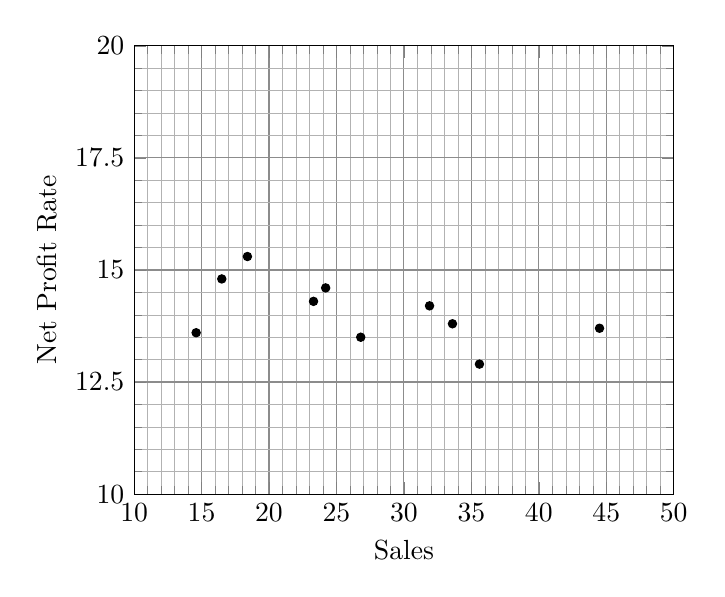
\begin{tikzpicture}
                        \begin{axis}[
                            xlabel=Sales,
                            ylabel=Net Profit Rate,
                            xmin=10, xmax=50,
                            ymin=10, ymax=20,
                            xtick={10, 15, ..., 50},
                            ytick={10, 12.5, ..., 20},
                            grid=both,
                            grid style={line width=.2pt, draw=gray!60},
                            major grid style={line width=.4pt,draw=gray!90},
                            minor tick num=4,
                          ]
                          \addplot[mark=*, mark size=1.5, mark options={solid, fill=black}, only marks] coordinates {(18.4, 15.3) (16.5, 14.8) (14.6, 13.6) (23.3, 14.3) (35.6, 12.9) (24.2, 14.6) (33.6, 13.8) (44.5, 13.7) (26.8, 13.5) (31.9, 14.2)};
                        \end{axis}
                      \end{tikzpicture}
                    }
                  \end{center}

            \item Find the correlation coefficient of the sales and the net profit rate, and
                  determine on the strength of the correlation. \sol{}
                  \begin{center}
                    \resizebox{\columnwidth-4.6em}{!}{
                      \begin{tabular}{|c|c|c|c|c|}
                        \hline
                        $x_i$       & $y_i$       & $x_i^2$       & $y_i^2$       & $x_iy_i$       \\
                        \hline
                        18.4        & 15.3        & 338.56        & 234.09        & 281.52         \\
                        16.5        & 14.8        & 272.25        & 219.04        & 244.2          \\
                        14.6        & 13.6        & 213.16        & 184.96        & 198.56         \\
                        23.3        & 14.3        & 542.89        & 204.49        & 333.19         \\
                        35.6        & 12.9        & 1267.36       & 166.41        & 459.24         \\
                        24.2        & 14.6        & 585.64        & 213.16        & 353.32         \\
                        33.6        & 13.8        & 1128.96       & 190.44        & 463.68         \\
                        44.5        & 13.7        & 1980.25       & 187.69        & 609.65         \\
                        26.8        & 13.5        & 718.24        & 182.25        & 361.8          \\
                        31.9        & 14.2        & 1017.61       & 201.64        & 452.98         \\
                        \hline
                        \hline
                        $\sum{x_i}$ & $\sum{y_i}$ & $\sum{x_i^2}$ & $\sum{y_i^2}$ & $\sum{x_iy_i}$ \\
                        \hline
                        269.4       & 140.7       & 8064.92       & 1984.17       & 3758.14        \\
                        \hline
                      \end{tabular}
                    }
                  \end{center}
                  \begin{flalign*}
                    \bar{x}                                                     & = \frac{269.4}{10} = 26.94                                                     \\
                    \bar{y}                                                     & = \frac{140.7}{10} = 14.07                                                     \\
                    r                                                           & = \frac{\frac{3758.14}{10} - 26.94 \cdot 14.07}{\sqrt{\left(\frac{8064.92}{10}
                    - 26.94^2\right)\left(\frac{1984.17}{10} - 14.07^2\right)}} &                                                                                \\
                                                                                & = -0.5350
                  \end{flalign*}
                  According to the result of the calculation, the sales and the net profit rate are negatively and moderately correlated.

          \end{enumerate}

  \end{enumerate}

  \section{Statistical Index}

  \subsection*{Index}

  In statistics, an index is a number that measures the changes in a figure from
  one point in time to another. There is a wide range of applications of an
  index, such as the price index which represents the changes in prices, the
  production index which represents the changes in production, and the wage index
  which represents the changes in salaries and wages. There are also other
  indices such as the living index, foreign exchange index, population index,
  stock market index, etc.

  The index is a kind of relative number. The standard period that is used for
  comparison when calculating the index is called the base period. As the case
  may be, the base period can be a year or a month. The index of the base period
  is usually a number that is easier to be remembered and compared, such as 100,
  500, or 1000, and the chosen number must be able to represent the changes in
  the figure. We will use 100 as our base period index. The period that is used
  for comparison to the base period is called the current period. Let $Q_0$ be
  the base period index and $Q_1$ be the current period index. The index of the
  current period is calculated by the following formula:

  \begin{cequation}
    I = \frac{Q_1}{Q_0} \cdot 100
  \end{cequation}

  \noindent where 100 is the base period index.

  \subsection*{Relative price}

  The relative price is a simple index that compares the prices of products in
  different periods. Let $P_0$ be the price of a product in the base period and
  $P_1$ be the price of the same product in the current period. The price
  relative of the current period is calculated by the following formula:

  \begin{cequation}
    I = \frac{P_1}{P_0} \cdot 100
  \end{cequation}

  \subsection{Practice 11}

  The table below shows the net profits (in million) of a company from 2010 to
  2014. Use the year 2010 as the base period and calculate the index of the net
  profit of the company in each year.
  \begin{center}
    \begin{tabular}{|c|c|c|c|c|c|}
      \hline
      Year       & 2010 & 2011 & 2012  & 2013  & 2014 \\
      \hline
      Net Profit & 700  & 621  & 584.1 & 720.5 & 800  \\
      \hline
    \end{tabular}
  \end{center}

  \sol{}
  \begin{flalign*}
    I_{2011} & = \frac{621}{700} \cdot 100 = 88.71    \\
    I_{2012} & = \frac{584.1}{700} \cdot 100 = 83.44  \\
    I_{2013} & = \frac{720.5}{700} \cdot 100 = 102.93 \\
    I_{2014} & = \frac{800}{700} \cdot 100 = 114.29
  \end{flalign*}

  \subsection{Exercise 18.7a}

  \begin{enumerate}
    \item The prices of white sugar in 2011, 2012, and 2013 are \$2.10, \$2.30, and
          \$2.50 respectively. Use the year 2011 and 2012 as the base period and
          calculate the relative price of the year 2013. \sol{}
          \begin{flalign*}
            P.R.\text{ with respect to 2011} & = \frac{2.50}{2.10} \cdot 100 = 119.05 & \\
            P.R.\text{ with respect to 2012} & = \frac{2.50}{2.30} \cdot 100 = 108.70
          \end{flalign*}

    \item The prices of a food product in 2011, 2013, and 2015 are \$3.40, \$3.75, and
          \$3.90 respectively. Use the year 2011 as the base period and calculate the
          relative price of the year 2013 and 2015. \sol{}
          \begin{flalign*}
            P.R.\text{ of 2013} & = \frac{3.75}{3.40} \cdot 100 = 110.29 & \\
            P.R.\text{ of 2015} & = \frac{3.90}{3.40} \cdot 100 = 114.71
          \end{flalign*}

    \item The number of new students of a school from 2011 to 2015 are as follows:
          \begin{center}
            \begin{tabular}{|c|c|c|c|c|c|}
              \hline
              Year      & 2011 & 2012 & 2013 & 2014 & 2015 \\
              \hline
              New Stud. & 182  & 150  & 120  & 104  & 94   \\
              \hline
            \end{tabular}
          \end{center}
          Use the year 2011 as the base period and calculate the index of the number of new students in each year.
          \sol{}
          \begin{flalign*}
            \text{New Stud. Index of 2012} & = \frac{150}{182} \cdot 100 = 82.42 & \\
            \text{New Stud. Index of 2013} & = \frac{120}{182} \cdot 100 = 65.93 & \\
            \text{New Stud. Index of 2014} & = \frac{104}{182} \cdot 100 = 57.14 & \\
            \text{New Stud. Index of 2015} & = \frac{94}{182} \cdot 100 = 51.64
          \end{flalign*}

    \item The table below shows the price of terraced houses (in \$10k) of a place in
          from 2019 to 2014:
          \begin{center}
            \begin{tabular}{|c|c|c|c|c|c|}
              \hline
              Year  & 2010 & 2011 & 2012 & 2013 & 2014 \\
              \hline
              Price & 32.0 & 35.5 & 43.4 & 51.0 & 60.0 \\
              \hline
            \end{tabular}
          \end{center}
          Use the year 2010 as the base period and calculate the relative price of terraced houses in each year.
          \sol{}
          \begin{flalign*}
            P.R.\text{ of 2011} & = \frac{35.5}{32.0} \cdot 100 = 110.94 & \\
            P.R.\text{ of 2012} & = \frac{43.4}{32.0} \cdot 100 = 135.63 & \\
            P.R.\text{ of 2013} & = \frac{51.0}{32.0} \cdot 100 = 159.38 & \\
            P.R.\text{ of 2014} & = \frac{60.0}{32.0} \cdot 100 = 187.50
          \end{flalign*}

    \item The table below shows the relative price of three products $A$, $B$, and $C$
          when using different years as the base period and the current period:
          \begin{center}
            \begin{tabular}{|c|c|c|c|c|}
              \hline
              Current Period & Base Period & $A$ & $B$ & $C$ \\
              \hline
              2010           & 2005        & 160 & $x$ & 170 \\
              2015           & 2005        & 140 & 190 & $y$ \\
              2015           & 2010        & $z$ & 210 & 150 \\
              \hline
            \end{tabular}
          \end{center}
          Find the value of $x$, $y$, and $z$.
          \sol{}

          Let the price of $A$ in 2005, 2010, and 2015 be $a = 100$, $b$, and $c$
          respectively. From the statement above, we have
          \begin{flalign*}
            \frac{b}{a} \cdot 100 & = \frac{b}{100} \cdot 100   \\
            b                     & = 160                       \\
            \frac{c}{b} \cdot 100 & = \frac{c}{160} \cdot 100   \\
            c                     & = 140                       \\
            z                     & = \frac{c}{b} \cdot 100     \\
                                  & = \frac{140}{160} \cdot 100 \\
                                  & = 87.5
          \end{flalign*}

          Let the price of $B$ in 2005, 2010, and 2015 be $a$, $b$, and $c = 100$
          respectively. From the statement above, we have
          \begin{flalign*}
            \frac{c}{a} \cdot 100   & = \frac{100}{a} \cdot 100                         \\
            \frac{100}{a} \cdot 100 & = 190                                             \\
            1.9a                    & = 100                                             \\
            a                       & = \frac{100}{1.9}                                 \\
            \frac{c}{b} \cdot 100   & = \frac{100}{b} \cdot 100                         \\
            \frac{100}{b} \cdot 100 & = 210                                             \\
            2.1b                    & = 100                                             \\
            b                       & = \frac{100}{2.1}                                 \\
            x                       & = \frac{b}{a} \cdot 100                           \\
                                    & = \frac{100}{2.1} \cdot \frac{1.9}{100} \cdot 100 \\
                                    & = \frac{1.9}{2.1} \cdot 100                       \\
                                    & = 90.48
          \end{flalign*}

          Let the price of $C$ in 2005, 2010, and 2015 be $a$, $b = 100$, and $c$
          respectively. From the statement above, we have
          \begin{flalign*}
            \frac{b}{a} \cdot 100     & = \frac{100}{a} \cdot 100             \\
            \frac{100}{a} \cdot 100   & = 170                                 \\
            1.7a                      & = 100                                 \\
            a                         & = \frac{100}{1.7}                     \\
            \frac{c}{b} \cdot 100     & = \frac{c}{100} \cdot 100             \\
            c                         & = 150                                 \\
            y                         & = \frac{c}{a} \cdot 100               \\
                                      & = 150 \cdot \frac{1.7}{100} \cdot 100 \\
                                      & = 255                                 \\
            \\
            \therefore\ x = 90.48,\ y & = 255,\ z = 87.5
          \end{flalign*}

  \end{enumerate}

  \subsection*{Composite Index}

  The composite index is the mean value of indices of different figures. Since
  the importance of each figure might be different, the weight of each index is
  used to represent the importance of each figure, and the acquired weighted mean
  is called the composite index.

  Let the simple index of $n$ figures of the same base period and the same
  current period be $x_1, x_2, \ldots, x_n$, and their respective weights be
  $w_1, w_2, \ldots, w_n$. The composite index is calculated by the following
  formula:

  \makeatletter
  \setbool{@fleqn}{false}
  \makeatother
  \begin{flalign*}
    \text{Composite Index} & = \frac{w_1x_1 + w_2x_2 + \cdots + w_nx_n}{w_1 + w_2 + \cdots + w_n} \\
                           & = \frac{\sum{w_ix_i}}{\sum{w_i}}
  \end{flalign*}
  \makeatletter
  \setbool{@fleqn}{true}
  \makeatother

  If the study object is some product, where $x_i$ is the relative price to the
  $i^{th}$ product, then its weighted mean is called the price index. If the
  study object is the daily living expenses, then its weighted mean is called the
  living consumption index.

  \subsection{Practice 12}

  The table below shows the prices and weights of sneakers of three brands in
  2012 and 2015:
  \begin{center}
    \begin{tabular}{|c|c|c|c|}
      \hline
      \multirow{2}{*}{Sneakers} & \multicolumn{2}{c|}{Unit Price} & \multirow{2}{*}{Weight}     \\
      \cline{2-3}
                                & 2012                            & 2015                    &   \\
      \hline
      A                         & 230                             & 233                     & 5 \\
      B                         & 225                             & 228                     & 3 \\
      C                         & 215                             & 221                     & 2 \\
      \hline
    \end{tabular}
  \end{center}
  \begin{enumerate}
    \item Use the year 2012 as the base period and calculate the relative price of each
          brand in 2015. \sol{}
          \begin{flalign*}
            P.R. \text{ of } A & = \frac{233}{230} \cdot 100 = 101.30 \\
            P.R. \text{ of } B & = \frac{228}{225} \cdot 100 = 101.33 \\
            P.R. \text{ of } C & = \frac{221}{215} \cdot 100 = 102.79
          \end{flalign*}

    \item Use the year 2012 as the base period and calculate the price index of sneakers
          in 2015. \sol{}
          \begin{center}
            \begin{tabular}{|c|c|c|c|}
              \hline
              Sneakers & P.R. $x_i$ & Weight $w_i$ & $w_ix_i$       \\
              \hline
              A        & 101.30     & 5            & 506.5          \\
              B        & 101.33     & 3            & 303.99         \\
              C        & 102.79     & 2            & 205.58         \\
              \hline
              \hline
                       &            & $\sum w_i$   & $\sum{w_ix_i}$ \\
                       &            & 10           & 1016.07        \\
              \hline
            \end{tabular}
          \end{center}
          \begin{flalign*}
            \text{Price Index} & = \frac{1016.07}{10} \\
                               & = 101.61
          \end{flalign*}
  \end{enumerate}

  \subsection{Exercise 18.7b}

  \begin{enumerate}
    \item Using 2012 as the base period, the relative prices of foods, gases and clothes
          in 2014 are 111, 105, and 106 respectively, and their weights are 5, 1, and 2
          respectively. Calculate the composite index of the three comsumer items in
          2014. \sol{}
          \begin{center}
            \begin{tabular}{|c|c|c|c|}
              \hline
              Item  & P.R. $x_i$ & Weight $w_i$ & $w_ix_i$       \\
              \hline
              Food  & 111        & 5            & 555            \\
              Gas   & 105        & 1            & 105            \\
              Cloth & 106        & 2            & 212            \\
              \hline
              \hline
                    &            & $\sum w_i$   & $\sum{w_ix_i}$ \\
              \hline
                    &            & 8            & 872            \\
              \hline
            \end{tabular}
          \end{center}
          \begin{flalign*}
            \text{Composite Index} & = \frac{872}{8} \\
                                   & = 109
          \end{flalign*}

    \item The table below shows the price of each primary food in 2015 (with 2005 as the
          base period). Find the price index in 2015.
          \begin{center}
            \begin{tabular}{|c|c|c|}
              \hline
              Food        & Relative price & Weight \\
              \hline
              Meat        & 130            & 15     \\
              Fish        & 150            & 14     \\
              Vegetable   & 200            & 10     \\
              Rice        & 110            & 20     \\
              Cooking Oil & 120            & 8      \\
              Beverage    & 150            & 7      \\
              Fruit       & 160            & 6      \\
              \hline
            \end{tabular}
          \end{center}
          \sol{}
          \begin{center}
            \begin{tabular}{|c|c|c|c|}
              \hline
              Food        & P.R. $x_i$ & Weight $w_i$ & $w_ix_i$       \\
              \hline
              Meat        & 130        & 15           & 1950           \\
              Fish        & 150        & 14           & 2100           \\
              Vegetable   & 200        & 10           & 2000           \\
              Rice        & 110        & 20           & 2200           \\
              Cooking Oil & 120        & 8            & 960            \\
              Beverage    & 150        & 7            & 1050           \\
              Fruit       & 160        & 6            & 960            \\
              \hline
              \hline
                          &            & $\sum w_i$   & $\sum{w_ix_i}$ \\
              \hline
                          &            & 80           & 11200          \\
              \hline
            \end{tabular}
          \end{center}
          \begin{flalign*}
            \text{Price Index} & = \frac{11200}{80} \\
                               & = 140.25
          \end{flalign*}

    \item The weight and unit price of 3 kind of materials bought by a factory are as
          follows:
          \begin{center}
            \begin{tabular}{|c|c|c|c|}
              \hline
              \multirow{2}{*}{Material} & \multirow{2}{*}{Weight (ton)} & \multicolumn{2}{c|}{Unit Price (\$)}        \\
              \cline{3-4}
                                        &                               & 2010                                 & 2014 \\
              \hline
              A                         & 20                            & 0.62                                 & 0.71 \\
              B                         & 50                            & 2.05                                 & 2.09 \\
              C                         & 60                            & 0.80                                 & 0.85 \\
              \hline
            \end{tabular}
          \end{center}
          Using 2010 as the base period, 2014 as the current period,
          \begin{enumerate}
            \item Find the composite index of the unit prices of the three materials without
                  considering the weights (i.e. the weights are all 1). \sol{}
                  \begin{flalign*}
                    P.R. \text{ of } A & = \frac{0.71}{0.62} \cdot 100 \\
                                       & = 114.52                      \\
                    P.R. \text{ of } B & = \frac{2.09}{2.05} \cdot 100 \\
                                       & = 101.95                      \\
                    P.R. \text{ of } C & = \frac{0.85}{0.80} \cdot 100 \\
                                       & = 106.25
                  \end{flalign*}
                  \begin{center}
                    \begin{tabular}{|c|c|c|c|}
                      \hline
                      Material & P.R. $x_i$ & Weight $w_i$ & $w_ix_i$       \\
                      \hline
                      A        & 114.52     & 1            & 114.52         \\
                      B        & 101.95     & 1            & 101.95         \\
                      C        & 106.25     & 1            & 106.25         \\
                      \hline
                      \hline
                               &            & $\sum w_i$   & $\sum{w_ix_i}$ \\
                      \hline
                               &            & 3            & 322.72         \\
                      \hline
                    \end{tabular}
                  \end{center}
                  \begin{flalign*}
                    \text{Composite Index} & = \frac{322.72}{3} \\
                                           & = 107.57
                  \end{flalign*}

            \item Using the weight of each material as the weight, find the composite index of
                  the unit prices of the three materials. \sol{}
                  \begin{center}
                    \begin{tabular}{|c|c|c|c|}
                      \hline
                      Material & P.R. $x_i$ & Weight $w_i$ & $w_ix_i$       \\
                      \hline
                      A        & 114.52     & 20           & 2290.4         \\
                      B        & 101.95     & 50           & 5097.5         \\
                      C        & 106.25     & 60           & 6375           \\
                      \hline
                      \hline
                               &            & $\sum w_i$   & $\sum{w_ix_i}$ \\
                      \hline
                               &            & 130          & 13762.9        \\
                      \hline
                    \end{tabular}
                  \end{center}
                  \begin{flalign*}
                    \text{Composite Index} & = \frac{13762.9}{130} \\
                                           & = 105.87
                  \end{flalign*}
          \end{enumerate}

    \item The table below shows three indices and their weights. If their composite index
          is 103, find the value of $x$.
          \begin{center}
            \begin{tabular}{|c|c|c|c|}
              \hline
              Index  & 90  & 11$x$ & 120 \\
              \hline
              Weight & $x$ & 4     & 6   \\
              \hline
            \end{tabular}
          \end{center}
          \sol{}
          \begin{flalign*}
            \frac{x \cdot 90 + 4 \cdot 11 + 6 \cdot 120}{x + 4 + 6} & = 103         \\
            \frac{90x + 44x + 720}{x + 10}                          & = 103         \\
            134x + 720                                              & = 103x + 1030 \\
            31x                                                     & = 310         \\
            x                                                       & = 10
          \end{flalign*}

    \item The table below shows the relative price and weight of three products with 2013
          as the base period and 2015 as the current period. Given that the price of item
          $A$ in 2013 and 2015 are $\$20$ and $\$25$ respectively, the price relative of
          item $B$ is twice the price of item $A$.
          \begin{center}
            \begin{tabular}{|c|c|c|}
              \hline
              Item & Relative price & Weight \\
              \hline
              A    & $r$            & 2      \\
              B    & $t$            & 1      \\
              C    & 120            & 3      \\
              \hline
            \end{tabular}
          \end{center}
          \begin{enumerate}
            \item Find the value of $r$ adn $t$.
                  \begin{flalign*}
                    r & = \frac{25}{20} \cdot 100 \\
                      & = 125                     \\
                    t & = 2 \cdot 125             \\
                      & = 250
                  \end{flalign*}
            \item Using 2013 as the base period, find the price index in 2015. \sol{}
                  \begin{center}
                    \begin{tabular}{|c|c|c|c|}
                      \hline
                      Item & P.R. $x_i$ & Weight $w_i$ & $w_ix_i$       \\
                      \hline
                      A    & 125        & 2            & 250            \\
                      B    & 250        & 1            & 250            \\
                      C    & 120        & 3            & 360            \\
                      \hline
                      \hline
                           &            & $\sum w_i$   & $\sum{w_ix_i}$ \\
                      \hline
                           &            & 6            & 860            \\
                      \hline
                    \end{tabular}
                  \end{center}
                  \begin{flalign*}
                    \text{Price Index} & = \frac{860}{6} \\
                                       & = 143.33
                  \end{flalign*}
          \end{enumerate}

    \item The table below shows the relative price and weight of 5 products with 2012 as
          the base period and 2014 as the current period:
          \begin{center}
            \begin{tabular}{|c|c|c|}
              \hline
              Item & Relative price & Weight \\
              \hline
              A    & 125            & 2      \\
              B    & 120            & 3$x$   \\
              C    & 110            & 2      \\
              D    & 130            & $x$    \\
              E    & 115            & 2      \\
              \hline
            \end{tabular}
          \end{center}
          Given that the price index in 2014 is 120,
          \begin{enumerate}
            \item Find the value of $x$. \sol{}
                  \begin{flalign*}
                    \frac{2 \cdot 125 + 3x \cdot 120 + \cdots + 2 \cdot 115}{2 + 3x + 2 + x + 2} & = 120        & \\
                    \frac{250 + 360x + 220 + 130x + 230}{6 + 4x}                                 & = 120          \\
                    \frac{125 + 180x + 110 + 65x + 115}{3 + 2x}                                  & = 120          \\
                    350 + 245x                                                                   & = 360 + 240x   \\
                    5x                                                                           & = 10           \\
                    x                                                                            & = 2
                  \end{flalign*}
            \item Assume that the price of item $A$ in 2014 is \$30, find the price of the item
                  in 2012. \sol{}

                  Let the price of item $A$ in 2012 be $x$.
                  \begin{flalign*}
                    \frac{30}{x} \cdot 100 & = 125  \\
                    125x                   & = 3000 \\
                    x                      & = 24
                  \end{flalign*}
                  Therefore, the price of item $A$ in 2012 is \$24.
          \end{enumerate}

    \item The table below shows the price, relative price and weight of 4 products in
          2012 and 2014:
          \begin{center}
            \begin{tabular}{|c|c|c|c|c|}
              \hline
              \multirow{2}{*}{Item} & \multicolumn{2}{c|}{Price (\$)} & \multirow{2}{*}{Relative price} & \multirow{2}{*}{Weight}     \\
              \cline{2-3}
                                    & 2012                            & 2014                            &                         &   \\
              \hline
              A                     & 12                              & $y$                             & 150                     & 1 \\
              B                     & $x$                             & 24                              & 120                     & 2 \\
              C                     & 14                              & 28                              & $z$                     & 3 \\
              D                     & 10                              & 13                              & 130                     & 4 \\
              \hline
            \end{tabular}
          \end{center}
          where the base period of the relative price is 2012, and the current period is 2014.
          \begin{enumerate}
            \item Find the value of $x$, $y$ and $z$. \sol{}
                  \begin{flalign*}
                    \frac{y}{12} \cdot 100   & = 150                      \\
                    y                        & = \frac{150 \cdot 12}{100} \\
                                             & = 18
                    \\
                    \frac{24}{x} \cdot 100   & = 120                      \\
                    120x                     & = 2400                     \\
                    x                        & = 20
                    \\
                    z                        & = \frac{28}{14} \cdot 100  \\
                                             & = 200                      \\
                    \\
                    \therefore\ x  = 20, \ y & = 18, \ z  = 200
                  \end{flalign*}

            \item Using 2012 as the base period, find the price index in 2014. \sol{}
                  \begin{center}
                    \begin{tabular}{|c|c|c|c|}
                      \hline
                      Item & P.R. $x_i$ & Weight $w_i$ & $w_ix_i$       \\
                      \hline
                      A    & 150        & 1            & 150            \\
                      B    & 120        & 2            & 240            \\
                      C    & 200        & 3            & 600            \\
                      D    & 130        & 4            & 520            \\
                      \hline
                      \hline
                           &            & $\sum w_i$   & $\sum{w_ix_i}$ \\
                      \hline
                           &            & 10           & 1510           \\
                      \hline
                    \end{tabular}
                  \end{center}
                  \begin{flalign*}
                    \text{Price Index} & = \frac{1510}{10} \\
                                       & = 151
                  \end{flalign*}
          \end{enumerate}

    \item The table below shows the price of two products in 2005 and 2015:
          \begin{center}
            \begin{tabular}{|c|c|c|c|}
              \hline
              \multirow{2}{*}{Item} & \multicolumn{2}{c|}{Price (\$)} & \multirow{2}{*}{Relative price}     \\
              \cline{2-3}
                                    & 2005                            & 2015                            &   \\
              \hline
              A                     & 30                              & $x$                             & 2 \\
              B                     & 50                              & $x+10$                          & 3 \\
              \hline
            \end{tabular}
          \end{center}
          Using 2005 as base period,
          \begin{enumerate}
            \item Assume that the price relative of these two items are the same in 2015, find
                  the value of $x$. \sol{}
                  \begin{flalign*}
                    \frac{x}{30} \cdot 100 & = \frac{x+10}{50} \cdot 100 \\
                    \frac{x}{30}           & = \frac{x+10}{50}           \\
                    50x                    & = 30x + 300                 \\
                    20x                    & = 300                       \\
                    x                      & = 15
                  \end{flalign*}
            \item Find the price index of these two items in 2015. \sol{}
                  \begin{flalign*}
                    \text{Price index} & = \frac{15}{30} \cdot 100 \\
                                       & = 50
                  \end{flalign*}
                  \begin{center}
                    \begin{tabular}{|c|c|c|c|}
                      \hline
                      Item & P.R. $x_i$ & Weight $w_i$ & $w_ix_i$       \\
                      \hline
                      A    & 50         & 2            & 100            \\
                      B    & 50         & 3            & 150            \\
                      \hline
                      \hline
                           &            & $\sum w_i$   & $\sum{w_ix_i}$ \\
                      \hline
                           &            & 5            & 250            \\
                      \hline
                    \end{tabular}
                  \end{center}
                  \begin{flalign*}
                    \text{Price Index} & = \frac{250}{5} \\
                                       & = 50
                  \end{flalign*}
          \end{enumerate}

  \end{enumerate}

  \section{Revision Exercise 18}

  \begin{enumerate}
    \item The length of 60 cotten fibers (in $mm$) in a laboratory are as follows:
          \begin{flalign*}
            82  & \quad 202 \quad 352 \quad 321 \quad 25 \quad 293 \quad 293 \quad 86   & \\
            28  & \quad 206 \quad 323 \quad 355 \quad 357 \quad 33 \quad 325 \quad 113  & \\
            233 & \quad 294 \quad 50 \quad 296 \quad 115 \quad 236 \quad 357 \quad 326  & \\
            52  & \quad 301 \quad 140 \quad 328 \quad 238 \quad 358 \quad 58 \quad 255  & \\
            143 & \quad 360 \quad 340 \quad 302 \quad 370 \quad 343 \quad 260 \quad 303 & \\
            59  & \quad 146 \quad 60 \quad 263 \quad 170 \quad 175 \quad 348 \quad 305  & \\
            380 & \quad 346 \quad 61 \quad 305 \quad 264 \quad 383 \quad 62 \quad 306   & \\
            195 & \quad 350 \quad 265 \quad 385
          \end{flalign*}
          \begin{enumerate}
            \item Using $21mm$ as the lower limit and $40mm$ as the class range, construct a
                  frequency distribution table. \sol{}
                  \begin{center}
                    \begin{tabular}{|c|c|}
                      \hline
                      Length    & Frequency \\
                      \hline
                      21 - 60   & 8         \\
                      61 - 100  & 4         \\
                      101 - 140 & 3         \\
                      141 - 180 & 4         \\
                      181 - 220 & 3         \\
                      221 - 260 & 5         \\
                      261 - 300 & 7         \\
                      301 - 340 & 12        \\
                      341 - 380 & 12        \\
                      381 - 420 & 2         \\
                      \hline
                    \end{tabular}
                  \end{center}
            \item Construct a histogram and a frequency polygon. \sol{}
                  \begin{center}
                    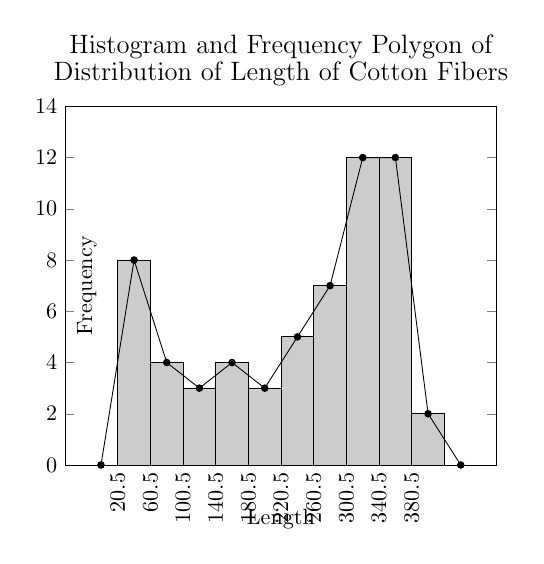
\begin{tikzpicture}[scale=0.8]
                      \begin{axis}[
                          title style = {align = center},
                          title={\large{Histogram and Frequency Polygon of} \\ \large{Distribution of Length of Cotton Fibers}},
                          ymin=0, ymax=14,
                          ytick={0, 2, ..., 14},
                          xtick={20.5, 60.5, 100.5, 140.5, 180.5, 220.5, 260.5, 300.5, 340.5, 380.5},
                          grid=none,
                          xtick style={draw=none, fill=none, font=\footnotesize},
                          x tick label style = {rotate=90,anchor=east},
                          xlabel=Length=, ylabel=Frequency,
                          xlabel style={at={(axis description cs:0.5, -0.1)}, anchor=north},
                          ylabel style={at={(axis description cs:0.05, 0.5)}, anchor=center},
                        ]
                        \addplot[ybar interval, draw=black, style={fill=gray!40},mark=no] plot coordinates { (20.5, 8) (60.5, 4) (100.5, 3) (140.5, 4) (180.5, 3) (220.5, 5) (260.5, 7) (300.5, 12) (340.5, 12) (380.5, 2) (420.5, 0) };
                        \addplot[forget plot, sharp plot, mark=*, mark size=1.5pt, mark options={solid, fill=black, draw=black}, draw=black]
                        coordinates
                          { (0, 0) (40.5, 8) (80.5, 4) (120.5, 3) (160.5, 4) (200.5, 3) (240.5, 5) (280.5, 7) (320.5, 12) (360.5, 12) (400.5, 2) (440.5, 0) };
                      \end{axis}
                    \end{tikzpicture}
                  \end{center}

            \item Construct a cumulative frequency table and a cumulative frequency polygon.
                  \sol{}
                  \begin{center}
                    \resizebox{\columnwidth-4.6em}{!}{
                      \begin{tabular}{|c|c|c|c|}
                        \hline
                        Range     & Freq. & Lower Than & Cum. Freq. \\
                        \hline
                        21 - 60   & 8     & 60.5       & 8          \\
                        61 - 100  & 4     & 100.5      & 12         \\
                        101 - 140 & 3     & 140.5      & 15         \\
                        141 - 180 & 4     & 180.5      & 19         \\
                        181 - 220 & 3     & 220.5      & 22         \\
                        221 - 260 & 5     & 260.5      & 27         \\
                        261 - 300 & 7     & 300.5      & 34         \\
                        301 - 340 & 12    & 340.5      & 46         \\
                        341 - 380 & 12    & 380.5      & 58         \\
                        381 - 420 & 2     & 420.5      & 60         \\
                        \hline
                      \end{tabular}
                    }
                  \end{center}

                  \begin{center}
                    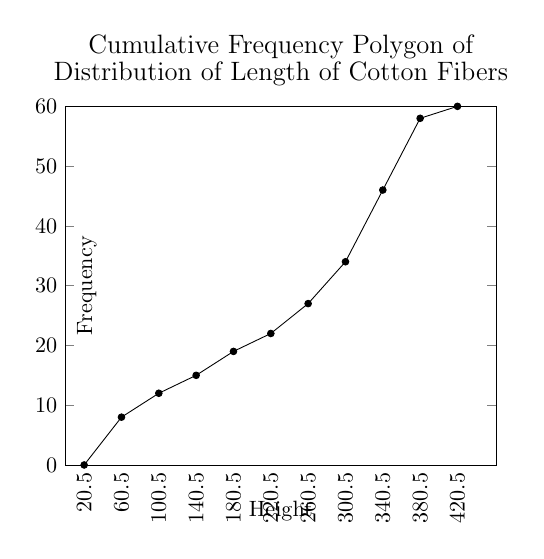
\begin{tikzpicture}[scale=0.8]
                      \begin{axis}[
                          title style = {align = center},
                          title={\large{Cumulative Frequency Polygon of} \\ \large{Distribution of Length of Cotton Fibers}},
                          ymin=0, ymax=60,
                          xmin=0,
                          ytick={0, 10, ..., 60},
                          xtick={20.5, 60.5, 100.5, 140.5, 180.5, 220.5, 260.5, 300.5, 340.5, 380.5, 420.5},
                          xtick style={draw=none, fill=none, font=\footnotesize}, x tick label style =
                            {rotate=90,anchor=east}, xlabel=Height, ylabel=Frequency, xlabel style={at={(axis
                                  description cs:0.5, -0.08)}, anchor=north}, ylabel style={at={(axis
                                  description cs:0.05, 0.5)}, anchor=center}, ] \addplot[forget plot, sharp
                          plot, mark=*, mark size=1.5pt, mark options={solid, fill=black, draw=black},
                          draw=black] coordinates { (20.5, 0) (60.5, 8) (100.5, 12) (140.5, 15) (180.5, 19) (220.5, 22) (260.5, 27) (300.5, 34) (340.5, 46) (380.5, 58) (420.5, 60) };
                      \end{axis}
                    \end{tikzpicture}
                  \end{center}

            \item Using the cumulative frequency polygon, find the percentage of fibers whose
                  length is greater than $150mm$. \sol{}

                  \begin{center}
                    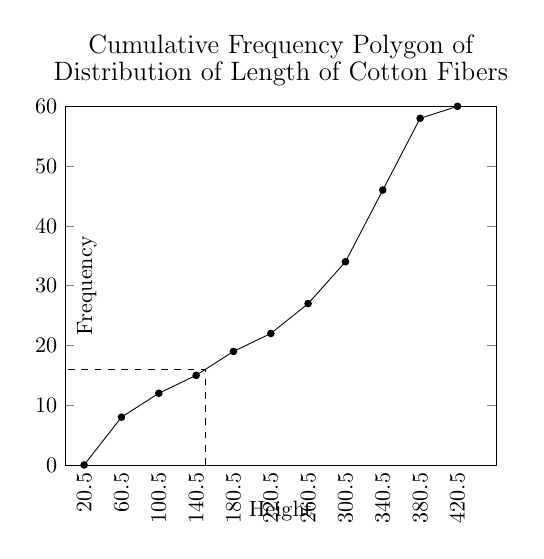
\begin{tikzpicture}[scale=0.8]
                      \begin{axis}[
                          title style = {align = center},
                          title={\large{Cumulative Frequency Polygon of} \\ \large{Distribution of Length of Cotton Fibers}},
                          ymin=0, ymax=60,
                          xmin=0,
                          ytick={0, 10, ..., 60},
                          xtick={20.5, 60.5, 100.5, 140.5, 180.5, 220.5, 260.5, 300.5, 340.5, 380.5, 420.5},
                          xtick style={draw=none, fill=none, font=\footnotesize}, x tick label style =
                            {rotate=90,anchor=east}, xlabel=Height, ylabel=Frequency, xlabel style={at={(axis
                                  description cs:0.5, -0.08)}, anchor=north}, ylabel style={at={(axis
                                  description cs:0.05, 0.5)}, anchor=center}, ] \addplot[forget plot, sharp
                          plot, mark=*, mark size=1.5pt, mark options={solid, fill=black, draw=black},
                          draw=black] coordinates { (20.5, 0) (60.5, 8) (100.5, 12) (140.5, 15) (180.5, 19) (220.5, 22) (260.5, 27) (300.5, 34) (340.5, 46) (380.5, 58) (420.5, 60) };
                        \draw [dashed] (axis cs: 150, 0) -- (axis cs: 150, 16) -- (axis cs: 0, 16);
                      \end{axis}
                    \end{tikzpicture}
                  \end{center}

                  From the cumulative frequency polygon, there are 16 fibers whose length is less
                  than $150mm$, that is, there are $60 - 16 = 44$ fibers whose length is greater
                  than $150mm$. Therefore, the percentage of fibers whose length is greater than
                  $150mm$ is $\frac{44}{60} \cdot 100 = 73.33\%$.

            \item Find the interquartile range. \sol{}

                  $n = 60$, $\frac{n}{4} = 15$, the class that contains $Q_1$ is $141 - 180$, $C_1 = 40$, $L_1 = 140.5$, $F_1 = 15$, $f_1 = 4$,
                  \begin{flalign*}
                    Q_1 & = 140.5 + \frac{15 - 12}{3} \cdot 40 = 140.5
                  \end{flalign*}

                  $n = 60$, $\frac{3n}{4} = 45$, the class that contains $Q_3$ is $301 - 340$, $C_3 = 40$, $L_3 = 300.5$, $F_3 = 34$, $f_3 = 12$,
                  \begin{flalign*}
                    Q_3 & = 300.5 + \frac{45 - 34}{12} \cdot 40 = 337.17
                  \end{flalign*}

                  Therefore, the interquartile range is $Q_3 - Q_1 = 337.17 - 140.5 = 196.67$.

          \end{enumerate}

    \item Find the mean, median, range, quartile deviation, and mean deviation of the
          data $8, 10, 9, 12, 4, 4, 2$. \sol{}
          \begin{flalign*}
            \text{Mean} & = \frac{8 + 10 + 9 + 12 + 4 + 4 + 2}{7} \\
                        & = \frac{49}{7}                          \\
                        & = 7
          \end{flalign*}
          Rearranging the data, we get
          \[2 \quad \typel{4}{$Q_1 = 4$} \quad 4 \quad \typem{8}{$Q_2 = 8$} \quad 9 \quad \typel{10}{$Q_3 = 10$} \quad 12\]
          The range is $12 - 2 = 10$, the quartile deviation is $\frac{10 - 4}{2} =
            \frac{6}{2} = 3$.
          \begin{flalign*}
            \text{Mean Dev.} & = \frac{|8 - 7| + |10 - 7| + \cdots + |2 - 7|}{7} \\
                             & = \frac{1 + 3 + 2 + 5 + 3 + 3 + 5}{7}             \\
                             & = \frac{22}{7}                                    \\
                             & = 3.14
          \end{flalign*}
          Therefore, mean $= 7$, median $= 8$, range $= 10$, quartile deviation $= 3$, and mean deviation $= 3.14$.

    \item The weight (in $kg$) if 16 babies are as follows:
          \begin{flalign*}
            8 & \quad 9 \quad 10 \quad 9 \quad 8 \quad 7 \quad 9 \quad 10 \\
            9 & \quad 8 \quad 8 \quad 9 \quad 10 \quad 9 \quad 8 \quad 7
          \end{flalign*}
          Find the mean, meidan, mode, range, quartile deviation, mean deviation, and standard deviation of their weights.
          \sol{}
          \begin{flalign*}
            \text{Mean} & = \frac{8 + 9 + \cdots + 7}{16} \\
                        & = \frac{138}{16}                \\
                        & = 8.63
          \end{flalign*}
          Rearranging the data, we get
          \begin{flalign*}
            7 & \quad 7 \quad 8 \quad 8 \quad 8 \quad 8 \quad 8 \quad 9    \\
            9 & \quad 9 \quad 9 \quad 9 \quad 9 \quad 10 \quad 10 \quad 10
          \end{flalign*}
          $n = 16$, median is the average of the value at the $\frac{16}{2} = 8$th position the $\frac{16}{2} + 1 = 9$th position, that is, $\frac{9 + 9}{2} = 18$.

          The mode is $9$, which occurs at the highest frequency of $6$.

          The range is $10 - 7 = 3$.

          $Q_1$ is the average of the value at the $\frac{16}{4} = 4$th position and the $\frac{16}{4} + 1 = 5$th position, that is, $\frac{8 + 8}{2} = 8$.

          $Q_3$ is the average of the value at the $\frac{3 \cdot 16}{4} = 12$th position and the $\frac{3 \cdot 16}{4} + 1 = 13$th position, that is, $\frac{9 + 9}{2} = 9$.

          The quartile deviation is $\frac{9 - 8}{2} = \frac{1}{2} = 0.5$.

          \begin{flalign*}
            \text{Mean Dev.} & = \frac{|7 - 8.63| + \cdots + |10 - 8.63|}{16} \\
                             & = \frac{1.63 + 1.63 + \cdots + 1.37}{16}       \\
                             & = \frac{12.74}{16}                             \\
                             & = 0.80
          \end{flalign*}
          \begin{flalign*}
            \sigma^2 & = \frac{7^2 + 7^2 + \cdots + 10^2}{16} - \left(\frac{138}{16}\right)^2 \\
                     & = 0.8594                                                               \\
            \sigma   & = \sqrt{0.8594}                                                        \\
                     & = 0.93
          \end{flalign*}

    \item The table below shows the score distribution of business study minor test of
          senior 3 students in a high school:
          \begin{center}
            \begin{tabular}{|c|c|c|}
              \hline
              Marks & No. of Students \\
              \hline
              0-9   & 7               \\
              10-19 & 21              \\
              20-29 & 32              \\
              30-39 & 27              \\
              40-49 & 13              \\
              \hline
            \end{tabular}
          \end{center}
          \begin{enumerate}
            \item Construct a cumulative frequency distribution table. \sol{}
                  \begin{center}
                    \begin{tabular}{|c|c|c|c|}
                      \hline
                      Range & Freq. & Lower Than & Cum. Freq. \\
                      \hline
                      0-9   & 7     & 9.5        & 7          \\
                      10-19 & 21    & 19.5       & 28         \\
                      20-29 & 32    & 29.5       & 60         \\
                      30-39 & 27    & 39.5       & 87         \\
                      40-49 & 13    & 49.5       & 100        \\
                      \hline
                    \end{tabular}
                  \end{center}

            \item Construct a cumulative frequency polygon. \sol{}
                  \begin{center}
                    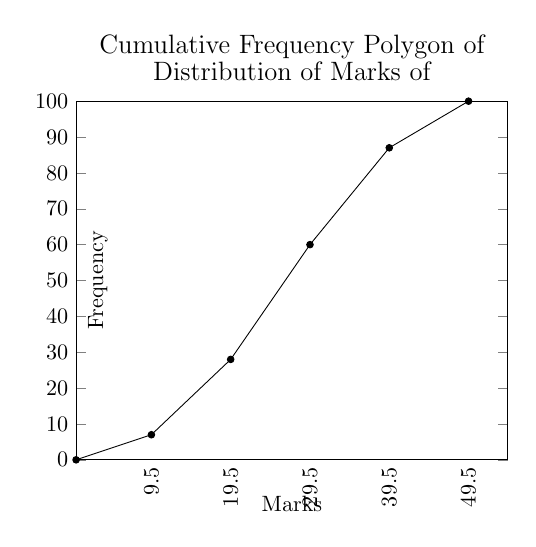
\begin{tikzpicture}[scale=0.8]
                      \begin{axis}[
                          title style = {align = center},
                          title={\large{Cumulative Frequency Polygon of} \\ \large{Distribution of Marks of}},
                          ymin=0, ymax=100,
                          xmin=0,
                          ytick={0, 10, ..., 100},
                          xtick={9.5, 19.5, ..., 49.5},
                          xtick style={draw=none, fill=none, font=\footnotesize}, x tick label style =
                            {rotate=90,anchor=east}, xlabel=Marks, ylabel=Frequency, xlabel style={at={(axis
                                  description cs:0.5, -0.08)}, anchor=north}, ylabel style={at={(axis
                                  description cs:0.05, 0.5)}, anchor=center}, ] \addplot[forget plot, sharp
                          plot, mark=*, mark size=1.5pt, mark options={solid, fill=black, draw=black},
                          draw=black] coordinates { (0.0, 0) (9.5, 7) (19.5, 28) (29.5, 60) (39.5, 87) (49.5, 100) (59.5, 120) };
                      \end{axis}
                    \end{tikzpicture}
                  \end{center}

            \item Find the median and the interquartile range from the cumulative frequency
                  polygon. \sol{}
                  \begin{center}
                    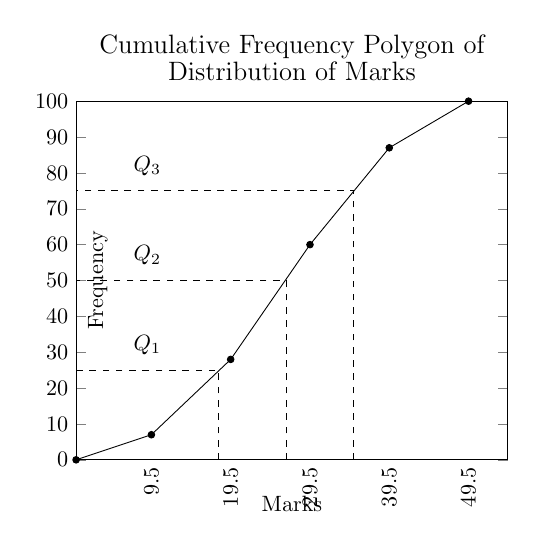
\begin{tikzpicture}[scale=0.8]
                      \begin{axis}[
                          title style = {align = center},
                          title={\large{Cumulative Frequency Polygon of} \\ \large{Distribution of Marks}},
                          ymin=0, ymax=100,
                          xmin=0,
                          ytick={0, 10, ..., 100},
                          xtick={9.5, 19.5, ..., 49.5},
                          xtick style={draw=none, fill=none, font=\footnotesize}, x tick label style =
                            {rotate=90,anchor=east}, xlabel=Marks, ylabel=Frequency, xlabel style={at={(axis
                                  description cs:0.5, -0.08)}, anchor=north}, ylabel style={at={(axis
                                  description cs:0.05, 0.5)}, anchor=center}, ] \addplot[forget plot, sharp
                          plot, mark=*, mark size=1.5pt, mark options={solid, fill=black, draw=black},
                          draw=black] coordinates { (0.0, 0) (9.5, 7) (19.5, 28) (29.5, 60) (39.5, 87) (49.5, 100) (59.5, 120) };
                        \draw [dashed] (axis cs: 26.5, 0) -- (axis cs: 26.5, 50) -- (axis cs: 0, 50);
                        \draw [dashed] (axis cs: 35, 0) -- (axis cs: 35, 75) -- (axis cs: 0, 75);
                        \draw [dashed] (axis cs: 18, 0) -- (axis cs: 18, 25) -- (axis cs: 0, 25);
                        \node at (axis cs: 9.0, 32) {$Q_1$};
                        \node at (axis cs: 9.0, 57) {$Q_2$};
                        \node at (axis cs: 9.0, 82) {$Q_3$};
                      \end{axis}
                    \end{tikzpicture}
                  \end{center}

            \item Find the percentage of students who scored higher or equal to 45 marks. \sol{}
                  \begin{center}
                    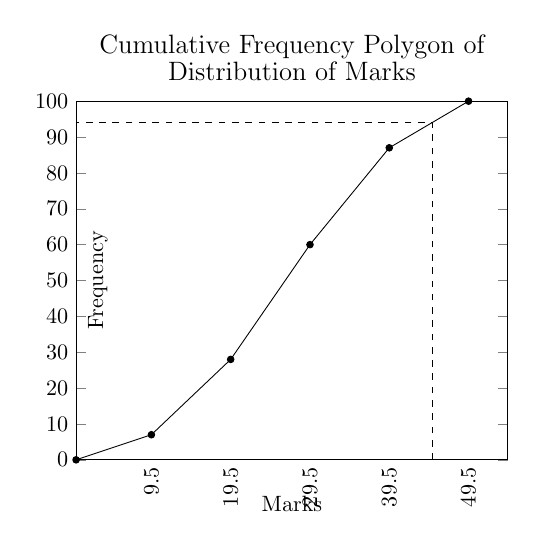
\begin{tikzpicture}[scale=0.8]
                      \begin{axis}[
                          title style = {align = center},
                          title={\large{Cumulative Frequency Polygon of} \\ \large{Distribution of Marks}},
                          ymin=0, ymax=100,
                          xmin=0,
                          ytick={0, 10, ..., 100},
                          xtick={9.5, 19.5, ..., 49.5},
                          xtick style={draw=none, fill=none, font=\footnotesize}, x tick label style =
                            {rotate=90,anchor=east}, xlabel=Marks, ylabel=Frequency, xlabel style={at={(axis
                                  description cs:0.5, -0.08)}, anchor=north}, ylabel style={at={(axis
                                  description cs:0.05, 0.5)}, anchor=center}, ] \addplot[forget plot, sharp
                          plot, mark=*, mark size=1.5pt, mark options={solid, fill=black, draw=black},
                          draw=black] coordinates { (0.0, 0) (9.5, 7) (19.5, 28) (29.5, 60) (39.5, 87) (49.5, 100) (59.5, 120) };
                        \draw [dashed] (axis cs: 45, 0) -- (axis cs: 45, 94) -- (axis cs: 0, 94);
                      \end{axis}
                    \end{tikzpicture}
                  \end{center}
                  From the diagram, we can see that there are 6 students who scored 45 marks or above.

            \item Assume that the passing score is 15 marks. Find the percentage of students who
                  failed the test.
                  \begin{center}
                    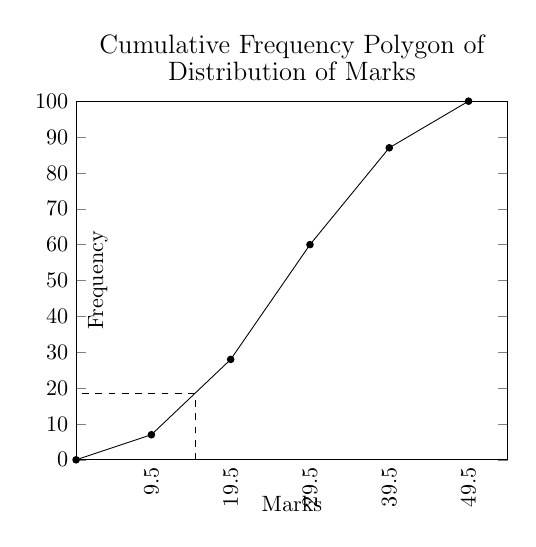
\begin{tikzpicture}[scale=0.8]
                      \begin{axis}[
                          title style = {align = center},
                          title={\large{Cumulative Frequency Polygon of} \\ \large{Distribution of Marks}},
                          ymin=0, ymax=100,
                          xmin=0,
                          ytick={0, 10, ..., 100},
                          xtick={9.5, 19.5, ..., 49.5},
                          xtick style={draw=none, fill=none, font=\footnotesize}, x tick label style =
                            {rotate=90,anchor=east}, xlabel=Marks, ylabel=Frequency, xlabel style={at={(axis
                                  description cs:0.5, -0.08)}, anchor=north}, ylabel style={at={(axis
                                  description cs:0.05, 0.5)}, anchor=center}, ] \addplot[forget plot, sharp
                          plot, mark=*, mark size=1.5pt, mark options={solid, fill=black, draw=black},
                          draw=black] coordinates { (0.0, 0) (9.5, 7) (19.5, 28) (29.5, 60) (39.5, 87) (49.5, 100) (59.5, 120) };
                        \draw [dashed] (axis cs: 15, 0) -- (axis cs: 15, 18.5) -- (axis cs: 0, 18.5);
                      \end{axis}
                    \end{tikzpicture}
                  \end{center}
                  From the diagram above, there are about 18.5\% of students who failed the test.
          \end{enumerate}

    \item The burning time (in $s$) of 10 rocket boosters are as follows: \makeatletter
          \setbool{@fleqn}{false} \makeatother
          \begin{flalign*}
            50.7 & \quad 54.9 \quad 54.3 \quad 44.8 \quad 42.2 \\
            69.0 & \quad 55.4 \quad 66.1 \quad 48.1 \quad 34.5
          \end{flalign*}
          \makeatletter
          \setbool{@fleqn}{true}
          \makeatother

          Find the range, variance and standard deviation of the burning time. \sol{}
          \begin{flalign*}
            \text{Range} & = 69.0 - 34.5 = 34.5                                  \\
            \bar{x}      & = \frac{50.7 + 54.9 + \cdots + 34.5}{10}              \\
                         & = \frac{520}{10}                                      \\
                         & = 52                                                  \\
            \sigma^2     & = \frac{50.7^2 + 54.9^2 + \cdots + 34.5^2}{10} - 52^2 \\
                         & = \frac{28024.1}{10} - 52^2                           \\
                         & = 98.41                                               \\
            \sigma       & = \sqrt{98.41}                                        \\
                         & = 9.92
          \end{flalign*}

    \item The table below shows the scores of 30 rounds of game scored by someone:
          \begin{center}
            \begin{tabular}{|c|c|c|c|c|c|}
              \hline
              Score & 0 & 1 & 2 & 3     & 4 \\
              \hline
              Times & 5 & 3 & 4 & $x+1$ & 7 \\
              \hline
            \end{tabular}
          \end{center}
          Find:
          \begin{enumerate}
            \item The value of $x$. \sol{}
                  \begin{flalign*}
                    5 + 3 + 4 + (x+1) + 7 & = 30 \\
                    20 + x                & = 30 \\
                    x                     & = 10
                  \end{flalign*}

            \item The mean and standard deviation of the scores. \sol{}
                  \begin{flalign*}
                    \bar{x}  & = \frac{0 \cdot 5 + 1 \cdot 3 + 2 \cdot 4 + 3 \cdot 10 + 4 \cdot 7}{30} & \\
                             & = \frac{0 + 3 + 8 + 33 + 28}{30}                                          \\
                             & = \frac{72}{30}                                                           \\
                             & = 2.4                                                                     \\
                    \sigma^2 & = \frac{3 + 16 + 99 + 112}{30} - 2.4^2                                  & \\
                             & = \frac{230}{30} - 5.76                                                   \\
                             & = 1.91                                                                    \\
                    \sigma   & = \sqrt{1.91}                                                           & \\
                             & = 1.38
                  \end{flalign*}
          \end{enumerate}

    \item The table below shows the distribution of scores of a minor test of students in
          a class:
          \begin{center}
            \begin{tabular}{|c|c|}
              \hline
              Score            & No. of Students \\
              \hline
              $0 < x \leq 5$   & 8               \\
              $5 < x \leq 10$  & 1               \\
              $10 < x \leq 15$ & 9               \\
              $15 < x \leq 20$ & 7               \\
              $20 < x \leq 25$ & 11              \\
              $25 < x \leq 30$ & 4               \\
              \hline
            \end{tabular}
          \end{center}
          Find:
          \begin{enumerate}
            \item Range \sol{}
                  \begin{flalign*}
                    \text{Range} & = 30 - 0 = 30
                  \end{flalign*}

            \item Median \sol{}
                  \begin{center}
                    \resizebox{\columnwidth - 4.6em}{!}{
                      \begin{tabular}{|c|c|c|c|c|}
                        \hline
                        Range            & Freq & Mid & Lw. Th. & Cum. Freq. \\
                        \hline
                        $0 < x \leq 5$   & 8    & 3   & 5       & 8          \\
                        $5 < x \leq 10$  & 1    & 8   & 10      & 9          \\
                        $10 < x \leq 15$ & 9    & 13  & 15      & 18         \\
                        $15 < x \leq 20$ & 7    & 18  & 20      & 25         \\
                        $20 < x \leq 25$ & 11   & 23  & 25      & 36         \\
                        $25 < x \leq 30$ & 4    & 28  & 30      & 40         \\
                        \hline
                      \end{tabular}
                    }
                  \end{center}
                  $n = 40$, $\frac{n}{2} = 20$, the class containing the median is $15 < x \leq 20$, $C_m = 4$, $L_m = 15$, $F_m = 18$, $f_m = 7$.
                  \begin{flalign*}
                    \text{Median} & = 15 + \frac{20 - 18}{7} \cdot 5 \\
                                  & = 16.43
                  \end{flalign*}

            \item Mode \sol{}

                  The modal class is $20 < x \leq 25$ with the highest frequency of $11$, $C =
                    5$, $L = 20$, $d_1 = 11 - 7 = 4$, $d_2 = 11 - 4 = 7$,
                  \begin{flalign*}
                    \text{Mode} & = 20 + \frac{4}{4 + 7} \cdot 5 \\
                                & = 21.82
                  \end{flalign*}
          \end{enumerate}

    \item Below are the distribution of scores of business study exam of 40 students in a
          class:
          \begin{center}
            \begin{tabular}{|c|c|}
              \hline
              Score   & No. of Students \\
              \hline
              46 - 54 & 4               \\
              54 - 62 & 9               \\
              62 - 70 & 10              \\
              70 - 78 & 8               \\
              78 - 86 & 6               \\
              86 - 94 & 3               \\
              \hline
            \end{tabular}
          \end{center}
          Find:
          \begin{enumerate}
            \item Mean \sol{}
                  \begin{center}
                    \begin{tabular}{|c|c|c|c|}
                      \hline
                      Score   & Med. $x_i$ & Freq $x_i$    & $x_if_i$      \\
                      \hline
                      46 - 54 & 50         & 4             & 200           \\
                      54 - 62 & 58         & 9             & 522           \\
                      62 - 70 & 66         & 10            & 660           \\
                      70 - 78 & 74         & 8             & 592           \\
                      78 - 86 & 82         & 6             & 492           \\
                      86 - 94 & 90         & 3             & 270           \\
                      \hline
                      \hline
                              &            & $\sum x_if_i$ & $\sum x_if_i$ \\
                      \hline
                              &            & 40            & 2736          \\
                      \hline
                    \end{tabular}
                  \end{center}
                  \begin{flalign*}
                    \text{Mean} & = \frac{2736}{40} \\
                                & = 68.4
                  \end{flalign*}

            \item Median \sol{} $\frac{n}{2} = 20$, the class containing the median is $62 - 70$,
                  $C_m = 8$, $L_m = 62$, $F_m = 13$, $f_m = 10$.
                  \begin{flalign*}
                    \text{Median} & = 62 + \frac{20 - 13}{10} \cdot 8 \\
                                  & = 67.6
                  \end{flalign*}

            \item Mode \sol{} The modal class is $62 - 70$ with the highest frequency of $10$, $C
                    = 8$, $L = 62$, $d_1 = 10 - 9 = 1$, $d_2 = 10 - 8 = 2$,
                  \begin{flalign*}
                    \text{Mode} & = 62 + \frac{1}{1 + 2} \cdot 8 \\
                                & = 64.67
                  \end{flalign*}

            \item Variance \sol{}
                  \begin{center}
                    \begin{tabular}{|c|c|c|}
                      \hline
                      Mid. $x_i$ & Freq. $f_i$ & $x_i^2f_i$      \\
                      \hline
                      50         & 4           & 10000           \\
                      58         & 9           & 30276           \\
                      66         & 10          & 43560           \\
                      74         & 8           & 43808           \\
                      82         & 6           & 40344           \\
                      90         & 3           & 24300           \\
                      \hline
                      \hline
                                 & $\sum f_i$  & $\sum x_i^2f_i$ \\
                      \hline
                                 & 40          & 192288          \\
                      \hline
                    \end{tabular}
                  \end{center}
                  \begin{flalign*}
                    \sigma^2 & = \frac{192288}{40} - 68.4^2 \\
                             & = 128.64
                  \end{flalign*}
          \end{enumerate}

    \item The table below shows the frequency distribution of the life of 500 light
          bulbs:
          \begin{center}
            \begin{tabular}{|c|c|}
              \hline
              Life (in $hr$) & No. of Bulbs \\
              \hline
              800 - 850      & 35           \\
              850 - 900      & 127          \\
              900 - 950      & 185          \\
              950 - 1000     & 103          \\
              1000 - 1050    & 42           \\
              1050 - 1100    & 8            \\
              \hline
            \end{tabular}
          \end{center}
          Find:
          \begin{enumerate}
            \item The mean and standard deviation of the life of the light bulbs. \sol{}
                  \begin{center}
                    \resizebox{\columnwidth - 4.6em}{!}{
                      \begin{tabular}{|c|c|c|c|c|}
                        \hline
                        Life (in $hr$) & Mid. $x_i$ & Freq. $f_i$ & $x_if_i$      & $x_i^2f_i$      \\
                        \hline
                        800 - 850      & 825        & 35          & 28875         & 23821875        \\
                        850 - 900      & 875        & 127         & 111125        & 97234375        \\
                        900 - 950      & 925        & 185         & 171125        & 158290625       \\
                        950 - 1000     & 975        & 103         & 100425        & 97914375        \\
                        1000 - 1050    & 1025       & 42          & 43050         & 44126250        \\
                        1050 - 1100    & 1075       & 8           & 8600          & 9245000         \\
                        \hline
                        \hline
                                       &            & $\sum f_i$  & $\sum x_if_i$ & $\sum x_i^2f_i$ \\
                        \hline
                                       &            & 500         & 463200        & 430632500       \\
                        \hline
                      \end{tabular}
                    }
                  \end{center}
                  \begin{flalign*}
                    \bar{x}  & = \frac{463200}{500}              \\
                             & = 926.4                           \\
                    \sigma^2 & = \frac{430632500}{500} - 926.4^2 \\
                             & =  3048.04                        \\
                    \sigma   & = \sqrt{3048.04}                  \\
                             & = 55.21
                  \end{flalign*}

            \item Mean deviation. \sol{}
                  \begin{center}
                    \begin{tabular}{|c|c|c|c|}
                      \hline
                      Mid $x_i$ & Freq. $f_i$ & $|x_i - \bar{x}|$ & $|x_i - \bar{x}|f_i$      \\
                      \hline
                      825       & 35          & 101.4             & 3549                      \\
                      875       & 127         & 51.4              & 6527.8                    \\
                      925       & 185         & 1.4               & 259                       \\
                      975       & 103         & 48.6              & 5005.8                    \\
                      1025      & 42          & 98.6              & 4141.2                    \\
                      1075      & 8           & 148.6             & 1188.8                    \\
                      \hline
                      \hline
                                & $\sum f_i$  &                   & $\sum |x_i - \bar{x}|f_i$ \\
                      \hline
                                & 500         &                   & 20671.6                   \\
                      \hline
                    \end{tabular}
                  \end{center}
                  \begin{flalign*}
                    \text{Mean Dev.} & = \frac{20671.6}{500} \\
                                     & = 41.34
                  \end{flalign*}

            \item Median \sol{}
                  \begin{center}
                    \resizebox{\columnwidth - 4.6em}{!}{%
                      \begin{tabular}{|c|c|c|c|}
                        \hline
                        Range       & Freq. & Lower Than & Cum. Freq. \\
                        \hline
                        800 - 850   & 35    & 850        & 35         \\
                        850 - 900   & 127   & 900        & 162        \\
                        900 - 950   & 185   & 950        & 347        \\
                        950 - 1000  & 103   & 1000       & 450        \\
                        1000 - 1050 & 42    & 1050       & 492        \\
                        1050 - 1100 & 8     & 1100       & 500        \\
                        \hline
                      \end{tabular}
                    }
                  \end{center}
                  $n = 500$, $\frac{n}{2} = 250$, the class containing the median is $900 - 950$, $C_m = 50$, $L_m = 900$, $F_m = 162$, $f_m = 185$,
                  \begin{flalign*}
                    \text{Median} & = 900 + \frac{250-162}{185} \cdot 50 \\
                                  & = 900 + \frac{88}{185} \cdot 50      \\
                                  & = 900 + 23.78                        \\
                                  & = 923.78
                  \end{flalign*}

            \item Quartile deviation. \sol{} $n = 500$, $\frac{n}{4} = 125$, the class containing
                  $Q_1$ is $850 - 900$, $C_1 = 50$, $L_1 = 850$, $F_1 = 35$, $f_1 = 127$,
                  \begin{flalign*}
                    Q_1 & = 850 + \frac{125-35}{127} \cdot 50 \\
                        & = 850 + \frac{90}{127} \cdot 50     \\
                        & = 850 + 35.43                       \\
                        & = 885.43
                  \end{flalign*}
                  $n = 500$, $\frac{3n}{4} = 375$, the class containing $Q_3$ is $950 - 1000$, $C_3 = 50$, $L_3 = 950$, $F_3 = 347$, $f_3 = 103$,
                  \begin{flalign*}
                    Q_3 & = 950 + \frac{375-347}{103} \cdot 50 \\
                        & = 950 + \frac{28}{103} \cdot 50      \\
                        & = 950 + 13.59                        \\
                        & = 963.59
                  \end{flalign*}
                  \begin{flalign*}
                    \text{Quartile Dev.} & = \frac{963.59 - 885.43}{2} \\
                                         & = 39.08
                  \end{flalign*}
          \end{enumerate}

    \item Assume that the mean value of data $2, x+1, 5, 2x+1, 8, 2x-3$ is 4,
          \begin{enumerate}
            \item Find the value of $x$. \sol{}
                  \begin{flalign*}
                    \frac{2 + x + 1 + 5 + 2x + 1 + 8 + 2x - 3}{6} & = 4  & \\
                    \frac{14 + 5x}{6}                             & = 4    \\
                    14 + 5x                                       & = 24   \\
                    5x                                            & = 10   \\
                    x                                             & = 2
                  \end{flalign*}

            \item With that, find the standard deviation of the data. \sol{}

                  The data become $2, 3, 5, 5, 8, 1$
                  \begin{flalign*}
                    \sigma^2 & = \frac{4 + 9 + 25 + 25 + 64 + 1}{6} - 4^2 \\
                             & = 5.33                                     \\
                    \sigma   & = \sqrt{5.33}                              \\
                             & = 2.31
                  \end{flalign*}
          \end{enumerate}

    \item The mean and mode of a set of data $2, 5, 3, 11, 9, 3, 11, p, q$ are 6 and 3
          respectively, $p > q$. Find
          \begin{enumerate}
            \item The value of $p$ and $q$ \sol{}
                  \begin{flalign*}
                    \frac{2 + 5 + 3 + 11 + 9 + 3 + 11 + p + q}{9} & = 6  \\
                    \frac{44 + p + q}{9}                          & = 6  \\
                    44 + p + q                                    & = 54 \\
                    p + q                                         & = 10
                  \end{flalign*}
                  \begin{flalign*}
                    \because\    & \text{mode} = 3,\ p > q, \\
                    \therefore\  & p=3                      \\
                                 & q=7
                  \end{flalign*}

            \item Median \sol{}

                  Rearrange the data,
                  \begin{cequation}
                    2, 3, 3, 3, 5, 7, 9, 11, 11
                  \end{cequation}
                  $n = 9$, the median is the value at the $\frac{9+1}{2} = 5$th position, which is $5$.

            \item Standard deviation \sol{}
                  \begin{flalign*}
                    \sigma^2 & = \frac{4 + 9 + \cdots + 121}{9} - 6^2 \\
                             & = 11.56                                \\
                    \sigma   & = \sqrt{11.56}                         \\
                             & = 3.40
                  \end{flalign*}
          \end{enumerate}

    \item Given that the mean value of $x, x+1, 2x-3, 5, y, 8$ is 6. After eliminating
          $y$, the mean value of the remaining data is $3.8$.
          \begin{enumerate}
            \item Find the value of $x$ and $y$. \sol{}
                  \begin{flalign*}
                    \frac{x + x + 1 + 2x - 3 + 5 + 8}{5}              & = 3.8 \\
                    \frac{4x + 11}{5}                                 & = 3.8 \\
                    4x + 11                                           & = 19  \\
                    4x                                                & = 8   \\
                    x                                                 & = 2   \\
                    \frac{x + x + 1 + 2x - 3 + 5 + y + 8}{6}          & = 6   \\
                    \frac{4x + y + 11}{6}                             & = 6   \\
                    4x + y + 11                                       & = 36  \\
                    4x + y                                            & = 25  \\
                    8 + y                                             & = 25  \\
                    y                                                 & = 17  \\
                    \\
                    \therefore\ x                             = 2,\ y & = 17
                  \end{flalign*}

            \item With that, find the variance of the original 6 data. \sol{} The data become $2,
                    3, 1, 5, 17, 8$
                  \begin{flalign*}
                    \sigma^2 & = \frac{4 + 9 + 1 + 25 + 289 + 64}{6} - 6^2 \\
                             & = 29.33                                     \\
                  \end{flalign*}
          \end{enumerate}

    \item Given the sum of the square of 10 numbers is 400, and their mean value is 5. If
          a number 8 is eliminated from the data set, find the mean value and variance of
          the remaining data. \sol{}

          Before eliminating 8,
          \begin{flalign*}
            \sum x   & = 10 \cdot 5 \\
                     & = 50         \\
            \sum x^2 & = 400
          \end{flalign*}
          After eliminating 8,
          \begin{flalign*}
            \sum x   & = 50 - 8                 \\
                     & = 42                     \\
            \bar{x}  & = \frac{42}{9}           \\
                     & = 4.67                   \\
            \sum x^2 & = 400 - 8^2              \\
                     & = 3                      \\
            \sigma^2 & = \frac{336}{9} - 4.67^2 \\
                     & = 15.52
          \end{flalign*}

    \item There are two female chorus groups $A$ and $B$, each of which has 5 members.
          Their heights (in $cm$) are as follows:
          \begin{center}
            \begin{tabular}{|c|c|}
              \hline
              Group A & 170 \quad 162 \quad 159 \quad 160 \quad 155 \\
              \hline
              Group B & 180 \quad 165 \quad 150 \quad 154 \quad 160 \\
              \hline
            \end{tabular}
          \end{center}
          \begin{enumerate}
            \item Find the mean and standard deviation of the heights of the members of the two
                  groups. \sol{}
                  \begin{flalign*}
                    \bar{A}  & = \frac{170 + 162 + 159 + 160 + 155}{5}                     & \\
                             & = 161.2                                                       \\
                    \bar{B}  & = \frac{180 + 165 + 150 + 154 + 160}{5}                       \\
                             & = 161.8                                                       \\
                    \sigma_A & = \sqrt{\frac{170^2 + 162^2 + \cdots + 155^2}{5} - 161.2^2}   \\
                             & = \sqrt{24.56}                                                \\
                             & = 4.96                                                        \\
                    \sigma_B & = \sqrt{\frac{180^2 + 165^2 + \cdots + 160^2}{5} - 161.8^2}   \\
                             & = \sqrt{108.96}                                               \\
                             & = 10.44
                  \end{flalign*}
            \item Which group has a smaller height variance? \sol{}

                  $\because\ \sigma_A < \sigma_B$,

                  $\therefore$ Group A has a smaller height variance.
          \end{enumerate}

    \item The table below shows scores of maths exam of three classes:
          \begin{center}
            \resizebox{\columnwidth - 4.6em}{!}{%
              \begin{tabular}{|c|c|c|c|}
                \hline
                Class & Avg. Marks & Std. Deviation & No. of Stud. \\
                \hline
                A     & 36.8       & 5.2            & 32           \\
                B     & 30.3       & 12.4           & 36           \\
                C     & 38.8       & 10.3           & 32           \\
                \hline
              \end{tabular}
            }
          \end{center}
          \begin{enumerate}
            \item In between class $A$, $B$ and $C$, which class has the most consistent
                  performance? Why? \sol{}

                  Class A has the most consistent performance because its standard deviation is
                  the lowest among the three classes.

            \item Find the average marks and standard deviation of these three classes combined.
                  \sol{}
                  \begin{flalign*}
                    \overline{ABC} & = \frac{36.8 \cdot 32 + 30.3 \cdot 36 + 38.8 \cdot 32}{100} \\
                                   & = 35.1
                  \end{flalign*}
                  \begin{flalign*}
                    \sum a_i^2   & = (5.2^2 + 36.8^2) \cdot 32                                        \\
                                 & = 44200.96                                                         \\
                    \sum b_i^2   & = (12.4^2 + 30.3^2) \cdot 36                                       \\
                                 & = 38586.6                                                          \\
                    \sum c_i^2   & = (10.3^2 + 38.8^2) \cdot 32                                       \\
                                 & = 51568.96                                                         \\
                    \sigma_{ABC} & = \sqrt{\frac{\sum a_i^2 + \sum b_i^2 + \sum c_i^2}{100} - 35.1^2} \\
                                 & = \sqrt{111.56}                                                    \\
                                 & = 10.56
                  \end{flalign*}
          \end{enumerate}

    \item The score given by six judges to a gymnast are as follows: \makeatletter
          \setbool{@fleqn}{false} \makeatother
          \begin{flalign*}
            7 \quad 5 \quad 9 \quad 7 \quad 8 \quad 6
          \end{flalign*}
          \makeatletter
          \setbool{@fleqn}{true}
          \makeatother
          Find the following of the gymnast:
          \begin{enumerate}
            \item Mean \sol{}
                  \begin{flalign*}
                    \bar{x} & = \frac{7 + 5 + 9 + 7 + 8 + 6}{6} \\
                            & = \frac{42}{6}                    \\
                            & = 7
                  \end{flalign*}

            \item Standard deviation \sol{}
                  \begin{flalign*}
                    \sigma & = \sqrt{\frac{7^2 + 5^2 + \cdots + 6^2}{6} - 7^2} \\
                           & = \sqrt{1.67}                                     \\
                           & = 1.29
                  \end{flalign*}

            \item Coefficient of variation \sol{}
                  \begin{flalign*}
                    v & = \frac{\sigma}{\bar{x}} \cdot 100\% \\
                      & = \frac{1.29}{7} \cdot 100\%         \\
                      & = 18.44\%
                  \end{flalign*}
          \end{enumerate}

    \item In an IQ test, the average score of 10 students is 114, and the scores of 9 of
          them are as follows: \makeatletter \setbool{@fleqn}{false} \makeatother
          \begin{flalign*}
            101 & \quad 125 \quad 118 \quad 128 \quad 106 \\
            115 & \quad 99 \quad 118 \quad 109
          \end{flalign*}
          \makeatletter
          \setbool{@fleqn}{true}
          \makeatother
          Find:
          \begin{enumerate}
            \item The IQ of the 10th student. \sol{}
                  \begin{flalign*}
                    x_{10} & = 114 \cdot 10 - 101 - 125 - \cdots - 109 \\
                           & = 1140 - 101 - 125 - \cdots - 109         \\
                           & = 121
                  \end{flalign*}

            \item The correlation coefficient of the IQ of the 10 students. \sol{}
                  \begin{flalign*}
                    \sigma & = \sqrt{\frac{101^2 + 125^2 + \cdots + 109^2}{10} - 114^2} & \\
                           & = \sqrt{88.2}                                                \\
                           & = 9.39                                                       \\
                    v      & = \frac{9.39}{114} \cdot 100\%                               \\
                           & = 8.24\%
                  \end{flalign*}
          \end{enumerate}

    \item Given that the data of the weight of two groups of girls (in $kg$) are as
          follows:
          \begin{center}
            \begin{tabular}{|c|c|c|}
              \hline
                          & Mean  & Standard Deviation \\
              \hline
              1 years old & 10.90 & 1.24               \\
              5 years old & 19.00 & 2.11               \\
              \hline
            \end{tabular}
          \end{center}
          Compare the variation of the weight of these girls.
          \sol{}
          \begin{flalign*}
            \text{1 year old} v_1 & = \frac{1.24}{10.90} \cdot 100\% = 11.38\% \\
            \text{5 year old} v_2 & = \frac{2.11}{19.00} \cdot 100\% = 11.11\%
          \end{flalign*}
          The 1 year old group has a bigger variation than the 5 year old group.

    \item The prodution output and production cost of a factory in the first half of this
          year are as follows:
          \begin{center}
            \begin{tabular}{|c|c|c|c|c|c|c|}
              \hline
              Month                  & 1 & 2  & 3 & 4  & 5  & 6  \\
              \hline
              Output (in $1k\ tons$) & 2 & 3  & 1 & 4  & 3  & 5  \\
              Cost (in $\$1k$)       & 9 & 11 & 7 & 13 & 11 & 15 \\
              \hline
            \end{tabular}
          \end{center}
          \sol{}
          \begin{center}
            \begin{tabular}{|c|c|c|c|c|}
              \hline
              $x_i$       & $y_i$       & $x_i^2$       & $y_i^2$       & $x_iy_i$       \\
              \hline
              2           & 9           & 4             & 81            & 18             \\
              3           & 11          & 9             & 121           & 33             \\
              1           & 7           & 1             & 49            & 7              \\
              4           & 13          & 16            & 169           & 52             \\
              3           & 11          & 9             & 121           & 33             \\
              5           & 15          & 25            & 225           & 75             \\
              \hline
              \hline
              $\sum{x_i}$ & $\sum{y_i}$ & $\sum{x_i^2}$ & $\sum{y_i^2}$ & $\sum{x_iy_i}$ \\
              \hline
              18          & 66          & 64            & 766           & 218            \\
              \hline
            \end{tabular}
          \end{center}
          \begin{flalign*}
            \bar{x} & = \frac{18}{6} = 3                                           \\
            \bar{y} & = \frac{66}{6} = 11                                          \\
            r       & = \frac{\frac{218}{6} - 3 \cdot 11}{\sqrt{\left(\frac{64}{6}
            - 3^2\right)\left(\frac{766}{6} - 11^2\right)}}                        \\
                    & = 1
          \end{flalign*}

          According to the result of the calculation, the production output and
          production cost of the factory are positively and prefectly correlated.

    \item The marks of Chinese exam and Maths exam of 16 senior students in a school are
          as follows:
          \begin{center}
            \begin{tabular}{|c|c|}
              \hline
              Chinese & Maths \\
              \hline
              82      & 59    \\
              79      & 63    \\
              76      & 99    \\
              63      & 67    \\
              56      & 61    \\
              67      & 88    \\
              69      & 82    \\
              81      & 77    \\
              77      & 75    \\
              73      & 74    \\
              58      & 67    \\
              64      & 79    \\
              68      & 75    \\
              72      & 65    \\
              75      & 64    \\
              80      & 66    \\
              \hline
            \end{tabular}
          \end{center}
          \begin{enumerate}
            \item Construct a scatter diagram of the data. \sol{}
                  \begin{center}
                    \resizebox{\columnwidth-4.6em}{!}{
                      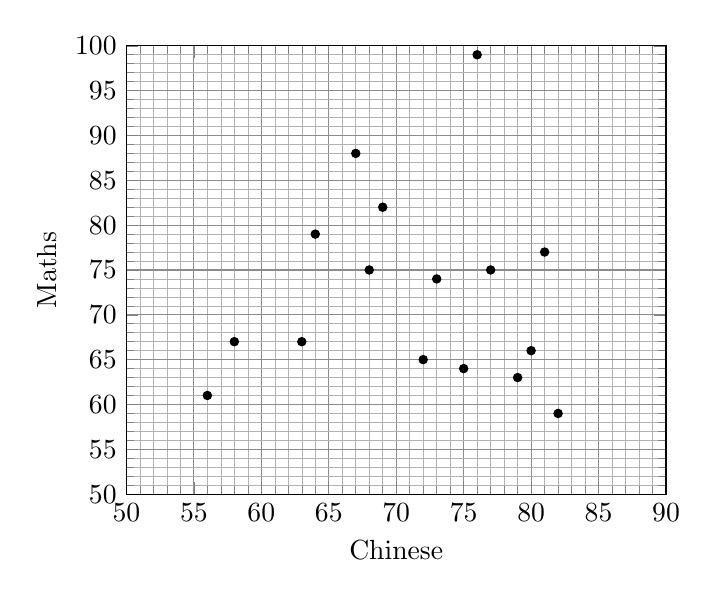
\begin{tikzpicture}
                        \begin{axis}[
                            xlabel=Chinese,
                            ylabel=Maths,
                            xmin=50, xmax=90,
                            ymin=50, ymax=100,
                            xtick={50, 55, ..., 90},
                            ytick={50, 55, ..., 100},
                            grid=both,
                            grid style={line width=.2pt, draw=gray!60},
                            major grid style={line width=.4pt,draw=gray!90},
                            minor tick num=4,
                          ]
                          \addplot[mark=*, mark size=1.5, mark options={solid, fill=black}, only marks] coordinates {(82,59) (79,63) (76,99) (63,67) (56,61) (67,88) (69,82) (81,77) (77,75) (73,74) (58,67) (64,79) (68,75) (72,65) (75,64) (80,66)};
                        \end{axis}
                      \end{tikzpicture}
                    }
                  \end{center}
            \item Find the correlation coefficient of the two exams, and determine the strength
                  of correlation. \sol{}
                  \begin{center}
                    \begin{tabular}{|c|c|c|c|c|}
                      \hline
                      $x_i$       & $y_i$       & $x_i^2$       & $y_i^2$       & $x_iy_i$       \\
                      \hline
                      82          & 59          & 6724          & 3481          & 4838           \\
                      79          & 63          & 6241          & 3969          & 4977           \\
                      76          & 99          & 5776          & 9801          & 7524           \\
                      63          & 67          & 3969          & 4489          & 4221           \\
                      56          & 61          & 3136          & 3721          & 3416           \\
                      67          & 88          & 4489          & 7744          & 5896           \\
                      69          & 82          & 4761          & 6724          & 5658           \\
                      81          & 77          & 6561          & 5929          & 6237           \\
                      77          & 75          & 5929          & 5625          & 5775           \\
                      73          & 74          & 5329          & 5476          & 5402           \\
                      58          & 67          & 3364          & 4489          & 3886           \\
                      64          & 79          & 4096          & 6241          & 5056           \\
                      68          & 75          & 4624          & 5625          & 5100           \\
                      72          & 65          & 5184          & 4225          & 4680           \\
                      75          & 64          & 5625          & 4096          & 4800           \\
                      80          & 66          & 6400          & 4356          & 5280           \\
                      \hline
                      \hline
                      $\sum{x_i}$ & $\sum{y_i}$ & $\sum{x_i^2}$ & $\sum{y_i^2}$ & $\sum{x_iy_i}$ \\
                      \hline
                      1140        & 1161        & 82208         & 85991         & 82746          \\
                      \hline
                    \end{tabular}
                  \end{center}
                  \begin{flalign*}
                    \bar{x}                                                   & = \frac{1140}{16} = 71.25                                                  \\
                    \bar{y}                                                   & = \frac{1161}{16} = 72.56                                                  \\
                    r                                                         & = \frac{\frac{82746}{16} - 71.25 \cdot 72.56}{\sqrt{\left(\frac{82208}{16}
                    - 71.25^2\right)\left(\frac{85991}{16} - 72.56^2\right)}} &                                                                            \\
                                                                              & = 0.0189
                  \end{flalign*}

                  According to the result of the calculation, the marks of Chinese exam and Maths
                  exam of the 16 senior students are positively and weakly correlated.
          \end{enumerate}

    \item The table below shows the prices of a product (in \$) in 2005, 2010, and 2015:
          \begin{center}
            \begin{tabular}{|c|c|c|c|}
              \hline
              Year  & 2005 & 2010 & 2015 \\
              \hline
              Price & 4    & 6    & $x$  \\
              \hline
            \end{tabular}
          \end{center}
          \begin{enumerate}
            \item Assume that the percentage of price increase from 2005 to 2010 is the same as
                  that from 2010 to 2015, find the value of $x$. \sol{}
                  \begin{flalign*}
                    \frac{6}{4} \cdot 100\% & = \frac{x}{6} \cdot 100\% \\
                    \frac{6}{4}             & = \frac{x}{6}             \\
                    4x                      & = 36                      \\
                    x                       & = 9
                  \end{flalign*}
            \item Find the relative price in 2015 with respect to 2005. \sol{}
                  \begin{flalign*}
                    P.R. & = \frac{9}{4} \cdot 100\% = 225\%
                  \end{flalign*}
          \end{enumerate}

    \item The price data of primary food of a city with 2013 as base period and 2014 as
          current period are as follows:
          \begin{center}
            \begin{tabular}{|c|c|c|}
              \hline
              Food                   & Relative price & Weight \\
              \hline
              Meat                   & 105            & 8      \\
              Fish                   & 111            & 7      \\
              Vegetables             & 98             & 5      \\
              Rice        \& Noodles & 103            & 10     \\
              Cooking Oil            & 100            & 3      \\
              Beverage               & 107            & 2      \\
              Fruits                 & 99             & 2      \\
              \hline
            \end{tabular}
          \end{center}
          Find the price index in 2014.
          \sol{}
          \begin{flalign*}
            \text{Price Index} & = \frac{105 \cdot 8 + 111 \cdot 7 + \cdots + 99 \cdot 2}{37} \\
                               & = \frac{3849}{37}                                            \\
                               & = 104.03
          \end{flalign*}

    \item The relative price of daily expenses of people in a place with repsect to last
          year and their relative consumption are as follows:
          \begin{center}
            \resizebox{\columnwidth - 4.6em}{!}{
              \begin{tabular}{|c|c|c|}
                \hline
                Daily Expenses & Relative price & Relative Consumption \\
                \hline
                Clothing       & 120            & 23                   \\
                Food           & 117            & 40                   \\
                Housing        & 132            & 19                   \\
                Transportation & 130            & 18                   \\
                \hline
              \end{tabular}
            }
          \end{center}
          Using the relative consumption as weight, find the composite index of daily expenses.
          \sol{}
          \begin{flalign*}
            \text{Composite Index} & = \frac{120 \cdot 23 + \cdots + 130 \cdot 18}{100} \\
                                   & = \frac{12288}{100}                                \\
                                   & = 122.88
          \end{flalign*}

    \item The table below shows the spending of a company in 4 different projects in 3
          consecutive years:
          \begin{center}
            \resizebox{\columnwidth - 4.6em}{!}{
              \begin{tabular}{|c|c|c|c|c|c|}
                \hline
                \multirow{2}{*}{Project} & \multicolumn{3}{c|}{Year} & \multirow{2}{*}{A} & \multirow{2}{*}{B}             \\
                \cline{2-4}
                                         & 2012                      & 2013               & 2014               &     &     \\
                \hline
                Salaries                 & $x$                       & 20,000             & 30,000             & 150 & $P$ \\
                Stationery               & 5,000                     & $y$                & 7,000              & 120 & 140 \\
                Repair                   & 4,000                     & 5000               & $z$                & 125 & 150 \\
                Miscellaneous            & 8,000                     & $Q$                & 15,000             & $R$ & $R$ \\
                \hline
              \end{tabular}
            }
          \end{center}
          Given that $A$ is the index where 2012 is the base period and 2013 is the current period; $B$ is the index where 2012 is the base period and 2014 is the current period. Find the value of $x$, $y$, $z$, $P$, $Q$, and $R$.
          \sol{}
          \begin{flalign*}
            \frac{20000}{x} \cdot 100 & = 150      \\
            \frac{20000}{x}           & = 1.5      \\
            1.5x                      & = 20000    \\
            x                         & = 13333.33 \\
          \end{flalign*}
          \begin{flalign*}
            P & = \frac{30000}{13333.33} \cdot 100 \\
              & = 225
          \end{flalign*}
          \begin{flalign*}
            \frac{y}{5000} \cdot 100 & = 120  \\
            \frac{y}{5000}           & = 1.2  \\
            y                        & = 6000
          \end{flalign*}
          \begin{flalign*}
            \frac{z}{4000} \cdot 100 & = 150  \\
            \frac{z}{4000}           & = 1.5  \\
            z                        & = 6000
          \end{flalign*}
          \begin{flalign*}
            \frac{Q}{8000} \cdot 100 & = \frac{15000}{8000} \cdot 100 = R \\
            \frac{Q}{8000}           & = 1.875 = \frac{R}{100}            \\
            Q                        & = 15000                            \\
            R                        & = 187.5
          \end{flalign*}
          \begin{flalign*}
            \therefore\ x & = 13333.33,\ y = 6000,\ z = 6000, \\
            P             & = 225,\ Q = 15000,\ R = 187.5
          \end{flalign*}
  \end{enumerate}

  \chapter{Permutations and Combinations}

  Permutations and combinations are the foundation of probability and statistics.
  In our daily life, we often need to calculate the number of ways of completing
  a task. These calculations are based on two basic principles: addition
  principle and multiplication principle.

  \section{Addition and Multiplication Principles}

  \begin{theorem}{Addition Principle}

    If there are $n$ methods of doing a task, the first method can be done in $m_1$
    ways, the second method can be done in $m_2$ ways, $\cdots$, the $n$th methods
    can be done in $m_n$ ways, and they are mutually exclusive, which means he task
    can be done in whatever way using whatever method, then the total number of
    ways of doing the task is
    \begin{cequation}
      m_1 + m_2 + \cdots + m_n
    \end{cequation}
  \end{theorem}

  \begin{theorem}{Multiplication Principle}

    If there are $n$ steps in doing a task, the first step can be done in $m_1$
    ways, the second step can be done in $m_2$ ways, $\cdots$, the $n$th steps can
    be done in $m_n$ ways, then the total number of ways of doing the task is
    \begin{cequation}
      m_1 \cdot m_2 \cdot \cdots \cdot m_n
    \end{cequation}
  \end{theorem}

  \subsection{Practice 1}
  \begin{enumerate}
    \item There are 2 Math reference books, 3 novels, and 4 storybooks of idioms. Xiao
          Hua wants to choose one book from each category. How many ways can he choose?
          \sol{}

          To choose one book from each category, there are 3 steps:
          \begin{itemize}
            \item First step, choose a Math reference book, which can be done in 2 ways.
            \item Second step, choose a novel, which can be done in 3 ways.
            \item Third step, choose a storybook of idioms, which can be done in 4 ways.
          \end{itemize}
          All these steps must be done in order to complete the task. Therefore, applying the multiplication principle, there are $2 \cdot 3 \cdot 4 = 24$ ways to choose one book from each category.

    \item Travelling from $A$ to $B$ can be done by bus or train. There are 4 buses and 3
          trains. How many ways are there to travel from $A$ to $B$? \sol{}

          To travel from $A$ to $B$, there are 2 method:
          \begin{itemize}
            \item First method, travel by bus, which can be done in 4 ways.
            \item Second method, travel by train, which can be done in 3 ways.
          \end{itemize}
          Any way in any method can be used to travel from $A$ to $B$. Therefore, applying the addition principle, there are $4 + 3 = 7$ ways to travel from $A$ to $B$.
  \end{enumerate}

  \subsection{Practice 19.1}
  \begin{enumerate}
    \item During the eve of a festival, there are 3 trains, 4 buses, and 4 trains from
          Johor Bahru to Pinang. How many ways are there to travel from Johor Bahru to
          Pinang during the day? \sol{}

          To travel from Johor Bahru to Pinang, there are 3 methods:
          \begin{itemize}
            \item First method, travel by train, which can be done in 3 ways.
            \item Second method, travel by bus, which can be done in 4 ways.
            \item Third method, travel by train, which can be done in 4 ways.
          \end{itemize}
          Any way in any method can be used to travel from Johor Bahru to Pinang. Therefore, applying the addition principle, there are $3 + 4 + 4 = 11$ ways to travel from Johor Bahru to Pinang.

    \item One has 13 shirts and 6 pants, how many ways can he dress up? \sol{}

          To dress up, there are 2 steps:
          \begin{itemize}
            \item First step, choose a shirt, which can be done in 13 ways.
            \item Second step, choose a pants, which can be done in 6 ways.
          \end{itemize}
          All these steps must be done in order to complete the task. Therefore, applying the multiplication principle, there are $13 \cdot 6 = 78$ ways to dress up.

    \item There are 4 airlines $A$, $B$, $C$, and $D$ that provide flights from Kuala
          Lumpur to Bangkok: $A$ provdies 3 flights per day, $B$ provides 2 flights per
          day, $C$ and $D$ provides 1 flight per day. How many choices are there to
          travel from Kuala Lumpur to Bangkok? \sol{}

          To travel from Kuala Lumpur to Bangkok, there are 4 methods:
          \begin{itemize}
            \item First method, travel by $A$, which can be done in 3 ways.
            \item Second method, travel by $B$, which can be done in 2 ways.
            \item Third method, travel by $C$, which can be done in 1 way.
            \item Fourth method, travel by $D$, which can be done in 1 way.
          \end{itemize}
          Any way in any method can be used to travel from Kuala Lumpur to Bangkok. Therefore, applying the addition principle, there are $3 + 2 + 1 + 1 = 7$ ways to travel from Kuala Lumpur to Bangkok.

    \item How many set meal combinations are there if there are 6 type of main dishes, 5
          type of drinks, and 2 type of desserts? \sol{}

          To make a set meal, there are 3 steps:
          \begin{itemize}
            \item First step, choose a main dish, which can be done in 6 ways.
            \item Second step, choose a drink, which can be done in 5 ways.
            \item Third step, choose a dessert, which can be done in 2 ways.
          \end{itemize}
          All these steps must be done in order to complete the task. Therefore, applying the multiplication principle, there are $6 \cdot 5 \cdot 2 = 60$ ways to make a set meal.

    \item There are 4 doors in a classroom, student $A$ and student $B$ can enter the
          classroom through any door. How many ways are there for student $A$ and student
          $B$ to enter the classroom? \sol{}

          To enter the classroom, there are 2 steps:
          \begin{itemize}
            \item First step, student $A$ choose a door, which can be done in 4 ways.
            \item Second step, student $B$ choose a door, which can be done in 4 ways.
          \end{itemize}
          All these steps must be done in order to complete the task. Therefore, applying the multiplication principle, there are $4 \cdot 4 = 16$ ways for student $A$ and student $B$ to enter the classroom.

    \item A friendly match is held between 2 ping pong teams, each team has to send 3
          players, and each player has to play games with all the other players on the
          other team. How many games have to be played? \sol{}

          To play a game betwen two teams: $A$ and $B$, there are 3 steps:
          \begin{itemize}
            \item First step, choose a player from the team $A$, which can be done in 3 ways.
            \item Second step, choose a player from team $B$, which can be done in 3 ways.
          \end{itemize}
          To match between all players from team $A$ and team $B$, there are $3 \cdot 3 = 9$ games have to be played.

    \item Matching 8 clothes of different colors with 5 different skirts, how many ways
          are there to dress up? If the above dresses are paired with 4 pairs of shoes of
          different colors, how many ways are there to dress up? \sol{}

          To dress up, there are 2 steps:
          \begin{itemize}
            \item First step, choose a clothes, which can be done in 8 ways.
            \item Second step, choose a skirt, which can be done in 5 ways.
          \end{itemize}
          All these steps must be done in order to complete the task. Therefore, applying the multiplication principle, there are $8 \cdot 5 = 40$ combinations of clothes and skirts.

          To pair the clothes and skirts with shoes, there are 2 steps:
          \begin{itemize}
            \item First step, choose a clothes and a skirt, which can be done in 40 ways.
            \item Second step, choose a shoes, which can be done in 4 ways.
          \end{itemize}
          All these steps must be done in order to complete the task. Therefore, applying the multiplication principle, there are $40 \cdot 4 = 160$ combinations of clothes, skirts, and shoes.

  \end{enumerate}

  \section{Permutations and Permutation Formula}

  \subsection{Practice 2}

  How many ways are there to arrange the numbers 1, 2, 3, 4 into a two digit
  number with no repeated digits? \sol{}

  First step: choose one of the 4 numbers as the first digit, there are 4 ways to
  do so.

  Second step: choose one of the remaining 3 numbers as the second digit, there
  are 3 ways to do so.

  According to the multiplication principle, the total number of ways to arrange
  the numbers 1, 2, 3, 4 into a two digit number with no repeated digits is $4
    \cdot 3 = 12$. \\\\ If there are $n$ elements, we want to pick $r$ elements
  from them and arrange them in a sequence, how many ways are there to do so?
  This question can be treated as there are $r$ empty boxes, which means this
  requires $r$ steps to complete.

  \begin{center}
    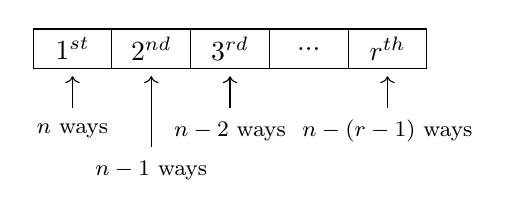
\begin{tikzpicture}
      \draw (0,0) -- (0,0.5) -- (5,0.5) -- (5,0) -- (0,0);
      \draw (1, 0) -- (1, 0.5);
      \draw (2, 0) -- (2, 0.5);
      \draw (3, 0) -- (3, 0.5);
      \draw (4, 0) -- (4, 0.5);
      \node at (0.5, 0.25) {$1^{st}$};
      \node at (1.5, 0.25) {$2^{nd}$};
      \node at (2.5, 0.25) {$3^{rd}$};
      \node at (3.5, 0.25) {$...$};
      \node at (4.5, 0.25) {$r^{th}$};
      \draw [->] (0.5, -0.5) -- (0.5, -0.1);
      \draw [->] (1.5, -1.0) -- (1.5, -0.1);
      \draw [->] (2.5, -0.5) -- (2.5, -0.1);
      \draw [->] (4.5, -0.5) -- (4.5, -0.1);
      \node at (0.5, -0.8) {\footnotesize{$n$ ways}};
      \node at (1.5, -1.3) {\footnotesize{$n-1$ ways}};
      \node at (2.5, -0.8) {\footnotesize{$n-2$ ways}};
      \node at (4.5, -0.8) {\footnotesize{$n-(r-1)$ ways}};
    \end{tikzpicture}
  \end{center}

  First step: Choose one element from $n$ elements and put it in the first box,
  then there are $n$ ways to do so.

  Second step: Choose one element from $n-1$ elements and put it in the second
  box, then there are $n-1$ ways to do so.

  Third step: Choose one element from $n-2$ elements and put it in the third box,
  then there are $n-2$ ways to do so.

  So on and so forth, when $r-1$ boxes are filled, the last box $r$ can only be
  filled with one of the remaining $n-(r-1)$ elements, so there are $n-(r-1)$
  ways to do so. According to the multiplication principle, the total number of
  ways to fill in $r$ boxes is
  \begin{cequation}
    n(n-1)(n-2) \cdots (n-r+1)
  \end{cequation}
  Threrefore, there are $n(n-1)(n-2) \cdots (n-r+1)$ ways to arrange $r$ elements, and this denoted as $\permtwo[n]{r}$, $\permtwo[n]{r}$, or $P^n_r$.
  \begin{cequation}
    \permtwo[n]{r} = n(n-1)(n-2) \cdots (n-r+1)
  \end{cequation}
  Where $r \leq n$, $n \in N$, $r = 0, 1, 2, \cdots, n$. This formula is called
  the permutation formula.

  When $r = n$, aka a full permutation, the formula becomes
  \begin{cequation}
    \permtwo[n]{n} = n(n-1)(n-2) \cdots 3 \cdot 2 \cdot 1
  \end{cequation}
  Therefore, the permutation of all $n$ elements is equal to the products of natural numbers from 1 to $n$. This is called the factorial of $n$, denoted as $n!$.
  \makeatletter
  \setbool{@fleqn}{false}
  \makeatother
  \begin{flalign*}
    n! & = \permtwo[n]{n}                       \\
       & = n(n-1)(n-2) \cdots 3 \cdot 2 \cdot 1
  \end{flalign*}
  \makeatletter
  \setbool{@fleqn}{true}
  \makeatother

  Using factorial, the permutation formula can be transform into the following:
  \begin{flalign*}
    \permtwo[n]{r} & = n(n-1)(n-2) \cdots (n-r+1)                                                                      \\
                   & = \frac{n(n-1)(n-2) \cdots (n-r+1)(n-r) \cdots 3 \cdot 2 \cdot 1}{(n-r) \cdots 3 \cdot 2 \cdot 1} \\
                   & = \frac{n!}{(n-r)!}
  \end{flalign*}

  Hence, the permutation formula can be written as
  \begin{cequation}
    \permtwo[n]{r} = \frac{n!}{(n-r)!}
  \end{cequation}

  Note: $0!$ is defined as 1 to make the formula work when $n = r$.

  \subsection{Practice 3}

  \begin{enumerate}
    \item Find the value of $\permtwo[7]{3}$ and $5!$. \sol{}
          \begin{flalign*}
            \permtwo[7]{3} & = 7 \cdot 6 \cdot 5                 \\
                           & = 210                               \\
            5!             & = 5 \cdot 4 \cdot 3 \cdot 2 \cdot 1 \\
                           & = 120
          \end{flalign*}

    \item Calculate $\permtwo[10]{3} + \permtwo[8]{4}$. \sol{}
          \begin{flalign*}
            \permtwo[10]{3} + \permtwo[8]{4} & = 10 \cdot 9 \cdot 8 + 8 \cdot 7 \cdot 6 \cdot 5 \\
                                             & = 720 + 1680                                     \\
                                             & = 2400
          \end{flalign*}
    \item If $100(\permtwo[n]{2}) = \permtwo[2n]{3}$, find the value of $n$. \sol{}
          \setlength{\belowdisplayskip}{0pt} \setlength{\belowdisplayshortskip}{0pt}
          \setlength{\abovedisplayskip}{0pt} \setlength{\abovedisplayshortskip}{0pt}
          \begin{flalign*}
            100(\permtwo[n]{2}) & = \permtwo[2n]{3}  & \\
            100(n)(n-1)         & = (2n)(2n-1)(2n-2)   \\
            100(n)(n-1)         & = 4(n)(2n-1)(n-1)
          \end{flalign*}
          \begin{flalign*}
            100(n)(n-1) - 4(n)(2n-1)(n-1)                     & = 0  \\
            4(n)(n-1)[25 - (2n-1)]                            & = 0  \\
            (n)(n-1)(25 - 2n + 1)                             & = 0  \\
            (n)(n-1)(26 - 2n)                                 & = 0  \\
            -2(n)(n-1)(n - 13)                                & = 0  \\
            (n)(n-1)(n - 13)                                  & = 0  \\
            \therefore\ n = 0 \text{ or } n = 1 \text{ or } n & = 13
          \end{flalign*}
          \begin{flalign*}
            \because\ n   & \in \mathbb{N},\ n \geq 3 \\
            \therefore\ n & = 13
          \end{flalign*}
          \setlength{\belowdisplayskip}{\baselineskip} \setlength{\belowdisplayshortskip}{\baselineskip}
          \setlength{\abovedisplayskip}{\baselineskip} \setlength{\abovedisplayshortskip}{\baselineskip}
  \end{enumerate}

  \subsection{Exercise 19.2a}

  \begin{enumerate}
    \item Write down all the permutations of 3 elements in 4 elements $A$, $B$, $C$, $D$.
          \sol{}

          $ABC$, $ABD$, $ACB$, $ACD$, $ADB$, $ADC$, $BAC$, $BAD$, $BCA$, $BCD$, $BDA$, $BDC$, $CAB$, $CAD$, $CBA$, $CBD$, $CDA$, $CDB$, $DAB$, $DAC$, $DBA$, $DBC$, $DCA$, $DCB$

    \item Calculate:
          \begin{enumerate}
            \item $\permtwo[15]{4}$
                  \sol{}
                  \begin{flalign*}
                    \permtwo[15]{4} & = 15 \cdot 14 \cdot 13 \cdot 12 \\
                                    & = 32760
                  \end{flalign*}

            \item $\permtwo[100]{3}$
                  \sol{}
                  \begin{flalign*}
                    \permtwo[100]{3} & = 100 \cdot 99 \cdot 98 \\
                                     & = 970200
                  \end{flalign*}

            \item $7!$
                  \sol{}
                  \begin{flalign*}
                    7! & = 7 \cdot 6 \cdot 5 \cdot 4 \cdot 3 \cdot 2 \cdot 1 \\
                       & = 5040
                  \end{flalign*}

            \item $\frac{8!}{5!}$
                  \sol{}
                  \begin{flalign*}
                    \frac{8!}{5!} & = \frac{8!}{(8-3)!} \\
                                  & = \permtwo[8]{3}    \\
                                  & = 8 \cdot 7 \cdot 6 \\
                                  & = 336
                  \end{flalign*}
          \end{enumerate}

    \item Calculate the following:
          \begin{enumerate}
            \item $\frac{11! - 10!}{10! - 9!}$
                  \sol{}
                  \begin{flalign*}
                    \frac{11! - 10!}{10! - 9!} & = \frac{11 \cdot 10! - 10!}{10 \cdot 9! - 9!} \\
                                               & = \frac{10! \cdot 10}{9! \cdot 9}             \\
                                               & = \frac{10 \cdot 10 \cdot 9!}{9! \cdot 9}     \\
                                               & = \frac{10 \cdot 10}{9}                       \\
                                               & = \frac{100}{9}
                  \end{flalign*}

            \item $\frac{7! - 6! - 5!}{5!}$
                  \sol{}
                  \begin{flalign*}
                    \frac{7! - 6! - 5!}{5!} & = \frac{7 \cdot 6 \cdot 5! - 6 \cdot 5! - 5!}{5!} \\
                                            & = \frac{5!(7 \cdot 6 - 6 - 1)}{5!}                \\
                                            & = 42 - 7                                          \\
                                            & = 35
                  \end{flalign*}

            \item $\frac{13! - 12!}{{(12)}^2 10!}$
                  \sol{}
                  \begin{flalign*}
                    \frac{13! - 12!}{{(12)}^2 10!} & = \frac{13 \cdot 12! - 12!}{(12)^2 10!}      \\
                                                   & = \frac{12!(12)}{(12)^2 10!}                 \\
                                                   & = \frac{12!}{12 \cdot 10!}                   \\
                                                   & = \frac{12 \cdot 11 \cdot 10!}{12 \cdot 10!} \\
                                                   & = 11
                  \end{flalign*}

            \item $\frac{5(\permtwo[8]{3})}{2(\permtwo[6]{2})}$
                  \sol{}
                  \begin{flalign*}
                    \frac{5(\permtwo[8]{3})}{2(\permtwo[6]{2})} & = \frac{5 \cdot (8 \cdot 7 \cdot 6)}{2 \cdot (6 \cdot 5)} \\
                                                                & = \frac{1680}{60}                                         \\
                                                                & = 28
                  \end{flalign*}

            \item $\frac{\permtwo[9]{5} + \permtwo[9]{4}}{\permtwo[9]{3}}$
                  \sol{}
                  \begin{flalign*}
                    \frac{\permtwo[9]{5} + \permtwo[9]{4}}{\permtwo[9]{3}} & = \frac{\frac{9!}{(9-5)!} + \frac{9!}{(9-4)!}}{\frac{9!}{(9-3)!}} \\
                                                                           & = \frac{\frac{9!}{4!} + \frac{9!}{5!}}{\frac{9!}{6!}}             \\
                                                                           & = \frac{9!(4! + 5!)}{4!5!} \cdot \frac{6!}{9!}                    \\
                                                                           & = \frac{6!(4! + 5!)}{4!5!}                                        \\
                                                                           & = \frac{6 \cdot 5 \cdot 4!(4! + 5!)}{4!5!}                        \\
                                                                           & = \frac{6 \cdot 5(4! + 5!)}{5!}                                   \\
                                                                           & = \frac{6 \cdot 5(4! + 5!)}{5 \cdot 4!}                           \\
                                                                           & = \frac{6(4! + 5!)}{4!}                                           \\
                                                                           & = \frac{3!(4! + 5!)}{4 \cdot 3!}                                  \\
                                                                           & = \frac{4! + 5!}{4}                                               \\
                                                                           & = \frac{4 \cdot 3! + 5 \cdot 4 \cdot 3!}{4}                       \\
                                                                           & = \frac{4 \cdot 3! \cdot 6}{4}                                    \\
                                                                           & = 6 \cdot 3!                                                      \\
                                                                           & = 6 \cdot 6                                                       \\
                                                                           & = 36
                  \end{flalign*}
            \item $\frac{\permtwo[12]{12} - \permtwo[11]{11}}{\permtwo[10]{10}}$
                  \sol{}
                  \begin{flalign*}
                    \frac{\permtwo[12]{12} - \permtwo[11]{11}}{\permtwo[10]{10}} & = \frac{12! - 11!}{10!}             \\
                                                                                 & = \frac{12 \cdot 11! - 11!}{10!}    \\
                                                                                 & = \frac{11 \cdot 11!}{10!}          \\
                                                                                 & = \frac{11 \cdot 11 \cdot 10!}{10!} \\
                                                                                 & = 11 \cdot 11                       \\
                                                                                 & = 121
                  \end{flalign*}
          \end{enumerate}

    \item Simplify the following:
          \begin{enumerate}
            \item $\frac{(n+1)!}{(n-1)!}$
                  \sol{}
                  \begin{flalign*}
                    \frac{(n+1)!}{(n-1)!} & = \frac{(n+1)n(n-1)!}{(n-1)!} \\
                                          & = n(n+1)
                  \end{flalign*}

            \item $\frac{(20 - r)!}{(18 - r)!}$
                  \sol{}
                  \begin{flalign*}
                    \frac{(20 - r)!}{(18 - r)!} & = \frac{(20 - r)(19 - r)(18 - r)!}{(18 - r)!} \\
                                                & = (20 - r)(19 - r)
                  \end{flalign*}
          \end{enumerate}

    \item Find the value of $n$ or $r$ of the following expressions:
          \begin{enumerate}
            \item $\frac{(n+1)!}{n!} = 42$
                  \sol{}
                  \begin{flalign*}
                    \frac{(n+1)!}{n!}  & = 42  \\
                    \frac{(n+1)n!}{n!} & =  42 \\
                    n+1                & = 42  \\
                    n                  & = 41
                  \end{flalign*}

            \item $127(\permtwo[2n]{3}) = \permtwo[2n]{4}$
                  \sol{}
                  \begin{flalign*}
                    127(\permtwo[2n]{3})                              & = \permtwo[2n]{4} \\
                    \frac{\permtwo[2n]{4}}{\permtwo[2n]{3}}           & = 127             \\
                    \frac{(2n)!}{(2n-4)!} \cdot \frac{(2n-3)!}{(2n)!} & = 127             \\
                    \frac{(2n-3)!}{(2n-4)!}                           & = 127             \\
                    \frac{(2n-3)(2n-4)!}{(2n-4)!}                     & = 127             \\
                    2n-3                                              & = 127             \\
                    2n                                                & = 130             \\
                    n                                                 & = 65
                  \end{flalign*}

            \item $18(\permtwo[n-1]{2}) = \permtwo[n]{4}$
                  \sol{}
                  \setlength{\belowdisplayskip}{0pt} \setlength{\belowdisplayshortskip}{0pt}
                  \setlength{\abovedisplayskip}{0pt} \setlength{\abovedisplayshortskip}{0pt}
                  \begin{flalign*}
                    18(\permtwo[n-1]{2})                                   & = \permtwo[n]{4} \\
                    \frac{\permtwo[n]{4}}{\permtwo[n-1]{2}}                & = 18             \\
                    \frac{n!}{(n-4)!} \cdot \frac{(n-3)!}{(n-1)!}          & = 18             \\
                    \frac{n(n-1)!}{(n-4)!} \cdot \frac{(n-3)!}{(n-1)!}     & = 18             \\
                    \frac{n(n-3)!}{(n-4)!}                                 & = 18             \\
                    \frac{n(n-3)(n-4)!}{(n-4)!}                            & = 18             \\
                    n(n-3)                                                 & = 18             \\
                    n^2 - 3n                                           -18 & = 0              \\
                    (n-6)(n+3)                                             & = 0              \\
                    n = 6 \text{ or } n                                    & -3
                  \end{flalign*}
                  \begin{flalign*}
                    \because\    & n \in \mathbb{N},\ n \geq 4 \\
                    \therefore\  & n = 6
                  \end{flalign*}
                  \setlength{\belowdisplayskip}{\baselineskip} \setlength{\belowdisplayshortskip}{\baselineskip}
                  \setlength{\abovedisplayskip}{\baselineskip} \setlength{\abovedisplayshortskip}{\baselineskip}

            \item $\permtwo[2n+1]{4} = 132(\permtwo[n]{3})$
                  \sol{}
                  \setlength{\belowdisplayskip}{0pt} \setlength{\belowdisplayshortskip}{0pt}
                  \setlength{\abovedisplayskip}{0pt} \setlength{\abovedisplayshortskip}{0pt}
                  \begin{flalign*}
                    \permtwo[2n+1]{4}                               & = 132(\permtwo[n]{3}) & \\
                    \frac{\permtwo[2n+1]{4}}{\permtwo[n]{3}}        & = 132                   \\
                    \frac{(2n+1)!}{(2n-3)!} \cdot \frac{(n-3)!}{n!} & = 132                   \\
                    \resizebox{\columnwidth - 10em}{!}{
                      $\frac{(2n+1)(2n)(2n-1)(2n-2)(2n-3)!}{(2n-3)!} \cdot \frac{(n-3)!}{n(n-1)(n-2)(n-3)!}$
                    }                                               & = 132                   \\
                    \frac{(2n+1)(2n)(2n-1)(2n-2)}{n(n-1)(n-2)}      & = 132                   \\
                    \frac{4n(n-1)(2n+1)(2n-1)}{n(n-1)(n-2)}         & = 132                   \\
                    \frac{(2n+1)(2n-1)}{n-2}                        & = 33                    \\
                    4n^2 - 1                                        & = 33n - 66              \\
                    4n^2 - 33n + 65                                 & = 0                     \\
                    (n-5)(4n-13)                                    & = 0                     \\
                    n = 5 \text{ or } n                             & = \frac{13}{4}
                  \end{flalign*}
                  \begin{flalign*}
                    \because\    & n \in \mathbb{N},\ n \geq 3 \\
                    \therefore\  & n = 5
                  \end{flalign*}
                  \setlength{\belowdisplayskip}{\baselineskip} \setlength{\belowdisplayshortskip}{\baselineskip}
                  \setlength{\abovedisplayskip}{\baselineskip} \setlength{\abovedisplayshortskip}{\baselineskip}

            \item $4(\permtwo[10]{r-1}) = \permtwo[10]{r}$
                  \sol{}
                  \begin{flalign*}
                    4(\permtwo[10]{r-1})                            & = \permtwo[10]{r} \\
                    \frac{\permtwo[10]{r}}{\permtwo[10]{r-1}}       & = 4               \\
                    \frac{10!}{(10-r)!} \cdot \frac{(10-r+1)!}{10!} & = 4               \\
                    \frac{(10-r+1)!}{(10-r)!}                       & = 4               \\
                    \frac{(10-r+1)(10-r)!}{(10-r)!}                 & = 4               \\
                    10-r+1                                          & = 4               \\
                    11-r                                            & = 4               \\
                    r                                               & = 7
                  \end{flalign*}

            \item $6(\permtwo[9]{r-2}) = \permtwo[9]{r}$
                  \sol{}
                  \setlength{\belowdisplayskip}{0pt} \setlength{\belowdisplayshortskip}{0pt}
                  \setlength{\abovedisplayskip}{0pt} \setlength{\abovedisplayshortskip}{0pt}
                  \begin{flalign*}
                    6(\permtwo[9]{r-2})                         & = \permtwo[9]{r} \\
                    \frac{\permtwo[9]{r}}{\permtwo[9]{r-2}}     & = 6              \\
                    \frac{9!}{(9-r)!} \cdot \frac{(9-r+2)!}{9!} & = 6              \\
                    \frac{(9-r+2)!}{(9-r)!}                     & = 6              \\
                    \frac{(9-r+2)(9-r+1)(9-r)!}{(9-r)!}         & = 6              \\
                    (9-r+2)(9-r+1)                              & = 6              \\
                    (11-r)(10-r)                                & = 6              \\
                    r^2 - 21r + 110                             & = 6              \\
                    r^2 - 21r + 104                             & = 0              \\
                    (r-13)(r-8)                                 & = 0              \\
                    r = 13 \text{ or } r                        & = 8
                  \end{flalign*}
                  \begin{flalign*}
                    \because\    & r \in \mathbb{N},\ r \leq 11 \\
                    \therefore\  & r = 8
                  \end{flalign*}
                  \setlength{\belowdisplayskip}{\baselineskip} \setlength{\belowdisplayshortskip}{\baselineskip}
                  \setlength{\abovedisplayskip}{\baselineskip} \setlength{\abovedisplayshortskip}{\baselineskip}
          \end{enumerate}
  \end{enumerate}

  \subsection{Practice 4}
  \begin{enumerate}
    \item How many 3 digit numbers with no repeated digits can be formed using the digits
          1, 2, 3, 4, 5? \sol{}

          There are $\permtwo[5]{3} = 5 \cdot 4 \cdot 3 = 60$ ways to form a 3 digit
          number with these 5 digits.

    \item How many 3 digit numbers with no repeated digits can be formed using the digits
          0, 1, 2, 3, 4? \sol{}

          Since the hundred's digit cannot be 0, there are 4 digits to choose from.
          Therefore, there are $4 \cdot \permtwo[4]{2} = 4 \cdot 4 \cdot 3 = 48$ ways to
          form a 3 digit number with these 5 digits.
  \end{enumerate}

  \subsection{Practice 5}
  \begin{enumerate}
    \item There are 50 seats and 50 students in a class. How many ways can the students
          be seated in the class? \sol{}

          There are $\permtwo[50]{50} = 50!$ ways to seat the students.

    \item Person $A$ and $B$ has two choose two adjacent seats in a row of 5 chairs. How
          many ways can they be seated? \sol{}

          There are 4 ways to seat one person in one chair and the other person in the
          chair at the right of the first person. There are $2!$ ways to arrange person
          $A$ and $B$ in these two chairs, so there are $4 \cdot 2 = 8$ ways to seat the
          two persons.

    \item 4 boys and 2 girls are standing in a row to take a photo. Assume that the two girls has to stand next to each other, how many ways can they be arranged?
          \sol{}

          Treat these two girls as one, there are $5!$ ways to arrange the 5 persons. The
          two girls can switch places, so there are $2!$ ways to arrange them. Therefore,
          there are $5! \cdot 2! = 240$ ways to arrange the 6 persons.
  \end{enumerate}

  \subsection{Exercise 19.2b}

  \begin{enumerate}
    \item Assume that there is no repeated digits, how many 5 digit numbers can be formed
          using the digits 1, 2, 3, 4, 5? \sol{}

          There are $\permtwo[5]{5} = 5! = 120$ ways to form a 5 digit number with these
          5 digits.

    \item How many ways are there to arrange the flags of 10 ASEAN members in a row?
          \sol{}

          There are $\permtwo[10]{10} = 10! = 3628800$ ways to arrange the flags of the
          10 ASEAN members in a row.

    \item 7 novel stories are to be compiled into a book. The sortest story must be placed
          at the beginning of the book, while the longest story must be placed at the end. How many ways can the stories be arranged?
          \sol{}

          Since the first book and the last book are fixed, there are $\permtwo[5]{5} =
            5! = 120$ ways to arrange the 5 books in the middle.

    \item Ten students are to be arranged in a row. Two of the tallest students must be
          placed at the beginning of the row. How many ways can the students be arranged?
          \sol{}

          Since the first two students are fixed, while these two students can switch
          places, there are $2! \cdot 8! = 80640$ ways to arrange the 10 students.

    \item There are nine programmes in a literature festival. If one of the programmes is
          to be placed at the middle or at the end, how many ways can the programmes be
          arranged? \sol{}

          There are $2!$ ways to arrange the one of the programme, either at the middle
          or at the end. There are $\permtwo[8]{8} = 8! = 40320$ ways to arrange the
          other 8 programmes at the rest of the positions. Therefore, there are $2! \cdot
            8! = 80640$ ways to arrange the 9 programmes.

    \item How many permutations of the letters in the word \textit{EQUATION} are there?
          if the letter \textit{E} and \textit{N} are to be placed at the beginning and
          at the end respectively, how many ways can the letters be arranged? \sol{}

          There are $\permtwo[8]{8} = 8! = 40320$ ways to arrange these 8 letters. If the
          first letter and the last letter are fixed, there are $\permtwo[6]{6} = 6! =
            720$ ways to arrange the other 6 letters.

    \item There are 4 mobile phones that are to be registered a mobile phone number.
          Chosen 7 phone numbers for pairing, how many ways can the mobile phones be
          paired with the phone numbers? \sol{}

          Since each of these 4 phones can be paired with any of the 7 phone numbers,
          here are $\permtwo[7]{4} = 840$ ways to pair the 4 mobile phones with the 7
          phone numbers.

    \item There are 4 passengers sitting inside a 6 seats SUV. How many ways can the
          passengers be seated in the SUV? \sol{}

          Since these 4 passengers can choose any of the 6 seats in the SUV, here are
          $\permtwo[6]{4} = 360$ ways to seat the 4 passengers in the SUV.

    \item A ping pong coach wants to choose 3 players from a total of 5 players to be the
          first single, second single and third single respectively. If an elite player
          has to be chosen as the first or the second single, how many ways can the
          players be chosen?

          \sol{}

          The elite player can choose either the first single or the second single. There
          are $\permtwo[4]{2}$ ways to choose the other two positions among the 4 players
          excluding the elite player. Therefore, there are $2! \cdot \permtwo[4]{2} = 24$
          ways to choose the players.

    \item 8 chairs are to be arranged in two rows of 4 chairs each, in order to provide a place for 8 people to sit. If 3 out of the 8 people are to be seated in the first row, how many ways can the people be arranged?
          \sol{}

          The 3 people who need to be seated at the first row can choose any of the 4
          chairs in the first row. There are $\permtwo[4]{3}$ ways to arrange the 3
          people in the first row. The other 5 people can choose any of the other 5
          chairs. There are $\permtwo[5]{5}$ ways to arrange these 5 people. Therefore,
          there are $\permtwo[4]{3} \cdot \permtwo[5]{5} = 24 \cdot 120 = 2880$ ways to
          arrange the 8 people.

    \item How many permutations of the 5 different letters in the word \textit{TRIANGLE}
          are there? If the beginning and the end of the word are consonants, how many
          ways can the letters be arranged? \sol{}

          There are $\permtwo[8]{5} = 6720$ ways to arrange the 5 letters among the 8
          letters in the word \textit{TRIANGLE}. If the beginning and the end of the word
          are consonants, there are $\permtwo[3]{2}$ ways to arrange the 2 of the 3
          consonants at the beginning and the end of the word. There are $\permtwo[6]{3}$
          ways to arrange the 3 of the other 6 letters in the middle of the word.
          Therefore, there are $\permtwo[3]{2} \cdot \permtwo[6]{3} = 6 \cdot 240 = 2400$
          ways to arrange the letters.

    \item All the letters in the word \textit{FANCIES} are to be arranged. If the vowels
          are to be arranged at even positions, how many ways can the letters be
          arranged?

          \sol{}

          There are $\permtwo[3]{3} = 3!$ ways to arrange the 3 vowels in the word, and
          there are $\permtwo[4]{4} = 4!$ ways to arrange the 4 consonants in the word.
          Therefore, there are $3! \cdot 4! = 6 \cdot 24 = 144$ ways to arrange the
          letters.

    \item Rearranging all the letters in the word \textit{NUMERICAL}, how many ways can
          the letters be arranged? if 4 vowels are to be put together, how many ways can
          the letters be arranged?

          \sol{}

          There are $\permtwo[9]{9} = 10! = 362880$ ways to arrange the 10 letters in the
          word. If all vowels are to be put together, we can treat the vowels as one
          letter, and there are $\permtwo[6]{6} = 6!$ ways to arrange the 6 letters.
          There are $\permtwo[4]{4} = 4!$ ways to arrange the four vowels. Therefore,
          there are $6! \cdot 4! = 720 \cdot 24 = 17280$ ways to arrange the letters.

    \item Examinations of 7 subjects are to be arranged in a row of 7 days, with one
          subject at a day. If two of which cannot be arranged to be held on two
          consecutive days, how many ways can the examinations of these 7 subjects be
          arranged? \sol{}

          If two of the examinations are to be held on two consecutive days, we treat
          these two examinations as one subject. There are $\permtwo[6]{6} = 6!$ ways to
          arrange the 6 subjects. Since these two subjects can switch places, there are
          $2!$ ways to arrange the two subjects. Therefore, there are $6! \cdot 2!$ ways
          to arrange the 7 subjects such that two of which are arranged to be held on two
          consecutive days.

          With no criteria on the arrangement of the examinations, there are
          $\permtwo[7]{7} = 7!$ ways to arrange the 7 subjects.

          Therefore, there are $\permtwo[7]{7} - \permtwo[6]{6} \cdot 2! = 5040 - 1440 =
            3600$ ways to arrange the 7 subjects such that two of which are not arranged to
          be held on two consecutive days.

    \item From 5 numbers 1, 2, 3, 4, 5, how many ways can the following numbers with no
          repeated digits be formed:
          \begin{enumerate}
            \item 5 digits odd numbers
                  \sol{}

                  Since the number must be odd, the last digit must be 1, 3, or 5. There are 3
                  ways to choose the last digit. There are $\permtwo[4]{4} = 4!$ ways to arrange
                  the other 4 digits. Therefore, there are $3 \cdot 4! = 3 \cdot 24 = 72$ ways to
                  form the 5 digits odd numbers

            \item 5 digits even numbers
                  \sol{}

                  Since the number must be even, the last digit must be 2 or 4. There are 2 ways
                  to choose the last digit. There are $\permtwo[4]{4} = 4!$ ways to arrange the
                  other 4 digits. Therefore, there are $2 \cdot 4! = 2 \cdot 24 = 48$ ways to
                  form the 5 digits even numbers.
          \end{enumerate}

    \item If the digits are not repeated, from the numbers 0 to 5, how many ways can the
          6 digits odd numbers be formed? \sol{}

          Since the number must be odd, the last digit must be 1, 3, or 5. There are 3
          ways to choose the last digit. Since the first digit must not be 0, there are 4
          ways to choose the first digit. There are $\permtwo[4]{4} = 4!$ ways to arrange
          the other 4 digits. Therefore, there are $3 \cdot 4! \cdot 4 = 3 \cdot 24 \cdot
            4 = 288$ ways to form the 6 digits odd numbers.

    \item From the 8 numbers 0, 1, 2, 3, 4, 5, 6, 7, how many 5 digits numbers can be
          formed such that their digits are not repeated and can be divided by 25? \sol{}

          Since the number must be divisible by 25 and cannot have repeated digits, the
          last two digits must be either $25$, $50$, or $75$. Since the first digit
          cannot be 0, if the first two digits are $50$, there are 6 ways to choose the
          last three digits. If the first two digits are $25$ or $75$, there are 5 ways
          to choose the last three digits. Therefore, there are $6 + 5 \cdot 2 = 16$ ways
          to choose the first digit and the last two digits. For the other two digits,
          there are $\permtwo[5]{2}$ ways to choose them. Therefore, there are $16 \cdot
            \permtwo[5]{2} = 16 \cdot 20 = 320$ ways to form the 5 digits numbers.

    \item From the 6 numbers 0, 1, 2, 3, 4, 5, how many 4 digits numbers can be formed
          such that their digits are not repeated and can be divided by 4? \sol{}

          Since the number must be divisible by 4, the last two digits divisible by 4.
          Among the numbers from 0 to 5, 04, 12, 20, 24, 32, 40, 52 are the only numbers
          with no repeated digits that are divisible by 4. Since the first digit cannot
          be 0, if the last two digit are either 04, 20, or 40, there are 4 ways to
          choose the first digit. If the last two digits are either 12, 24, 32 or 52,
          there are 3 ways to choose the first digit. Therefore, there are $3 \cdot 4 + 4
            \cdot 3 = 24$ ways to choose the first digit and the last two digits. For the
          other digits, there are $3$ ways to choose them. Therefore, there are $24 \cdot
            3 = 72$ ways to form the 4 digits numbers.
  \end{enumerate}

  \section{Circular Permutations}

  In the permutation we have discussed in the previous section, all the elements
  are arranged in a row. This kind of permutation is called \textit{linear
    permutation}. Its identity is that it has a beginning and an end. The
  permutations we are going to discuss in this section are arranged on a closed
  curve line. This kind of permutation is called \textit{circular permutation}.
  The identity of circular permutation is that it has no beginning and no end.

  For this, we will use an example to explain the concept of circular
  permutation.

  Four people are to be seated in a circle. How many ways can they be seated?
  \sol{}

  Let these four people be $A$, $B$, $C$ and $D$ respectively.

  If these people are arranged in a row, there are $4!$ ways to arrange them.

  Let's take a look at the arrangements below:
  \begin{center}
    $A \quad B \quad C \quad D$

    $B \quad C \quad D \quad A$

    $C \quad D \quad A \quad B$

    $D \quad A \quad B \quad C$
  \end{center}
  You'll notice that the arrangements above are all the same if being arranged on
  a circle, and the only difference is the position of the first person.
  \begin{center}
    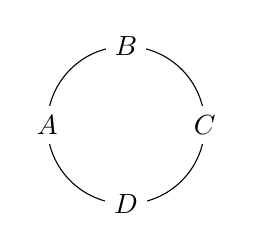
\begin{tikzpicture}
      \draw (0, 0) circle (1cm);
      \node at (1, 0) [fill=white] {$C$};
      \node at (0, 1) [fill=white] {$B$};
      \node at (-1, 0) [fill=white] {$A$};
      \node at (0, -1) [fill=white] {$D$};
    \end{tikzpicture}
    \hspace{1cm}
    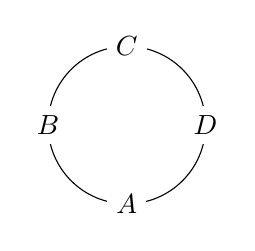
\begin{tikzpicture}
      \draw (0, 0) circle (1cm);
      \node at (1, 0) [fill=white] {$D$};
      \node at (0, 1) [fill=white] {$C$};
      \node at (-1, 0) [fill=white] {$B$};
      \node at (0, -1) [fill=white] {$A$};
    \end{tikzpicture}
  \end{center}
  \begin{center}
    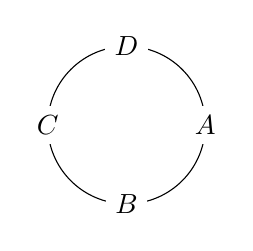
\begin{tikzpicture}
      \draw (0, 0) circle (1cm);
      \node at (1, 0) [fill=white] {$A$};
      \node at (0, 1) [fill=white] {$D$};
      \node at (-1, 0) [fill=white] {$C$};
      \node at (0, -1) [fill=white] {$B$};
    \end{tikzpicture}
    \hspace{1cm}
    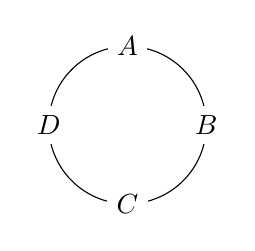
\begin{tikzpicture}
      \draw (0, 0) circle (1cm);
      \node at (1, 0) [fill=white] {$B$};
      \node at (0, 1) [fill=white] {$A$};
      \node at (-1, 0) [fill=white] {$D$};
      \node at (0, -1) [fill=white] {$C$};
    \end{tikzpicture}
  \end{center}

  From the above example, each circular permutation is correspended to 4 linear
  permutations. Given that the permutation of 4 people arranging in a row has
  $4!$ ways, so there are $\frac{4!}{4} = 3! = 6$ ways to arrange these four
  people in a circle.

  If we generalize the above example, we can get the following formula:

  \begin{enumerate}
    \item The formula of circular permutation of $n$ elements:
          \begin{cequation}
            \frac{\permtwo[n]{n}}{n} = \frac{n!}{n} = (n - 1)!
          \end{cequation}
    \item The formula of circular permutation of $r$ elements from $n$ elements ($r \leq
            n$):
          \begin{cequation}
            \frac{\permtwo[n]{r}}{r} = \frac{n!}{r(n - r)!}
          \end{cequation}
  \end{enumerate}

  \subsection{Practice 6}

  \begin{enumerate}
    \item Choose 5 people from 6 males and 5 females to be seated in a circle. How many
          ways can they be seated? \sol{}

          There are a total of $6+5 = 11$ people, so they are a total of
          $\frac{\permtwo[11]{5}}{5} = 11088$ ways to be seated.

    \item 6 males and 4 females are to be seated around a circular table. If females can't seat beside each other, how many ways can they be seated?
          \sol{}

          First, arrange the 6 males into a circle, there are $(6-1)! = 5!$ ways to do
          it. Next, arrange the the 4 females to sit in between the 6 males, there are
          $\permtwo[6]{4}$ ways to do it. So there are a total of $5! \cdot
            \permtwo[6]{4} = 120 \cdot 360 = 43200$ ways to arrange the seat.
  \end{enumerate}

  \subsection{Exercise 19.3}

  \begin{enumerate}
    \item 8 people are to be seated in a circle. How many ways can they be seated?
          \sol{}

          There are a total of $(8-1)! = 7! = 5040$ ways to arrange them.

    \item 10 children are to be arranged in a circle. How many ways can they be
          arraged? If a child must be seated in the primary position, how many ways can they be arranged?
          \sol{}

          There are a total of $(10-1)! = 9! = 362880$ ways to arrange them. If a child
          must be seated in the primary position, there are a total of $9! = 362880$ ways
          to arrange them.

    \item 6 people are to be formed into a circle. If two people must seat together, how many ways can they be arranged?
          \sol{}

          We can treat those two people as one person, so there are a total of $(5-1)! =
            4!$ ways to arrange them. Since these two people can switch their position, so
          there are a total of $2!$ ways to arrange them. Therefore, there are a total of
          $4! \cdot 2! = 24 \cdot 2 = 48$ ways to arrange them.

    \item 4 males and 3 females are to be seated around a circular table. If none of the females can seat together, how many ways can they be seated?
          \sol{}

          First, arrange the 4 males into a circle, there are $(4-1)! = 3!$ ways to do
          it. Next, put 3 females in between those 4 males, there are a total of
          $\permtwo[4]{3}$ ways to do it. So there are a total of $3! \cdot
            \permtwo[4]{3} = 6 \cdot 24 = 144$ ways to arrange the seat.

    \item 4 pairs of couples and one child are to be seated around a circular table. If the couples must sit together, how many ways can they be seated?
          \sol{}

          We can treat the couples as one person, so there are a total of $(3-1)! = 2!$
          ways to arrange them. Next, in between those couples, there are $4!$ ways to
          arrange them. Next, in between each couples, since they can switch their
          position, so there are a total of $2!$ ways to arrange them. Therefore, there
          are a total of $2! \cdot 4! \cdot 2! = 8 \cdot 24 \cdot 2 = 384$ ways to
          arrange them.

    \item A family of 7 people are sitting together around a circular table for a dinner.
          If the grandfather, grandmother, father and mother must sit together, of which
          the grandfather and the grandmother, the father and the mother must sit
          together, how many ways can they be seated? \sol{}

          Since grandfather, grandmother, father and mother must sit together, we can
          treat them as one person, so there are a total of $(4-1)! = 3!$ ways to arrange
          them. In between those 4 people who must be seated together, since the
          grandfather and the grandmother, the father and the mother can switch their
          position, so there are a total of $2!$ ways to arrange them. Next, in between
          the grandfather and grandmother, father and mother, since they can switch their
          position, so there are a total of $2 \cdot 2!$ ways to arrange them. Therefore,
          there are a total of $3! \cdot 2! \cdot 2 \cdot 2! = 48$ ways to arrange them.

    \item If a linear permutation of $n$ people is 6 times of a circular permutation of
          $n$ people, find these two permutations. \sol{}
          \begin{flalign*}
            n!                     & = 6(n-1)! \\
            \frac{n!}{(n-1)!}      & = 6       \\
            \frac{n(n-1)!}{(n-1)!} & = 6       \\
            n                      & = 6
          \end{flalign*}
          So there are a total of $6! = 720$ linear permutations and $(6-1)! = 5! = 120$ circular permutations.
  \end{enumerate}

  \section{Full Permutations of Inexactly Distinct Elements}

  In all the previous questions of permutations, the given elements are all
  distinct. However, in some cases, there are some elements that are the same,
  this kind of permutation are considered as \emph{permutations with repetition}.
  Let's discusse the folowing example:

  For a full permutation of three elements $a$, $a$, and $b$, how many ways can
  they be arranged?

  Let's treat the identical elemnents $a$ as two different elements $a_1$ and
  $a_2$, there will be 3! ways to arrange these three different element $a_1$,
  $a_2$, and $b$, as listed below:

  \begin{center}
    $a_1 \quad a_2 \quad b \qquad a_2 \quad a_1 \quad b$

    $a_1 \quad b \quad a_2 \qquad a_2 \quad b \quad a_1$

    $b \quad a_1 \quad a_2 \qquad b \quad a_2 \quad a_1$
  \end{center}

  In the three rows above, for each row, the position of $b$ is fixed, $a_1$ and
  $a_2$ has $2! = 2$ ways to be arranged.

  If we change $a_1$ and $a_2$ above back to $a$, then the two different
  arrangements of $a_1$ and $a_2$ will be counted as one arrangement of $a$.
  Hence, there are only $\frac{3!}{2!} = 3$ ways for full permutation of three
  elements $a$, $a$, and $b$.

  Generalize the above example, given $n$ elements, where there are $n_1$
  elements $a_1$, $n_2$ elements $a_2$, $\cdots$, $n_k$ elements $a_k$, where
  $n_1 + n_2 + \cdots + n_k = n$, then the number of full permutations of these
  $n$ elements is:
  \begin{cequation}
    \frac{n!}{n_1!n_2!\cdots n_k!}
  \end{cequation}

  \subsection{Practice 7}

  \begin{enumerate}
    \item Giving 9 children 2 pens, 3 ball-point pens, 4 pencils, how many ways can they
          be given if each child must be given one pen? \sol{}

          There are a total of $\frac{9!}{2!3!4!} = 1260$ ways to give the children the
          pens.

    \item Find the full permutation of the letters in the word \textit{EXPRESSION} with 9
          letters. \sol{} There are 2 $E$s, 2 $S$s, 1 $P$, 1 $O$, 1 $N$, 1 $R$ and 1 $X$.
          Hence, there are a total of $\frac{10!}{2!2!1!1!1!1!} = 907200$ ways to arrange
          the letters in the word \textit{EXPRESSION}.
  \end{enumerate}

  \subsection{Exercise 19.4}

  \begin{enumerate}
    \item How many 8 digit numbers can be formed using 8 digits 1, 1, 2, 2, 3, 3, 4, 5?
          \sol{}

          There are 2 $1$s, 2 $2$s, 2 $3$s, 1 $4$ and 1 $5$ in these 8 digits. Hence,
          there are a total of $\frac{8!}{2!2!2!1!1!} = 5040$ ways to arrange the 8
          digits.

    \item Arranging all the letters in the word \textit{MALAYSIA}, how many ways can they
          be arranged such that the three "A"s are not totally together? \sol{}

          There are 3 $A$s, 1 $L$, 1 $M$, 1 $S$, 1 $I$ and 1 $Y$ in the word
          \textit{MALAYSIA}. Hence, there are a total of $\frac{8!}{3!1!1!1!1!1!} = 6720$
          ways to arrange the letters in the word \textit{MALAYSIA}. If all the $A$s are
          together, treat all the $A$ as one element, there are $6! = 720$ ways to
          arrange them. Hence, there are a total of $6720 - 720 = 6000$ ways to arrange
          the letters in the word \textit{MALAYSIA} such that the three "A"s are not
          totally together.

    \item Arranging all the letters in the word \textit{MATHEMATICAL}, how many ways can
          they be arranged such that the three "A"s are not totally together? \sol{}

          There are 3 $A$s, 2 $M$s, 2 $T$s, 1 $C$, 1 $E$, 1 $H$, 1 $I$, 1 $L$, and 1 $U$
          in the word \textit{MATHEMATICAL} with 12 letters. There are a total of
          $\frac{12!}{3!2!2!1!1!1!1!1!1!} = 19958400$ ways to arrange the letters in the
          word. If all the $A$s are together, treat all the $A$ as one element, there are
          $\frac{10!}{2!2!1!1!1!1!1!} = 907200$ ways to arrange them. Hence, there are a
          total of $19958400 - 907200 = 19051200$ ways to arrange the letters in the word
          \textit{MATHEMATICAL} such that the three "A"s are not totally together.

    \item The diagram below shows a city with 5 north-west roads and 5 south-east roads,
          where each road shares the same length.
          \begin{center}
            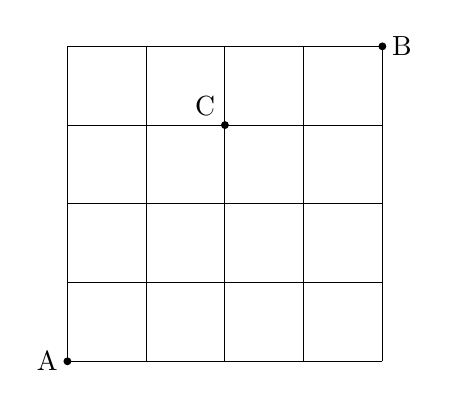
\begin{tikzpicture}
              \draw (0, 0) -- (0, 4);
              \draw (1, 0) -- (1, 4);
              \draw (2, 0) -- (2, 4);
              \draw (3, 0) -- (3, 4);
              \draw (4, 0) -- (4, 4);
              \draw (0, 0) -- (4, 0);
              \draw (0, 1) -- (4, 1);
              \draw (0, 2) -- (4, 2);
              \draw (0, 3) -- (4, 3);
              \draw (0, 4) -- (4, 4);
              \fill (0, 0) circle (0.05);
              \fill (2, 3) circle (0.05);
              \fill (4, 4) circle (0.05);
              \node at (0, 0) [left] {A};
              \node at (2, 3) [above left] {C};
              \node at (4, 4) [right] {B};
            \end{tikzpicture}
          \end{center}
          \begin{enumerate}
            \item How many shortest paths are there from $A$ through $C$ to $B$? \sol{}

                  From $A$ to $C$, we must walk 3 steps to the north and 2 steps to the east.
                  There are a total of $\frac{5!}{3!2!} = 10$ ways go from $A$ to $C$.

                  From $C$ to $B$, we must walk 1 step to the north and 2 steps to the east.
                  There are a total of $\frac{3!}{1!2!} = 3$ ways go from $C$ to $B$.

                  Hence, there are a total of $10 \cdot 3 = 30$ shortest paths from $A$ through
                  $C$ to $B$.

            \item How many shortest paths are there from A to B without passing through C? \sol{}

                  From $A$ to $B$, we must walk 4 steps to the north and 4 steps to the east.
                  There are a total of $\frac{8!}{4!4!} = 70$ ways go from $A$ to $B$.

                  Hence, there are a total of $70 - 30 = 40$ shortest paths from $A$ to $B$
                  without passing through $C$.
          \end{enumerate}

    \item Arranging all the letters in the word \textit{GEOMETRIC}, find the number of
          permutations such that the following conditions are satisfied:
          \begin{enumerate}
            \item No limitaion on the arrangement of the letters. \sol{}

                  There are 2 $E$s, 1 $G$, 1 $I$, 1 $M$, 1 $O$, 1 $R$, 1 $C$, and 1 $T$ in the
                  word \textit{GEOMETRIC} with 9 letters. There are a total of
                  $\frac{9!}{2!1!1!1!1!1!1!1!} = 181400$ ways to arrange the letters in the word.

            \item All the vowels must be together. \sol{}

                  Treat all vowels as one element, there are $6! = 720$ ways to arrange them.
                  since all vowels can switch position with each other, there are
                  $\frac{4!}{2!1!1!} = 12$ ways to arrange them. Hence, there are a total of $720
                    \cdot 12 = 8640$ ways to arrange the letters in the word \textit{GEOMETRIC}
                  such that all the vowels are together.

            \item None of the vowels are adjacent to each other. \sol{}

                  Arrange all the consonants together. There are $5! = 120$ ways to arrange them.
                  Next, put 4 vowels at the beginning of the word, the end of the word, or in
                  between consonants. There are a total of $\frac{\permtwo[6]{4}}{2!1!1!} = 180$
                  ways to do so. Hence, there are a total of $120 \cdot 180 = 21600$ ways to
                  arrange the letters in the word \textit{GEOMETRIC} such that none of the vowels
                  are adjacent to each other.
          \end{enumerate}

  \end{enumerate}

  \section{Permutations with Repetition}

  If the elements can be chosen more than once, arranging $r$ elements from $n$
  elements is called \emph{permutation with repetition} of $r$ elements from $n$
  elements.

  Given $n$ distinct elements, each element can be chosen more than once, then
  there are $n$ ways to choose the first element, $n$ ways to choose the second
  element, $\cdots$, $n$ ways to choose the $r$th element. According to the
  multiplication rule, its permutations are:
  \begin{cequation}
    \underbrace{n \cdot n \cdot \cdots \cdot n}_{r} = n^r
  \end{cequation}

  \subsection{Practice 8}

  \begin{enumerate}
    \item How many ways are there to shoot 3 balls into 6 baskets? \sol{}

          There are 6 baskets, each basket can be shoot more than once, so there are $6^3
            = 216$ ways to shoot 3 balls into 6 baskets.

    \item If the all the digits can be used more than once, how many 3 digit numbers can
          be formed using the digits 0, 1, 2, 3, 4? \sol{}

          Since the first digit cannot be 0, there are 4 ways to choose it. For the other
          two digits, there are 5 ways to choose each of them. Hence, there are a total
          of $4 \cdot 5 \cdot 5 = 100$ 3 digit numbers can be formed using the digits 0,
          1, 2, 3, 4.
  \end{enumerate}

  \subsection{Exercise 19.5}

  \begin{enumerate}
    \item The office documents of a company are coded with a combination of two of the
          first four letters of the alphabet $A, B, C, D$. If each letter can be used
          more than once, how many different codes can be formed? \sol{}

          There are two letters in each code, each letter can be chosen more than once,
          so there are $4^2 = 16$ different codes can be formed.

    \item There are eight paths from A to B. How many ways are there to go from A to B
          and then back to A? \sol{}

          There are 8 paths from A to B, and 8 paths from B to A. Hence, there are a
          total of $8 \cdot 8 = 64$ ways to go from A to B and then back to A.

    \item A four digit number is to be formed with 4 numbers 3, 4, 5, 7, how many ways
          can it be formed such that its thousand digit and hundred digit are the same?
          \sol{}

          Since the thousand digit and hundred digit are the same, there are 4 ways to
          choose the thousand and hundred digit combined. For the other two digits, there
          are 4 ways to choose each of them. Hence, there are a total of $4 \cdot 4 \cdot
            4 = 64$ ways to form a four digit number such that its thousand digit and
          hundred digit are the same.

    \item A basketball match has two possible result, either team $A$ wins or team $B$
          wins. How many possible results are there if there are 10 matches? \sol{}

          There are 2 possible results, either team $A$ wins or team $B$ wins. Hence,
          there are a total of $2^{10} = 1024$ possible results if there are 10 matches.

    \item A restaurant has introduced 7 sets of special dishes for lunch. There are 3
          people come for lunch, each person orders one dish. How many different
          combinations of dishes can be ordered? \sol{}

          There are 7 sets of special dishes, each person can order any of the 7 dishes.
          Hence, there are a total of $7^3 = 343$ different combinations of dishes can be
          ordered.

    \item A building is assigned one security guard every night. If the security company
          has three assignable guards, how many different ways of assignments are there
          for a week? \sol{}

          There are 7 nights in a week, each night can be assigned to any of the 3
          guards. Hence, there are a total of $3^7 = 2187$ different ways of assignments
          are there for a week.

    \item A football match has three possible results, either team $A$ wins, team $B$
          wins or the match is a draw. How many possible results are there if there are 8
          matches?

          There are 3 possible results, either team $A$ wins, team $B$ wins or the match
          is a draw. Hence, there are a total of $3^{8} = 6561$ possible results if there
          are 8 matches.

    \item A school is going to hold a trilingual speech competition. The rule stated that
          each class can only send one representative for each language. If there are 40
          students in a class, how many different combinations of students can be chosen
          for the competition? \sol{}

          There are 3 languages, each class can only send one representative for each of
          the 3 languages. Hence, there are a total of $40^3 = 64000$ different
          combinations of students can be chosen for the competition.

    \item How many 6 digits odd number can be formed using the digitis 0, 1, 2, $\cdots$,
          5 if each digit can be used more than once? \sol{}

          Since the number is odd, the last digit must be odd. Hence, there are 3 ways to
          choose it. Since the first digit cannot be 0, there are 5 ways to choose it.
          For the other four digits, there are 6 ways to choose each of them. Hence,
          there are a total of $3 \cdot 5 \cdot 6^4 = 19440$ 6 digits odd number can be
          formed using the digitis 0, 1, 2, $\cdots$, 5 if each digit can be used more
          than once.

    \item The phone number format of a country is going from 7 digits to 8 digits. but
          the leading digit cannot be 0 or 1. How many new phone numbers will be formed
          after the change? \sol{}

          When there are only 7 digits, there are 8 ways to choose the first digit (2 -
          10), 10 ways to choose the rest of the digits (0 - 10). Hence, there are $8
            \cdot 10^6$ phone numbers. When there are 8 digits, there are 8 ways to choose
          the first digit, 10 ways to choose the rest of the digits. Hence, there are $8
            \cdot 10^7$ phone numbers. Hence, there are:
          \begin{flalign*}
            8 \cdot 10^7 - 8 \cdot 10^6 & = 80,000,000 - 8,000,000 \\
                                        & = 72,000,000
          \end{flalign*}
          new phone numbers.
  \end{enumerate}

  \section{Combinations and Combination Formula}

  Grouping $r$ elements from $n$ elements ($r \leq n$) without considering the
  order of the elements is called \emph{combination} of $r$ elements from $n$
  elements. The number of combinations of $r$ elements from $n$ elements is
  denoted by $\combtwo[n]{r}$, $\comb[n]{r}$, or $\binom{n}{r}$.

  Take for example: taking two elements from three distinct element $a$, $b$, $c$
  to form a group. Below are the combinations of any two elements from $a$, $b$,
  $c$:
  \begin{center}
    \begin{tabular}{|c|c|c|c|c|c|c|}
      \hline
      Permutations & $ab$                      & $ba$                      & $ac$                      & $ca$ & $bc$ & $cb$ \\
      \hline
      Combinations & \multicolumn{2}{c|}{$ab$} & \multicolumn{2}{c|}{$ac$} & \multicolumn{2}{c|}{$bc$}                      \\
      \hline
    \end{tabular}
  \end{center}

  It can be considered as two steps:

  First, combine any two elements from the three distinct elements to form a
  group. There are $\comb[3]{2}$ possible combinations.

  Second, make full permutations for each combination. There are $2!$ possible
  permutations for each combination.

  According to the multiplication rule,
  \begin{flalign*}
    \permtwo[3]{2}            & = \comb[3]{2} \cdot 2!      \\
    \therefore\ \ \comb[3]{2} & = \frac{\permtwo[3]{2}}{2!} \\
                              & = 3
  \end{flalign*}

  Generalizing the above example, there are two steps to find the combinations of
  $r$ elements from $n$ elements:

  First, combine any $r$ elements from the $n$ elements to form a group. There
  are $\comb[n]{r}$ possible combinations.

  Second, make full permutations for each combination. There are $r!$ possible
  permutations for each combination.

  According to the multiplication rule,
  \begin{flalign*}
    \permtwo[n]{r}            & = \comb[n]{r} \cdot r!              \\
    \therefore\ \ \comb[n]{r} & = \frac{\permtwo[n]{r}}{r!}         \\
                              & = \frac{n!}{(n - r)! r!},\ r \leq n
  \end{flalign*}

  According to the definition $\comb[n]{r} = \frac{n!}{(n - r)! r!}$,
  \begin{flalign*}
    \comb[n]{n-r} & = \frac{n!}{(n - (n - r))! (n - r)!} \\
                  & = \frac{n!}{r! (n - r)!}             \\
                  & = \comb[n]{r}
  \end{flalign*}

  That is,
  \begin{cequation}
    \comb[n]{r} = \comb[n]{n - r}
  \end{cequation}

  Note that:
  \begin{enumerate}
    \item If $r = n$, then $\comb[n]{n} = \frac{n!}{0! n!} = 1$.
    \item If $r = 0$, then $\comb[n]{0} = \frac{n!}{n! 0!} = 1$.
  \end{enumerate}

  \subsection{Practice 9}

  \begin{enumerate}
    \item There are six main cities in a country, each city has roads connecting to the
          other five cities. How many roads are there connecting the six cities? \sol{}

          a road is formed between 2 cities, there are $\comb[6]{2} = 15$ roads
          connecting the six cities.

    \item 5 people are to be distributed in 4 cars, each car must have at least one person. How many
          ways are there to distribute the 5 people into 4 cars? \sol{}

          There are one car with two people, so there are $\comb[5]{2} = 10$ ways of
          distribution. For these 3 people and one group of 2 people, there are
          $\permtwo[4]{4} = 4! = 24$ ways of distribution. Hence, there are $10 \cdot 24
            = 240$ ways of distributing the 5 people into 4 cars.

  \end{enumerate}

  \subsection{Practice 10}

  There are 4 different books. With the following criteria, how many ways are
  there to distribute the books?
  \begin{enumerate}[label=(\alph*)]
    \item Distribute evenly to two people. \sol{}

          First, distribute the book to one person. There are $\comb[4]{2} = 6$ ways of
          distribution. Then, distribute the remaining books to the other person. There
          are $\comb[2]{2} = 1$ way of distribution. Hence, there are $N_1 = 6 \cdot 1 =
            6$ ways of distributing the books.

    \item Seperate evenly into two piles. \sol{}

          Destructing the solution of (a). First, distribute the book into two piles.
          There are $N_2$ ways of distribution. Then, distribute each pile to the two
          people. There are $2!$ ways of distribution. There are $N_1 = N_2 \cdot 2!$
          ways of distributing the books. Hence, there are $N_2 = \frac{6}{2!} = 3$ ways
          of distributing the books into two piles.
  \end{enumerate}

  \subsection{Exercise 19.6}

  \begin{enumerate}
    \item Find the value of $n$ and $r$ of the following expessions:
          \begin{enumerate}
            \item $\comb[16]{r+3} = \comb[16]{7-r}$
                  \sol{}
                  \begin{flalign*}
                    \comb[16]{r+3} & = \comb[16]{7-r} \\
                    r+3            & = 7-r            \\
                    2r             & = 4              \\
                    r              & = 2
                  \end{flalign*}

            \item $\comb[30]{r} = \comb[30]{r+2}$
                  \sol{}
                  \begin{flalign*}
                    \comb[30]{r} & = \comb[30]{r+2} \\
                    30 - r       & = r + 2          \\
                    2r           & = 28             \\
                    r            & = 14
                  \end{flalign*}

            \item $\comb[n]{8} = \comb[n]{7}$
                  \sol{}
                  \begin{flalign*}
                    \comb[n]{8} & = \comb[n]{7}   \\
                    \comb[n]{r} & = \comb[n]{n-r} \\
                    r           & = 8             \\
                    n-r         & = 7             \\
                    n - 8       & = 7             \\
                    n           & = 15
                  \end{flalign*}
          \end{enumerate}

    \item Assume that $3(\comb[n]{4}) = 5(\comb[n-1]{5})$, find the value of
          $\comb[n]{9}$. \sol{} \setlength{\belowdisplayskip}{0pt}
          \setlength{\belowdisplayshortskip}{0pt} \setlength{\abovedisplayskip}{0pt}
          \setlength{\abovedisplayshortskip}{0pt}
          \begin{flalign*}
            3(\comb[n]{4})                                                                   & = 5(\comb[n-1]{5}) \\
            \frac{\comb[n]{4}}{\comb[n-1]{5}}                                                & = \frac{5}{3}      \\
            \frac{n!}{4!(n-4)!} \cdot \frac{5!(n-6)!}{(n-1)!}                                & = \frac{5}{3}      \\
            \frac{n(n-1)!}{4!(n-4)!} \cdot \frac{5\cdot 4!(n-6)!}{(n-1)!}                    & = \frac{5}{3}      \\
            \frac{5n(n-6)!}{(n-4)!}                                                          & = \frac{5}{3}      \\
            \frac{5n(n-6)!}{(n-4)(n-5)(n-6)!}                                                & = \frac{5}{3}      \\
            \frac{n}{(n-4)(n-5)}                                                             & = \frac{1}{3}      \\
            3n                                                                               & = (n-4)(n-5)       \\
            n^2 - 9n + 20 - 3n                                                               & = 0                \\
            n^2 - 12n + 20                                                                   & = 0                \\
            (n-10)(n-2)                                                                      & = 0                \\
            n                                                             = 10 \text{ or } n & = 2
          \end{flalign*}
          \begin{flalign*}
            \because\    & n \in \mathbb{N},\ n > 6 \\
            \therefore\  & n = 10
          \end{flalign*}
          \begin{flalign*}
            \comb[n]{9} & = \comb[10]{9}           \\
                        & = \frac{10!}{9!(10-9)!}  \\
                        & = \frac{10!}{9!1!}       \\
                        & = \frac{10 \cdot 9!}{9!} \\
                        & = 10
          \end{flalign*}
          \setlength{\belowdisplayskip}{\baselineskip} \setlength{\belowdisplayshortskip}{\baselineskip}
          \setlength{\abovedisplayskip}{\baselineskip} \setlength{\abovedisplayshortskip}{\baselineskip}

    \item There are 17 teams participating in a football competition. If each team plays
          against every other team, how many matches are there? \sol{}

          Choosing two teams from 17 teams. There are $\comb[17]{2} = 136$ ways of
          matching.

    \item How many diagonals can be drawn in a convex nonagon? \sol{}

          There are 9 vertices in a nonagon. Since the diagonals do not include the 9
          sides of the nonagon, there are $\comb[9]{2} - 9 = 36 - 9 = 27$ diagonals in a
          nonagon.

    \item There are 6 students on duty in a class, 1 student is in charge of cleaning the
          whiteboard, 1 is in charge of cleaning the rubbish bin, 2 students are in
          charge of sweeping the floor and 2 students are in charge of arranging the
          desks. How many ways are there to distribute the 6 students into the 4 jobs?
          \sol{}

          To choose 1 from 6 students for cleaning the whiteboard, there are $\comb[6]{1}
            = 6$ ways. To choose 1 from 5 students for cleaning the rubbish bin, there are
          $\comb[5]{1} = 5$ ways. To choose 2 from 4 students for sweeping the floor,
          there are $\comb[4]{2} = 6$ ways. The two students left will be in charge of
          arranging the desks. Therefore, there are $\comb[6]{1} \cdot \comb[5]{1} \cdot
            \comb[4]{2} = 6 \cdot 5 \cdot 6 = 180$ ways to distribute the 6 students into
          the 4 jobs.

    \item 4 people are to be choosen from 5 couples, where each couple cannot be chosen together. How many ways are there to choose the 4 people?
          \sol{}

          Choosing 4 people from 10 people or 5 couples with no restriction, there are
          $\comb[10]{4}$ ways. Choosing 4 people with at least one couple, there are
          $\comb[5]{1} \cdot \comb[8]{2}$ ways. Choosing 4 people with two couples, there
          are $\comb[5]{2}$ ways. Therefore, using inclusion-exclusion principle, there
          are $\comb[10]{4} - \comb[5]{1} \cdot \comb[8]{2} + \comb[5]{2} = 210 - 140 +
            10 = 80$ ways to choose 4 people from 5 couples where each couple cannot be
          chosen together.

    \item Three signal flags are to be chosen from 6 flags, one of which is red, two of
          which are yellow and the rest are blue. How many ways are there to choose the 3
          flags? \sol{}

          Choosing 1 flag from each color, there are $\comb[1]{1} \cdot \comb[2]{1} \cdot
            \comb[3]{1} = 6$ ways. Choosing 1 red and 2 yellow, there are $1 \cdot
            \comb[2]{2} = 1$ ways. Choosing 1 red and 2 blue, there are $1 \cdot
            \comb[3]{2} = 3$ ways. Choosing 2 yellow and 1 blue, there are $\comb[2]{2}
            \cdot 1 = 2$ ways. Choosing 1 yellow and 2 blue, there are $\comb[2]{1} \cdot
            \comb[3]{2} = 6$ ways. Choosing 3 blue, there are $\comb[3]{3} = 1$ way.
          Therefore, there are $6 + 1 + 3 + 2 + 6 + 1 = 19$ ways to choose 3 flags from 6
          flags.

    \item A delegation with 6 members is to be formed from 9 students who major in
          Mathematics and 4 students who major in Education. With the following criteria,
          how many ways are there to form the delegation?
          \begin{enumerate}
            \item There are exactly two students who major in Education. \sol{}

                  Choose 2 from 4 students who major in Education, there are $\comb[4]{2}$ ways.
                  Choose the other 4 students from 9 students who major in Mathematics, there are
                  $\comb[9]{4}$ ways. Therefore, there are $\comb[4]{2} \cdot \comb[9]{4} = 6
                    \cdot 126 = 756$ ways to form the delegation.

            \item There are at least two students who major in Education. \sol{}

                  According to the critera, the combination of less than two students who major
                  in Education is not allowed. There are a total of $\comb[13]{6}$ ways to form
                  the delegation with no restriction, and there are $\comb[9]{6}$ ways to form
                  the delegation with no Education major, $\comb[4]{1} \cdot \comb[9]{5}$ ways to
                  form the delegation with one Education major. Therefore, there are
                  $\comb[13]{6} - \comb[9]{6} - \comb[4]{1} \cdot \comb[9]{5} = 1716 - 84 - 504 =
                    1118$ ways to form the delegation with at least two Education majors.

          \end{enumerate}

    \item Separate 14 students evenly into 2 groups, how many ways are there to do so?
          How many ways are there to seperate these 14 students evenly into two
          classrooms? \sol{}

          Choose 7 students from 14 students to form a group, there are $\comb[14]{7}$
          ways. Since the order of the groups does not matter, there are
          $\frac{\comb[14]{7}}{2!} = \frac{3432}{2} = 1716$ ways of seperating 14
          students evenly into 2 groups.

          If the 14 students are to be seperated into two classrooms, since the these two
          groups of stuents can switch classrooms, there are $1716 \cdot 2! = 3432$ ways
          to do so.

  \end{enumerate}

  \section{Revision Exercise 19}

  \begin{enumerate}
    \item Evaluate the following:
          \begin{enumerate}
            \item $\frac{7!}{3!4!} + \frac{7!}{2!5!}$
                  \sol{}
                  \begin{flalign*}
                    \frac{7!}{3!4!} + \frac{7!}{2!5!} & = \frac{7 \cdot 6 \cdot 5!}{6 \cdot 24} + \frac{7 \cdot 6 \cdot 5!}{2 \cdot 120} \\
                                                      & = \frac{7 \cdot 5!}{24} + \frac{7 \cdot 5!}{40}                                  \\
                                                      & = \frac{7 \cdot 120}{24} + \frac{7 \cdot 120}{40}                                \\
                                                      & = 7 \cdot 5 + 7 \cdot 3                                                          \\
                                                      & = 35 + 21                                                                        \\
                                                      & = 56
                  \end{flalign*}

            \item $\frac{\permtwo[11]{5} + \permtwo[11]{4}}{\permtwo[12]{5} + \permtwo[12]{4}}$\\
                  \sol{}
                  \begin{flalign*}
                    \frac{\permtwo[11]{5} + \permtwo[11]{4}}{\permtwo[12]{5} + \permtwo[12]{4}} & = \frac{\frac{11!}{(11-5)!} + \frac{11!}{(11-4)!}}{\frac{12!}{(12-5)!} + \frac{12!}{(12-4)!}} \\
                                                                                                & = \frac{\frac{11!}{6!} + \frac{11!}{7!}}{\frac{12!}{7!} + \frac{12!}{8!}}                     \\
                                                                                                & = \frac{\frac{11!(6!+7!)}{6!7!}}{\frac{12!(7!+8!)}{7!8!}}                                     \\
                                                                                                & = \frac{11!(6!+7!)}{6!7!} \cdot \frac{7!8!}{12!(7!+8!)}                                       \\
                                                                                                & = \frac{11!(6!+7!)}{6!} \cdot \frac{8 \cdot 7 \cdot 6!}{12!(7!+8!)}                           \\
                                                                                                & = \frac{56 \cdot 11!(6!+7!)}{12 \cdot 11!(7!+8!)}                                             \\
                                                                                                & = \frac{14(6!+7!)}{3(7!+8!)}                                                                  \\
                                                                                                & = \frac{14(6!+7 \cdot 6!)}{3(7!+8 \cdot 7!)}                                                  \\
                                                                                                & = \frac{14\cdot 6! \cdot 8}{3 \cdot 7! \cdot 9}                                               \\
                                                                                                & = \frac{14\cdot 6! \cdot 8}{3 \cdot 7 \cdot 6! \cdot 9}                                       \\
                                                                                                & = \frac{14 \cdot 8}{3 \cdot 7 \cdot 9}                                                        \\
                                                                                                & = \frac{2 \cdot 8}{3 \cdot 9}                                                                 \\
                                                                                                & = \frac{16}{27}                                                                               \\
                  \end{flalign*}
          \end{enumerate}

    \item If $\frac{(n+6)!}{(n+4)!} = 18(n+1)$, find the value of $n$. \sol{}
          \begin{flalign*}
            \frac{(n+6)!}{(n+4)!}                             & = 18(n+1)  \\
            \frac{(n+6)(n+5)(n+4)!}{(n+4)!}                   & = 18(n+1)  \\
            (n+6)(n+5)                                        & = 18(n+1)  \\
            n^2 + 11n + 30                                    & = 18n + 18 \\
            n^2 -7n + 12                                      & = 0        \\
            (n-3)(n-4)                                        & = 0        \\
            n                               = 3 \text{ or } n & = 4
          \end{flalign*}

    \item Assume that $\comb[2n]{3}:\comb[n]{2} = 44:3$, find the value of $n$. \sol{}
          \begin{flalign*}
            \comb[2n]{3}:\comb[n]{2}                                     & = 44:3         & \\
            \frac{\comb[2n]{3}}{\comb[n]{2}}                             & = \frac{44}{3}   \\
            \frac{(2n!)}{3!(2n-3)!} \cdot \frac{2!(n-2)!}{n!}            & = \frac{44}{3}   \\
            \frac{(2n!)}{6(2n-3)!} \cdot \frac{2(n-2)!}{n!}              & = \frac{44}{3}   \\
            \frac{(2n!)}{3(2n-3)!} \cdot \frac{(n-2)!}{n!}               & = \frac{44}{3}   \\
            \frac{(2n!)}{(2n-3)!} \cdot \frac{(n-2)!}{n!}                & = 44             \\
            \frac{(2n!)}{(2n-3)!} \cdot \frac{(n-2)!}{n(n-1)(n-2)!}      & = 44             \\
            \frac{2n(2n-1)(2n-2)(2n-3)!}{(2n-3)!} \cdot \frac{1}{n(n-1)} & = 44             \\
            \frac{4n(2n-1)(n-1)}{n(n-1)}                                 & = 44             \\
            4(2n-1)                                                      & = 44             \\
            2n - 1                                                       & = 11             \\
            2n                                                           & = 12             \\
            n                                                            & = 6
          \end{flalign*}

    \item All the letters from the word \textit{TRIANGLE} are to be arranged. How many
          ways of arrangements are there such that the vowels are all seperated from each
          other? \sol{}

          First, arrange the consonants. There are $\permtwo[5]{5} = 5!$ ways to do so.
          Then, put the vowels in the beginning of the word, the end of the word, or in
          between the consonants. There are $\permtwo[6]{3}$ ways to do so. Thus, there
          are $\permtwo[6]{3} \cdot 5! = 120 \cdot 120 = 14400$ ways to arrange the
          letters.

    \item One vowel and one consonant are to be chosen from the word \textit{VOLUME} to
          form a word. How many ways are there to do so? \sol{}

          There are 3 consonants and 3 vowels. Pick one from each of them, there are 9
          ways. Since the consonant and vowel can be chosen in any order, there are $9
            \cdot 2 = 18$ ways.

    \item A basketball coach wants to choose two vanguards from four shooters, one center
          from two tall players, and two defenders from four ball handlers. How many ways
          are there to form a team? \sol{}

          There are $\comb[4]{2} = 6$ ways to choose two vanguards, $\comb[2]{1} = 2$
          ways to choose one center, and $\comb[4]{2} = 6$ ways to choose two defenders.
          Thus, there are $6 \cdot 2 \cdot 6 = 72$ ways to form a team.

    \item A committee must be formed by one lawyer, two engineers and two doctors chosen
          from 3 lawyers, 6 engineers and 7 doctors. How many ways are there to form the
          committee? \sol{}

          There are $\comb[3]{1} = 3$ ways to choose one lawyer, $\comb[6]{2} = 15$ ways
          to choose two engineers, and $\comb[7]{2} = 21$ ways to choose two doctors.
          Thus, there are $3 \cdot 15 \cdot 21 = 945$ ways to form the committee.

    \item  There is one of each note of the following value: \$1, \$5, \$10, \$20, \$50,
          \$100. How many distinct values of currency can be made from these notes?

          \sol{}

          Pick one note, there are $\comb[6]{1} = 6$ ways to do so.

          Pick two notes, there are $\comb[6]{2} = 15$ ways to do so.

          \vdots

          Pick six notes, there are $\comb[6]{6} = 1$ way to do so.

          Thus, there are $6 + 15 + 20 + 15 + 6 + 1 = 63$ distinct values of currency
          that can be made from these notes.

    \item There are 4 different history books, 5 different geography books and 3
          different literature books on the shelf. If they are to be arranged in a row,
          how many ways are there to arrange them such that books of the same subject are
          arranged together?

          \sol{}

          There are $\permtwo[4]{4} = 4!$ ways to arrange the history books.

          There are $\permtwo[5]{5} = 5!$ ways to arrange the geography books.

          There are $\permtwo[3]{3} = 3!$ ways to arrange the literature books.

          Since the books of each subject can be arranged in any order, there are $3!
            \cdot 4! \cdot 5! \cdot 3! = 6 \cdot 24 \cdot 120 \cdot 6 = 103680$ ways to
          arrange the books.

    \item 6 characters from 10 different characters $A$, $B$, $C$, $D$, $E$, and 0, 1, 2, 3, 4 are to be chosen to form a password. How many password can be formed such that there are no repeated characters and the password does not start with 0?
          \sol{}

          Since the first character cannot be 0, there are 9 ways to choose the first
          character. Since there are 2 categories of characters: alphabets and digits,
          there are $\frac{\permtwo[10]{5}}{2}$ ways to choose the remaining 5
          characters. Thus, there are $9 \cdot \frac{\permtwo[10]{5}}{2} = 9 \cdot 151020
            = 136080$ passwords that can be formed.

    \item How many 7 digit even numbers can be formed from full permutations of the
          digits 0, 1, 2, 3, 4, 5, 6? How many multiple of 10 are there in these numbers?
          \sol{}

          Since the first digit cannot be 0, there are 6 ways to choose the first digit,
          3 even and 3 odd. Since the number must be even, the last digit must be 2, 4,
          6, or 0. If the first digit is even, there are 3 ways to choose the last digit.
          If the first digit is odd, there are 4 ways to choose the last digit. Thus,
          there are $3 \times 3 + 3 \times 4 = 21$ ways to choose the first and the last
          digit. For the other 5 digits, there are $\permtwo[5]{5} = 5!$ ways to choose
          them. Thus, there are $21 \cdot 5! = 21 \cdot 120 = 2520$ 7 digit even numbers
          that can be formed.

    \item How many permutations of all the characters in the word "fei li wu shi, fei li
          wu ting" are there? \sol{}

          There are 2 "fei"s, 2 "li"s, 2 "wu"s, 1 "shi", and 1 "ting". Therefore, there
          are $\frac{8!}{2!2!2!1!1!} = 5040$ permutations of all the characters in the
          word "fei li wu shi, fei li wu ting".

    \item How many ways are there to arrange all the letters in the word
          \textit{ARRANGEMENT}? \sol{}

          There are 2 "A"s, 2 "R"s, 2 "N"s, 1 "G", 2 "E"s, 1 "M", and 1 "T". Therefore,
          there are $\frac{11!}{2!2!2!2!1!1!1!} = 2494800$ ways to arrange all the
          letters in the word \textit{ARRANGEMENT}.

    \item Arranging 6 cups with different color and 4 canned juices with different
          flavour into a circle, how many ways are there to do so such that all the
          canned juices are not next to each other? \sol{}

          First, arrange the 6 cups into a circle. There are $(6-1)! = 5!$ ways of doing
          so.

          Then, arrange the 4 canned juices in between the cups. There are
          $\permtwo[6]{4}$ ways of doing so.

          Thus, there are $5! \cdot \permtwo[6]{4} = 120 \cdot 360 = 43200$ ways to
          arrange the 6 cups and 4 canned juices into a circle such that all the canned
          juices are not next to each other.

    \item In a box of Chinese chess, there are 1 general, 2 advisors, 2 elephants, 2
          horses, 2 chariots, 2 cannons and 5 soldiers of red color. Now we arrange these
          16 pieces into a circle:
          \begin{enumerate}
            \item All the pieces of the same type are arranged together. \sol{}

                  There are 7 types of pieces. Thus, there are $(7-1)! = 6! = 720$ ways to
                  arrange the 7 types of pieces into a circle.

            \item All the pieces of the same type are symmetrically arranged on one diameter.
                  \sol{}

                  Since there are only one general, we arrange the general and one soldier to
                  form a symmetrical pair. There are $\frac{2!}{2}$ ways of arranging them. Then,
                  we arrange the other 4 soldiers to form two symmetrical pairs with 2 soldiers
                  each. Next, we arrange the 2 advisors, 2 horses, 2 chariots, 2 cannons and 2
                  elephants to form symmetrical pairs respectively. Then, insert these 7
                  symmetrical pairs besides the general and soldiers. Since the two pairs of
                  soldiers are the same, there are $\frac{7!}{2!}$ ways of arranging these 7
                  pairs into the circle. Thus, there are $\frac{2!}{2} \cdot \frac{7!}{2!} =
                    2520$ ways to arrange the pieces into a circle.
          \end{enumerate}

    \item If there is no repeated digits, how many odd numbers in between 4000 and 9000
          can be formed from the digits 0, 1, 2, 3, 4, 5, 6, 7, 8, 9? \sol{}

          Since the numbers are in between 4000 and 9000, the first digit must be 4, 5,
          6, 7, or 8. There are 5 ways to choose the first digit. Since the numbers must
          be odd, the last digit must be 1, 3, 5, 7, or 9. If the first digit is 4, 6, or
          8, there are 5 ways to choose the last digit. If the first digit is 5 or 7,
          there are 4 ways to choose the last digit. Thus, there are $3 \times 5 + 2
            \times 4 = 23$ ways to choose the first and the last digit. For the other 2
          digits, there are $\permtwo[8]{2} = 56$ ways to choose them. Thus, there are
          $23 \cdot 56 = 1288$ odd numbers in between 4000 and 9000 that can be formed
          from the digits 0, 1, 2, 3, 4, 5, 6, 7, 8, 9.

    \item How many 4 digit numbers with exactly 2 repeated digits are there if the digits
          are chosen from 1, 2, 3, 4, 5 while the digits can be chosen more than once?
          \sol{}

          There are 3 distinct digits in the numbers. First, choose the digit that occurs
          twice. There are 5 ways to choose the digits. Then, choose the other 2 digits.
          There are $\perm[3]{2}$ ways to choose them. Since the digits can switch
          places, there are $\frac{4!}{2!1!1!} = 12$ ways to arrange the 4 digits. Thus,
          there are $5 \cdot \permtwo[3]{2} \cdot 12 = 360$ 4 digit numbers with exactly
          2 repeated digits.

    \item From the class committee of 10 members, at least 2 members, at most 8 members
          are to be chosen as representatives to attend a forum. How many ways are there
          to choose the representatives? \sol{}

          If two members are chosen, there are $\comb[10]{2} = 45$ ways to choose the
          representatives.

          If three members are chosen, there are $\comb[10]{3} = 120$ ways to choose the
          representatives.

          \vdots

          If eight members are chosen, there are $\comb[10]{8} = 45$ ways to choose the
          representatives.

          Thus, there are $\comb[10]{2} + \comb[10]{3} + \comb[10]{4} + \comb[10]{5} +
            \comb[10]{6} + \comb[10]{7} + \comb[10]{8} = 45 + 120 + 210 + 252 + 210 + 120 +
            45 = 1002$ representatives.

    \item A 4 members team of at least 2 engineers and 1 technician is to be formed from
          5 engineers and 4 technicians. How many ways are there to form the team? \sol{}

          According to the question, team with no engineers or only one engineer is not a
          valid team. Also, a team with no technicians is not a valid team as well.

          With no criteria given, there are $\comb[9]{4} = 126$ ways to form the team.

          If the team has no engineers, there are $\comb[4]{4}$ ways to form the team.

          If the team has only one engineer, there are $\comb[5]{1} \cdot \comb[4]{3}$
          ways to form the team.

          If the team has no technicians, there are $\comb[5]{4}$ ways to form the team.

          Therefore, there are $\comb[9]{4} - \comb[4]{4} - \comb[5]{1} \cdot \comb[4]{3}
            - \comb[5]{4} = 126 - 1 - 20 - 5 = 100$ ways to form the team.

    \item 9 different books are to be distributed to 3 people $A$, $B$ and $C$. With the following conditions, how many ways are there to distribute the books?
          \begin{enumerate}
            \item Each people get 3 books. \sol{}

                  First, choose three books to give to $A$. There are $\comb[9]{3}$ ways to do
                  so.

                  Then, choose three books from the remaining 6 books to give to $B$. There are
                  $\comb[6]{3}$ ways to do so.

                  Finally, choose three books from the remaining 3 books to give to $C$. There
                  are $\comb[3]{3}$ ways to do so.

                  Thus, there are $\comb[9]{3} \cdot \comb[6]{3} \cdot \comb[3]{3} = 1680$ ways
                  to distribute the books.

            \item $A$ gets 2 books, $B$ gets 3 books, $C$ gets 4 books.
                  \sol{}

                  First, choose two books to give to $A$. There are $\comb[9]{2}$ ways to do so.

                  Then, choose three books from the remaining 7 books to give to $B$. There are
                  $\comb[7]{3}$ ways to do so.

                  Finally, choose four books from the remaining 4 books to give to $C$. There are
                  $\comb[4]{4}$ ways to do so.

                  Thus, there are $\comb[9]{2} \cdot \comb[7]{3} \cdot \comb[4]{4} = 1260$ ways
                  to distribute the books.

            \item One people get 2 books, one people get 3 books and one people get 4 books.
                  \sol{}

                  First, make a pile of two books. There are $\comb[9]{2}$ ways to do so.

                  Then, make a pile of three books from the remaining 7 books. There are
                  $\comb[7]{3}$ ways to do so.

                  Finally, make a pile of four books from the remaining 4 books. There are
                  $\comb[4]{4}$ ways to do so.

                  Since the piles can be distributed to any of the three people, there are $3!$
                  ways to distribute the piles.

                  Thus, there are $\comb[9]{2} \cdot \comb[7]{3} \cdot \comb[4]{4} \cdot 3! =
                    7560$ ways to distribute the books.

            \item Seperated into 3 groups, each group has 3 books. \sol{}

                  First, choose three books to give to the first group. There are $\comb[9]{3}$
                  ways to do so.

                  Then, choose three books from the remaining 6 books to give to the second
                  group. There are $\comb[6]{3}$ ways to do so.

                  Finally, choose three books from the remaining 3 books to give to the third
                  group. There are $\comb[3]{3}$ ways to do so.

                  Since the groups can be seperated in any order, there are $3!$ ways to do so.

                  Thus, there are $\frac{\comb[9]{3} \cdot \comb[6]{3} \cdot \comb[3]{3}}{3!} =
                    \frac{1680}{3!} = 280$ ways to distribute the books.
          \end{enumerate}
  \end{enumerate}

  \chapter{Bionomial Theorem}

  \section{Bionomial Theorem when $n$ is a Natural Number}

  Back in junior high school, we have learnt
  \begin{flalign*}
    (a+b)^1 & = a+b                 \\
    (a+b)^2 & = a^2+2ab+b^2         \\
    (a+b)^3 & = a^3+3a^2b+3ab^2+b^3
  \end{flalign*}

  Now, let's discuss the expansion of $(a+b)^4$.
  \begin{flalign*}
    (a+b)^4 = (a+b)(a+b)(a+b)(a+b)
  \end{flalign*}

  Each term in the expasion of $(a+b)^4$ is the product of one letter taken from
  each of the four brackets, that is to say, the expansion of should contain the
  following terms: $a^4$, $a^3b$, $a^2b^2$, $ab^3$, $b^4$.

  Using the knowledge of permutation and combination, we can get the coefficient
  of each term in the expansion:

  In the 4 brackets, if no $b$ is chosen, then there are $\permtwo[4]{0}$ ways to
  do so, therefore the coefficient of $a^4$ is $\permtwo[4]{0}$.

  In the 4 brackets, if 1 $b$ is chosen, then there are $\permtwo[4]{1}$ ways to
  do so, therefore the coefficient of $a^3b$ is $\permtwo[4]{1}$.

  In the 4 brackets, if 2 $b$ is chosen, then there are $\permtwo[4]{2}$ ways to
  do so, therefore the coefficient of $a^2b^2$ is $\permtwo[4]{2}$.

  In the 4 brackets, if 3 $b$ is chosen, then there are $\permtwo[4]{3}$ ways to
  do so, therefore the coefficient of $ab^3$ is $\permtwo[4]{3}$.

  In the 4 brackets, if all 4 $b$ is chosen, then there are $\permtwo[4]{4}$ ways
  to do so, therefore the coefficient of $b^4$ is $\permtwo[4]{4}$.

  Therefore, $(a+b)^4 = \comb[4]{0}a^4 + \comb[4]{1}a^3b + \comb[4]{2}a^2b^2 +
    \comb[4]{3}ab^3 + \comb[4]{4}b^4$.

  Generalize the above expansion, we have the following formula:
  \begin{cequation}
    (a+b)^n = \comb[n]{0}a^n + \comb[n]{1}a^{n-1}b +
    \cdots + \comb[n]{n-r}ab^{n-r} + \cdots + \comb[n]{n}b^n
  \end{cequation}
  where $n \in \mathbb{N}$.

  This formula is called the \textit{Bionomial Theorem}, the polynomial in the
  right hand side is called the \textit{Bionomial Expansion} of $(a+b)^n$, of
  which $\comb[n]{0}$, $\comb[n]{1}$, $\cdots$, $\comb[n]{n}$ are called the
  \textit{Bionomial Coefficients}.

  By looking at the formula above, we can know that,
  \begin{enumerate}
    \item The sum of the indices of $a$ and $b$ in each term is equal to the binomial
          expression, the index of $a$ decreases by 1 from $n$ to 0, while the index of
          $b$ increases by 1 from 0 to $n$.

    \item The bionomial expansion has $n+1$ terms, that is to say, it has one term more
          than the exponent of the binomial expression.

    \item Since $\comb[n]{r} = \comb[n]{n-r}$, therefore $\comb[n]{0} = \comb[n]{n}$,
          $\comb[n]{1} = \comb[n]{n-1}$, $\cdots$, $\comb[n]{2} = \comb[n]{n-2}$,
          $\cdots$.
  \end{enumerate}

  Bionomial expression can also be calculated by the following table:
  \begin{center}
    \begin{tabular}{cc}
      $(a+b)^0$ & 1                                           \\
      $(a+b)^1$ & 1 \quad 1                                   \\
      $(a+b)^2$ & 1 \quad 2 \quad 1                           \\
      $(a+b)^3$ & 1 \quad 3 \quad 3 \quad 1                   \\
      $(a+b)^4$ & 1 \quad 4 \quad 6 \quad 4 \quad 1           \\
      $(a+b)^5$ & 1 \quad 5 \quad 10 \quad 10 \quad 5 \quad 1 \\
                & \vdots                                      \\
    \end{tabular}
  \end{center}

  In the table above, for each row, except the beginning and the end being 1, all
  numbers except 1 are the sum of the two numbers above it, aka $\comb{n+1}{r} =
    \comb[n]{r-1} + \comb[n]{r}$.

  In bionomial theorem, let $a = 1$, $b = x$, then we get the following formula:
  \begin{cequation}
    (1+x)^n = 1 + \comb[n]{1}x + \comb[n]{2}x^2 + \cdots + \comb[n]{r}x^r +
    \cdots + x^n
  \end{cequation}

  \subsection{Practice 1}

  Expand the following expression:
  \begin{enumerate}
    \item $(1+x)^7$
          \sol{}
          \begin{flalign*}
            (1+x)^7        & = 1 + \comb[7]{1}x + \comb[7]{2}x^2 + \comb[7]{3}x^3 +
            \comb[7]{4}x^4 &                                                            \\
                           & \ \ \ \ + \comb[7]{5}x^5 + \comb[7]{6}x^6 + \comb[7]{7}x^7 \\
                           & = 1 + 7x + 21x^2 + 35x^3 + 35x^4 + 21x^5                   \\
                           & \ \ \ \ + 7x^6 + x^7
          \end{flalign*}

    \item $(2+3x)^5$
          \sol{}
          \begin{flalign*}
            (2+3x)^5 & = \comb[5]{0}2^5 + \comb[5]{1}2^4(3x) + \comb[5]{2}2^3(3x)^2            & \\
                     & \ \ \ \ + \comb[5]{3}2^2(3x)^3 + \comb[5]{4}2(3x)^4 + \comb[5]{5}(3x)^5   \\
                     & = 32 + 240x + 720x^2 + 1080x^3 + 810x^4                                   \\
                     & \ \ \ \ + 243x^5
          \end{flalign*}
  \end{enumerate}

  \subsection{Exercise 20.1}

  Expand the following expression (1 to 9):
  \begin{enumerate}
    \item $(m+n)^7$
          \sol{}
          \begin{flalign*}
            (m+n)^7 & = \comb[7]{0}m^7 + \comb[7]{1}m^6n + \comb[7]{2}m^5n^2 + \comb[7]{3}m^4n^3         & \\
                    & \ \ \ \ + \comb[7]{4}m^3n^4 + \comb[7]{5}m^2n^5 + \comb[7]{6}mn^6 + \comb[7]{7}n^7   \\
                    & = m^7 + 7m^6n + 21m^5n^2 + 35m^4n^3 + 35m^3n^4                                       \\
                    & \ \ \ \ + 21m^2n^5 + 7mn^6 + n^7
          \end{flalign*}

    \item $(3+2x)^4$
          \sol{}
          \begin{flalign*}
            (3+2x)^4 & = \comb[4]{0}3^4 + \comb[4]{1}3^3(2x) + \comb[4]{2}3^2(2x)^2 & \\
                     & \ \ \ \ + \comb[4]{3}3(2x)^3 + \comb[4]{4}(2x)^4               \\
                     & = 81 + 216x + 216x^2 + 96x^3 + 16x^4
          \end{flalign*}

    \item $(x-3)^5$
          \sol{}
          \begin{flalign*}
            (x-3)^5 & = \comb[5]{0}x^5 + \comb[5]{1}x^4(-3) + \comb[5]{2}x^3(-3)^2            & \\
                    & \ \ \ \ + \comb[5]{3}x^2(-3)^3 + \comb[5]{4}x(-3)^4 + \comb[5]{5}(-3)^5   \\
                    & = x^5 - 15x^4 + 90x^3 - 270x^2 + 405x - 243
          \end{flalign*}

    \item $(x+y^2)^6$
          \sol{}
          \begin{flalign*}
            (x+y^2)^6 & = \comb[6]{0}x^6 + \comb[6]{1}x^5y^2 + \comb[6]{2}x^4(y^2)^2                  & \\
                      & \ \ \ \ + \comb[6]{3}x^3(y^2)^3 + \comb[6]{4}x^2(y^2)^4 + \comb[6]{5}x(y^2)^5   \\
                      & \ \ \ \  + \comb[6]{6}(y^2)^6                                                   \\
                      & = x^6 + 6x^5y^2 + 15x^4y^4 + 20x^3y^6 + 15x^2y^8                                \\
                      & \ \ \ \ + 6xy^{10} + y^{12}
          \end{flalign*}

    \item $\left(2+\frac{1}{x}\right)^5$
          \sol{}
          \begin{flalign*}
            \left(2+\frac{1}{x}\right)^5 & = \comb[5]{0}2^5 + \comb[5]{1}2^4\left(\frac{1}{x}\right) + \comb[5]{2}2^3\left(\frac{1}{x}\right)^2                                & \\
                                         & \ \ \ \ + \comb[5]{3}2^2\left(\frac{1}{x}\right)^3 + \comb[5]{4}2\left(\frac{1}{x}\right)^4 + \comb[5]{5}\left(\frac{1}{x}\right)^5   \\
                                         & = 32 + \frac{80}{x} + \frac{80}{x^2} + \frac{40}{x^3} + \frac{10}{x^4} + \frac{1}{x^5}
          \end{flalign*}

    \item $\left(\frac{x}{3} + \frac{2}{x}\right)^4$
          \sol{}
          \begin{flalign*}
            \left(\frac{x}{3} + \frac{2}{x}\right)^4 & = \comb[4]{0}\left(\frac{x}{3}\right)^4 + \comb[4]{1}\left(\frac{x}{3}\right)^3\left(\frac{2}{x}\right)                                   & \\
                                                     & \ \ \ \ + \comb[4]{2}\left(\frac{x}{3}\right)^2\left(\frac{2}{x}\right)^2 + \comb[4]{3}\left(\frac{x}{3}\right)\left(\frac{2}{x}\right)^3   \\
                                                     & \ \ \ \ + \comb[4]{4}\left(\frac{2}{x}\right)^4                                                                                             \\
                                                     & = \frac{x^4}{81} + \frac{8x^2}{27} + \frac{8}{3} + \frac{32}{3x^2} + \frac{16}{x^4}
          \end{flalign*}

    \item $\left(x-\sqrt[3]{x^2}\right)^3$
          \sol{}
          \begin{flalign*}
            \left(x-\sqrt[3]{x^2}\right)^3 & = \comb[3]{0}x^3 + \comb[3]{1}x^2\left(-\sqrt[3]{x^2}\right)                                   & \\
                                           & \ \ \ \ + \comb[3]{2}x\left(-\sqrt[3]{x^2}\right)^2 + \comb[3]{3}\left(-\sqrt[3]{x^2}\right)^3   \\
                                           & = x^3 - 3x^2\sqrt[3]{x^2} + 3x^2\sqrt[3]{x} - x^2
          \end{flalign*}
    \item $\left(\sqrt{x} - \frac{1}{\sqrt{x}}\right)^6$
          \sol{}
          \begin{flalign*}
            \left(\sqrt{x} - \frac{1}{\sqrt{x}}\right)^6 & = \comb[6]{0}\left(\sqrt{x}\right)^6 + \comb[6]{1}\left(\sqrt{x}\right)^5\left(-\frac{1}{\sqrt{x}}\right) & \\
                                                         & \ \ \ \ + \comb[6]{2}\left(\sqrt{x}\right)^4\left(-\frac{1}{\sqrt{x}}\right)^2                              \\
                                                         & \ \ \ \ + \comb[6]{3}\left(\sqrt{x}\right)^3\left(-\frac{1}{\sqrt{x}}\right)^3                              \\
                                                         & \ \ \ \ + \comb[6]{4}\left(\sqrt{x}\right)^2\left(-\frac{1}{\sqrt{x}}\right)^4                              \\
                                                         & \ \ \ \ + \comb[6]{5}\left(\sqrt{x}\right)\left(-\frac{1}{\sqrt{x}}\right)^5                                \\
                                                         & \ \ \ \ + \comb[6]{6}\left(-\frac{1}{\sqrt{x}}\right)^6                                                     \\
                                                         & = x^3 - 6x^2 + 15x - 20 + \frac{15}{x} - \frac{6}{x^2} + \frac{1}{x^3}
          \end{flalign*}

    \item $(1 + x + x^2)^3$
          \sol{}
          \begin{flalign*}
            (1 + x + x^2)^3 & = \comb[3]{0}(1+x)^3 + \comb[3]{1}(1+x)^2x^2           & \\
                            & \ \ \ \ + \comb[3]{2}(1+x)(x^2)^2 + \comb[3]{3}(x^2)^3   \\
                            & = x^3 + 3x^2 + 3x + 1 + 3(x^4 + 2x^3 + x^2)              \\
                            & \ \ \ \ + 3(x^6 + 2x^5 + x^4) + x^6                      \\
                            & = x^3 + 3x^2 + 3x + 1 + 3x^4 + 6x^3 + 3x^2               \\
                            & \ \ \ \ + 3x^4 + 3x^5 + x^6                              \\
                            & = 1 + 3x + 6x^2 + 7x^3 + 6x^4 + 3x^5 + x^6
          \end{flalign*}

    \item Calculate $\left(1+\sqrt{x}\right)^5 + \left(1-\sqrt{x}\right)^5$. \sol{}
          \begin{flalign*}
            \left(1+\sqrt{x}\right)^5 & = 1 + \comb[5]{1}\sqrt{x} + \comb[5]{2}\left(\sqrt{x}\right)^2 + \comb[5]{3}\left(\sqrt{x}\right)^3 & \\
                                      & \ \ \ \ + \comb[5]{4}\left(\sqrt{x}\right)^4 + \comb[5]{5}\left(\sqrt{x}\right)^5                     \\
            \left(1-\sqrt{x}\right)^5 & = 1 - \comb[5]{1}\sqrt{x} + \comb[5]{2}\left(\sqrt{x}\right)^2 - \comb[5]{3}\left(\sqrt{x}\right)^3   \\
                                      & \ \ \ \ + \comb[5]{4}\left(\sqrt{x}\right)^4 - \comb[5]{5}\left(\sqrt{x}\right)^5                     \\
                                      & \ \ \ \ \left(1+\sqrt{x}\right)^5 + \left(1-\sqrt{x}\right)^5                                         \\
                                      & = 2 + 2\comb[5]{2}\left(\sqrt{x}\right)^2 + 2\comb[5]{4}\left(\sqrt{x}\right)^4                       \\
                                      & = 2 + 20x + 10x^2
          \end{flalign*}
  \end{enumerate}

  \section{General Form of Bionomial Expansion}

  In the bionomial expansion,
  \begin{cequation}
    (a+b)^n = \comb[n]{0}a^n + \comb[n]{1}a^{n-1}b +
    \cdots + \comb[n]{n-r}ab^{n-r} + \cdots + \comb[n]{n}b^n
  \end{cequation}
  The $(r+1)$th term is
  \begin{cequation}
    T_{r+1} = \comb[n]{r}a^{n-r}b^r
  \end{cequation}
  This is the general form of bionomial expansion.

  \subsection{Practice 2}

  Find the fourth term of $(x^3 + 2x)^7$ after expanding it in descending power
  of $x$. \sol{}
  \begin{flalign*}
    \because\ r + 1 & = 4                          \\
    \therefore\ r   & = 3                          \\
    T_3             & = \comb[7]{3}(x^3)^4(2x)^3   \\
                    & = 35 \cdot x^{12} \cdot 8x^3 \\
                    & = 280x^{15}
  \end{flalign*}

  \subsection{Exercise 20.2}

  \begin{enumerate}
    \item Find the coefficient of the fourth term of $(x+1)^9$ after expanding it in
          descending power of $x$. \sol{}
          \begin{flalign*}
            \text{Using general formula } T_{r+1} & = \comb[n]{r}a^{n-r}b^r, & \\
            \because\ r + 1                       & = 4                        \\
            \therefore\ r                         & = 3                        \\
            T_3                                   & = \comb[9]{3}x^6           \\
                                                  & = 84x^6
          \end{flalign*}

    \item Find the third term of $(3x+2)^5$ after expanding it in descending power of
          $x$. \sol{}
          \begin{flalign*}
            \text{Using general formula } T_{r+1} & = \comb[n]{r}a^{n-r}b^r, & \\
            \because\ r + 1                       & = 3                        \\
            \therefore\ r                         & = 2                        \\
            T_2                                   & = \comb[5]{2}(3x)^3(2)^2   \\
                                                  & = 10 \cdot 27x^3 \cdot 4   \\
                                                  & = 1080x^3
          \end{flalign*}

    \item Find the fourth term of $\left(1+\frac{x^2}{2}\right)^{10}$ after expanding it
          in ascending order of $x$. \sol{}
          \begin{flalign*}
            \text{Using general formula } T_{r+1} & = \comb[n]{r}a^{n-r}b^r,                   & \\
            \because\ r + 1                       & = 4                                          \\
            \therefore\ r                         & = 3                                          \\
            T_3                                   & = \comb[10]{3}\left(\frac{x^2}{2}\right)^3   \\
                                                  & = 120 \cdot \frac{x^6}{8}                    \\
                                                  & = 15x^6
          \end{flalign*}

    \item Find the coefficient of the middle term of $\left(\sqrt{x} -2
            \sqrt[3]{x}\right)^8$ after expanding it in ascending order. \sol{}

          There are 9 terms in the expansion. The middle term is the fifth term.
          \begin{flalign*}
            \text{Using general formula } T_{r+1} & = \comb[n]{r}a^{n-r}b^r,                                        & \\
            \because\ r + 1                       & = 5                                                               \\
            \therefore\ r                         & = 4                                                               \\
            T_4                                   & = \comb[8]{4}\left(\sqrt{x}\right)^4\left(2\sqrt[3]{x}\right)^4   \\
                                                  & = 70 \cdot x^2 \cdot x\sqrt[3]{x}                                 \\
                                                  & = 70x^7 x^3 \sqrt[3]{x}
          \end{flalign*}

    \item Find the coefficient of $x^2$ in $(2-3x)^7$. \sol{}
          \begin{flalign*}
            \text{From the general formula, } T_{r+1} & = \comb[7]{r}2^{7-r}(3x)^r       & \\
                                                      & = \comb[7]{r}2^{7-r}3^rx^r         \\
            \text{For } x^2,\ r                       & = 2                                \\
            T_{r+1}                                   & = \comb[7]{2}2^{7-2}3^2x^2         \\
                                                      & = 21 \cdot  32 \cdot 9 \cdot x^2   \\
                                                      & = 6048x^2
          \end{flalign*}
          Therefore, the coefficient of $x^2$ is $6048$.

    \item Find the constant term of $\left(x+\frac{1}{x}\right)^{10}$. \sol{}
          \begin{flalign*}
            \text{From the general formula, } T_{r+1} & = \comb[10]{r}x^{10-r}\left(\frac{1}{x}\right)^r & \\
                                                      & = \comb[10]{r}x^{10-r}\left(x^{-1}\right)^r        \\
                                                      & = \comb[10]{r}x^{10-2r}                            \\
            \text{For the constant term, } 10 - 2r    & = 0                                                \\
            2r                                        & = 10                                               \\
            r                                         & = 5                                                \\
            T_5                                       & = \comb[10]{5}x^0                                  \\
                                                      & = 252
          \end{flalign*}
          Therefore, the constant term is $252$.

    \item Find the coefficient of $\frac{1}{x^5}$ in the expansion of $\left(x -
            \frac{1}{x}\right)^9$. \sol{}
          \begin{flalign*}
            \text{From the general formula, } T_{r+1} & = \comb[9]{r}x^{9-r}\left(-\frac{1}{x}\right)^r                             & \\
                                                      & = \comb[9]{r}(-1)^r\left(\frac{1}{x}\right)^{r-9}\left(\frac{1}{x}\right)^r   \\
                                                      & = \comb[9]{r}(-1)^r\left(\frac{1}{x}\right)^{2r-9}                            \\
            \text{For } \frac{1}{x^5},\ 2r - 9        & = 5                                                                           \\
            2r                                        & = 14                                                                          \\
            r                                         & = 7                                                                           \\
            T_7                                       & = \comb[9]{7}(-1)^5\left(\frac{1}{x}\right)^{5}                               \\
                                                      & = -36 \cdot \frac{1}{x^5}
          \end{flalign*}
          Therefore, the coefficient of $\frac{1}{x^5}$ is $-36$.

    \item Find the coefficient of $x^4$ in the expansion of $\left(2x +
            \frac{1}{\sqrt[3]{x}}\right)^8$. \sol{}
          \begin{flalign*}
            \text{From the general formula, } T_{r+1} & = \comb[8]{r}(2x)^{8-r}\left(\frac{1}{\sqrt[3]{x}}\right)^r & \\
                                                      & = \comb[8]{r}2^{8-r}x^{8-r}\left(x^{-\frac{1}{3}}\right)^r    \\
                                                      & = \comb[8]{r}2^{8-r}x^{8-\frac{4}{3}r}                        \\
            \text{For } x^4,\ 8 - \frac{4}{3}r        & = 4                                                           \\
            24 - 4r                                   & = 12                                                          \\
            4r                                        & = 12                                                          \\
            r                                         & = 3                                                           \\
            T_3                                       & = \comb[8]{3}2^{8-3}x^4                                       \\
                                                      & = 56 \cdot 32 \cdot x^4                                       \\
                                                      & = 1792x^4
          \end{flalign*}
          Therefore, the coefficient of $x^4$ is $1792$.
  \end{enumerate}

  \section{Revision Exercise 20}

  \begin{enumerate}
    \item Find the expansion of $(1 - 2x)^5$. \sol{}
          \begin{flalign*}
            (1 - 2x)^5 & = 1 + \comb[5]{1}(-2x) + \comb[5]{2}(2x)^2 + \comb[5]{3}(-2x)^3   \\
                       & \ \ \ \ + \comb[5]{4}(2x)^4 + \comb[5]{5}(-2x)^5                & \\
                       & = 1 - 10x + 40x^2 - 80x^3 + 80x^4 - 32x^5
          \end{flalign*}

    \item Expend $\left(2\sqrt{x} - \frac{1}{\sqrt{x}}\right)^6$. \sol{}
          \begin{flalign*}
            \left(2\sqrt{x} - \frac{1}{\sqrt{x}}\right)^6 & = \comb[6]{0}(2\sqrt{x})^6 + \comb[6]{1}(2\sqrt{x})^5\left(-\frac{1}{\sqrt{x}}\right) & \\
                                                          & \ \ \ \ + \comb[6]{2}(2\sqrt{x})^4\left(-\frac{1}{\sqrt{x}}\right)^2                    \\
                                                          & \ \ \ \ + \comb[6]{3}(2\sqrt{x})^3\left(-\frac{1}{\sqrt{x}}\right)^3                    \\
                                                          & \ \ \ \ + \comb[6]{4}(2\sqrt{x})^2\left(-\frac{1}{\sqrt{x}}\right)^4                    \\
                                                          & \ \ \ \ + \comb[6]{5}(2\sqrt{x})\left(-\frac{1}{\sqrt{x}}\right)^5                      \\
                                                          & \ \ \ \ + \comb[6]{6}\left(-\frac{1}{\sqrt{x}}\right)^6                                 \\
                                                          & = 64x^3 - 192x^2  + 240x - 160                                                          \\
                                                          & \ \ \ \ + \frac{60}{x} - \frac{12}{x^2} + \frac{1}{x^3}                                 \\
          \end{flalign*}

    \item Find the eighth term of $\left(\frac{3x^2}{2} - \frac{1}{3x}\right)^{11}$ after
          expanding it in descending power of $x$. \sol{}
          \begin{flalign*}
            \text{Using general formula } T_{r+1} & = \comb[n]{r}a^{n-r}b^r,                                                & \\
            \because\ r + 1                       & = 8                                                                       \\
            \therefore\ r                         & = 7                                                                       \\
            T_7                                   & = \comb[11]{7}\left(\frac{3x^2}{2}\right)^4\left(-\frac{1}{3x}\right)^7   \\
                                                  & = -330 \cdot \frac{81x^8}{16} \cdot \frac{1}{2187x^7}                     \\
                                                  & = -55 \cdot \frac{x}{8} \cdot \frac{1}{9}                                 \\
                                                  & = -55 \cdot \frac{x}{72}
          \end{flalign*}

    \item Find the middle term of $\left(x+\frac{1}{2\sqrt{x}}\right)^8$ after expanding
          it in descending power of $x$. \sol{}

          There are 9 terms in the expansion. The middle term is the 5th term. Therefore,
          \begin{flalign*}
            \text{Using general formula } T_{r+1} & = \comb[n]{r}a^{n-r}b^r,                           & \\
            \because\ r + 1                       & = 5                                                  \\
            \therefore\ r                         & = 4                                                  \\
            T_4                                   & = \comb[8]{4}x^4\left(\frac{1}{2\sqrt{x}}\right)^4   \\
                                                  & = 70 \cdot x^4 \cdot \frac{1}{16x^2}                 \\
                                                  & = \frac{35x^2}{8}
          \end{flalign*}

    \item Find the coefficient of $x^{-12}$ in the expansion of the bionomial expression
          $\left(x^3 - \frac{1}{x}\right)^{24}$. \sol{}
          \begin{flalign*}
            \text{From general formula, } T_{r+1} & = \comb[24]{r}(x^3)^{24-r}\left(-\frac{1}{x}\right)^r & \\
                                                  & = \comb[24]{r}x^{72-3r}(-1)^rx^{-r}                     \\
                                                  & = (-1)^r\comb[24]{r}x^{72-4r}                           \\
            \text{For } x^{-12},\ 72 - 4r         & = -12,                                                  \\
            4r                                    & = 84                                                    \\
            r                                     & = 21                                                    \\
            T_{21}                                & = (-1)^{21}\comb[24]{21}x^{12}                          \\
                                                  & = -2024x^{12}
          \end{flalign*}
          Therefore, the coefficient of $x^{-12}$ is $-2024$.

    \item If the coefficient of $x^4$ in the expansion of of the bionomial expression $(1
            + ax)^5$ is 80, find the value of $a$. \sol{}
          \begin{flalign*}
            \text{From general formula, } T_{r+1} & = \comb[5]{r}(ax)^r \\
                                                  & = \comb[5]{r}a^rx^r \\
            \text{For } x^4,\ r                   & = 4                 \\
            T_4                                   & = \comb[5]{4}a^4x^4 \\
            80                                    & = 5a^4              \\
            a^4                                   & = 16                \\
            a                                     & = \pm{2}
          \end{flalign*}

    \item Given that the coefficient of the second, third, and fourth term if the
          expansion of $(1 + x)^n$ after expanding it in ascending power of $x$ form an
          arithmetic progression, find the value of $n$. \sol{}
          \begin{flalign*}
            \text{Using general formula } T_{r+1}                                                     & = \comb[n]{r}a^{n-r}b^r, & \\
            T_1                                                                                       & = \comb[n]{1}x             \\
            T_2                                                                                       & = \comb[n]{2}x^2           \\
            T_3                                                                                       & = \comb[n]{3}x^3           \\
            \because\ \comb[n]{1},\ \comb[n]{2},\ \comb[n]{3}\              \text{form an arithmetic} & \text{ progression,}       \\
            \therefore\ \frac{\comb[n]{3} + \comb[n]{1}}{2}                                           & = \comb[n]{2}              \\
            \frac{\comb[n]{3} + \comb[n]{1}}{\comb[n]{2}}                                             & = 2                        \\
            \frac{\comb[n]{3} + \comb[n]{1}}{\comb[n]{2}}                                             & = 2                        \\
            \frac{\frac{n!}{3!(n-3)!} + \frac{n!}{1!(n-1)!}}{\frac{n!}{2!(n-2)!}}                     & = 2                        \\
            \left(\frac{n!}{6(n-3)!} + \frac{n!}{(n-1)!}\right) \cdot \frac{2(n-2)!}{n!}              & = 2                      & \\
            \frac{(n-2)![(n-1)! + 6(n-3)!]}{6(n-3)!(n-1)!}                                            & = 1                        \\
            \frac{(n-2)(n-3)![(n-1)! + 6(n-3)!]}{(n-3)!(n-1)!}                                        & = 6                        \\
            \frac{(n-2)[(n-1)! + 6(n-3)!]}{(n-1)(n-2)(n-3)!}                                          & = 6                        \\
            \frac{(n-1)! + 6(n-3)!}{(n-1)(n-3)!}                                                      & = 6                        \\
            \frac{(n-1)(n-2)(n-3)! + 6(n-3)!}{(n-1)(n-3)!}                                            & = 6                        \\
            \frac{(n-3)![(n-1)(n-2) + 6]}{(n-1)(n-3)!}                                                & = 6                        \\
            \frac{(n-1)(n-2) + 6}{(n-1)}                                                              & = 6                        \\
            (n-1)(n-2) + 6                                                                            & = 6(n-1)                   \\
            n^2 - 3n + 2 + 6                                                                          & = 6n-6                     \\
            n^2 - 3n + 8 - 6n + 6                                                                     & = 0                        \\
            n^2 - 9n + 14                                                                             & = 0                        \\
            (n-7)(n-2)                                                                                & = 0                        \\
            n = 7 \text{ or } n                                                                       & = 2
          \end{flalign*}
          \begin{flalign*}
            \because\    & n \in \mathbb{N} \text{ and } n \geq 3, \\
            \therefore\  & n = 7
          \end{flalign*}

    \item Find the fourth term of $\left(px + \frac{q}{x}\right)^n$ after expanding it in
          descending power of $x$. If this is a constant term, find the value of $n$.
          \sol{}
          \begin{flalign*}
            \text{Using general formula } T_{r+1}            & = \comb[n]{r}a^{n-r}b^r,                          & \\
            \because\ r + 1                                  & = 4                                                 \\
            \therefore\ r                                    & = 3                                                 \\
            T_{3}                                            & = \comb[n]{3}(px)^{n-3}\left(\frac{q}{x}\right)^3   \\
                                                             & = \comb[n]{3}p^{n-3}x^{n-3}q^3x^{-3}                \\
                                                             & = \comb[n]{3}p^{n-3}q^3x^{n-6}                      \\
            \\
            \because\ T_3 \text{ is a constant term, } n - 6 & = 0                                                 \\
            \therefore\ n                                    & = 6                                                 \\
          \end{flalign*}
  \end{enumerate}

  \chapter{Probability}

  In our daily life, a lot of stuff will yield certain results in certain
  conditions or situations. For example, by throwing a stone into the sky, the
  stone will fall down to the ground; the pure water will boil at 100$^\circ$C.
  However, in some cases, there may be more than one possible result in a certain
  situation. For example, when we throw a coin into the air, it may land on the
  head or the tail, and the result is unpredictable. Nonetheless, if we do the
  experiment many times under the same conditions, we'll find certain patterns in
  the result after some analysis.

  In order to find the pattern of a coin landing on the head, there are a lot of
  people who've conducted thousands of coin-tossing experiments, and here are the
  results:

  \begin{center}
    \begin{tabular}{|c|c|c|c|}
      \hline
      Experimenter & Tosses ($n$) & Heads ($m$) & Freq. $\left(\frac{m}{n}\right)$ \\
      \hline
      De Morgan    & 2048         & 1061        & 0.5181                           \\
      Buffon       & 4048         & 2048        & 0.5059                           \\
      Feller       & 10000        & 4979        & 0.4979                           \\
      Pearson      & 12000        & 6019        & 0.5016                           \\
      Pearson      & 24000        & 12012       & 0.5005                           \\
      \hline
    \end{tabular}
  \end{center}

  From the results, we can see that when the number of tosses is large enough,
  the frequency $\frac{m}{n}$ of the coin landing on the head ($m$) will always
  be close to 0.5.

  From that, we can see two obvious facts about this experiment:
  \begin{enumerate}
    \item Contingency: The result cannot be predicted in advance.
    \item Inevitability: The results of the same experiment being conducted numerous
          times show a statistical regularity.
  \end{enumerate}

  Probability theory is a branch of mathematics that studies statistical
  regularity in a mathematical way. In this chapter, we'll study the basic
  concepts of probability theory.

  \section{Sample Space and Events}

  Every possible results of a trial is called a \emph{sample point} of the trial,
  and the set of all possible results is called the \emph{sample space} of the
  trial, typically denoted by $S$. Take coin-tossing as an example, there are two
  possible resuls: head and tail. If we denote head by $H$ and tail by $T$, then
  the sample space of the coin-tossing experiment is $S = \{H, T\}$.

  Although there are only two sample points in the coin-tossing experiment, there
  may be infinite sample points in some trials. For example, choose a number
  between 0 and 1, there will be an infinite amount of sample points, e.g. 0.1,
  0.12, 0.145, etc.

  \subsection{Practice 1}

  \begin{enumerate}
    \item Write down the sample space of throwing two coins once. \sol{}

          Let $H$ and $T$ denote head and tail, respectively.

          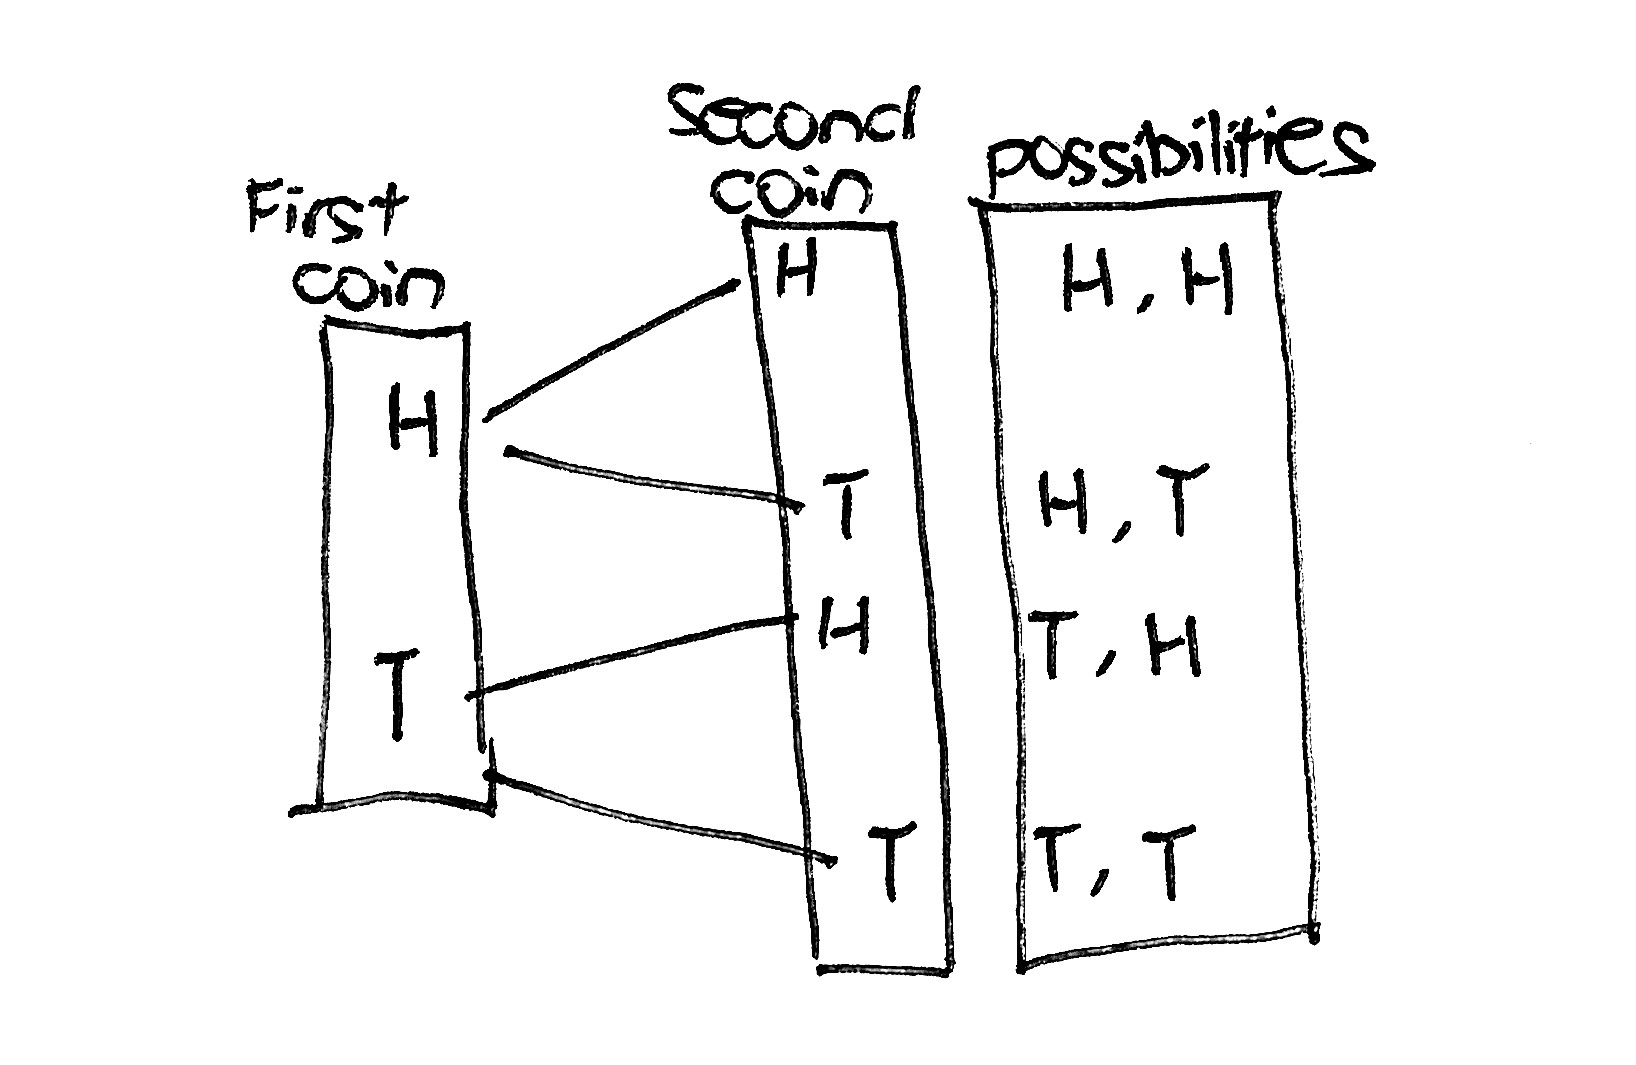
\includegraphics[width=0.43\textwidth]{./assets/prac1_1}
          \begin{flalign*}
            S = \left\{(H, H), (H, T), (T, H), (T, T)\right\}
          \end{flalign*}

    \item Write down the sample space of rolling a die once. \sol{}
          \begin{flalign*}
            S = \left\{1, 2, 3, 4, 5, 6\right\}
          \end{flalign*}

    \item Select any number from 0, 1, $\cdots$, 9, and write down its sample space.
          \sol{}
          \begin{flalign*}
            S = \left\{0, 1, 2, 3, 4, 5, 6, 7, 8, 9\right\}
          \end{flalign*}

    \item Write down the sample space of throwing a coin three times. \sol{}
          \begin{flalign*}
            S = & \left\{(H, H, H), (H, H, T), (H, T, H), (H, T, T),\right. & \\
                & \left.(T, H, H), (T, H, T), (T, T, H), (T, T, T)\right\}
          \end{flalign*}
  \end{enumerate}

  Within a trial, the set of a few sample points, that is, a subset of the sample
  space $S$, is called an \emph{event} of the trial, and is usually denoted by
  capital letters $A$, $B$, $C$, etc. The sample space $S$ in itself is also an
  event that will surely happen, and is called the \emph{sure event}. Empty set
  $\emptyset$ is also an event that will never happen, and is called the
  \emph{impossible event} or \emph{null event}. When an event only contains one
  sample point, that is, there is only one element of $S$ in the event, it is
  called a \emph{simple event}.

  For example, in the trial of throwing a dice for the dice points, the sure
  event $S = \{1, 2, 3, 4, 5, 6\}$, showing a dice points of 7 is an impossible
  event, and its denoted as $\emptyset$. The event of showing any of the dice
  points from 1 to 6 is a simple event.

  Take another example, draw a card from a deck of 52 poker cards, there are 52
  possible results. Hence, the sample space of this trial is a set of 52
  elements, and any event is a subset of the sample space. Below are some example
  of events in this sample space:

  \begin{enumerate}
    \item The card drawn is a number 11 (impossible event)
    \item The card drawn is a red heart 3 (simple event)
    \item The card drawn is a number 9 (event with 4 elements)
    \item The card drawn is a black spade (event with 13 elements)
    \item The card drawn is not a club 5 (event with 51 elements)
  \end{enumerate}

  Since the events are expressed as sets, listed below are some set operations
  used to describe relationships between events:

  Let $A$ and $B$ be two events, then:

  \begin{enumerate}
    \item $A \cup B$ means that at least one of the events $A$ and $B$ will happen.

    \item $A \cap B$ means that both events $A$ and $B$ will happen.

    \item $A'$ means that the event $A$ will not happen.
  \end{enumerate}

  \subsection{Practice 2}

  Express the following events in set notation (1 to 4):
  \begin{enumerate}
    \item Throwing a dice, event $A = $ "showing a prime number dice points". \sol{}
          \begin{flalign*}
            A = \left\{2, 3, 5\right\}
          \end{flalign*}

    \item Throwing three dices, event $B = $ "total dice points less than 6". \sol{}
          \begin{flalign*}
            B = & \left\{(1, 1, 1), (1, 1, 2), (1, 1, 3), (1, 2, 1),\right. \\
                & \left.(1, 2, 2), (1, 3, 1), (2, 1, 1), (2, 1, 2),\right.  \\
                & \left.(2, 2, 1), (3, 1, 1)\right\}
          \end{flalign*}

    \item Tossing two coins once, event $K = $ "showing exactly one head", event $L = $
          "showing at least one head", event $M = $ "showing at most one head". \sol{}

          Let $H$ and $T$ denote head and tail, respectively.
          \begin{flalign*}
            K & = \left\{(H, T), (T, H)\right\}         \\
            L & = \left\{(H, T), (T, H), (H, H)\right\} \\
            M & = \left\{(H, T), (T, H), (T, T)\right\}
          \end{flalign*}

    \item Tossing a coin three times:
          \begin{enumerate}
            \item $D = $ "get at least two heads".
                  \sol{}
                  \begin{flalign*}
                    D & = \left\{(T, H, H), (H, T, H), (H, H, T), (H, H, H)\right\} &
                  \end{flalign*}

            \item $E = $ "the number of heads is lesser than the number of tails".
                  \sol{}
                  \begin{flalign*}
                    E & = \left\{(H, T, T), (T, H, T), (T, T, H), (T, T, T)\right\} &
                  \end{flalign*}
          \end{enumerate}
  \end{enumerate}

  \subsection{Exercise 12.1}

  \begin{enumerate}
    \item Choose any two letters from the letters $K$, $O$, $T$, $A$, find:
          \begin{enumerate}
            \item The sample space $S$. \sol{}
                  \begin{flalign*}
                    S & = \left\{(K, O), (K, T), (K, A), (O, T), (O, A), (T, A)\right\} &
                  \end{flalign*}

            \item Event $A = $ "one letter is a vovel, the other is a consonant". \sol{}
                  \begin{flalign*}
                    A & = \left\{(K, O), (K, A), (O, T), (T, A)\right\} &
                  \end{flalign*}

            \item Event $B = $ "both letters are vovels".' \sol{}
                  \begin{flalign*}
                    B & = \left\{(O, A)\right\} &
                  \end{flalign*}

            \item Event $C = $ "at least one letter is a vovel". \sol{}
                  \begin{flalign*}
                    C & = \left\{(K, O), (K, A), (O, T), (O, A), (T, A)\right\} &
                  \end{flalign*}
          \end{enumerate}

    \item Throwing two dices, find the event where the sum of the dice points is a
          multiple of 3. \sol{}
          \begin{flalign*}
            S = & \left\{(1, 2), (2, 1), (3, 3), (4, 2), (2, 4), (5, 1), (1, 5),\right.   \\
                & \left. (6, 3), (3, 6), (4, 5), (5, 4), (6, 6)\right\}                 &
          \end{flalign*}

    \item Throwing three dices, find the event where the sum of the dice points is 15.
          \sol{}
          \begin{flalign*}
            S = & \left\{(6, 6, 3), (6, 3, 6), (3, 6, 6), (6, 5, 4), (6, 4, 5),\right.   \\
                & \left.(5, 6, 4), (5, 4, 6), (4, 6, 5), (4, 5, 6), (5, 5, 5)\right\}  &
          \end{flalign*}

    \item Choose any two letters from the letters $A$, $B$, $C$, $D$, $E$ to form a row,
          find:
          \begin{enumerate}
            \item The sample space $S$. \sol{}
                  \begin{flalign*}
                    S = & \left\{(A, B), (A, C), (A, D), (A, E), (B, A), (B, C),\right.   \\
                        & \left.(B, D), (B, E), (C, A), (C, B), (C, D), (C, E), \right.   \\
                        & \left.(D, A), (D, B), (D, C), (D, E), (E, A), (E, B), \right.   \\
                        & \left.(E, C), (E, D)\right\}                                  &
                  \end{flalign*}

            \item Event $M = $ "there are exactly one vowel". \sol{}
                  \begin{flalign*}
                    M = & \left\{(A, B), (A, C), (A, D), (B, A), (B, E), \right.   \\
                        & \left.(C, A), (C, E), (D, A), (D, E), (E, B), \right.    \\
                        & \left.(E, C), (E, D)\right\}                           &
                  \end{flalign*}
          \end{enumerate}

    \item Throwing three coins, find:
          \begin{enumerate}
            \item The sample space $S$. \sol{}
                  \begin{flalign*}
                    S = & \left\{(H, H, H), (H, H, T), (H, T, H), (H, T, T), \right.   \\
                        & \left.(T, H, H), (T, H, T), (T, T, H), (T, T, T)\right\}   &
                  \end{flalign*}

            \item Event $A = $ "all coins show heads". \sol{}
                  \begin{flalign*}
                    A = & \left\{(H, H, H)\right\} &
                  \end{flalign*}

            \item Event $B = $ "two coins show heads, one coin shows tail". \sol{}
                  \begin{flalign*}
                    B = & \left\{(H, H, T), (H, T, H), (T, H, H)\right\} &
                  \end{flalign*}

            \item Event $C = $ "at least two coin shows heads". \sol{}
                  \begin{flalign*}
                    C = & \left\{(H, H, H), (H, H, T), (H, T, H), (T, H, H)\right\} &
                  \end{flalign*}
          \end{enumerate}

    \item Throwing two dices, express the following events in set notation:
          \begin{enumerate}
            \item $A = $ "the dice points of two dices are equal".
                  \sol{}
                  \begin{flalign*}
                    A = & \left\{(1, 1), (2, 2), (3, 3), (4, 4), (5, 5), (6, 6)\right\} &
                  \end{flalign*}

            \item $B = $ "The dice points of one dice is twice the dice points of another".
                  \sol{}
                  \begin{flalign*}
                    B = & \left\{(1, 2), (2, 1), (3, 6), (6, 3)\right\} &
                  \end{flalign*}

            \item $C = $ "The sum of the dice points is a multiple of 5 or 6".
                  \sol{}
                  \begin{flalign*}
                    C = & \left\{(1, 4), (4, 1), (2, 3), (3, 2), (2, 4), (4, 2), (3, 3) \right. & \\
                        & \left.(5, 1), (1, 5), (6, 6), (6, 4), (4, 6), (5, 5) \right\}
                  \end{flalign*}
          \end{enumerate}
  \end{enumerate}

  \section{Definition of Probability}

  In this section, we'll cover two definitions of probability, the classical and
  the statistical definition.

  \subsection*{Statistical Definition of Probability}

  Doing a trial numerous times in the same conditions, the frequency of an event
  will show a certain regularity. Let's discuss the following example of
  dice-tossing:

  Tossing a dice multiple time and recording the numbers of time of getting 1
  dice point and the total number of tosses, we get the following results:

  \begin{center}
    \begin{tabular}{|c|c|c|}
      \hline
      Tosses ($n$) & No. of 1 dice points ($m$) & Frequency $\left(\frac{m}{n}\right)$ \\
      \hline
      1000         & 174                        & 0.1740                               \\
      2000         & 350                        & 0.1750                               \\
      3000         & 499                        & 0.1663                               \\
      4000         & 673                        & 0.1683                               \\
      5000         & 837                        & 0.1674                               \\
      6000         & 9999                       & 0.1665                               \\
      \hline
    \end{tabular}
  \end{center}

  From the table, we can see that as the number of tosses increases, the
  frequency of getting 1 dice point keep approaching a constant value of
  $\frac{1}{6} = 0.1667$.

  When performing a large amount of repeated trials, the frequency of an event
  $A$ $\left(\frac{m}{n}\right)$ always approaches a constant value. This
  constant value is called the \emph{probability} of event $A$, and denoted as
  $P(A)$. This is the statistical definition of probability.

  Since the occurrence of an event will never exceed the total number of trials,
  its frequency will always be a number between 0 and 1, that is, $0 \leq
    \frac{m}{n} \leq 1$. Hence, according to the statistical definition of
  probability, for any event $A$, its probability $0 \leq P(A) \leq 1$.

  A sure event $S$ will always happen in every trial, so $P(S) = 1$. For an
  impossible event $\emptyset$, no matter how many trials we do, its occurrence
  will always be 0, so $P(\emptyset) = 0$.

  \subsection*{Classical Definition of Probability}

  Assume that a trial satisfies the following conditions:

  \begin{enumerate}
    \item The outcome of the trial is finite.
    \item The probability of each outcome is equal.
  \end{enumerate}

  This kind of trial model is called a \emph{classical probabilistic model}.

  Let $S$ be the sample space of the trial that contains $n$ equally probable,
  $A$ is an event that contains $m$ outcomes, then the probability of event $A$
  is:
  \begin{cequation}
    P(A) = \frac{m}{n} = \frac{n(A)}{n(S)}
  \end{cequation}
  This is the classical definition of probability.

  \subsection{Practice 3}

  \begin{enumerate}
    \item Randomly draw two cards from a deck of 52 poker cards, find the probability of
          two "$K$" cards. \sol{}

          $S =$ "Randomly draw two cards from a deck of 52 poker
          cards", $n(S) = \comb[52]{2} = 1326$.

          Let event $A =$ "Two "$K$" cards", $n(A) = \comb[4]{2} = 6$.

          $P(A) = \frac{n(A)}{n(S)} = \frac{6}{1326} = \frac{1}{221}$.

    \item Between all students in a class, there are 13 students with type A blood, 10
          students with type B blood, 2 students with type AB blood, and 15 students with
          type O blood. If we randomly choose 4 students, find the probability of the
          following events: \sol{}

          $S =$ "Randomly choose 4 students", $n(S) = \comb[40]{4} = 91390$.
          \begin{enumerate}
            \item 2 type A blood, 2 type B blood
                  \sol{}

                  Let event $A =$ "2 type A blood, 2 type B blood", $n(A) = \comb[13]{2} \cdot
                    \comb[10]{2} = 3510$.

                  $P(A) = \frac{n(A)}{n(S)} = \frac{3510}{91390} = \frac{27}{703}$.

            \item 2 type A blood, 1 type AB blood, 1 type O blood
                  \sol{}

                  Let event $B =$ "2 type A blood, 1 type AB blood, 1 type O blood", $n(A) =
                    \comb[13]{2} \cdot \comb[2]{1} \cdot \comb[15]{1} = 2340$.

                  $P(B) = \frac{n(B)}{n(S)} = \frac{2340}{91390} = \frac{18}{703}$.

            \item 1 for each type of blood.
                  \sol{}

                  Let event $C =$ "1 for each type of blood", $n(C) = \comb[13]{1} \cdot
                    \comb[10]{1} \cdot \comb[2]{1} \cdot \comb[15]{1} = 3900$.

                  $P(C) = \frac{n(C)}{n(S)} = \frac{3900}{91390} = \frac{39}{703}$.
          \end{enumerate}

    \item Arranging all the letters in the word \textit{GERMANY}, find the probability of
          the following events: \sol{}

          $S =$ "Arranging all the letters in the word \textit{GERMANY}", $n(S) = 7!$.

          \begin{enumerate}
            \item 5 adjacent consonants
                  \sol{}

                  Let event $A =$ "5 adjacent consonants".

                  5 consonants can be treated as one letter, there are $3!$ ways to arrange 3 letters. All the consonants can switch their positions, so there are $5!$ ways to arrange 5 consonants.

                  $n(A) = 3! \cdot 5!$.

                  $P(A) = \frac{n(A)}{n(S)} = \frac{3! \cdot 5!}{7!} = \frac{1}{7}$.

            \item 5 non fully adjacent consonants
                  \sol{}

                  Let event $B =$ "5 non fully adjacent consonants".

                  $n(B) = n(S) - n(A) = 7! - 3! \cdot 5!$.

                  $P(B) = \frac{n(B)}{n(S)} = \frac{7! - 3! \cdot 5!}{7!} = \frac{6}{7}$.
          \end{enumerate}
  \end{enumerate}

  \subsection{Exerise 21.2}

  \begin{enumerate}
    \item A bag contains 9 balls, of which 2 are white, 3 are red, and 4 are yellow.
          Randomly drawing one ball, find the probability of the following events: \sol{}

          $S =$ "Randomly drawing one ball", $n(S) = \comb[9]{1}$.

          \begin{enumerate}
            \item The ball drawn is red \sol{}

                  Let event $A =$ "The ball drawn is red", $n(A) = \comb[3]{1}$.

                  $P(A) = \frac{n(A)}{n(S)} = \frac{\comb[3]{1}}{\comb[9]{1}} = \frac{1}{3}$.

            \item The ball drawn is not red \sol{}

                  Let event $B =$ "The ball drawn is not red", $n(B) = n(S) - n(A) = \comb[9]{1}
                    - \comb[3]{1}$.

                  $P(B) = \frac{n(B)}{n(S)} = \frac{\comb[9]{1} - \comb[3]{1}}{9} = \frac{2}{3}$.

            \item The ball drawn is yellow \sol{}

                  Let event $C =$ "The ball drawn is yellow", $n(C) = \comb[4]{1}$.

                  $P(C) = \frac{n(C)}{n(S)} = \frac{\comb[4]{1}}{\comb[9]{1}} = \frac{4}{9}$.
          \end{enumerate}

    \item A box contains 3 throat lozenges and 5 bubble gums. Randomly drawing two of
          them, find the probability of getting two bubble gums. \sol{}

          $S =$ "Randomly drawing two candies, $n(S) = \comb[8]{2}$.

          Let event $A =$ "Getting two bubble gums", $n(A) = \comb[5]{2}$.

          $P(A) = \frac{n(A)}{n(S)} = \frac{\comb[5]{2}}{\comb[8]{2}} = \frac{5}{14}$.

    \item Randomly drawing 3 cards from a deck of 52 poker cards, find the probability of
          getting 3 cards of spades. \sol{}

          $S =$ "Randomly drawing 3 cards from a deck of 52 poker cards", $n(S) = \comb[52]{3}$.

          Let event $A =$ "Getting 3 cards of spades", $n(A) = \comb[13]{3}$.

          $P(A) = \frac{n(A)}{n(S)} = \frac{\comb[13]{3}}{\comb[52]{3}} = \frac{11}{850}$.

    \item There are 4 novels and 8 essay collections in a box. Randomly drawing 3 books
          from the box, find the probability of the following events: \sol{}

          $S =$ "Randomly drawing 3 books from the box", $n(S) = \comb[12]{3}$.

          \begin{enumerate}
            \item All three books are novels \sol{}

                  Let event $A =$ "All three books are novels", $n(A) = \comb[4]{3}$.

                  $P(A) = \frac{n(A)}{n(S)} = \frac{\comb[4]{3}}{\comb[12]{3}} = \frac{1}{55}$.

            \item Two books of novels, one book of essay collection \sol{}

                  Let event $B =$ "Two books of novels, one book of essay collection", $n(B) =
                    \comb[4]{2} \cdot \comb[8]{1}$.

                  $P(B) = \frac{n(B)}{n(S)} = \frac{\comb[4]{2} \cdot \comb[8]{1}}{\comb[12]{3}} = \frac{12}{55}$.

            \item All three books are essay collections \sol{}

                  Let event $C =$ "All three books are essay collections", $n(C) = \comb[8]{3}$.

                  $P(C) = \frac{n(C)}{n(S)} = \frac{\comb[8]{3}}{\comb[12]{3}} = \frac{14}{55}$.
          \end{enumerate}

    \item A committee is to be formed by selecting 4 people from 6 males and 5 females.
          Find the probability of the following events: \sol{}

          Let event $S =$ "Selecting 4 people from 11 people", $n(S) = \comb[11]{4}$.

          \begin{enumerate}
            \item All 4 people are male \sol{}

                  Let event $A =$ "All 4 people are male", $n(A) = \comb[6]{4}$.

                  $P(A) = \frac{n(A)}{n(S)} = \frac{\comb[6]{4}}{\comb[11]{4}} = \frac{1}{22}$.

            \item All 4 people are female \sol{}

                  Let event $B = $ "All 4 people are female", $n(B) = \comb[5]{4}$.

                  $P(B) = \frac{n(B)}{n(S)} = \frac{\comb[5]{4}}{\comb[11]{4}} = \frac{1}{66}$.

            \item 2 people from each gender
                  \sol{}

                  Let event $C =$ "2 people from each gender", $n(C) = \comb[6]{2} \cdot
                    \comb[5]{2}$.

                  $P(C) = \frac{n(C)}{n(S)} = \frac{\comb[6]{2} \cdot \comb[5]{2}}{\comb[11]{4}} = \frac{5}{11}$.
          \end{enumerate}

    \item Of 100 products, 95 are quality products, and 5 are defective products.
          Randomly drawing 2 products, find the probability of the following events:
          \sol{}

          $S =$ "Randomly drawing 2 products", $n(S) = \comb[100]{2}$.

          \begin{enumerate}
            \item All 2 products are quality products \sol{}

                  Let event $A =$ "All 2 products are quality products", $n(A) = \comb[95]{2}$.

                  $P(A) = \frac{n(A)}{n(S)} = \frac{\comb[95]{2}}{\comb[100]{2}} = \frac{893}{990}$.

            \item All 2 products are defective products \sol{}

                  Let event $B =$ "All 2 products are defective products", $n(B) = \comb[5]{2}$.

                  $P(B) = \frac{n(B)}{n(S)} = \frac{\comb[5]{2}}{\comb[100]{2}} = \frac{1}{495}$.

            \item 1 quality products, 1 defective product
                  \sol{}

                  Let event $C =$ "1 quality products, 1 defective product", $n(C) = \comb[95]{1}
                    \cdot \comb[5]{1}$.

                  $P(C) = \frac{n(C)}{n(S)} = \frac{\comb[95]{1} \cdot \comb[5]{1}}{\comb[100]{2}} = \frac{19}{198}$.
          \end{enumerate}

    \item Randomly choose 3 letters from the word \textit{TRIANGLE}, find the probability
          of the following events: \sol{}

          $S =$ "Randomly choose 3 letters from the word \textit{TRIANGLE}", $n(S) = \comb[8]{3}$.

          \begin{enumerate}
            \item More vowels than consonants \sol{}

                  Let event $A =$ "More vowels than consonants".

                  Choose three vowels from the word \textit{TRIANGLE}, there are $\comb[3]{3}$
                  ways to do so.

                  Choose two vowels and one consonant from the word \textit{TRIANGLE}, there are
                  $\comb[3]{2} \cdot \comb[5]{1}$ ways to do so.

                  $n(A) = \comb[3]{3} + \comb[3]{2} \cdot \comb[5]{1}$.

                  $P(A) = \frac{n(A)}{n(S)} = \frac{\comb[3]{3} + \comb[3]{2} \cdot \comb[5]{1}}{\comb[8]{3}} = \frac{2}{7}$.

            \item More consonants than vowels \sol{}

                  Let event $B =$ "More consonants than vowels".

                  Choose three consonants from the word \textit{TRIANGLE}, there are
                  $\comb[5]{3}$ ways to do so.

                  Choose two consonants and one vowel from the word \textit{TRIANGLE}, there are
                  $\comb[5]{2} \cdot \comb[3]{1}$ ways to do so.

                  $n(B) = \comb[5]{3} + \comb[5]{2} \cdot \comb[3]{1}$.

                  $P(B) = \frac{n(B)}{n(S)} = \frac{\comb[5]{3} + \comb[5]{2} \cdot \comb[3]{1}}{\comb[8]{3}} = \frac{5}{7}$.
          \end{enumerate}

    \item Tossing three dices at the same time once, find the probability of the sum of
          dice points larger than 15. \sol{}

          $S =$ "Tossing three dices at the same time once", $n(S) = 6^3 = 216$.

          Let event $A =$ "The sum of dice points larger than 15".

          $A = \{ (6, 6, 6), (6, 6, 5), (6, 5, 6), (6, 6, 5), (6, 6, 4), (6, 4, 6), $
          $(4, 6, 6), (6, 5, 5), (5, 6, 5), (5, 5, 6)\}$.

          $n(A) = 10$.

          $P(A) = \frac{n(A)}{n(S)} = \frac{10}{216} = \frac{5}{108}$.

    \item Randomly shuffling each digits in 2233344455, find the probability of two 2s
          being adjacent to each other.

          \sol{}

          $S =$ "Randomly shuffling each digits in 2233344455", $n(S) = \frac{10!}{2! \cdot 3! \cdot 3! \cdot 2!} = 25200$.

          Let event $A =$ "Two 2s being adjacent to each other".

          Treat two 2s as a single 2, there are $\frac{9!}{1! \cdot 3! \cdot 3! \cdot 2!}
            = 5040$ ways to do so.

          $n(A) = 5040$.

          $P(A) = \frac{n(A)}{n(S)} = \frac{5040}{25200} = \frac{1}{5}$.

    \item Randomly shuffling 5 cards that are assigned to 1, 2, 3, 4, 5 respectively and
          arranging them into a 5 digit number, find the probability of the number being
          an even number.

          \sol{}

          $S =$ "Randomly shuffling 5 cards that are assigned to 1, 2, 3, 4, 5 respectively"

          $n(S) = 5!$.

          Let event $A =$ "The number being an even number".

          Since the number is even, the last digit must be 2 or 4. There are $2$ ways to
          arrange it. For the other 4 digits, there are $4!$ ways to do arrange them.

          $n(A) = 2 \cdot 4!$.

          $P(A) = \frac{n(A)}{n(S)} = \frac{2 \cdot 4!}{5!} = \frac{2}{5}$.
  \end{enumerate}

  \section{Addition Rule}

  \subsection*{Mutually Exclusive Events and Inclusive Events}

  When two events $A$ and $B$ can happen at the same time, event $A$ and $B$ are
  said to be \emph{inclusive}. For example, when tossing a dice once, the events
  "getting an even number" and "getting a multiple of 3" can happen at the same
  time. Therefore, these two events are inclusive events. Now let's find the
  probability of getting an even number or a multiple of 3 when tossing a dice
  once.

  \noindent Let the sample space of the trial be $S = \{1, 2, 3, 4, 5, 6\},\ n(S) = 6$.

  \noindent Let event $A = $ "getting an even number" $ = \{2, 4, 6\},\ n(A) = 3$, therefore $P(A) = \frac{3}{6}$.

  \noindent Let event $B = $ "getting a multiple of 3" $ = \{3, 6\},\ n(B) = 2$, therefore $P(B) = \frac{2}{6}$.

  \noindent $A \cup B = $ "getting an even number or a multiple of 3" $ = \{2, 3, 4, 6\},\ n(A \cup B) = 4$, therefore $P(A \cup B) = \frac{4}{6} = \frac{2}{3}$.

  \noindent $A \cap B = $ "getting an even number that is also a multiple of 3" $ = \{6\},\ n(A \cap B) = 1$, therefore $P(A \cap B) = \frac{1}{6}$.

  \noindent Generally speaking, according to the formula of cardinality of the union of two sets,
  \begin{cequation}
    n(A \cup B) = n(A) + n(B) - n(A \cap B)
  \end{cequation}
  Dividing both side by $n(S)$, we get:
  \begin{cequation}
    \frac{n(A \cup B)}{n(S)} = \frac{n(A)}{n(S)} + \frac{n(B)}{n(S)} - \frac{n(A \cap B)}{n(S)}
  \end{cequation}
  That is,
  \begin{cequation}
    P(A \cup B) = P(A) + P(B) - P(A \cap B)
  \end{cequation}

  The relationship is the \emph{addition rule} of probability.

  In the example above,
  \begin{flalign*}
    P(A \cup B) & = P(A) + P(B) - P(A \cap B)               \\
                & = \frac{3}{6} + \frac{2}{6} - \frac{1}{6} \\
                & = \frac{2}{3}
  \end{flalign*}

  When two events $A$ and $B$ cannot happen at the same time, that is, $A \cap B
    = \emptyset$, $A$ and $B$ is said to be mutually exclusive. For example, there
  are a red ball and a white ball in a bag. When randomly drawing one ball, the
  ball will be either red or white, but not both. This is a mutually exclusive
  event.

  Since $A$ and $B$ are mutually exclusive, $P(A \cap B) = 0$.
  \begin{cequation}
    P(A \cup B) = P(A) + P(B)
  \end{cequation}

  The relationship above is the additional rule of mutually exclusive events.

  From that, we know that if event $A$ and event $B$ are mutually exclusive,
  their probability is the sum of their individual probabilities.

  \subsection{Practice 4}

  \begin{enumerate}
    \item A bag contains 5 cards each for the color red, blue and green. Randomly drawing
          one card, find the probability of getting a red card or a yellow card. \sol{}

          Let event $A =$ "getting a red card", $P(A) = \frac{5}{15}$.

          Let event $B =$ "getting a yellow card", $P(B) = \frac{5}{15}$.

          $A \cup B =$ "getting a red card or a yellow card".

          Since $A$ and $B$ are mutually exclusive,
          \begin{flalign*}
            \therefore\ P(A \cup B) & = P(A) + P(B)                   \\
                                    & = \frac{5}{15} + \frac{5}{15} & \\
                                    & = \frac{10}{15}                 \\
                                    & = \frac{2}{3}
          \end{flalign*}

    \item Drawing a card from a deck of 52 poker cards, find the probability of getting a
          heart or number that is a multiple of 5. \sol{}

          Let event $A =$ "getting a heart", $P(A) = \frac{13}{52}$.

          Let event $B =$ "getting a number that is a multiple of 5", $P(B) =
            \frac{8}{52}$.

          $A \cup B =$ "getting a heart or a number that is a multiple of 5".

          $A \cap B =$ "getting a heart that is also a number that is a multiple of 5", $P(A \cap B) = \frac{2}{52}$.
          \begin{flalign*}
            \therefore\ P(A \cup B) & = P(A) + P(B) - P(A \cap B)                   & \\
                                    & = \frac{13}{52} + \frac{8}{52} - \frac{2}{52}   \\
                                    & = \frac{19}{52}
          \end{flalign*}

    \item Of a class of 45 students, 20 of them has visited Bali or Jakarta, of which 14
          of them has visited Bali and 10 of them has visited Jakarta. Randomly choosing
          one student, find the probability of the student has visited both cities.
          \sol{}

          Let event $A =$ "visited Bali", $P(A) = \frac{14}{45}$.

          Let event $B =$ "visited Jakarta", $P(B) = \frac{10}{45}$.

          $A \cup B =$ "visited Bali or Jakarta", $P(A \cup B) = \frac{20}{45}$.

          $A \cap B =$ "visited Bali and Jakarta".
          \begin{flalign*}
            P(A \cup B)             & = P(A) + P(B) - P(A \cap B)                     & \\
            \therefore\ P(A \cap B) & = P(A \cup B) - P(A) - P(B)                       \\
                                    & = \frac{20}{45} - \frac{14}{45} - \frac{10}{45}   \\
                                    & = \frac{4}{45}
          \end{flalign*}
  \end{enumerate}

  \subsection*{Complementary Events}

  During a trial, if one of two mutually exclusive events $A$ and $B$ must
  happen, then these two events are said to be complementary events. The
  complementary event of an event $A$ is denoted by $A'$. Take coin-tossing as an
  example, if event $A$ is "getting a head", then its complementary event $A'$ is
  "getting a tail". Since either event $A$ or $A'$ must happen, therefore $A \cup
    A' = S$. Applying additional rule for mutually exclusive events, \makeatletter
  \setbool{@fleqn}{false} \makeatother
  \begin{flalign*}
    P(A) + P(A')     & = P(A \cup A') \\
                     & = P(S)         \\
                     & = 1            \\
    \therefore\ P(A) & = 1 - P(A')
  \end{flalign*}
  \makeatletter
  \setbool{@fleqn}{true}
  \makeatother

  The relationship above can be used to calculat the probability of complementary
  events.

  \subsection{Practice 5}

  \begin{enumerate}
    \item There are 22 boys and 23 girls in a class. Randomly picking 2 students from
          them, find the probability of having at least one boy in these 2 people. \sol{}

          $S =$ "picking 2 students from the class".

          $n(S) = \comb[45]{2} = 990$.

          Let event $A =$ "Having at least one boy in these 2 people",

          then $A' = $ "All people are girls".

          $n(A') = \comb[23]{2} = 253$. $P(A') = \frac{23}{90}$.
          \begin{flalign*}
            \therefore\ P(A) & = 1 - P(A')         & \\
                             & = 1 - \frac{23}{90}   \\
                             & = \frac{67}{90}
          \end{flalign*}

    \item In a lucky draw, there are 60 boxes, of which 5 of them contain a prize.
          Randomly picking 2 boxes, find the probability of getting at least one prize.
          \sol{}

          $S =$ "picking 2 boxes from the lucky draw".

          $n(S) = \comb[60]{2} = 1770$.

          Let event $A =$ "Getting at least one prize",

          then $A' = $ "Getting no prize".

          $n(A') = \comb[55]{2} = 1485$. $P(A') = \frac{99}{118}$.
          \begin{flalign*}
            \therefore\ P(A) & = 1 - P(A')          & \\
                             & = 1 - \frac{99}{118}   \\
                             & = \frac{19}{118}
          \end{flalign*}
  \end{enumerate}

  \subsection{Exercise 21.3}

  \begin{enumerate}
    \item There are 5 red balls, 6 yellow balls, and 8 black balls in a box. Randomly
          drawing one ball, find the probability of getting a red ball or a yellow ball.
          \sol{}

          Let event $A =$ "getting a red ball", $P(A) = \frac{5}{19}$.

          Let event $B =$ "getting a yellow ball", $P(B) = \frac{6}{19}$.

          $A \cup B =$ "getting a red ball or a yellow ball".

          Since $A$ and $B$ are mutually exclusive events,
          \begin{flalign*}
            P(A \cup B) & = P(A) + P(B)                 & \\
                        & = \frac{5}{19} + \frac{6}{19}   \\
                        & = \frac{11}{19}
          \end{flalign*}

    \item There are 18 different reference books on the shelf, of which 6 of them are
          Chinese and 5 of them are Maths, and the rest of them are Ecomoics. Randomly
          picking two books from the shelf, find the probability of getting at least one
          Math book or one Chinese book. \sol{}

          $S =$ "picking two books from the shelf".

          $n(S) = \comb[18]{2} = 153$.

          Let event $A =$ "getting one Math book or one Chinese book",

          then $A' = $ "all two books are Economics books".

          $n(A') = \comb[7]{2} = 21$. $P(A') = \frac{21}{153}$.
          \begin{flalign*}
            \therefore\ P(A) & = 1 - P(A')          & \\
                             & = 1 - \frac{21}{153}   \\
                             & = \frac{44}{153}
          \end{flalign*}

    \item There are 15 shirts, 10 vests and 5 T-shirts on the rack. Randomly picking two
          clothes from the rack, find the probability of getting at least one T-shirt.
          \sol{}

          $S =$ "picking two clothes from the rack".

          $n(S) = \comb[30]{2} = 435$.

          Let event $A =$ "getting at least one T-shirt",

          then $A' = $ "getting no T-shirt".

          $n(A') = \comb[25]{2} = 300$. $P(A') = \frac{20}{29}$.
          \begin{flalign*}
            \therefore\ P(A) & = 1 - P(A')         & \\
                             & = 1 - \frac{20}{29}   \\
                             & = \frac{9}{29}
          \end{flalign*}

    \item There are 50 prizes in a lucky draw, of which 1 of them is cash prize worth
          \$800, 2 of them are cash prize worth \$500, 5 of them are cash prize worth
          \$100, and the rest of them are bookshop vouchers worth \$10. One person make
          two draws, find the probability of getting at least one cash prize. \sol{}

          $S =$ "making two draws".

          $n(S) = \comb[50]{2} = 1225$.

          Let event $A =$ "getting at least one cash prize",

          then $A' = $ "getting no cash prize".

          $n(A') = \comb[42]{2} = 861$. $P(A') = \frac{123}{175}$.
          \begin{flalign*}
            \therefore\ P(A) & = 1 - P(A')           & \\
                             & = 1 - \frac{123}{175}   \\
                             & = \frac{52}{175}
          \end{flalign*}

    \item There are 50 people doing a meeting in a classroom, of which 35 of them are
          students, 12 of them are parents, and 3 of them are teachers. Randomly picking
          one spokesperson, find the probability of the following events:
          \begin{enumerate}
            \item The spokesperson is either a teacher or a student. \sol{}

                  Let event $A =$ "the spokesperson is a teacher", $P(A) = \frac{3}{50}$.

                  Let event $B =$ "the spokesperson is a student", $P(B) = \frac{35}{50}$.

                  $A \cup B =$ "the spokesperson is either a teacher or a student".

                  Since $A$ and $B$ are mutually exclusive events,
                  \begin{flalign*}
                    P(A \cup B) & = P(A) + P(B)                  & \\
                                & = \frac{3}{50} + \frac{35}{50}   \\
                                & = \frac{19}{25}
                  \end{flalign*}

            \item The spokesperson is either a teacher or a parent. \sol{}

                  Let event $A =$ "the spokesperson is a teacher", $P(A) = \frac{3}{50}$.

                  Let event $B =$ "the spokesperson is a parent", $P(B) = \frac{12}{50}$.

                  $A \cup B =$ "the spokesperson is either a teacher or a parent".

                  Since $A$ and $B$ are mutually exclusive events,
                  \begin{flalign*}
                    P(A \cup B) & = P(A) + P(B)                  & \\
                                & = \frac{3}{50} + \frac{12}{50}   \\
                                & = \frac{3}{10}
                  \end{flalign*}

            \item The spokesperson is either a student or a parent. \sol{}

                  Let event $A =$ "the spokesperson is a student", $P(A) = \frac{35}{50}$.

                  Let event $B =$ "the spokesperson is a parent", $P(B) = \frac{12}{50}$.

                  $A \cup B =$ "the spokesperson is either a student or a parent".

                  Since $A$ and $B$ are mutually exclusive events,
                  \begin{flalign*}
                    P(A \cup B) & = P(A) + P(B)                   & \\
                                & = \frac{35}{50} + \frac{12}{50}   \\
                                & = \frac{47}{50}
                  \end{flalign*}
          \end{enumerate}

    \item There are 100 lottery tickets, of which 3 of them are winning tickets. One
          person has bought 10 tickets, find the probability of the following events:
          \begin{enumerate}
            \item All tickets are not winning tickets. \sol{}

                  $S=$ "bought 10 tickets". $n(S) = \comb[100]{10}$.

                  Let event $A =$ "all tickets are not winning tickets". $n(A) = \comb[97]{10}$.

                  $P(A) = \frac{n(A)}{n(S)} = \frac{\comb[97]{10}}{\comb[100]{10}} = \frac{178}{245}$.

            \item At least one ticket is a winning ticket. \sol{}

                  Let event $B =$ "at least one ticket is a winning ticket",

                  then $B' = $ "all tickets are not winning tickets".
                  \begin{flalign*}
                    P(B) & = 1 - P(B')           & \\
                         & = 1 - \frac{178}{245}   \\
                         & = \frac{67}{245}
                  \end{flalign*}
          \end{enumerate}

    \item There are 11 out of 45 students in a class who have donated their blood before.
          Randomly picking three students, find the probability of the following events:
          \begin{enumerate}
            \item All three students have donated their blood before. \sol{}

                  $S =$ "picking three students". $n(S) = \comb[45]{3}$.

                  Let event $A =$ "all three students have donated their blood before".

                  $n(A) = \comb[11]{3}$.

                  $P(A) = \frac{n(A)}{n(S)} = \frac{\comb[11]{3}}{\comb[45]{3}} = \frac{1}{86}$.

            \item All three students have never donated their blood before. \sol{}

                  Let $B =$ "all three students have never donated their blood before".

                  $n(B) = \comb[34]{3}$.

                  $P(B) = \frac{n(B)}{n(S)} = \frac{\comb[34]{3}}{\comb[45]{3}} = \frac{272}{645}$.

            \item At least one student has donated his/her blood before. \sol{}

                  Let $C =$ "at least one student has donated his/her blood before",

                  then $C' =$ "all three students have never donated their blood before".
                  \begin{flalign*}
                    P(C) & = 1 - P(C')           & \\
                         & = 1 - \frac{272}{645}   \\
                         & = \frac{373}{645}
                  \end{flalign*}
          \end{enumerate}

    \item Tossing two dices at the same time, find the probability of the sum of the dice
          points being at least 9. \sol{}

          $S =$ "tossing two dices". $n(S) = 6^2 = 36$.

          Let event $A =$ "the sum of the dice points is at least 9".

          $A = \{(3, 6), (4, 5), (5, 4), (6, 3), (5, 5), (6, 4), (4, 6), (6, 5), $
          $(5, 6), (6, 6)\}$.

          $n(A) = 10$.

          $P(A) = \frac{n(A)}{n(S)} = \frac{10}{36} = \frac{5}{18}$.

    \item Continuously tossing a coin 5 times, find the probability of getting at least
          one head.\sol{}

          $S =$ "tossing a coin 5 times". $n(S) = 2^5 = 32$.

          Let event $A =$ "getting at least one head",

          then $A' =$ "getting no head".

          $A' = \{(T, T, T, T, T)\}$.

          $n(A') = 1$.

          $P(A) = 1 - P(A') = 1 - \frac{1}{32} = \frac{31}{32}$.

    \item There are 7 red balls and 10 white balls in a box. Randomly drawing 3 balls,
          find the probability of the following events: \sol{}

          $S =$ "drawing 3 balls". $n(S) = \comb[17]{3}$.

          \begin{enumerate}
            \item Getting at least one red ball. \sol{}

                  Let event $A =$ "getting at least one red ball",

                  then $A' =$ "getting all white ball". $n(A') = \comb[10]{3}$. $P(A') =
                    \frac{n(A')}{n(S)} = \frac{\comb[10]{3}}{\comb[17]{3}} = \frac{3}{17}$.
                  \begin{flalign*}
                    P(A) & = 1 - P(A')        & \\
                         & = 1 - \frac{3}{17}   \\
                         & = \frac{14}{17}
                  \end{flalign*}

            \item Getting at least one white ball. \sol{}

                  Let event $B =$ "getting at least one white ball",

                  then $B' =$ "getting all red ball". $n(B') = \comb[7]{3}$. $P(B') =
                    \frac{n(B')}{n(S)} = \frac{\comb[7]{3}}{\comb[17]{3}} = \frac{7}{136}$.
                  \begin{flalign*}
                    P(B) & = 1 - P(B')         & \\
                         & = 1 - \frac{7}{136}   \\
                         & = \frac{129}{136}
                  \end{flalign*}

            \item Getting at least two red balls. \sol{}

                  Let event $C =$ "getting at least two red balls",

                  then $C' =$ "getting no red ball or only one red ball".

                  Let event $D =$ "getting no red ball",

                  then $D' =$ "getting at least one red ball" $=A$.
                  \begin{flalign*}
                    P(D) & = 1 - P(A)          & \\
                         & = 1 - \frac{14}{17}   \\
                         & = \frac{3}{17}
                  \end{flalign*}

                  Let event $E =$ "getting only one red ball", $n(E) = \comb[7]{1} \cdot
                    \comb[10]{2}$.

                  $P(E) = \frac{n(E)}{n(S)} = \frac{\comb[7]{1} \cdot \comb[10]{2}}{\comb[17]{3}} = \frac{63}{136}$.

                  Since event $E$ and event $D$ are mutually exclusive,
                  \begin{flalign*}
                    P(C')            & = P(D) + P(E)                   & \\
                                     & = \frac{3}{17} + \frac{63}{136}   \\
                                     & = \frac{87}{136}                  \\
                    \therefore\ P(C) & = 1 - P(C')                     & \\
                                     & = 1 - \frac{87}{136}              \\
                                     & = \frac{49}{136}
                  \end{flalign*}

          \end{enumerate}

    \item Tossing 3 dices once, find the probabily of hte following events: \sol{}

          $S =$ "tossing 3 dices". $n(S) = 6^3 = 216$.

          \begin{enumerate}
            \item Exactly one dice shows 6. \sol{}

                  Let event $A =$ "exactly one dice shows 6".

                  There are $\comb[3]{1} = 3$ outcomes for one dice to shows 6. The other two
                  dices show 1, 2, 3, 4, or 5, there are $5^2$ outcomes. The total number of
                  outcomes is $3 5^2 \cdot = 75$.

                  $P(A) = \frac{n(A)}{n(S)} = \frac{75}{216} = \frac{25}{72}$.

            \item Exactly one dice or all three dices show 1. \sol{}

                  Let event $B =$ "exactly one dice shows 1".

                  There are $\comb[3]{1} = 3$ outcomes for one dice to shows 1. The other two
                  dices show 2, 3, 4, 5, or 6, there are $5^2$ outcomes. The total number of
                  outcomes is $3 5^2 = 75$.

                  $P(B) = \frac{n(B)}{n(S)} = \frac{75}{216} = \frac{25}{72}$.

                  Let event $C =$ "all three dices show 1". $n(C) = 1$.

                  $P(C) = \frac{n(C)}{n(S)} = \frac{1}{216}$.

                  Since event $B$ and event $C$ are mutually exclusive,
                  \begin{flalign*}
                    P(B \cup C) & = P(B) + P(C)                   & \\
                                & = \frac{25}{72} + \frac{1}{216}   \\
                                & = \frac{19}{54}
                  \end{flalign*}
          \end{enumerate}
  \end{enumerate}

  \section{Multiplication Rule}

  \subsection*{Independent Events}

  For two events $A$ and $B$, if the occurrence of event $A$ does not affect the
  occurrence of event $B$, then the two events are said to be independent events.
  For example, tossing a dice twice, the result of the first toss does not affect
  the result of the second toss, vice versa. Therefore, the two events are
  independent events. The probability of the two events occurring is the product
  of their individual probabilities:
  \begin{cequation}
    P(A \cap B) = P(A) \cdot P(B)
  \end{cequation}

  \subsection{Practice 6}

  \begin{enumerate}
    \item There are 10 oranges and 12 apples in two baskets respectively, of which 2
          oranges and 4 apples are rotten. Randomly picking one fruit from each basket,
          find the probability of getting two rotten fruits. \sol{}

          The probability of getting a rotten orange is $\frac{2}{10} = \frac{1}{5}$.

          The probability of getting a rotten apple is $\frac{4}{12} = \frac{1}{3}$.

          Therefore, the probability of getting two rotten fruits is $\frac{1}{5} \cdot
            \frac{1}{3} = \frac{1}{15}$.

    \item Person $A$ and person $B$ are participating in a archery competition. Person
          $A$ and person $B$ have a probability of $\frac{5}{8}$ and $\frac{7}{15}$
          respectively to hit the bullseye. Find the probability the following events:
          \begin{enumerate}
            \item Both person $A$ and person $B$ hit the bullseye. \sol{}

                  Let the event of person $A$ and person $B$ both hitting the bullseye be $A$.
                  \begin{flalign*}
                    P(A) & = \frac{5}{8} \cdot \frac{7}{15} \\
                         & = \frac{7}{24}
                  \end{flalign*}

            \item Both of them does not hit the bullseye. \sol{}

                  Let the event of person $A$ not hitting the bullseye be $B$, then $B'$ is the
                  event of person $A$ hitting the bullseye.

                  Let the event of person $B$ not hitting the bullseye be $C$, then $C'$ is the
                  event of person $B$ hitting the bullseye.
                  \begin{flalign*}
                    P(B \cap C) & = P(B) \cdot P(C)                        \\
                                & = 1 - P(B') \cdot 1 - P(C')              \\
                                & = 1 - \frac{5}{8} \cdot 1 - \frac{7}{15} \\
                                & = \frac{3}{8} \cdot \frac{8}{15}         \\
                                & = \frac{1}{5}
                  \end{flalign*}

            \item At least one of them hits the bullseye. \sol{}

                  Let the event of at least one of them hits the bullseye be $D$, then $D'$ is
                  the event of both of them not hitting the bullseye.
                  \begin{flalign*}
                    P(D) & = 1 - P(D')       \\
                         & = 1 - \frac{1}{5} \\
                         & = \frac{4}{5}
                  \end{flalign*}
          \end{enumerate}
  \end{enumerate}

  \subsection{Exercise 21.4a}

  \begin{enumerate}
    \item Tossing a dice three times, find the probability of getting 2 for the first and
          the second toss, and an odd number for the third toss.

    \item Tossing a coin 5 times, find the probability of getting at 4 heads
          continuously.

    \item The forecast accuracy of a weather station is 80\%. Find probability of getting
          4 accurate forecasts our of 5 forecasts. (Round to the nearest 4 decimal
          places)

    \item There are three processes for processing a component, the failure rate of each
          process are $1.2\%$, $1.8\%$, and $0.8\%$ respectively. If the chance of
          failure of the component does not depend on other processes, find the success
          rate of the component.

    \item Randomly drawing 1 card from a deck of 52 cards, and draw another card without
          putting the first card back into the deck. Find the probability of getting a
          spade for the second card.

    \item 3 people are decrypting a message on their own. The probability of each of them decrypting the message correctly is $\frac{1}{5}$, $\frac{1}{4}$ and $\frac{1}{3}$ respectively. Find the probability the message getting decrypted.

    \item 3 people are participating in an archery competition. person $A$ make three hits out of five, person $B$ make two hits out of three, person $C$ make one hit out of two. Now each person gets one shot, find the probability of the following events:
          \begin{enumerate}
            \item All three of them make a hit.
            \item Only one of them make a hit.
            \item At least one of them make a hit.
          \end{enumerate}

    \item There are 5 black balls, 4 yellow balls, and 3 white balls in a box. Randomly
          draw one balls and put it back into the box. Repeat the process 3 times. Find
          the probability of the following events:
          \begin{enumerate}
            \item Only get one yellow ball
            \item All three balls are yellow balls
            \item Get one black ball, one yellow ball, and one white ball
          \end{enumerate}
  \end{enumerate}

  \subsection{Practice 7}

  There are $80\%$ of the families living in a town have signed up for fibre
  optic cable. Now choose 10 random families from the town for a survey, find the
  probability of the following events (round to the nearest 4 decimal places):

  \begin{enumerate}
    \item Exactly half of the families have signed up for fibre optic cable.

    \item All of the families have signed up for fibre optic cable.

    \item At least one family has not signed up for fibre optic cable.
  \end{enumerate}

  \subsection{Exercise 21.4b}

  \begin{enumerate}
    \item The survival rate of a plant is $0.6$. Now 10 plants are planted, find the
          probability exactly 5 of them survive.

    \item The hit rate of a person shooting a basket ball is $0.4$. Find the probability
          of him making 10 hit out of 25 shots.

    \item According to statistical data, there are $85\%$ of the population in a city has
          Hepatitis B Vaccination. Now randomly choose 8 people from the city for a
          health check, find the probability of at most two of them have not been
          vaccinated.

    \item The probability of a medicine successfully curing a cold is $0.96$. Now 10 cold
          patients are taking the medicine, find the probability of at least 8 of them
          are cured.

    \item A factory produces a component, the probability of the component being
          defective is $0.04$. Now 20 components are produced, find the probability of
          the following events:
          \begin{enumerate}
            \item Exactly 1 of them is defective.
            \item Exactly 2 of them are defective.
            \item At most one of them is defective.
          \end{enumerate}

    \item Tossing a coin 5 times, find the probability of the following events:
          \begin{enumerate}
            \item Exactly 3 heads.
            \item At least 3 heads.
            \item The number of heads is odd.
          \end{enumerate}

    \item A person will4 four traffic lights on his way to work. Given that the duration
          of red, yellow, and green lights are $90s$, $5s$ and $25s$ respectively for
          each light. Find the probability of the following events:
          \begin{enumerate}
            \item Get a red light for the every light.
            \item Only get a red light for the first two lights.
            \item Get exactly two red lights.
          \end{enumerate}
  \end{enumerate}

  \section{Mathematical Expectation}

  Consider the following scenario: during a commercial activity, the probability
  of a person getting a profit of \$300 is $0.6$, and the probability of a person
  getting a loss of \$100 is $0.4$. He did the activity 10 times. According to
  the probability, this guy was expected to get a profit of \$300 for 6 times,
  and a loss of \$100 for 4 times. Therefore, the expected profit of these 10
  times of commercial activities is $300 \cdot 6 + (-100) \cdot 4$.
  \begin{flalign*}
    \text{Average Profit} & = \frac{300 \cdot 6 + (-100) \cdot 4}{10} \\
                          & = \frac{1800 - 400}{10}                   \\
                          & = \frac{1400}{10}                         \\
                          & = 140
  \end{flalign*}
  This average value is called the \textit{mathematical expectated value}, or \textit{expected value} for short, of this people doing the commercial activity.

  The expect value does not mean that the actual profit of the person will be
  \$140 for every activity he did. It is just the average value of the profit he
  will get if he did the activity a large number of times.

  Generalize the above example, let the probability of someone getting a profit
  of $\$x_1$, $\$x_2$, $\cdots$, $\$x_k$ be $p_1$, $p_2$, $\cdots$, $p_k$
  respectively, of which $p_1 + p_2 + \cdots + p_k = 1$. Then the expected value
  of the profit is
  \begin{cequation}
    E = x_1p_1 + x_2p_2 + \cdots + x_kp_k
  \end{cequation}

  \subsection{Practice 8}

  \begin{enumerate}
    \item One person pays \$2 to play a a game. The chance of winning the game is $0.4$,
          and he will get \$3 if he wins. Find the expected value of profit of this
          person in this game. \sol{}

          \noindent The chance of winning the game is $0.4$, and the profit of winning the game is
          \$1;

          \noindent The chance of losing the game is $0.6$, and the loss of losing the game is \$2.

          Therefore, the expected value of profit of this person in this game is
          \begin{flalign*}
            E & = 0.4 \cdot 1 + 0.6 \cdot (-2) \\
              & = 0.4 - 1.2                    \\
              & = -\$0.80
          \end{flalign*}

    \item During an investment activity, the probability of a person getting a profit of
          \$2,500 is $0.55$, and the probability of a person getting a loss of \$1,200 is
          $0.45$. Find the expected value of profit of this person in this investment
          activity. \sol{}

          The expected value of profit of this person in this investment activity is
          \begin{flalign*}
            E & = 2500 \cdot 0.55 + (-1200) \cdot 0.45 \\
              & = 1375 - 540                           \\
              & = \$835
          \end{flalign*}
  \end{enumerate}

  \subsection{Exercise 21.5}

  \begin{enumerate}
    \item During a commercial activity, the probability of a person getting a profit of
          $\$10,000$ is $\frac{3}{5}$, and the probability of a person getting a loss of
          $\$6,000$ is $\frac{2}{5}$. Find the expected value of profit of this person in
          this commercial activity.

    \item A company produces light bulbs. The profit of producing a quality light bulb is
          $\$2$, and the loss of producing a defective light bulb is $\$0.50$. Assume
          that the chance of producing a defective light bulb is $0.02$. Find the
          expected value of profit of this company in producing each light bulb.

    \item A company has insured accident insurance worth \$60 for its employees, and the
          employees will get $\$1,200$ if they are involved in an accident. Given that
          the probability of an an accident happening is $0.005$, find the expected value
          of profit of the insurance company in this insurance.

    \item An airline provides an $\$8$ aviation assurance plan to its passengers. If
          flight is delayed for more than an hour, the passengers will get $\$250$
          compensation. Given that the percentage of a flight being delayed for more than
          an hours is $2\%$, find the expected value of profit of the airline.

    \item The price of a lottery ticket is \$2. The probability of winning the lottery is
          as follows: $\frac{1}{10000}$ for $\$5,000$, $\frac{1}{1000}$ for $\$500$. Find
          the expected value of someone who buys a lottery ticket.

    \item A person pays \$1 to play a game. The probability of him getting $\$3,000$,
          $\$2,000$, and $\$1,000$ are all $\frac{1}{10000}$. Find the expected value of
          this person in this game, and determine of this game is worth playing.

    \item A high school has released 8000 \$1 lottery tickets, 5 of which has a prize of
          \$500, 8 of which has a prize of \$300, 10 of which has a prize of \$100, and
          50 of which has a prize of \$10. Find the expected value of someone who buys a
          lottery ticket.
  \end{enumerate}

  \section{Normal Distribution}

  In the probability models that we have discussed in the previous sections, the
  number of results of a trial is limited, that is, the limited sets in the
  sample space. However, there are many situations in which the results are real
  numbers within a certain range.

  For example, measuring the height of senior 2 boy students, the results (in
  $cm$) is a real number bigger than 0. As the number of students getting
  measured become larger and larger, the frequency polygon of the height of the
  students will become a bell curve as shown in the figure below. This bell curve
  is called the \textit{normal curve}.

  \begin{center}
    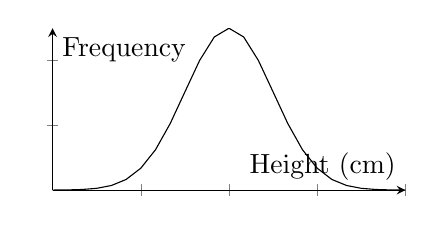
\begin{tikzpicture}
      \begin{axis}[
          width=0.5\textwidth,
          height=0.3\textwidth,
          xlabel={Height (cm)},
          ylabel={Frequency},
          xmin=150, xmax=190,
          ymin=0, ymax=0.05,
          yticklabels=\empty,
          xticklabels=\empty,
          axis lines=middle,
          scaled y ticks = false,
        ]
        \addplot[mark=none, domain=150:190] {0.05 * exp(-0.5 * ((x - 170) / 5) ^ 2)};
      \end{axis}
    \end{tikzpicture}
  \end{center}

  The normal distribution is the most common probability model in real life. A
  normal distribution consists of two parameters, the mean value $\mu$ and the
  standard deviation $\sigma$, thier corresponding functional expression of
  normal curve is:
  \begin{cequation}
    f(x) = \frac{1}{\sigma \sqrt{2\pi}} e^{-\frac{(x - \mu)^2}{2\sigma^2}}
  \end{cequation}

  Assume that the observation $X$ of a trial is normal distribution with mean
  value $\mu$ and standard deviation $\sigma$, then its denoted as:
  \begin{cequation}
    X \sim N(\mu, \sigma^2)
  \end{cequation}
  The probability $P$ ($a < X < b$) of the observation $X$ being in the interval $(a, b)$ is the area formed by the x-axis, line $x = a$, line $x = b$, and the normal curve, as shown in the figure below.

  \begin{center}

    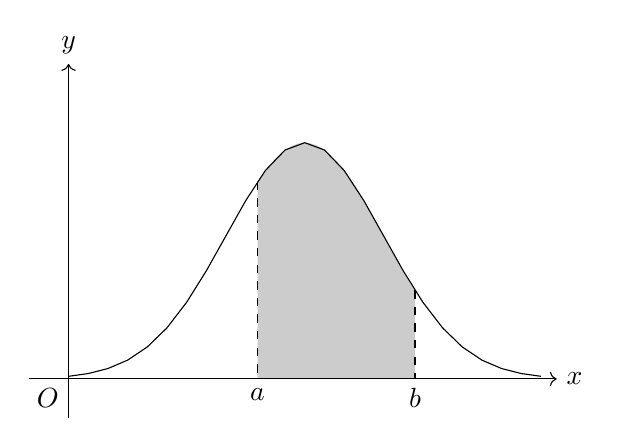
\begin{tikzpicture}
      % define normal distribution function 'normaltwo'
      \def\normaltwo{\x,{3*1/exp(((\x-3)^2)/2)}}

      % input x and y parameters
      \def\y{4.4}
      \def\x{2.4}

      % this line calculates f(y)
      \def\fy{3*1/exp(((\y-3)^2)/2)}
      \def\fx{3*1/exp(((\x-3)^2)/2)}

      % Shade orange area underneath curve.
      \fill [fill=gray!40] ({\x},0) -- plot[domain={\x}:{\y}] (\normaltwo) -- ({\y},0) -- cycle;

      % Draw and label normal distribution function
      \draw[domain=0:6] plot (\normaltwo) node[right] {};

      % Add dashed line dropping down from normal.
      \draw[dashed] ({\y},{\fy}) -- ({\y},0) node[below] {$b$};
      \draw[dashed] ({\x},{\fx}) -- ({\x},0) node[below] {$a$};

      % Optional: Add axis labels
      \draw (6.2, 0) node[right] {$x$};
      \draw (0, 4) node[above] {$y$};
      \draw (0, 0) node [below left] {$O$};

      % Optional: Add axes
      \draw[->] (-0.5,0) -- (6.2,0) node[above] {};
      \draw[->] (0,-0.5) -- (0,4) node[right] {};
    \end{tikzpicture}
  \end{center}

  A normal distribution with mean value of 0 and standard deviation of 1 is
  called the standard normal distribution, its normal curve
  \begin{cequation}
    f(x) = \frac{1}{\sqrt{2\pi}} e^{-\frac{x^2}{2}}
  \end{cequation}
  is symmetrical about y-axis, as shown in the figure below.

  \begin{center}
    \begin{tikzpicture}
      % define normal distribution function 'normaltwo'
      \def\normaltwo{\x,{3*1/exp(((\x)^2)/2)}}

      % Draw and label normal distribution function
      \draw[domain=-3:3] plot (\normaltwo) node[right] {};

      % Optional: Add axis labels
      \draw (3.2, 0) node[right] {$x$};
      \draw (0, 4) node[above] {$y$};
      \draw (0, 0) node [below left] {$O$};

      % Optional: Add axes
      \draw[->] (-3.2,0) -- (3.2,0) node[above] {};
      \draw[->] (0,-0.5) -- (0,4) node[right] {};

      \node at (2, 2.5) {$y=\frac{1}{\sqrt{2\pi}} e^{-\frac{x^2}{2}}$};
    \end{tikzpicture}
  \end{center}

  Assume that $X$ is a normal distribution with mean value $\mu$ and standard
  deviation $\sigma$, then
  \begin{cequation}
    Z = \frac{X - \mu}{\sigma}
  \end{cequation}
  is a standard normal distribution. That is,
  \begin{cequation}
    \text{If } x \sim N(\mu, \sigma^2), \text{ then } Z = \frac{x - \mu}{\sigma}\text{, } Z \sim N(0, 1)
  \end{cequation}

  Hence, General problems of normal distribution can be solved by converting into
  standard normal distribution problems.

  In order to calculate the probability of events related to standard normal
  distribution, we have attached a standard normal distribution table in appendix
  A. Assume that $Z$ is a standard normal distribution, $z$ is a positive number
  lesser than or equal to $3.49$, we can use the table to calculate the
  probability of $Q(z) = P(Z \leq z)$.

  For example, to find $P(Z \leq 1.23)$, first find the row of $z = 1.2$. The
  value in the column of this row corresponding to 3 (2nd decimal place) is
  $0.1093$, this is the probability of $P(Z \leq 1.23)$.
  \begin{center}
    \begin{tabular}{|c|c|c|c|c|c|}
      \hline
      $z$ & 0      & 1                     & 2      & 3               & $\cdots$ \\
      \hline
          &        & \multicolumn{3}{c|}{} &                                     \\
          &        & \multicolumn{3}{c|}{} &                                     \\
      \hline
      1.2 & 0.1151 & 0.1131                & 0.1112 & \textbf{0.1093} &          \\
      \hline
          &        & \multicolumn{3}{c|}{} &                                     \\
      \hline
    \end{tabular}
  \end{center}

  Any probability of events related to standard normal distribution can be solved
  using symmetry and properties of probability.

  Since the probability of sure event is 1, the area of the region under the
  curve of standard normal distribution above the x-axis is 1.

  Assume that $X$ is a normal distribution, $x$ is any real number, $P(X=x) = 0$.
  Therefore, $P(X < x) = P(X \leq x)$, $P(X > x) = P(X \geq x)$.

  \subsection{Practice 9}

  There are 2500 students who have attended geography exam during the Senior UEC
  exam. their marks can be assumed to be a normal distribution with mean value of
  60 and standard deviation of 11.
  \begin{enumerate}[label=(\alph*)]
    \item Find the number of students who failed the exam.
    \item If grade $A1$ is 78 marks or above, find the percentage of students who
          obtained grade $A1$.
    \item If the passing rate is $90\%$, find the minimum marks required to pass the
          exam. (Round to the nearest integer)
  \end{enumerate}

  \subsection{Exercise 21.6}

  \begin{enumerate}
    \item If the observation of a trial $Z$ is a standard normal distribution, find the
          probability of the following events:
          \begin{enumerate}
            \item $P(Z < 0.91)$
            \item $P(Z \leq -2.01)$
            \item $P(Z \geq -0.5)$
            \item $P(0.24 < Z \leq 1.79)$
            \item $P(-2.21 < Z < -0.97)$
            \item $P(-2.39 < Z \leq 0.56)$
          \end{enumerate}

    \item If the observation of a trial $Z$ is a standard normal distribution, find the
          value of $a$ of the following events:
          \begin{enumerate}
            \item $P(Z > a) = 0.0505$
            \item $P(Z < a) = 0.8980$
            \item $P(Z < a) = 0.3632$
            \item $P(Z > a) = 0.8599$
            \item $P(|Z| > a) = 0.0142$
            \item $P(|Z| < a) = 0.7888$
          \end{enumerate}

    \item A factory produces canned coffee. The capacity of each can can be assumed to be
          a normal distribution with mean value of $244.5ml$ and standard deviation of
          $5.4ml$.
          \begin{enumerate}
            \item Randomly pick a can of coffee, find the probability that the capacity of the
                  can is less than $235ml$.
            \item Randomly pick a can of coffee, find the probability that the capacity of the
                  can is in between $240ml$ and $250ml$.
            \item The factory has sold $18,000$ can of coffee in a week. How many cans have a
                  capacity greater than $260ml$?
            \item Someone has bought 7 cans of coffee, find the probability that 4 cans of coffee
                  have less than $2420ml$ of capacity each.
          \end{enumerate}

    \item A machine produces wrapped cookies, the weight of each cookie can be assumed to
          be a normal distribution with mean value of $501.25g$ and standard deviation of
          $5.32g$.
          \begin{enumerate}
            \item Find the percentage of cookies that have a weight less than $490g$.
            \item Of the $10,000$ cookies produced by the machine, how many cookies have a weight
                  greater than $510g$?
            \item If there are $2.5\%$ of the cookies that have a weight less than $a$ grams,
                  find the value of $a$.
            \item If there are $99.02\%$ of the cookies that have a weight between $(501.25 - c)$
                  grams and $(501.25 + c)$ grams, find the value of $c$.
          \end{enumerate}

    \item The life span of brand $A$ television can be assumed to be a normal
          distribution with mean value of $7.28$ years and standard deviation of $2.23$
          years. The warranty of the television is $3$ years. If the television is broken
          within the warranty period, the company will replace it with a new one for
          free. Find the percentage of television that will be replaced.

    \item The number of letters received by a company in a working day. Given that the
          probability of receiving more than 150 letters in a working day is $0.1210$,
          while the probability of receiving more than 50 letters in a working day is
          $0.9495$. Find the mean value and standard deviation of the number of letters
          received by the company in a working day.

    \item There are $2,256$ students sitting on the entrance exam for a high school. THe
          full marks of the exam is $400$ marks, and there are $1,200$ students who get
          accepted into the high school. The marks of the students can be assumed to be a
          normal distribution with mean value of $189$ marks and standard deviation of
          $53$.
          \begin{enumerate}
            \item Find the number of students who get less than $160$ marks.
            \item Find the lowest marks that a student can get to be accepted into the high
                  school. (Round to the nearest integer)
            \item If the students who get more than $300$ marks are eligible to get a
                  scholarship, find the number of students who are eligible to get a scholarship,
                  and their percentage.
            \item The school administration stipulates that the students who get less than $200$
                  marks has to take a remedial class. Find the number of students who have to
                  take a remedial class.
          \end{enumerate}

    \item A group of data is normally distributed with mean value of $\mu$ and standard
          deviation of $\sigma$. Find in this group of data:
          \begin{enumerate}
            \item The percentage of data that is in between $\mu - \sigma$ and $\mu + \sigma$.
            \item The percentage of data that is in between $\mu - 2\sigma$ and $\mu + 2\sigma$.
            \item The percentage of data that is in between $\mu - 3\sigma$ and $\mu + 3\sigma$.
          \end{enumerate}
  \end{enumerate}

  \section{Revision Exercise 21}

  \begin{enumerate}
    \item Tossing two dices at the same time, find the event where the sum of the two
          dices is $8$.

    \item There are 30 boys and 12 girls in a class. Randomly pick a representative, find
          the probability of a boy getting picked.

    \item Randomly pick a card from a deck of 52 poker card, find the probability of the
          following events:
          \begin{enumerate}
            \item Getting a spades.
            \item Not getting a spades.
          \end{enumerate}

    \item Randomly pick a card from a deck of 52 poker card, find the probability of the
          following events:
          \begin{enumerate}
            \item Getting a club.
            \item Getting an ace.
            \item Getting a club ace.
            \item Getting a club or an ace.
          \end{enumerate}

    \item Randomly write down a two digit number, find the probability of the following
          events:
          \begin{enumerate}
            \item Larger than 20.
            \item An even number.
            \item An odd number.
          \end{enumerate}

    \item Let a phone number consist of 7 digits formed by 0, 1, 2, $\cdots$, 9. Someone
          only remembers the first three digits and forgots the last four digits of the
          phone number of his colleague. Find the probability him calling the right
          person with just one dial.

    \item Person $A$ and $B$ toss two dices each at the same time. Person $B$ gets 10
          points, what is the probability of person $A$ winning?

    \item In a archery competition, the probability of person $A$ and person $B$ winning
          are $0.35$ and $0.45$ respectively. Find the probability of both of them
          losing.

    \item There are 200 staff members in a company, a quarter of which are foreigners.
          There are 115 male staff members and 85 female staff members in the company.
          Given that 20 female staff members are foreigners. Now randomly pick a staff
          member, find the probability of the staff member picked is male and a native.

    \item Drawing three cards from a deck of 52 poker card, find the probability of
          drawing at least one face card.

    \item The hit rate of a person shooting a basketball is $0.8$. If he shoots three
          times, find the probability of him scoring at least two times.

    \item The accuracy of forecast of a weather station is $89\%$. Find the probability
          of five accurate forecasts in a week.

    \item Given that the probability of a 18-year-old teenager being drawn for national
          service is $0.2$. Given that a community has 4 18-year-old teenagers, find the
          probability of at least one of them being drawn for national service.

    \item Tossing a dice, getting a number 6 can get $\$30$, while getting other numbers
          can get $\$3$. Find the expected value of the game.

    \item There are 4 50 cent coins and and 6 20 cent coins in a bag. A person randomly
          pick two coins from the bag. Find the expected value he gets.

    \item A food stall perpares 250 packets of nasi lemak every day. The cost of each
          packet is $\$1.50$, and the selling price is $\$5.00$, unsold packets are
          thrown away. According to statistical data, the stall can sell $57\%$ of the
          nasi lemaks. Find the expected value of the profit of the stall.

    \item In a lucky draw, there are 15 envelopes with cash prizes inside, one of which
          has $\$100$, two of which has $\$50$, three of which has $\$10$, four of which
          has $\$5$, and five of which has $\$1$. One person draw one envelope from the
          lucky draw, find the expected value. If the person pays $\$15$ to draw one
          envelope, determine whether it is worth it to pay for the lucky draw.

    \item The winning rate of a guessing game in a charity fair are as follows: winning
          the probabilities of $\$2,000$, $\$500$, $\$200$ are all $\frac{1}{5000}$,
          while the probability of winning $\$150$ is $\frac{1}{3000}$. If the fee to
          play the game once is $\$1$, find the expected value of the game. Is it worth
          it for the player to play the game?

    \item The weight distribution of $2,524$ girls in a school can be assumed to be a
          normal distribution with mean weight of $53.79kg$ and standard deviation of
          $7.24kg$.
          \begin{enumerate}
            \item Randomly pick a girl, find the probability of her weight being less than
                  $40kg$.
            \item Find the number of girls whose weight is greater than $65kg$.
            \item Find the percentage of girls whose weight is between $45kg$ and $55kg$.
            \item Assume that there are $10.03\%$ of the girls whose weight is greater than
                  $c$kg, find $c$.
            \item Randomly pick 10 girls, find the probability of at least two of them having
                  weight lesser than $55kg$.
          \end{enumerate}

    \item The duration of phone calls of customer service of a company can be assumed to
          be a normal distribution. Given that of all the phone calls, $1.02\%$ of them
          are more than $30$ minutes long, $25.14\%$ of them are less than $20$ minutes
          long. Find the mean value and standard deviation of the duration of phone
          calls.
  \end{enumerate}

\end{multicols}

\appendix

\chapter{Standard Normal Distribution Table}

Listed in the table below are $Q(z) = P(Z \leq z)$, in which $Z$ is a standard
normal distribution $N(0, 1)$.

\begin{center}
  \begin{tabular*}{\linewidth}{@{\extracolsep{\fill}} |c|c|ccc|ccc|ccc|}
    \hline
    $z$ & 0      & 1      & 2      & 3      & 4      & 5      & 6      & 7      & 8      & 9      \\
    \hline
    \\[-1em]
    0.0 & 0.5000 & 0.4960 & 0.4920 & 0.4880 & 0.4840 & 0.4801 & 0.4761 & 0.4721 & 0.4681 & 0.4641 \\
    \\[-1em]
    0.1 & 0.4602 & 0.4562 & 0.4522 & 0.4483 & 0.4443 & 0.4404 & 0.4364 & 0.4325 & 0.4286 & 0.4247 \\
    \\[-1em]
    0.2 & 0.4207 & 0.4168 & 0.4129 & 0.4090 & 0.4052 & 0.4013 & 0.3974 & 0.3936 & 0.3897 & 0.3859 \\
    \\[-1em]
    0.3 & 0.3821 & 0.3783 & 0.3745 & 0.3707 & 0.3669 & 0.3632 & 0.3594 & 0.3557 & 0.3520 & 0.3483 \\
    \\[-1em]
    0.4 & 0.3446 & 0.3409 & 0.3372 & 0.3336 & 0.3300 & 0.3264 & 0.3228 & 0.3192 & 0.3156 & 0.3121 \\
    \\[-1em]
    \hline
    \\[-1em]
    0.5 & 0.3085 & 0.3050 & 0.3015 & 0.2981 & 0.2946 & 0.2912 & 0.2877 & 0.2843 & 0.2810 & 0.2776 \\
    \\[-1em]
    0.6 & 0.2743 & 0.2709 & 0.2676 & 0.2643 & 0.2611 & 0.2578 & 0.2546 & 0.2514 & 0.2483 & 0.2451 \\
    \\[-1em]
    0.7 & 0.2420 & 0.2389 & 0.2358 & 0.2327 & 0.2296 & 0.2266 & 0.2236 & 0.2206 & 0.2177 & 0.2148 \\
    \\[-1em]
    0.8 & 0.2119 & 0.2090 & 0.2061 & 0.2033 & 0.2005 & 0.1977 & 0.1949 & 0.1922 & 0.1894 & 0.1867 \\
    \\[-1em]
    0.9 & 0.1841 & 0.1814 & 0.1788 & 0.1762 & 0.1736 & 0.1711 & 0.1685 & 0.1660 & 0.1635 & 0.1611 \\
    \\[-1em]
    \hline
    \\[-1em]
    1.0 & 0.1587 & 0.1562 & 0.1539 & 0.1515 & 0.1492 & 0.1469 & 0.1446 & 0.1423 & 0.1401 & 0.1379 \\
    \\[-1em]
    1.1 & 0.1357 & 0.1335 & 0.1314 & 0.1292 & 0.1271 & 0.1251 & 0.1230 & 0.1210 & 0.1190 & 0.1170 \\
    \\[-1em]
    1.2 & 0.1151 & 0.1131 & 0.1112 & 0.1093 & 0.1075 & 0.1056 & 0.1038 & 0.1020 & 0.1003 & 0.0985 \\
    \\[-1em]
    1.3 & 0.0968 & 0.0951 & 0.0934 & 0.0918 & 0.0901 & 0.0885 & 0.0869 & 0.0853 & 0.0838 & 0.0823 \\
    \\[-1em]
    1.4 & 0.0808 & 0.0793 & 0.0778 & 0.0764 & 0.0749 & 0.0735 & 0.0721 & 0.0708 & 0.0694 & 0.0681 \\
    \\[-1em]
    \hline
    \\[-1em]
    1.5 & 0.0668 & 0.0655 & 0.0643 & 0.0630 & 0.0618 & 0.0606 & 0.0594 & 0.0582 & 0.0571 & 0.0559 \\
    \\[-1em]
    1.6 & 0.0548 & 0.0537 & 0.0526 & 0.0516 & 0.0505 & 0.0495 & 0.0485 & 0.0475 & 0.0465 & 0.0455 \\
    \\[-1em]
    1.7 & 0.0446 & 0.0436 & 0.0427 & 0.0418 & 0.0409 & 0.0401 & 0.0392 & 0.0384 & 0.0375 & 0.0367 \\
    \\[-1em]
    1.8 & 0.0359 & 0.0351 & 0.0344 & 0.0336 & 0.0329 & 0.0322 & 0.0314 & 0.0307 & 0.0301 & 0.0294 \\
    \\[-1em]
    1.9 & 0.0287 & 0.0281 & 0.0274 & 0.0268 & 0.0262 & 0.0256 & 0.0250 & 0.0244 & 0.0239 & 0.0233 \\
    \\[-1em]
    \hline
    \\[-1em]
    2.0 & 0.0228 & 0.0222 & 0.0217 & 0.0212 & 0.0207 & 0.0202 & 0.0197 & 0.0192 & 0.0188 & 0.0183 \\
    \\[-1em]
    2.1 & 0.0179 & 0.0174 & 0.0170 & 0.0166 & 0.0162 & 0.0158 & 0.0154 & 0.0150 & 0.0146 & 0.0143 \\
    \\[-1em]
    2.2 & 0.0139 & 0.0136 & 0.0132 & 0.0129 & 0.0125 & 0.0122 & 0.0119 & 0.0116 & 0.0113 & 0.0110 \\
    \\[-1em]
    2.3 & 0.0107 & 0.0104 & 0.0102 & 0.0099 & 0.0096 & 0.0094 & 0.0091 & 0.0089 & 0.0087 & 0.0084 \\
    \\[-1em]
    2.4 & 0.0082 & 0.0080 & 0.0078 & 0.0075 & 0.0073 & 0.0071 & 0.0069 & 0.0068 & 0.0066 & 0.0064 \\
    \\[-1em]
    \hline
    \\[-1em]
    2.5 & 0.0062 & 0.0060 & 0.0059 & 0.0057 & 0.0055 & 0.0054 & 0.0052 & 0.0051 & 0.0049 & 0.0048 \\
    \\[-1em]
    2.6 & 0.0047 & 0.0045 & 0.0044 & 0.0043 & 0.0041 & 0.0040 & 0.0039 & 0.0038 & 0.0037 & 0.0036 \\
    \\[-1em]
    2.7 & 0.0035 & 0.0034 & 0.0033 & 0.0032 & 0.0031 & 0.0030 & 0.0029 & 0.0028 & 0.0027 & 0.0026 \\
    \\[-1em]
    2.8 & 0.0026 & 0.0025 & 0.0024 & 0.0023 & 0.0023 & 0.0022 & 0.0021 & 0.0021 & 0.0020 & 0.0019 \\
    \\[-1em]
    2.9 & 0.0019 & 0.0018 & 0.0018 & 0.0017 & 0.0016 & 0.0016 & 0.0015 & 0.0015 & 0.0014 & 0.0014 \\
    \\[-1em]
    \hline
    \\[-1em]
    3.0 & 0.0013 & 0.0013 & 0.0013 & 0.0012 & 0.0012 & 0.0011 & 0.0011 & 0.0011 & 0.0010 & 0.0010 \\
    \\[-1em]
    3.1 & 0.0010 & 0.0009 & 0.0009 & 0.0009 & 0.0009 & 0.0008 & 0.0008 & 0.0008 & 0.0007 & 0.0007 \\
    \\[-1em]
    3.2 & 0.0007 & 0.0007 & 0.0006 & 0.0006 & 0.0006 & 0.0006 & 0.0006 & 0.0005 & 0.0005 & 0.0005 \\
    \\[-1em]
    3.3 & 0.0005 & 0.0005 & 0.0005 & 0.0004 & 0.0004 & 0.0004 & 0.0004 & 0.0004 & 0.0004 & 0.0003 \\
    \\[-1em]
    3.4 & 0.0003 & 0.0003 & 0.0003 & 0.0003 & 0.0003 & 0.0003 & 0.0003 & 0.0003 & 0.0003 & 0.0002 \\
    \hline
  \end{tabular*}
\end{center}

\end{document}